\documentclass[12pt,a4paper,openright,twoside]{book}

\usepackage{tese_new}
\usepackage[portuguese]{babel}   %Português 
\usepackage{rotating,hyperref,amsfonts,graphicx,amssymb,algorithmic,booktabs}
\usepackage{algorithm}
\usepackage{amsmath}
\usepackage{xspace}
\usepackage{color}
\usepackage{fancyhdr}
\usepackage[style=apa, backend=biber]{biblatex}
\addbibresource{references.bib} % Nome do teu ficheiro .bib

%\usepackage[math]{iwona}
\usepackage[printonlyused]{acronym}
\usepackage{float}
\usepackage{amssymb}
\usepackage{amsfonts}
\usepackage{latexsym}
\usepackage{tocbibind}
\usepackage{wrapfig}
\usepackage[small,normal,bf,up]{caption}
\usepackage{verbatim}
\usepackage{semantic}
\usepackage{listings}
\usepackage[final]{pdfpages}
\usepackage{appendix}
\usepackage{multicol}
\usepackage{media9}
\usepackage{multirow}
\usepackage{url}
\usepackage{todonotes}
\usepackage{fontspec}
\setmainfont{Georgia}
\setsansfont{Georgia}
\setmonofont{Georgia}
%
\usepackage{subcaption}
%

\def\tablesthickness{0.05cm}
\def\arraystretchtables{0.85}
\def\tabcolseptables{6pt}
\def\tamanhoROC{200pt}
\def\tamanhoHistograma{200pt}
\def\tamanhoFiguraBi{150pt}
\def\tamanhoFiguraTri{250pt}
\def\tamanhoIrisNormalizada{250pt}


\renewcommand{\labelitemi}{-}
\renewcommand{\labelitemii}{\bullet}
\renewcommand{\labelitemiii}{\circ}

\makeindex
\raggedbottom
\begin{document}
%\fontfamily{tpm}\selectfont
\frontmatter
\pagestyle{empty}

%\thispagestyle{empty}

\topmargin -0.3in

\begin{flushright}

\includegraphics[width=3.0cm]{images/logo_ubi_vprincipal.jpg}

\vspace{5.5cm}

\bf{\huge{PORT 0}}\\

\vspace{1.5cm}

\bf{\large{José Miguel Alves Melo dos Santos}}


\vspace{1.0cm}

Dissertação para obtenção do Grau de Mestre em\\
\textbf{\large{Design e Desenvolvimento de Jogos Digitais}}\\
(2º ciclo de estudos)

\vspace*{3.0cm}

\large{ 
Orientador: Doutor Frutuoso Gomes Mendes da Silva }

\vspace*{1.0cm}

\large{{Covilhã,  Junho 2026}}

\end{flushright}

\clearpage{\pagestyle{empty}\cleardoublepage}
%\thispagestyle{empty}



\clearpage{\pagestyle{empty}\cleardoublepage}

%\addtocounter{secnumdepth}{-1}
%\setcounter{secnumdepth}{-1}
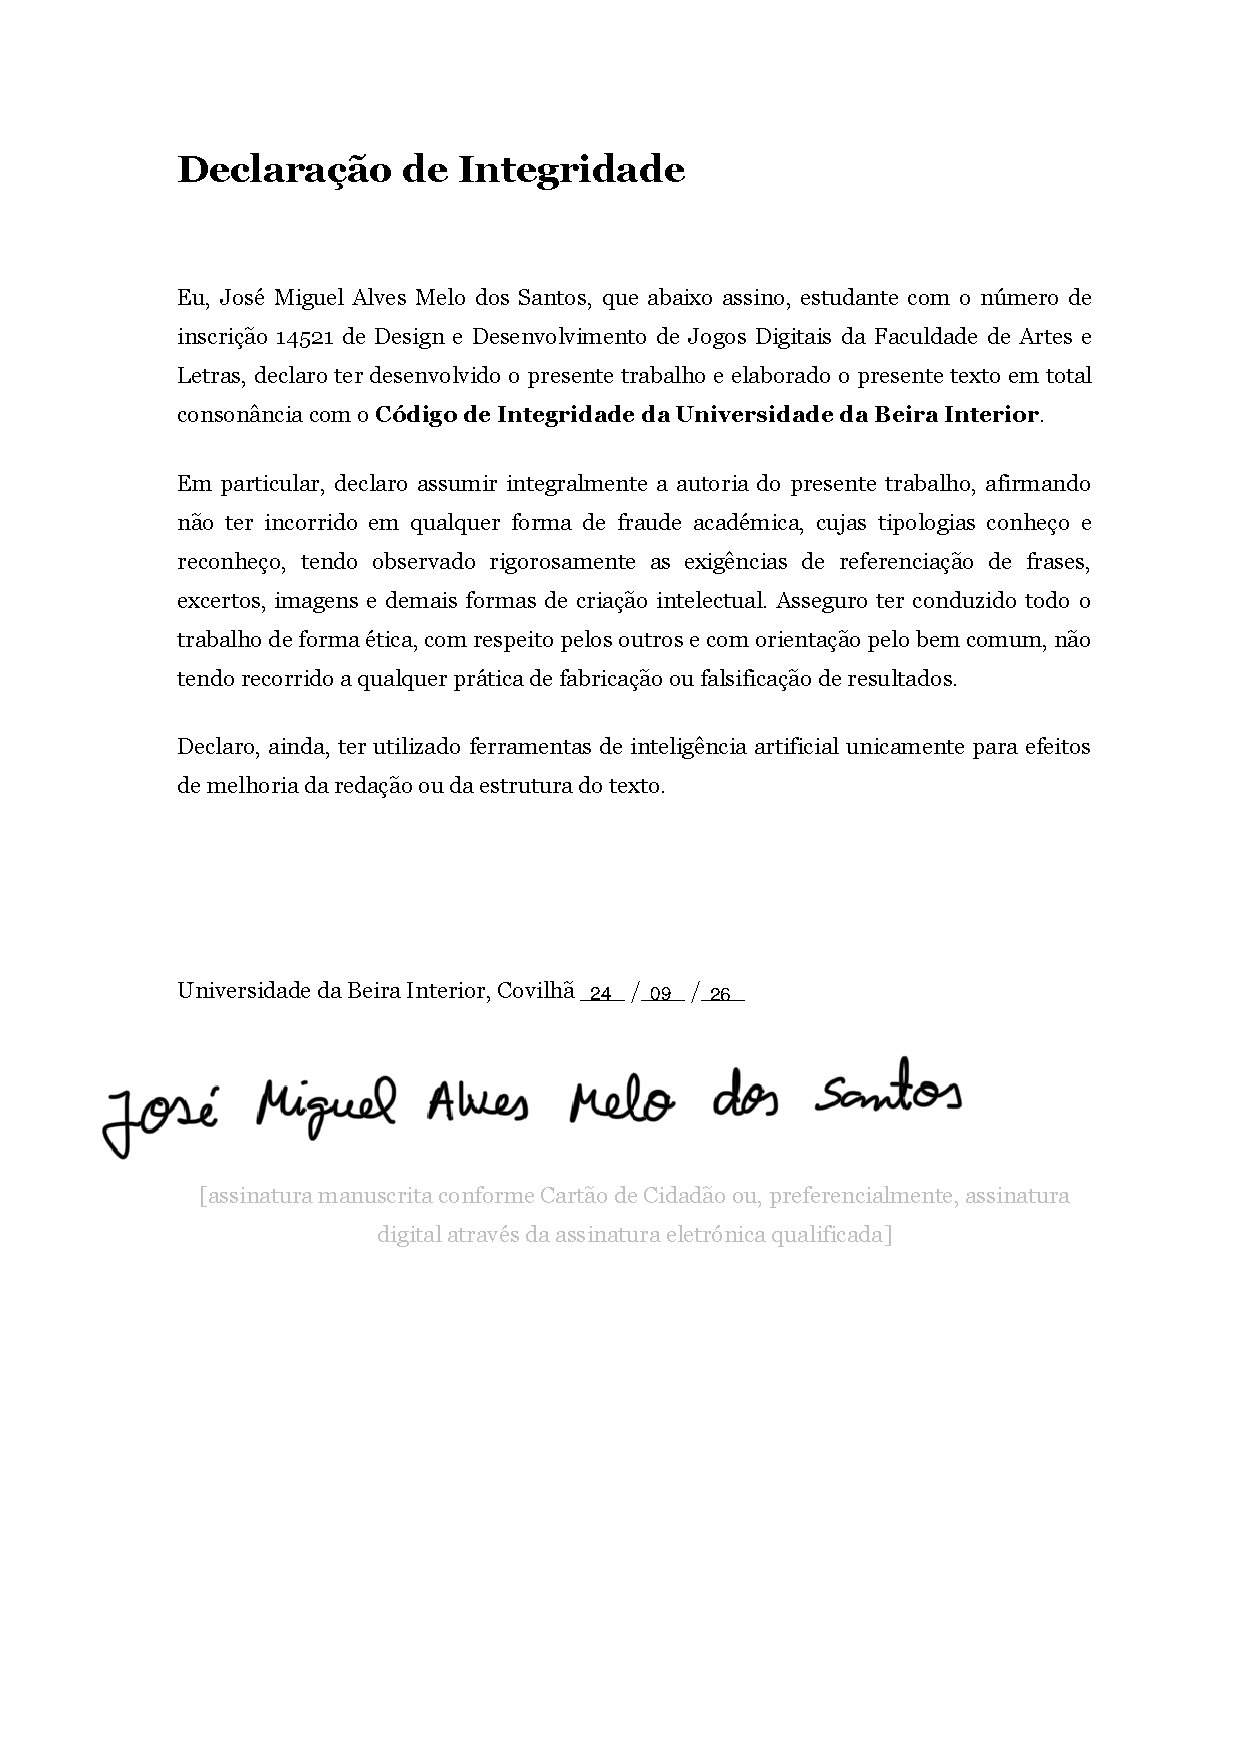
\includepdf[pages=-]{PDF/Declaracao-Integridade.pdf}

\includepdf[pages=-]{PDF/Copyright-Notice-PT-585.pdf}

\clearpage{\pagestyle{empty}\cleardoublepage}

%\addtocounter{secnumdepth}{-1}
%\setcounter{secnumdepth}{-1}
%\chapter{Agradecimentos}
\chapter{Agradecimentos}
\label{chap:agr}

Para começar, agradeço ...

Agradeço a todos pela ajuda ao longo desta jornada. 

Que o futuro reserve mais.



Trabalho desenvolvido no "Instituto de Telecomunicações"  sob orientação do Prof. Frutuoso Silva. 




%\addtocounter{secnumdepth}{-1}
%\setcounter{secnumdepth}{-1}
\chapter{Resumo}
\label{chap:resumo}

O presente trabalho apresenta o desenvolvimento de um videojogo inovador de simulação e gestão estratégica de infraestruturas tecnológicas, que combina a complexidade e o rigor técnico do ecossistema de computação com uma experiência lúdica altamente envolvente. Ao assumir o papel de gestor de um \textit{data center}, o jogador é desafiado a garantir a viabilidade económica da sua operação através da otimização de recursos financeiros, alocação de energia e seleção de componentes de \textit{hardware} reais.


Desenvolvido no motor Unity e aliado a metodologias sólidas de game design, como os \textit{frameworks} \ac{MDA}, \textit{Flow} e o Modelo de Hook, o produto destaca-se por transformar o conhecimento técnico em ferramentas essenciais de progressão. A inclusão de mecânicas dinâmicas de combate contra ameaças cibernéticas e de \textit{minigames} baseados em terminais virtuais (\textit{WordRush}) permite quebrar a monotonia da simulação económica, garantindo um ritmo contínuo de adrenalina e retenção do jogador.

Testado e avaliado com utilizadores reais, o videojogo demonstrou um elevado potencial na transmissão indireta de conceitos avançados de \ac{TI} e cibersegurança, traduzindo-se numa solução de entretenimento educativo pronta a capturar o interesse de entusiastas de jogos de estratégia, simulação e tecnologia.

\section*{Palavras-chave}
Jogo Educacional, Jogos Sérios, Jogo de Matemática, Unity

%\addtocounter{secnumdepth}{-1}
%\setcounter{secnumdepth}{-1}
\chapter{Abstract}
\label{chap:abstract}

This work ....

\section*{Keywords:}
Educational Games, Serious Games, Math Games, Unity

\clearpage{\pagestyle{empty}\cleardoublepage}

\afterpreface

\clearpage{\pagestyle{empty}\cleardoublepage}

\listoftables

%\clearpage{\pagestyle{empty}\cleardoublepage}

\chapter*{Acrónimos}
\label{chap:acro}

% #   ATENÇÃO
% A lista de acrónimods deve ser ordenada alfanumericamente.
% Estrangeirismos devem ser realçados em itálico.
% Se o relatório for escrito em Inglês, uma palavra portuguesa é um estrangeirismo.

% O maior acrónimo deve ser colocado neste ponto (reparar que CFIUTE é maior que TCP!).
%               vvvvvv
\begin{acronym}[MDA]
    \acro{MDA}{Mechanics, Dynamics and Aesthetics}
    \acro{UBI}{Universidade da Beira Interior}
    \acro{RPG}{Role-Playing Game}
    \acro{UI}{User Interface}
    \acro{UX}{User Experience}
    \acro{CLI}{\textit{Command Line Interface}}
    \acro{IA}{Inteligência Artificial}
    \acro{VFX}{\textit{Visual Effects}}
\end{acronym}

\clearpage{\pagestyle{empty}\cleardoublepage}

\mainmatter

%Include here your chapters
%\setcounter{secnumdepth}{+2}
\chapter{Introdução}
%\chapter{Introduction}
\label{cap1}

\section{Introdução}

O presente trabalho surge no âmbito do Mestrado em Design e Desenvolvimento de 
Jogos Digitais da \ac{UBI} e foca-se na conceção e implementação de um videojogo de 
simulação e gestão de infraestruturas tecnológicas. O projeto propõe uma 
experiência imersiva onde o jogador assume o papel de gestor de um pequeno 
centro de dados (data center), tendo como objetivo primordial a viabilidade 
económica da operação por uma gestão estratégica de recursos. A abordagem 
adotada procura equilibrar o rigor técnico de conceitos reais de computação com 
o entretenimento, utilizando métricas e componentes de hardware autênticos para 
reforçar a imersão do utilizador.

A estrutura deste relatório de projeto reflete o percurso de desenvolvimento do jogo, 
começando por contextualizar a relevância do tema e as motivações que levaram à 
sua escolha. Ao longo dos capítulos subsequentes, é apresentado o estado da arte, 
onde se analisam títulos de referência no mercado e literatura científica relevante, 
seguido do detalhe das decisões de design e das técnicas de implementação utilizadas. 
Finalmente, o documento descreve os processos de teste e avaliação que validam o protótipo 
desenvolvido, culminando numa reflexão sobre as contribuições do trabalho e as perspetivas 
para desenvolvimentos futuros na área dos jogos educativos e de simulação.

\section{Motivação}

A motivação para o desenvolvimento deste projeto surge da intersecção entre 
a complexidade da gestão de infraestruturas tecnológicas e o potencial lúdico 
dos simuladores modernos. Embora o tema de gestão de data centers possa parecer,
à primeira vista, estritamente técnico ou árido, existe um ecossistema rico 
em mecânicas de estratégia, logística e resolução de problemas que se 
traduzem naturalmente em experiências de jogo envolventes.

Um dos principais motores deste trabalho é a vontade de desmistificar 
conceitos de computação de alto desempenho, como o consumo energético em Watts 
ou a capacidade de processamento em TFLOPS, integrando-os num ciclo de jogo 
onde o conhecimento é uma ferramenta para o sucesso e não uma barreira à 
entrada. A utilização de unidades e métricas reais visa reforçar a imersão e 
conferir um peso estratégico às decisões do jogador, permitindo uma aprendizagem 
orgânica através da simulação.

Contudo, a motivação central não reside apenas na simulação fiel, mas sim na 
criação de um produto onde a diversão é o fator predominante. Ao contrário de 
simuladores puramente técnicos, este projeto adota uma estética inspirada na 
ficção e elementos de fantasia para garantir um ambiente visualmente apelativo 
e menos formal. A inclusão de sistemas de combate e mini-jogos baseados em 
terminais virtuais serve o propósito vital de quebrar a monotonia da gestão 
económica, introduzindo dinamismo e momentos de adrenalina que mantêm o jogador 
num estado de flow constante.

Em suma, este projeto é motivado pela convicção de que é possível construir um 
jogo "sério" que não se leve demasiado a sério. O objetivo é proporcionar uma 
experiência recompensadora onde o jogador se sinta instigado a otimizar o seu 
centro de dados, não por obrigação académica, mas pelo puro entretenimento de 
superar desafios, gerir recursos e proteger a sua infraestrutura num universo 
digital vibrante.

\subsection{Organização do Documento}

O presente documento encontra-se estruturado em seis capítulos, os quais refletem as diferentes etapas do ciclo de desenvolvimento do projeto, desde a sua concetualização e fundamentação teórica até à implementação, testagem e reflexão crítica dos resultados obtidos. A organização dos capítulos apresenta-se da seguinte forma:

\begin{enumerate}
    \item \textbf{Introdução}: Este capítulo contextualiza o enquadramento geral do trabalho, apresentando a temática da simulação e gestão de \textit{data centers}. São detalhadas as motivações subjacentes ao projeto, os objetivos a atingir, a metodologia adotada e a estrutura formal deste relatório, acompanhada pela respetiva calendarização das tarefas.

    \item \textbf{Estado da Arte}: Apresenta uma análise crítica do panorama atual, dividida entre o estudo de videojogos comerciais de referência na área da simulação, montagem e gestão tecnológica (\textit{e.g.}, \textit{Data Center Demo}, \textit{PC Building Simulator}, \textit{Startup Company}, \textit{Grey Hack} e \textit{Software Inc.}) e a revisão de literatura científica relevante sobre jogos sérios, aprendizagem indireta e mecânicas de jogo.

    \item \textbf{Técnicas e Decisões de Design}: Descreve a fundamentação teórica do \textit{game design}, abordando os modelos e \textit{frameworks} aplicados (\textit{MDA}, \textit{Flow} e Modelo de \textit{Hook}). Adicionalmente, detalha as decisões criativas e concetuais relativas à interface de utilizador (\textit{UI/UX}), \textit{level design}, sistemas de notificação e correio eletrónico, referências estéticas para os elementos 3D, bem como as mecânicas de economia, configuração de equipamento e combate.

    \item \textbf{Implementação do Jogo}: Expõe o processo prático de desenvolvimento do videojogo, discriminando as ferramentas e tecnologias utilizadas (como o motor \textit{Unity}, o \textit{software Blender}, linguagens de programação e ferramentas de apoio com Inteligência Artificial). Inclui a engenharia de software (diagramas de arquitetura de sistema e casos de uso), a criação de modelos 3D e \textit{assets} 2D, e o desenvolvimento técnico de subsistemas fulcrais, tais como o sistema de ataques/defesa e o \textit{minigame} \textit{WordRush}.

    \item \textbf{Testes e Avaliação do Jogo}: Detalha a metodologia de teste aplicada com utilizadores reais e a consequente recolha de dados quantitativos e qualitativos. Este capítulo abrange a análise da \ac{UX} com base nas heurísticas de usabilidade de Nielsen, a avaliação do conhecimento técnico transmitido aos jogadores (através de questionários pré e pós-jogo) e o estudo dos dados analíticos/telemetria recolhidos durante as sessões de jogo.

    \item \textbf{Conclusões e Trabalho Futuro}: Sintetiza as principais conclusões retiradas ao longo do projeto, destacando o cumprimento dos objetivos propostos e as contribuições concretas do trabalho. Por fim, são perspetivadas várias linhas de desenvolvimento futuro e melhorias a implementar em edições subsequentes do jogo.
\end{enumerate}

\section{Calendarização do projeto}
\todo{Revisar}

A Tabela \ref{tab:Calendario}, apresenta a calendarização do projeto. É de notar que as tarefas apresentadas foram realizadas de forma intercalada.

\begin{table}[H]
\begin{tabular}{|l|r|}
\textbf{Tarefa} & \textbf{Duração} \\ \hline
Prototipagem rápida e busca de referências & 1 mês \\ \hline
Implementação do \textit{minigame WordRush} & 1 mês \\ \hline
Design dos sistemas & 1 mês \\ \hline
Implementação dos sistemas & 2,5 meses \\ \hline
Referências visuais de 3D e \ac{VFX} & 1 mês \\ \hline
Criação dos \ac{VFX} e dos modelos 3D & 1 mês \\ \hline
Implementação de efeitos sonos e narração & 1 semana \\ \hline
Correção de \textit{bugs} & 1 mês \\ \hline
Realização dos testes & 1 mês \\ \hline
Escrita do relatório & 2 meses \\ \hline
\end{tabular}
\centering
\caption{Calendarização do projeto}
\label{tab:Calendario}
\end{table}

\todo{Aqui}

\chapter{Estado da Arte}

\section{Introdução}

O presente capítulo tem como finalidade apresentar o estado da arte relativo à temática em análise, reunindo e examinando criticamente as principais contribuições científicas e jogos desenvolvidas até ao momento. A compreensão do panorama atual do conhecimento revela-se fundamental para enquadrar o projeto.

Neste capítulo serão, assim, analisados um conjunto de jogos e artigos, procurando estabelecer um enquadramento crítico que permita compreender a evolução do conhecimento na área e sustentar o desenvolvimento apresentado nos capítulos subsequentes.

\section{Vídeo Jogos}

\subsection{Data Center Demo}

\begin{figure}[H]
\centering
\begin{tabular}{ll}

\begin{minipage}{0.55\textwidth}
\textcite{DataCenterDemo} está a desenvolver o jogo
    Data Center (ver Figura \ref{DataCenter_Capa}), que atualmente está em versão Demo na Steam
    e com previsão de lançamento para
    o dia 31 de março de 2026, é um jogo do estilo simulador técnico que foca na representação tridimensional e na gestão de infraestruturas de TI. Ao contrário de jogos puramente recreativos, a sua prioridade é a fidelidade técnica e a visualização de métricas em tempo real.
    Alguns dos pontos mais explorados por ele são:
\end{minipage}
&
\begin{minipage}{0.35\textwidth}
\centering

\includegraphics[width=\textwidth]{images/DataCenterCapa.jpg}
\caption[Data Center Demo - Capa do jogo. Retirado de \url{https://store.steampowered.com/app/4376050/Data_Center_Demo}]{Data Center Demo - Capa do jogo.}
\label{DataCenter_Capa}
\end{minipage}
\end{tabular}
\end{figure}


\begin{itemize}
  \item Gestão de Infraestrutura Física:
  Apresenta para o jogador a disposição das \textit{racks}, unidades de distribuição de energia (PDUs) e sistemas de arrefecimento (CRACs). Demonstrando como o layout físico impacta diretamente a eficiência operacional (ver Figura \ref{DataCenter_Gameplay1}).
O jogador terá de fazer a instalação de uma infraestrutura passando pela várias etapas, como montagem, conexão de cabos e configuração de equipamentos.
  \begin{figure}[h]
    \centering
    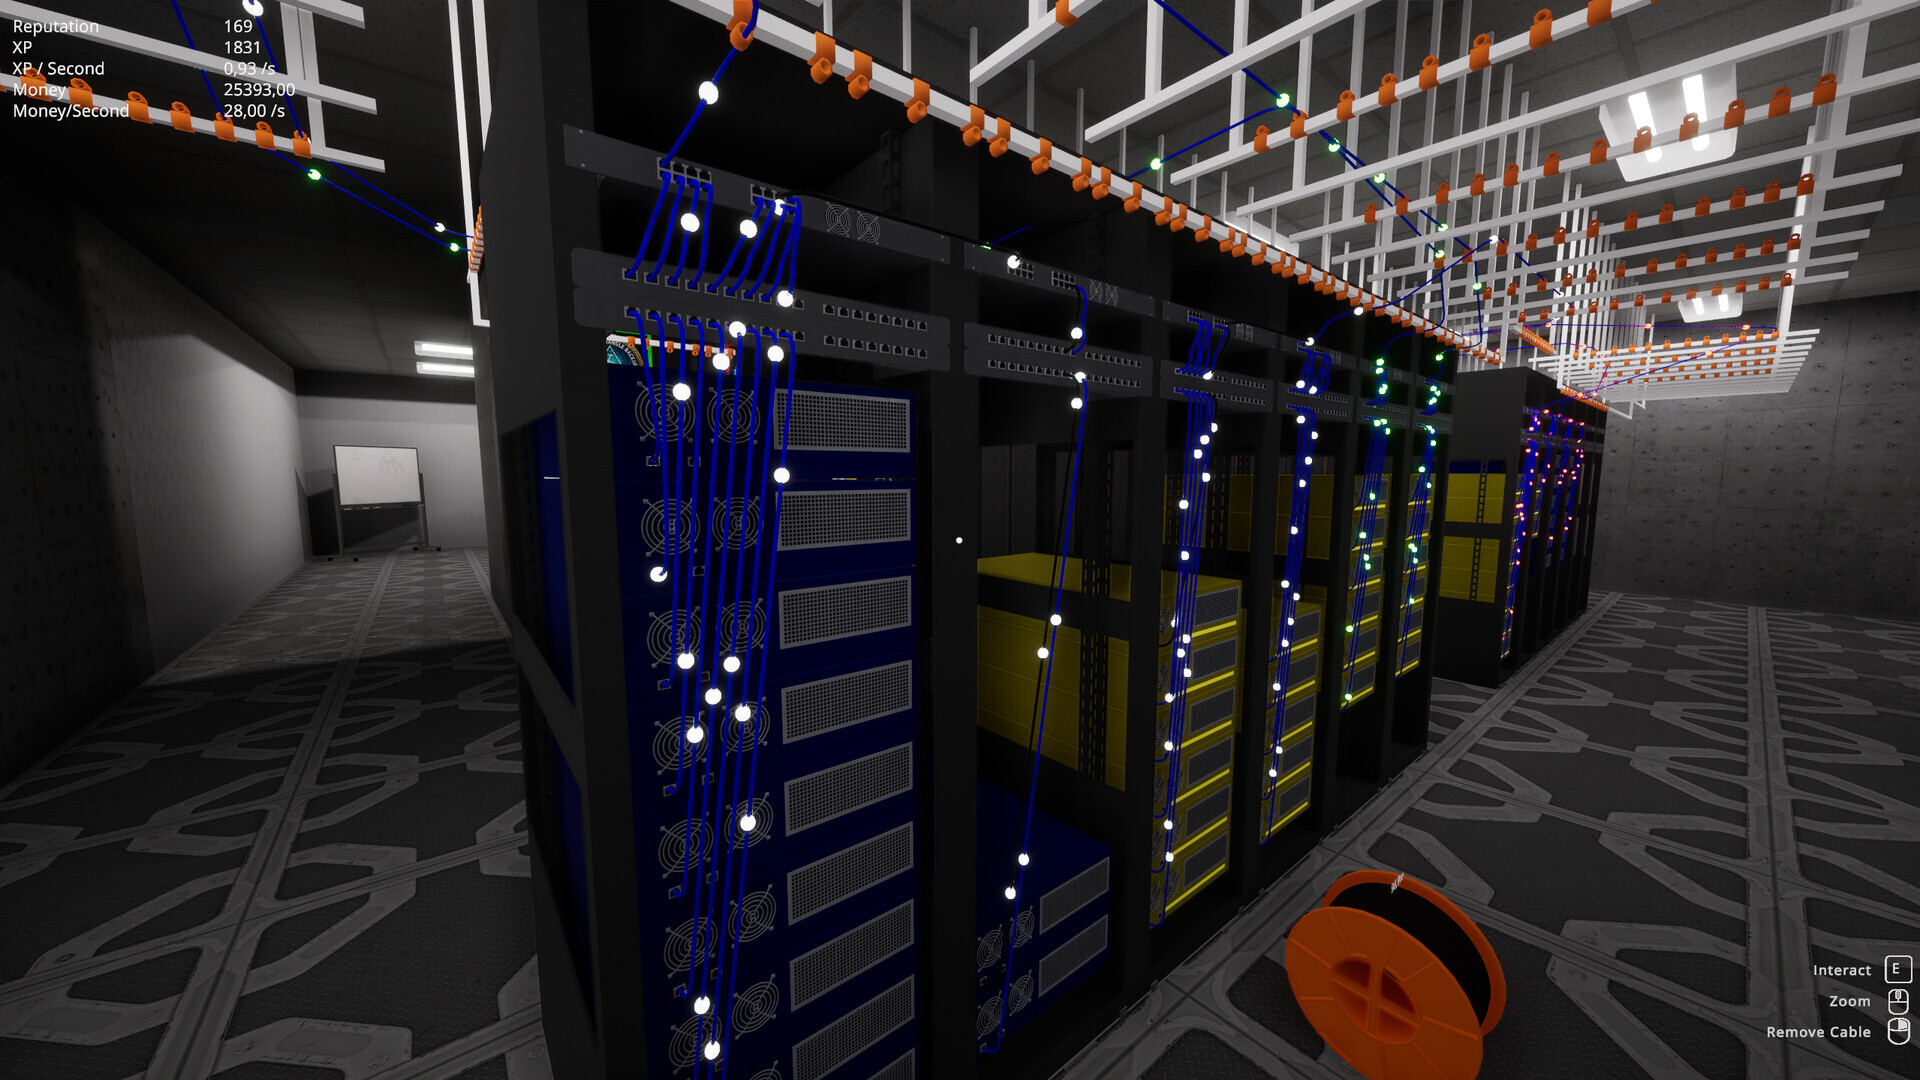
\includegraphics[width=0.8\textwidth]{images/DataCenter1.jpg}
    \caption[Data Center Demo - Configuração de \textit{racks}, ligação de cabos. Retirado de \url{https://store.steampowered.com/app/4376050/Data_Center_Demo}]{Data Center Demo - Configuração de racks, ligação de cabos.}
    \label{DataCenter_Gameplay1}
  \end{figure}
  \item Visualização Térmica:
  Uma das funcionalidades mais marcantes é a simulação de fluxo de ar e calor. O "jogo" mostra visualmente o impacto de corredores quentes e frios, permitindo que o jogador identifique \textit{hotspots} que poderiam levar à falha do \textit{hardware}.
  \item Simulação de Carga e Falhas:
  Permite ao jogador simular picos de tráfego ou falhas em componentes específicos (como a queda de um gerador ou UPS) para observar como o sistema de redundância reage.
  \item Métricas de Sustentabilidade:
  O \textit{software} calcula e apresenta indicadores de desempenho como o PUE (Power Usage Effectiveness).
\end{itemize}

\vspace{0.5cm}

O projeto desenvolvido apresenta diversas semelhanças com o Data Center Demo, nomeadamente ao nível do contexto de jogo, da tipologia de objetos representados e do cenário. Contudo, essas características são retratadas de forma mais simplificada e incluem alguns elementos de fantasia. A principal intenção é privilegiar a componente lúdica e a experiência de entretenimento, sem, no entanto, excluir por completo os elementos técnicos subjacentes à simulação.

\subsection{PC Building Simulator}

\begin{figure}[H]
\centering
\begin{tabular}{ll}

\begin{minipage}{0.55\textwidth}
\textcite{PCBuildingSimulator} desenvolveu o PC Building Simulator (ver Figura \ref{PCBuild_Capa}) com a proposta de ser um jogo de montagem de computadores, que permite ao jogador passar pelas várias etapas de montagem de um computador pessoal. O jogo destaca-se pela representação fiel de componentes e pela introdução de conceitos técnicos como compatibilidade de \textit{sockets}.
\end{minipage}
&
\begin{minipage}{0.35\textwidth}
\centering

\includegraphics[width=\textwidth]{images/PCBuildSimulator-Header.jpg}
\caption[PC Building Simulator - Capa do jogo. Retirado de \url{https://store.steampowered.com/app/621060/PC_Building_Simulator}]{PC Building Simulator - Capa do jogo. }
\label{PCBuild_Capa}
\end{minipage}
\end{tabular}
\end{figure}

\begin{itemize}
    \item Instalação de \textit{hardware}, desde da colocação de \textit{hardware} até conexão de cabos;
    \item Instalação de sistemas operativos;
    \item Instalação de \textit{softwares} adicionais e realização de teste.
\end{itemize}

O jogo destaca-se pela representação fiel de componentes (CPU,GPU,RAM,etc...) e pela
introdução de conceitos técnicos como compatibilidade de \textit{sockets} (ver Figura \ref{PCBuild_Gameplay1}).

\begin{figure}[H]
  \centering
  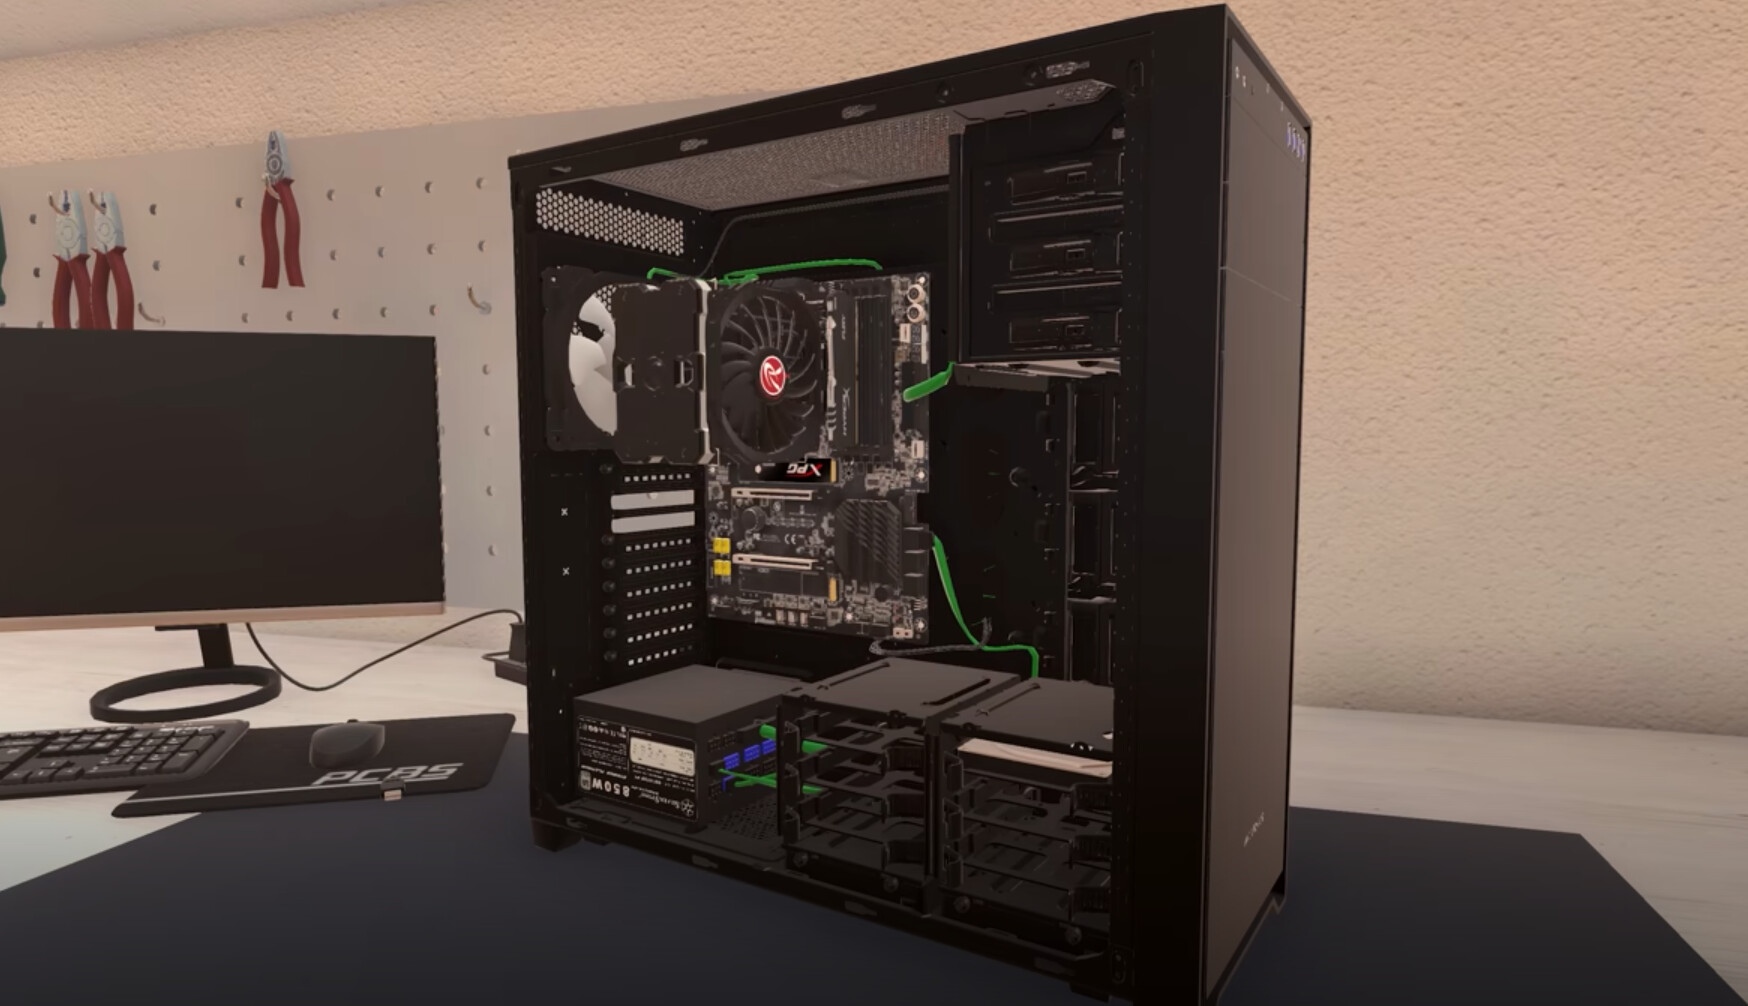
\includegraphics[width=0.8\textwidth]{images/PCBuildSimulator_BuildPC.jpg}
  \caption[PC Building Simulator - Montagem de um computador. Retirado de \url{https://store.steampowered.com/app/621060/PC_Building_Simulator}]{PC Building Simulator - Montagem de um computador.}
  \label{PCBuild_Gameplay1}
\end{figure}

A representação realista do hardware, bem como a simulação da instalação de sistemas operativos, foram também retratadas no projecto desenvolvido, ainda que de forma mais simplificada, lúdica e adaptada ao respectivo contexto.
Importa salientar que, à data da redação deste texto, já se encontra disponível o PC Building Simulator 2. No entanto, para efeitos deste trabalho, os aspetos apresentados são comuns a ambas as versões.

\subsection{Startup Company}

\begin{figure}[H]
\centering
\begin{tabular}{ll}
\begin{minipage}{0.55\textwidth}
\textcite{StartupCompany} desenvolveu o jogo Startup Company (ver Figura \ref{StartUP_Capa}), que apresenta uma proposta centrada na simulação de gestão empresarial na área da tecnologia. Neste jogo, o jogador assume a responsabilidade de criar e desenvolver uma empresa tecnológica a partir do zero , gerindo recursos materiais e humanos.
\end{minipage}
&
\begin{minipage}{0.35\textwidth}
\centering

\includegraphics[width=\textwidth]{images/StartUPCompany_Header.jpg}
\caption[Startup Company - Capa do jogo. Retirado de \url{https://store.steampowered.com/app/606800/Startup_Company/?l=portuguese}]{Startup Company - Capa do jogo. }
\label{StartUP_Capa}
\end{minipage}
\end{tabular}
\end{figure}

Compete-lhe gerir de forma estratégica os recursos materiais (ver Figura \ref{StarUP_Server}), nomeadamente os espaços e o local de trabalho, bem como os recursos humanos, incluindo programadores, líderes de projeto, designers, profissionais de marketing e responsáveis pela gestão de servidores (ver Figura \ref{StartUP_RH}).

\begin{figure}[H]
  \centering
  % --- Primeira Figura (Métricas) ---
  \begin{minipage}[b]{0.48\textwidth}
    \centering
    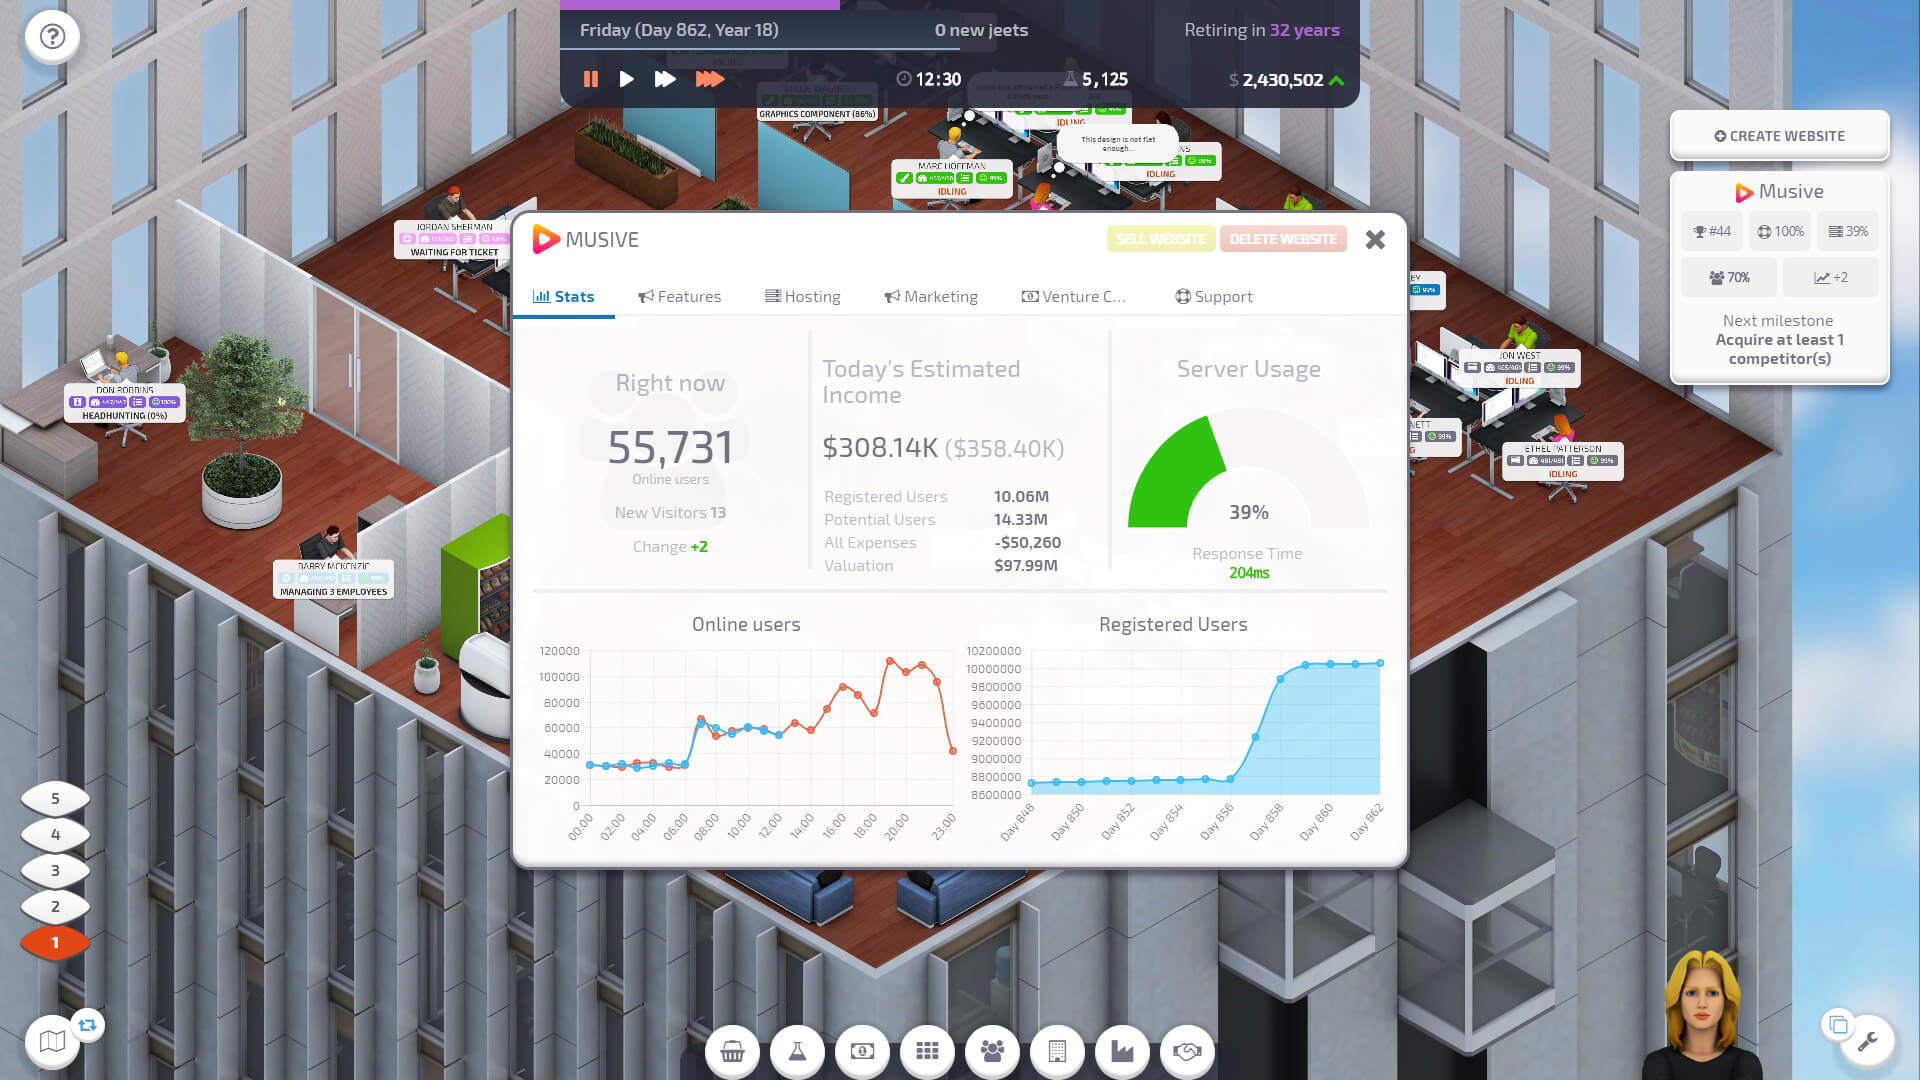
\includegraphics[width=\textwidth]{images/Startup-Metrics.jpg}
    \caption[Startup Company - Métricas que o jogo disponibiliza para o jogador. Retirado de \url{https://store.steampowered.com/app/606800/Startup_Company/?l=portuguese}]{Startup Company - Métricas que o jogo disponibiliza para o jogador.}
    \label{StartUP_Dinheiro}
  \end{minipage}
  \hfill % Espaçamento entre as minipages
  % --- Segunda Figura (Servidores) ---
  \begin{minipage}[b]{0.48\textwidth}
    \centering
    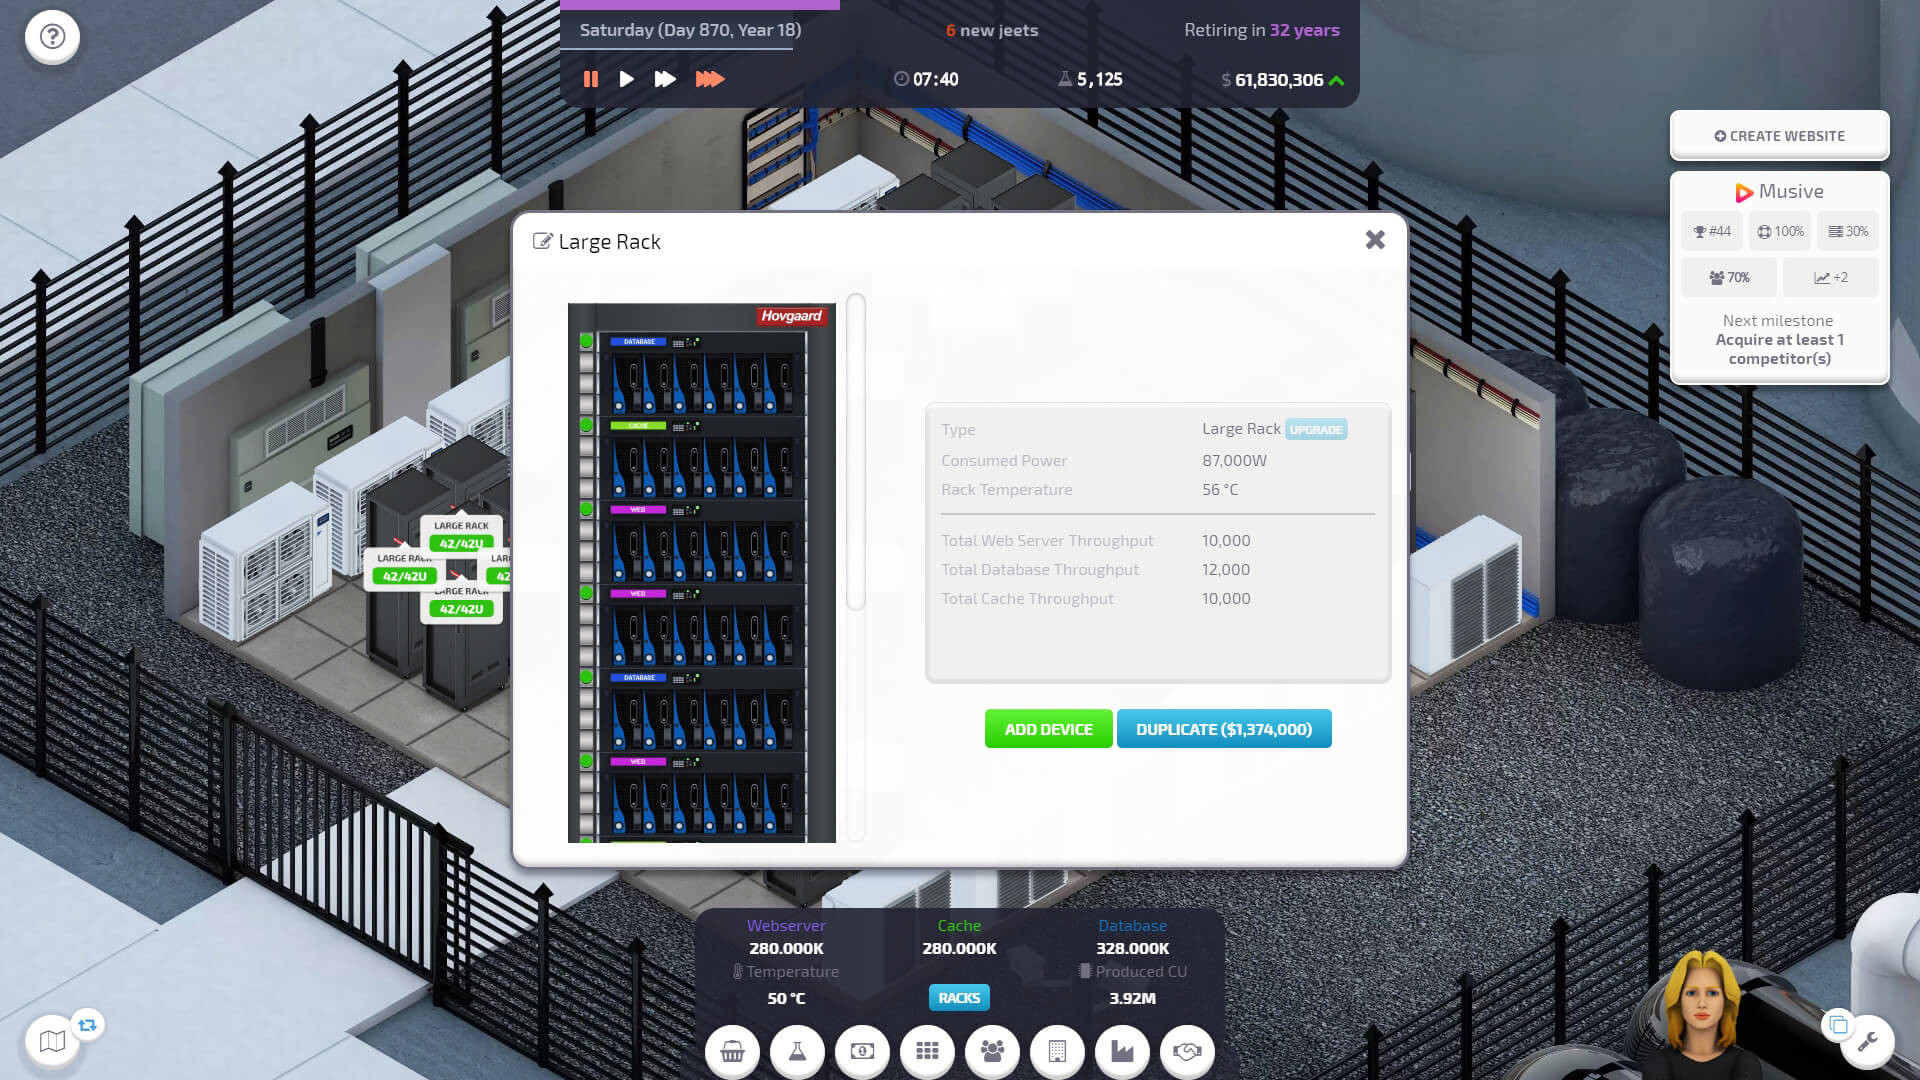
\includegraphics[width=\textwidth]{images/Startup-Server.jpg}
    \caption[Startup Company - Configurações de servidores. Retirado de \url{https://store.steampowered.com/app/606800/Startup_Company/?l=portuguese}]{Startup Company - Configurações de servidores.}
    \label{StarUP_Server}
  \end{minipage}
\end{figure}

\begin{figure}[H]
  \centering
  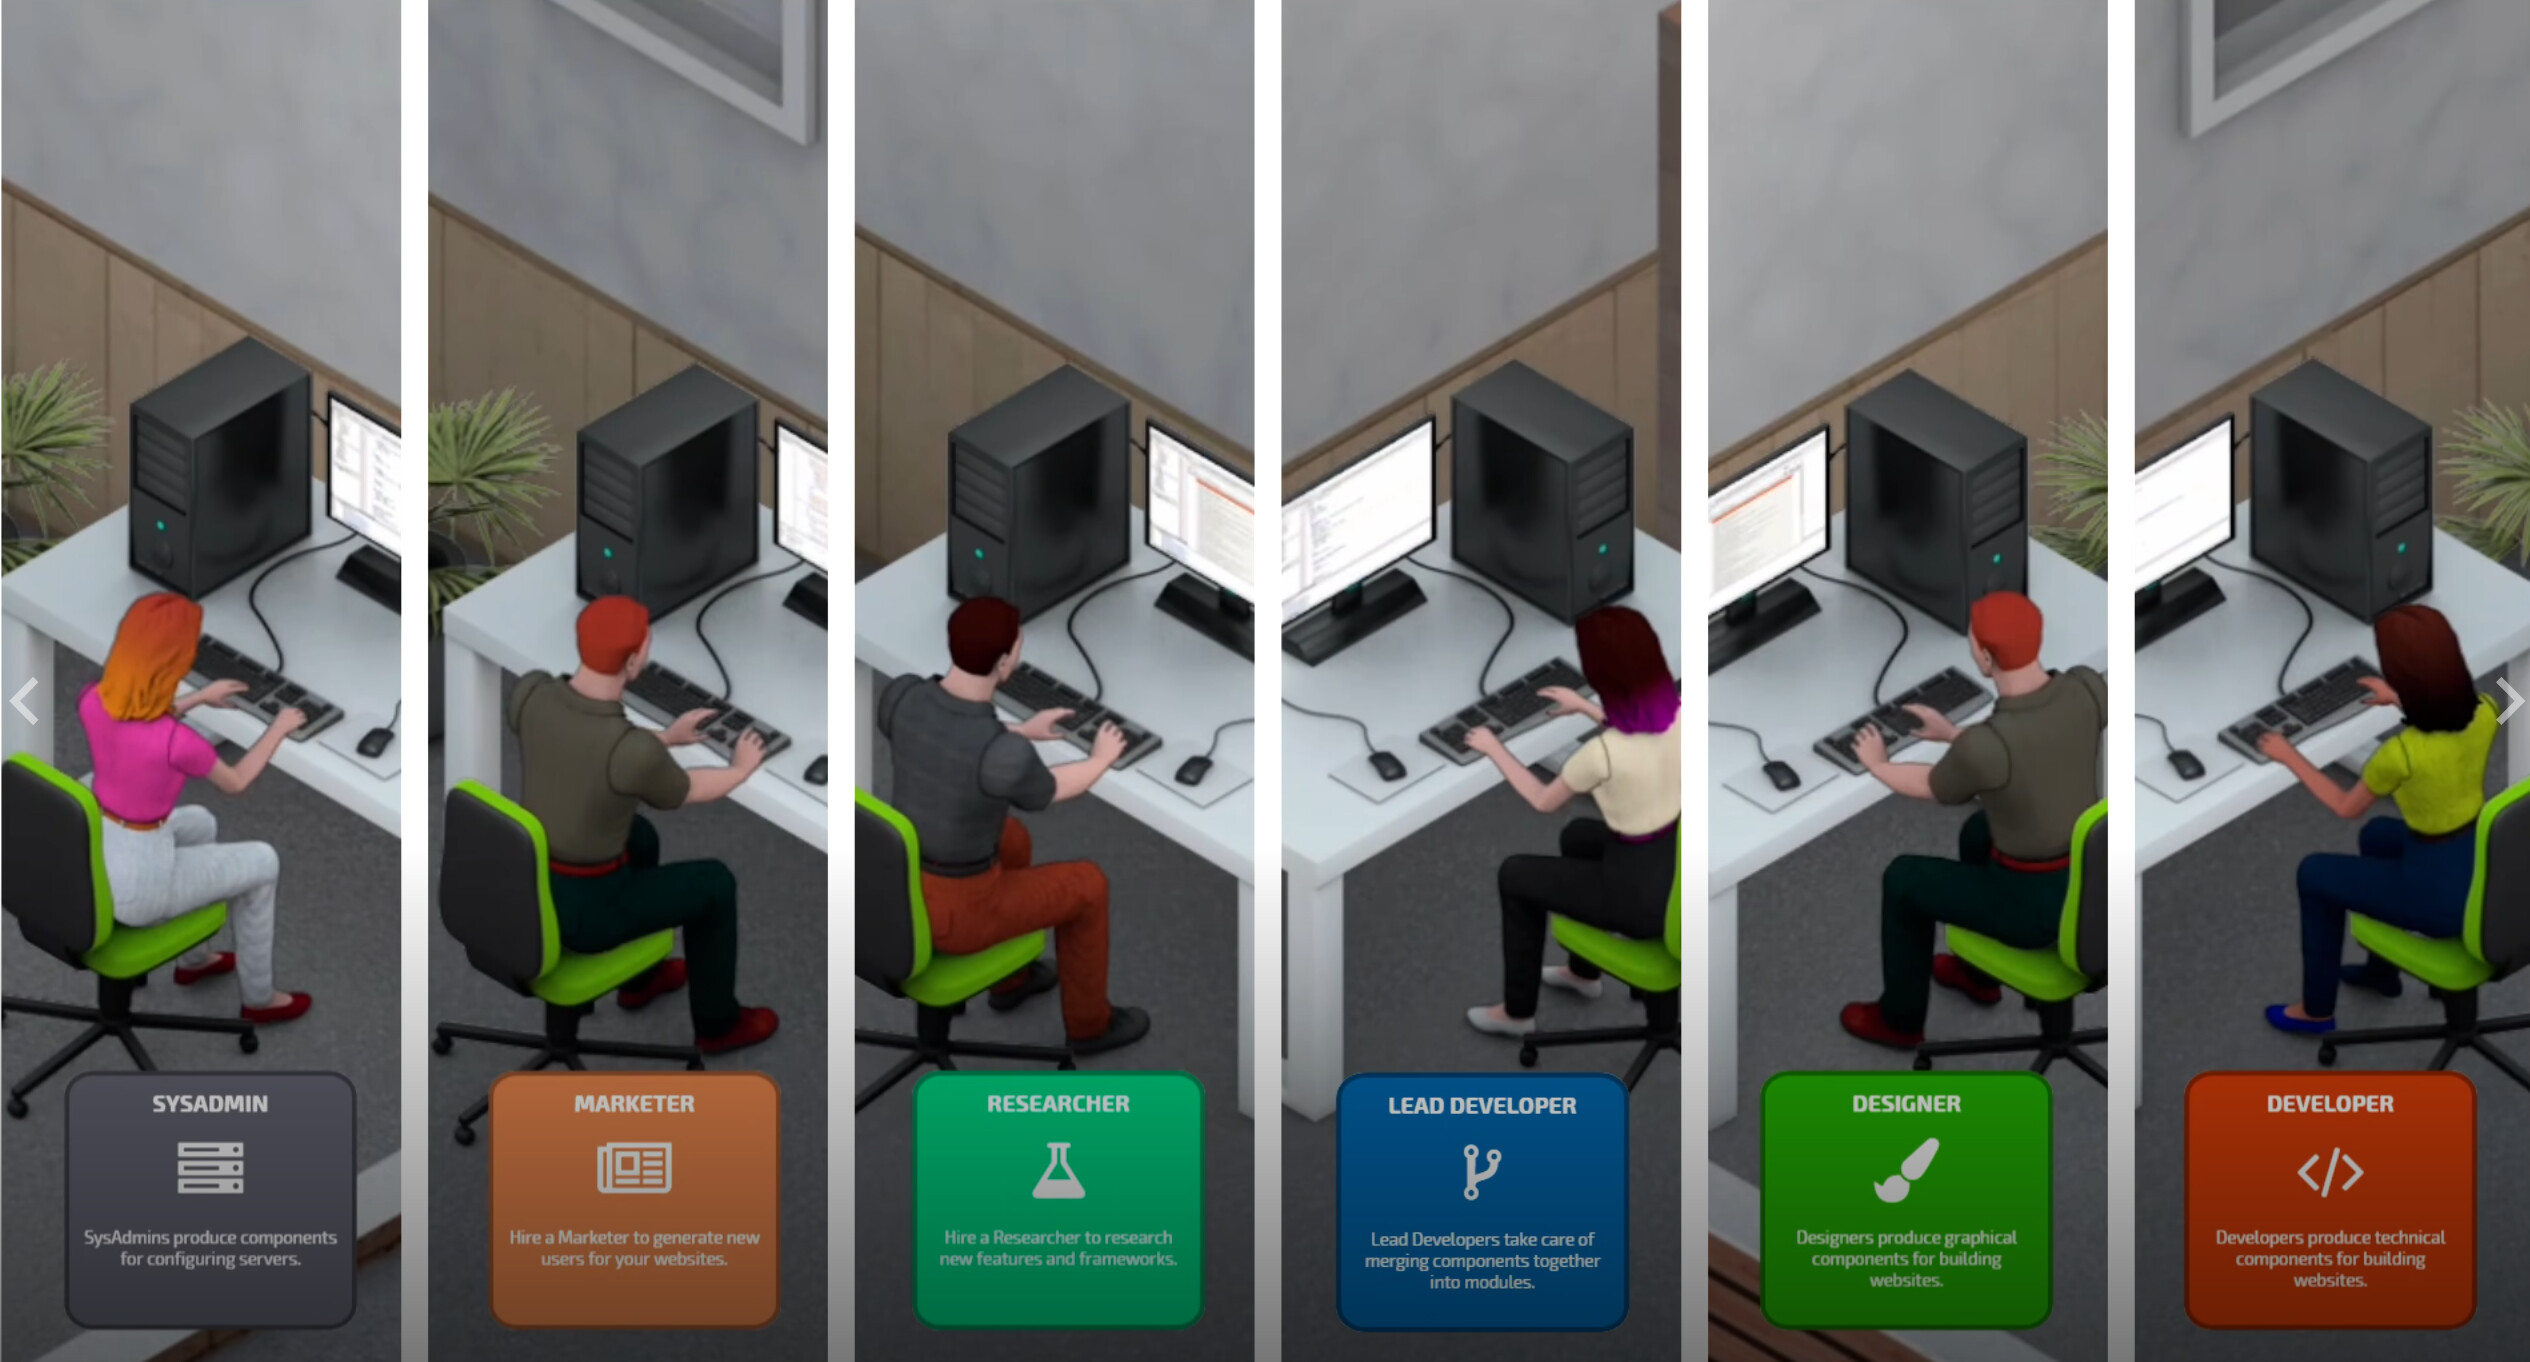
\includegraphics[width=0.6\textwidth]{images/Startu - humanos.jpg}
  \caption[Startup Company - Exemplo de recursos humanos disponiveis. Retirado de \url{https://store.steampowered.com/app/606800/Startup_Company/?l=portuguese}]{Startup Company - Exemplo de recursos humanos disponiveis. Retirado de \url{https://store.steampowered.com/app/606800/Startup_Company/?l=portuguese}}
  \label{StartUP_RH}
\end{figure}

Além dessa parte, gestão de cliente, custo, consumos da infraestrutura assim como rendimentos, são fatores relavantes
neste jogo (ver Figura \ref{StartUP_Dinheiro}). Serviram de inspiração para a criação de funcionalidades no projeto, tais como
pedido de serviços feito por clientes para o jogador, e métricas de consumo e desempenho.


\subsection{Grey Hack}

\begin{figure}[H]
\centering
\begin{tabular}{ll}
\begin{minipage}{0.55\textwidth}
\textcite{GreyHarck} está a desenvolver o jogo Grey Hack (ver Figura \ref{GreyHack_Capa}), o qual está em acesso antecipado na plataforma Steam. Estes títulos focam-se na simulação de ambientes de rede e \textit{hacking} por interfaces que mimetizam sistemas operativos reais , utilizando terminais de linha de comando (CLI).
\end{minipage}
&
\begin{minipage}{0.35\textwidth}
\centering

\includegraphics[width=\textwidth]{images/GreyHack-Header.jpg}
\caption[Grey Hack - Capa do jogo. Retirado de \url{https://store.steampowered.com/app/605230/Grey_Hack}]{Grey Hack - Capa do jogo. }
\label{GreyHack_Capa}
\end{minipage}
\end{tabular}
\end{figure}

Grey Hack utiliza terminais de linha de comando (CLI) e visualizações de 
topologia de rede para criar uma experiência imersiva, onde o jogador interage 
com o sistema de forma lógica e textual (ver Figura \ref{GreyHack_UI}).

\begin{figure}[H]
  \centering
  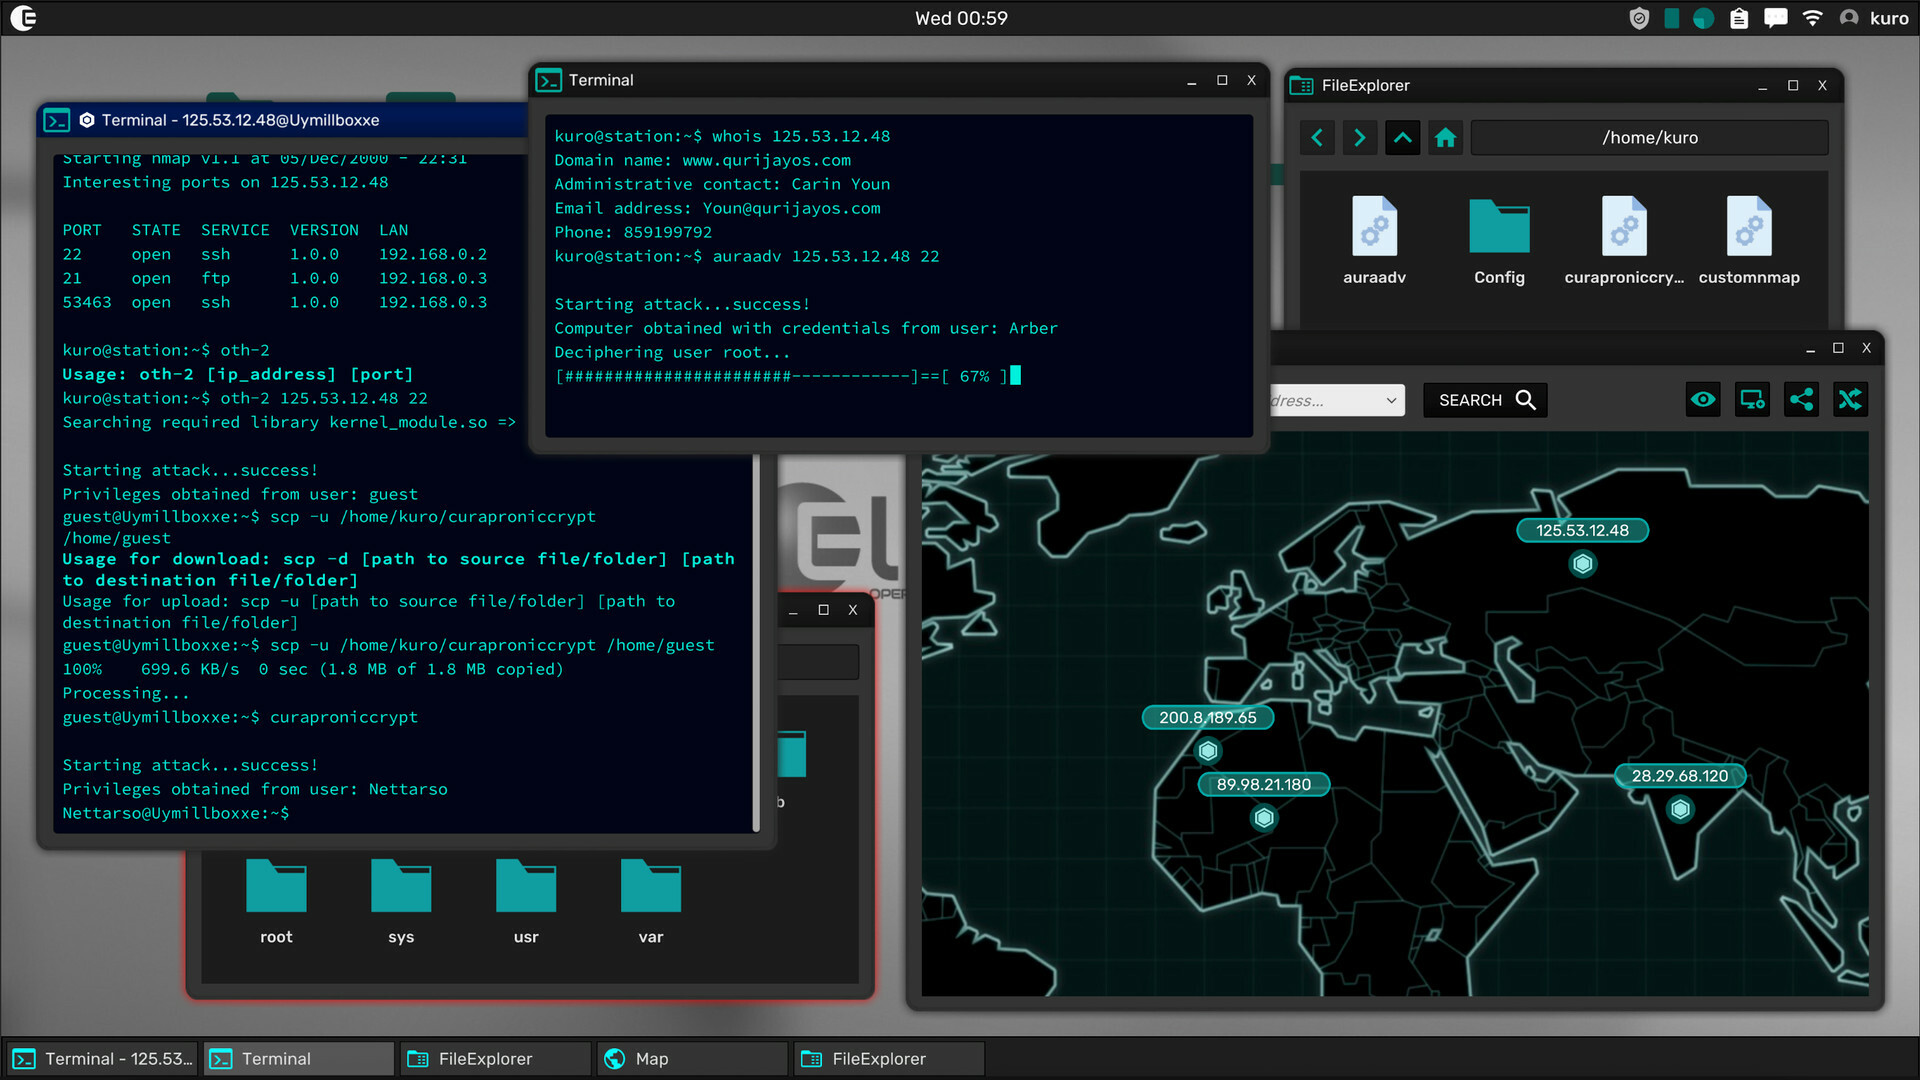
\includegraphics[width=\textwidth]{images/Grey Hack - Terminal.jpg}
  \caption[Grey Hack - UI de terminal. Retirado de \url{https://store.steampowered.com/app/605230/Grey_Hack}]{Grey Hack - UI de terminal. Retirado de \url{https://store.steampowered.com/app/605230/Grey_Hack}}
  \label{GreyHack_UI}
\end{figure}

Transpondo para o projeto, estas referências servem de base para a camada de interação (UI/UX). 
O projeto adota a utilização de terminais virtuais para a conclusão de \textit{mini games}.

\subsection{Software Inc.}

\begin{figure}[H]
\centering
\begin{tabular}{ll}
\begin{minipage}{0.55\textwidth}
\textcite{SoftwareInc} desenvolveu o jogo Software Inc. (ver Figura \ref{SoftwareInc_Capa}), o qual apresenta um sistema de construção complexo que inclui a gestão de eletricidade, temperatura e disposição de salas. O jogo exige que o jogador planeie a colocação de sistemas de arrefecimento e geradores para garantir a integridade do hardware.
\end{minipage}
&
\begin{minipage}{0.35\textwidth}
\centering

\includegraphics[width=\textwidth]{images/SoftwareInc-Header.jpg}
\caption[Software Inc - Capa do jogo. Retirado de \url{https://store.steampowered.com/app/362620/Software_Inc}]{Software Inc - Capa do jogo. }
\label{SoftwareInc_Capa}
\end{minipage}
\end{tabular}
\end{figure}

A influência de Software Inc. no projeto reside no planeamento de sistemas. Tais como a necessidade 
de gerir a gestão da rede elétrica (capacidade das UPS e geradores) são mecânicas de logística urbana adaptadas 
para o ambiente de jogo.

\section{Artigos científicos}
Para além dos videojogos anteriormente referenciados, existe um conjunto de artigos que 
se enquadram na área científica do projeto e que foram fundamentais para sustentar o seu 
desenvolvimento, estabelecendo uma ponte importante entre o universo dos jogos e a aplicação 
real. Um exemplo desta correlação é o trabalho de \textcite{Gametheory-DataCenters}, que demonstra 
como conceitos teóricos complexos, como a Teoria dos Jogos, são aplicados na prática para 
identificar centros de dados vulneráveis em redes de computação em nuvem através da análise 
de custos e tempos de resposta. A inclusão desta referência no estado da arte serve para 
validar como as dinâmicas de gestão e os desafios de infraestrutura abordados no projeto 
refletem preocupações reais e atuais da computação científica, reforçando a relevância 
do contexto em que o utilizador é inserido.

\todo{Revisar}

A metodologia de design é apoiada por \textcite{SeriousGames-Frutuoso}, que descreve diretrizes para a 
criação de jogos com objetivos educacionais. Embora o projeto desenvolvido não se define 
como um jogo sério, a metodologia
 apresentada foi relevante na fase de conceptualização para estruturar a integração de 
 conteúdos técnicos de forma equilibrada. Esta abordagem é complementada pelos conceitos 
 de macrodesign de \textcite{shay2022scaffolding}, que identificam fatores cruciais como a 
 fantasia, o mistério e o desafio para garantir que o rigor do tema não prejudica a imersão 
 lúdica. Para o desenvolvimento deste trabalho, a aplicação destes fatores justifica a 
 inclusão de elementos de fantasia e métricas simplificadas em cima de conhecimentos 
 reais, garantindo que o jogador se mantenha motivado por mecânicas envolventes 
 e permitindo a criação de um conceito de jogo que soma conhecimentos ao jogador mantendo 
 a diversão como fator principal.

Por fim estudo como, \textit{Video Games and Indirect Learning: A Study of 12 Games That Can Teach} realizado
por Monica \textcite{miller2021video} defende que video jogos meramente comerciais, ou
seja jogos que não são focados em transmitir conhecimentos como é o caso de jogos sérios,
 conseguem transmitir conhecemintos ao jogo.

\todo{Aqui}

\chapter{Técnicas e Decisões de Design}

Neste presente capitulo serão explorados os conceitos de design aplicados no projeto
desenvolvido assim como as decisões tomadas durante o processo de desenvolvimento. 
O design do jogo é um elemento crucial para garantir uma experiência envolvente e 
satisfatória para os jogadores, envolve a criação de mecânicas com técnicas de design,
complementa o projeto como um todo.

Serão apresentados métodos científicos e técnicos utilizados para a construção do jogo, 
bem como as escolhas pessoais e criativas que influenciaram o desenvolvimento do projeto. 
O objetivo é estabelecer uma compreensão clara do processo de design e das decisões tomadas.

\section{Técnicas utilizadas}

Nas subsecção consequentes serão descritas e apresentadas as técnicas de design utilizadas no desenvolvimento do projeto,
incluindo a aplicação de princípios de design e metodologias de desenvolvimento.

\subsection{\textit{Framework} MDA (\textit{Mechanics, Dynamics, Aesthetics})}

O \textit{framework} MDA, desenvolvido por \textcite{framework-mda}, é uma abordagem amplamente 
utilizada no design de jogos concentrados em três componentes 
principais: Mecânicas, Dinâmicas e Estéticas.
As Mecânicas referem-se às regras e sistemas que governam o jogo, 
as Dinâmicas são as interações inerentes entre as mecânicas e os jogadores, 
e as Estéticas são as emoções e experiências que os jogadores vivenciam ao jogar.

Posto isto, o \textit{framework} MDA foi utilizado como guia para a construção do jogo,
e o diagrama apresentado na Figura \ref{MDA_Diagram} ilustra a relação entre as mecânicas, dinâmicas e estéticas do jogo desenvolvido.

\begin{figure}[h!]
    \centering
    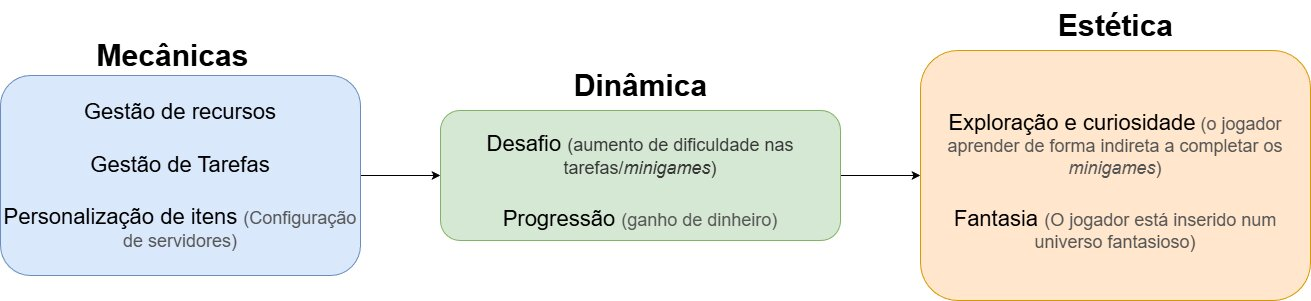
\includegraphics[width=1\textwidth]{Diagramas/MDA.jpg}
    \caption{Diagrama do \textit{framework} MDA aplicado ao jogo desenvolvido.}
    \label{MDA_Diagram}
\end{figure}

\subsection{\textit{Flow}}


Embora venha da psicologia, o trabalho de \textcite{flow} é a base para o design de 
progressão em jogos. Define o equilíbrio entre a dificuldade do desafio e a habilidade do jogador para evitar o tédio ou a ansiedade.
O conceito de \textit{Flow} foi aplicado no design do jogo para garantir que os 
jogadores se mantenham engajados e motivados a continuar jogando, 
proporcionando desafios adequados ao nível de habilidade dos jogadores.

Na Figura \ref{Flow_Diagram} é possível observar um diagrama que ilustra o conceito de \textit{Flow} aplicado ao design do jogo.

\begin{figure}[h!]
    \centering
    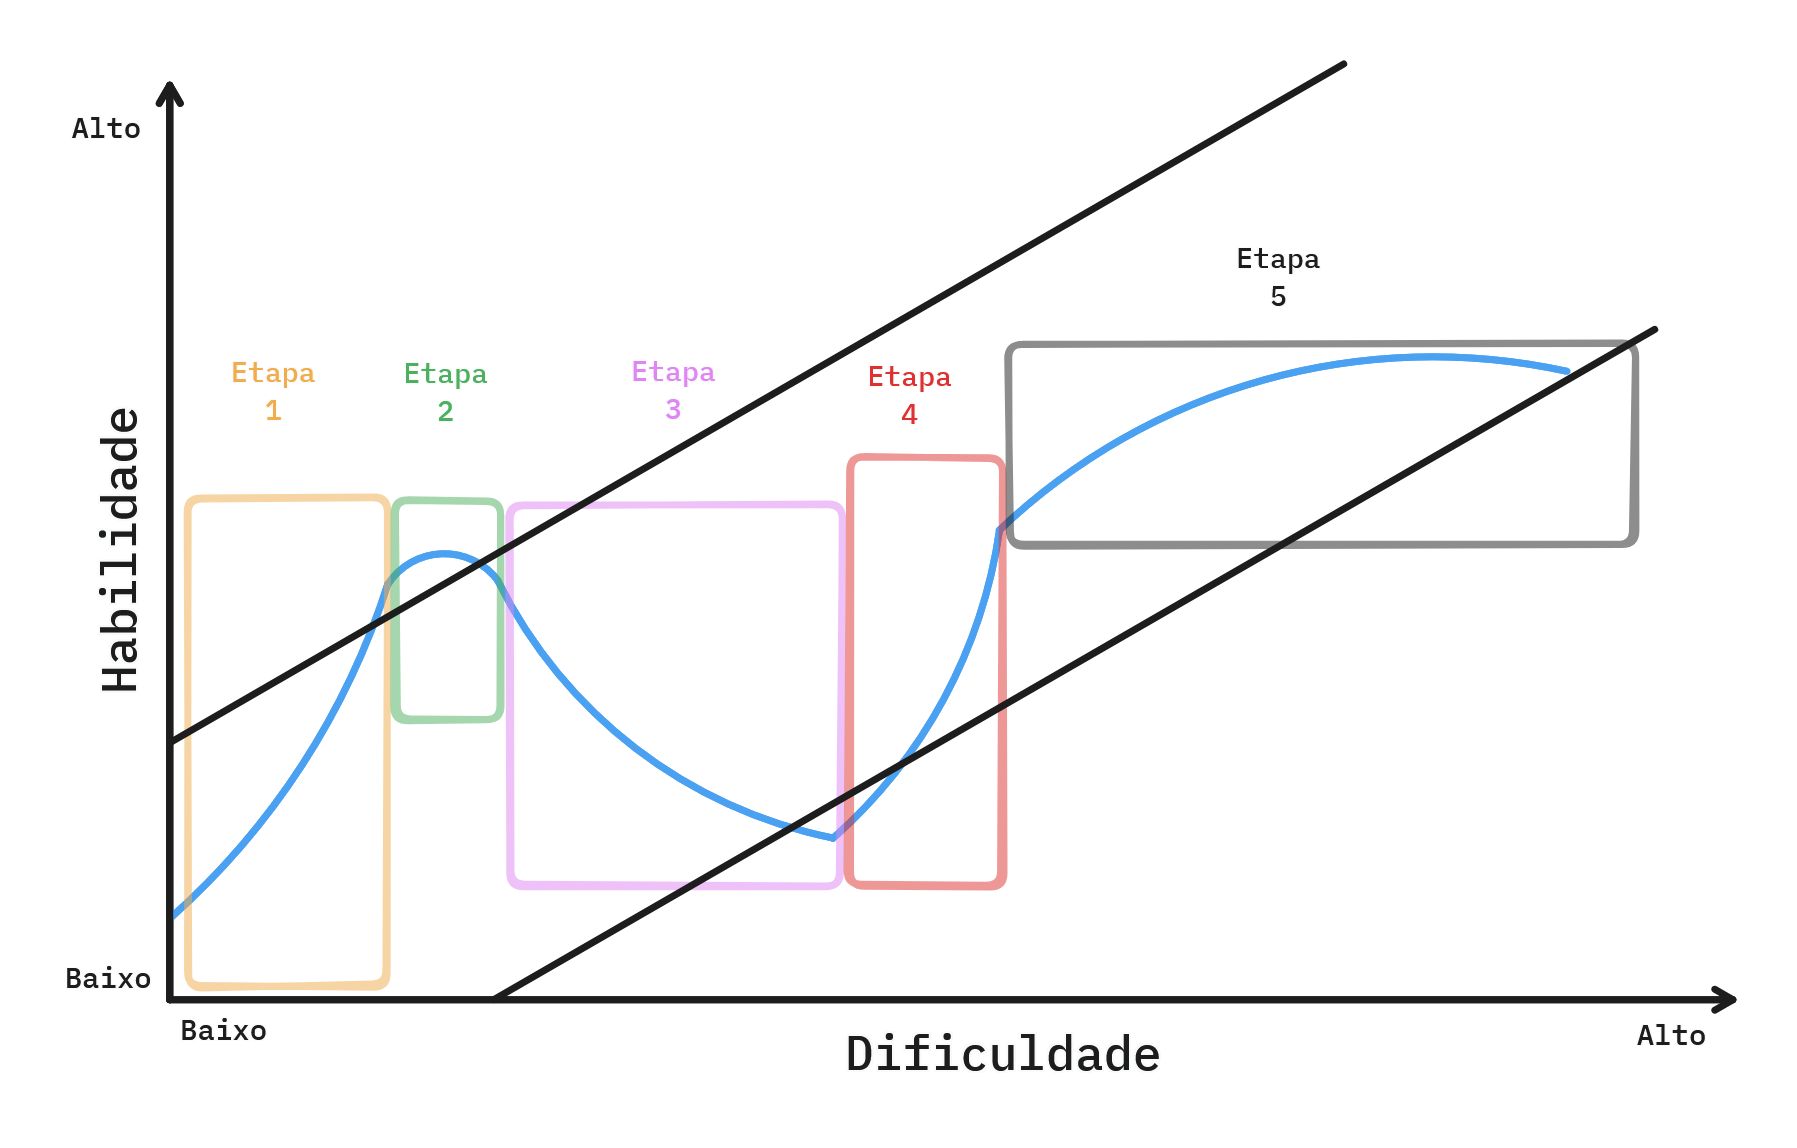
\includegraphics[width=0.5\textwidth]{Diagramas/Flow Graph.png}
    \caption{Diagrama do conceito de \textit{Flow} aplicado ao design do jogo.}
    \label{Flow_Diagram}
\end{figure}

O diagrama é divido em 5 etapas, onde cada uma dela representam momentos específicos do jogo.
A 1º etapa representa os primeiros momentos do jogo, onde o jogador está a aprender as mecânicas básicas
e a preceber o que tem de fazer para progredir, como tal é representa por uma curva crescente.

A 2º etapa é caracterizada pela adptação do jogador às mecânicas introduzidas na etapa anterior,
como tal a curva de \textit{flow} começa a descer, uma vez que devida a adaptação do jogador, o desafio se torna mais fácil.

A 3º etapa representa a habituação do jogador às mecânicas, assim como a repetição de desafios semelhantes,
o que leva a uma curva de \textit{flow} com um declive negativo, uma vez que o jogador começa
a sentir-se entediado e desmotivado a continuar jogando.

A 4º etapa, por contraste com a anterior, é caracterizada pela introdução de inimigos, o que indiretamente implica a introção de
mecânicas novas e quebra o ciclo até aquele momento, o que leva a um aumento da dificuldade percebila pelo
jogador, o que indiretamente justifica o aumento do \textit{flow}.

Por fim a 5º etapa é caracterizada por uma adaptação, da parte do jogador, às
mecânicas introduzidas na etapa anterior, com as mecânicas iniciais,
o que resulta numa curva de \textit{flow} com um crescimento bastante moderado, uma vez que o
jogador já tem uma base sólida construida com as mecânicas anteriores, 
o que o torna a \textit{gameplay} muito mais previsível, resultando assim numa 
curva de \textit{flow} mais estável e menos propensa a declives acentuados.

Em suma, a progressão do jogo utiliza a alternância entre a introdução de novos 
desafios e períodos de adaptação para modular a experiência do utilizador. Ao gerir 
estas cinco etapas, o design garante que o jogador no estado de \textit{Flow}, 
equilibrando a curva de aprendizagem com momentos de novidade, assegurando assim uma 
experiência envolvente, fluida e recompensadora do início ao fim.

\subsection{Modelo de \textit{Hook}}

No âmbito do game design contemporâneo e do desenvolvimento de produtos digitais, a 
retenção de utilizadores tornou-se um dos indicadores de desempenho mais críticos. 
Neste contexto, o Modelo de Hook \textit{(Hook Model)}, conceptualizado por \textcite{modelo_hook}, 
surge como uma estrutura teórica e prática desenhada para fomentar a criação de 
hábitos através da interação contínua com o produto.

Ao contrário de abordagens baseadas meramente em publicidade agressiva, o Modelo de 
Hook foca-se na psicologia do utilizador, ligando os seus problemas e necessidades 
quotidianas a uma solução tecnológica específica. Este modelo é composto por um ciclo 
iterativo de quatro fases fundamentais: o Gatilho \textit{(Trigger)}, a Ação \textit{(Action)}, a 
Recompensa Variável \textit{(Variable Reward)} e o Investimento \textit{(Investment)}.

Posto isto, o Modelo de Hook utilizado no desenvolvimento deste projeto, é caracterizado
pelos seguintes elementos:

\begin{itemize}
    \item \textit{Trigger}: Curiosidade pela temática do jogo, apelo pelo visual e apelo de curiosidade pelo uso de técnicas e tecnologias reais, senso de colecionismo. Retornar ao jogo para obter o dinheiro que está em estado pendente.
    \item \textit{Ação}: Resolução de puzzles rápidos, cerca de 60 segundos, sobre a forma de \textit{minigames}, otimização de recursos e processos. Derrotar inimigos e fazer melhoramentos gerais.
    \item \textit{Recompensas}: Obtenção de novos recursos, equipamentos e troféus, (colecionismo), melhoramento de equipamentos.
    \item \textit{Investimento}: Investimento de tempo e esforço para a progressão no jogo.
\end{itemize}

Alguns elementos presente no modelo assim, como troféus e melhoramento de equipamentos (tanto 
de servidores como de armas), estão presente no conceito de design do jogo, no entanto,
não estão contenplados no projeto desenvolvido, uma vez que não eram o foco principal e
não existiu tempo suficiente para a sua implementação.

\section{Decisões de Design}

\subsection{\ac{UI} e referências técnicas}

A \textit{User Interface} (\ac{UI}) do jogo está presente durante toda a \textit{gameplay},
como tal construir uma \ac{UI} clara e que se enquadre no contexto do jogo, é de suma importância.
Essa visão é partilhado por \textcite{adams_fundamentals} que argumenta que a \ac{UI} deve 
atuar como uma "extensão do mundo" através do seu estilo visual.

Assim, a \ac{UI} do jogo é inspirada no estilo de programas com interfaces de \textit{Command Line Interface} (\ac{CLI}), 
com um design minimalista e funcional, utilizando cores escuras e elementos 
visuais que remetem para o contexto de Data Center, como, por exemplo, gráficos 
de barras para representar o uso de recursos, ou ícones de servidores para 
representar os equipamentos disponíveis.

\begin{figure}[H]
    \centering
    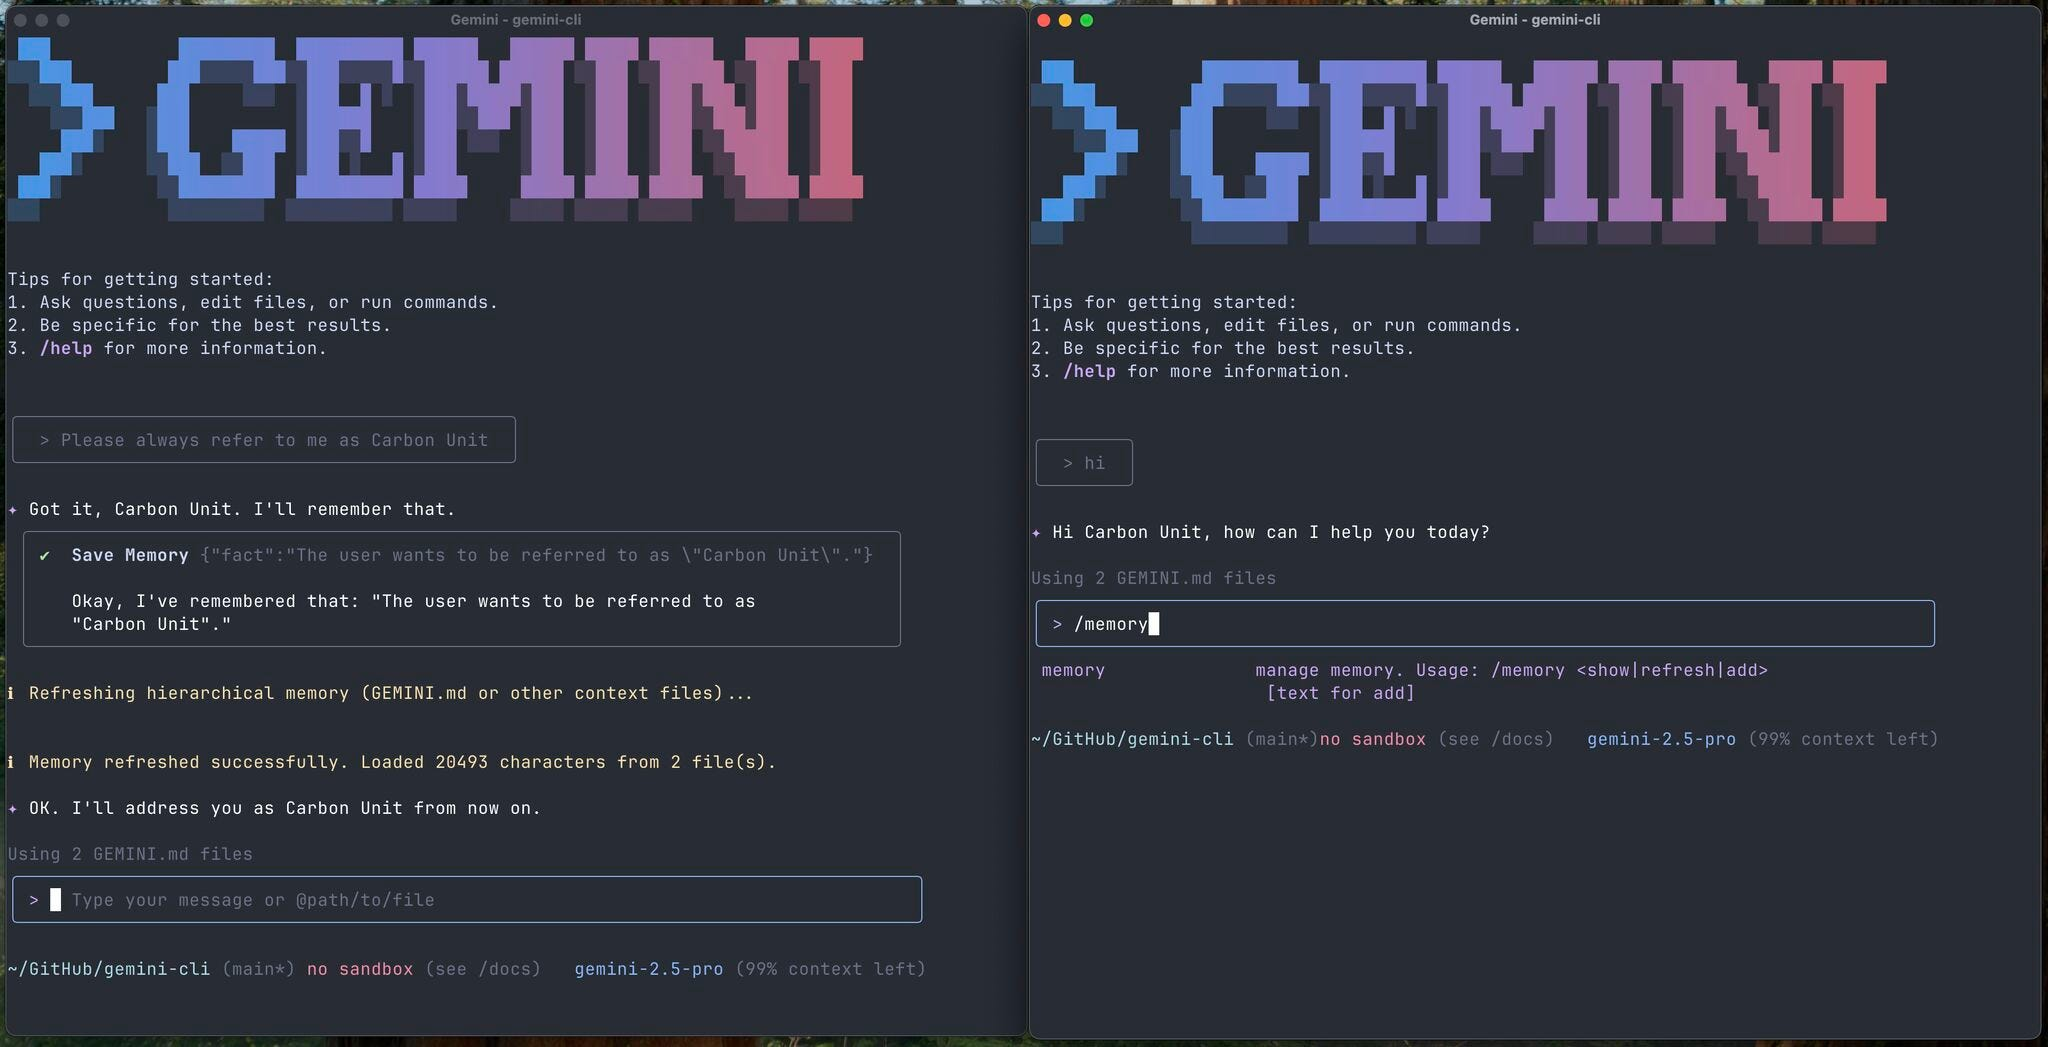
\includegraphics[width=0.8\textwidth]{images/CLI - GEMINI UI.jpg}
    \caption{Exemplo de referência - \ac{UI} do Gemini utilizado em \ac{CLI}}
    \label{UI_Gemini}
\end{figure}

\begin{figure}[H]
    \centering
    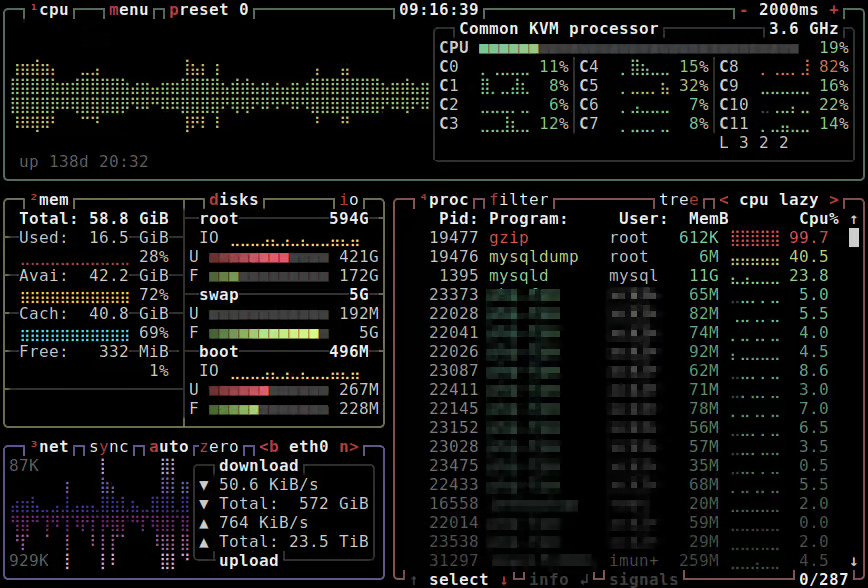
\includegraphics[width=0.8\textwidth]{images/CLI - btop UI.jpg}
    \caption{Exemplo de referência - \ac{UI} do btop}
    \label{UI_BTOP}
\end{figure}

As Figuras \ref{UI_Gemini} e \ref{UI_BTOP} apresentam exemplos de referências utilizadas 
para a construção da \ac{UI} do jogo.
A \ac{UI} das referências apresentadas é caracterizada pelo uso de cores escuras de fundo,
o uso de fonte mono espaçadas, e o uso de gráficos simples, geralmente composto, por
barras, pontos, linhas, caracteres ou quadrados.

Esses mesmos elementos podem ser visto da \ac{UI} da loja, por exemplo, (Figura \ref{Projeto_config_cpu1})
onde é utilizada uma cor de fundo escura, o uso da fonte JetBrains Mono, que é uma fonte mono espaçada,
o uso de texto e o uso de gráficos simples, como os botões e as barras de \textit{status}.

\subsection{Design de Level}

O design de level é o ato de projetar os níveis de um jogo, incluindo a 
disposição dos elementos, a criação de desafios e a definição do 
ritmo do jogo. Como tal é um dos pontos mais críticos para a construção de um jogo, uma vez
que interfere diretamente na experiência e ritmo percebido pelo jogador.

Posto isto o design de level do jogo foi desenvolvido para ser compacto,
mas que, ao mesmo tempo, cada área ofereça uma experiência distinta, que está diretamente
relacionada com a curva de \textit{flow} recebido pelo jogador.

\begin{figure}[H]
    \centering
    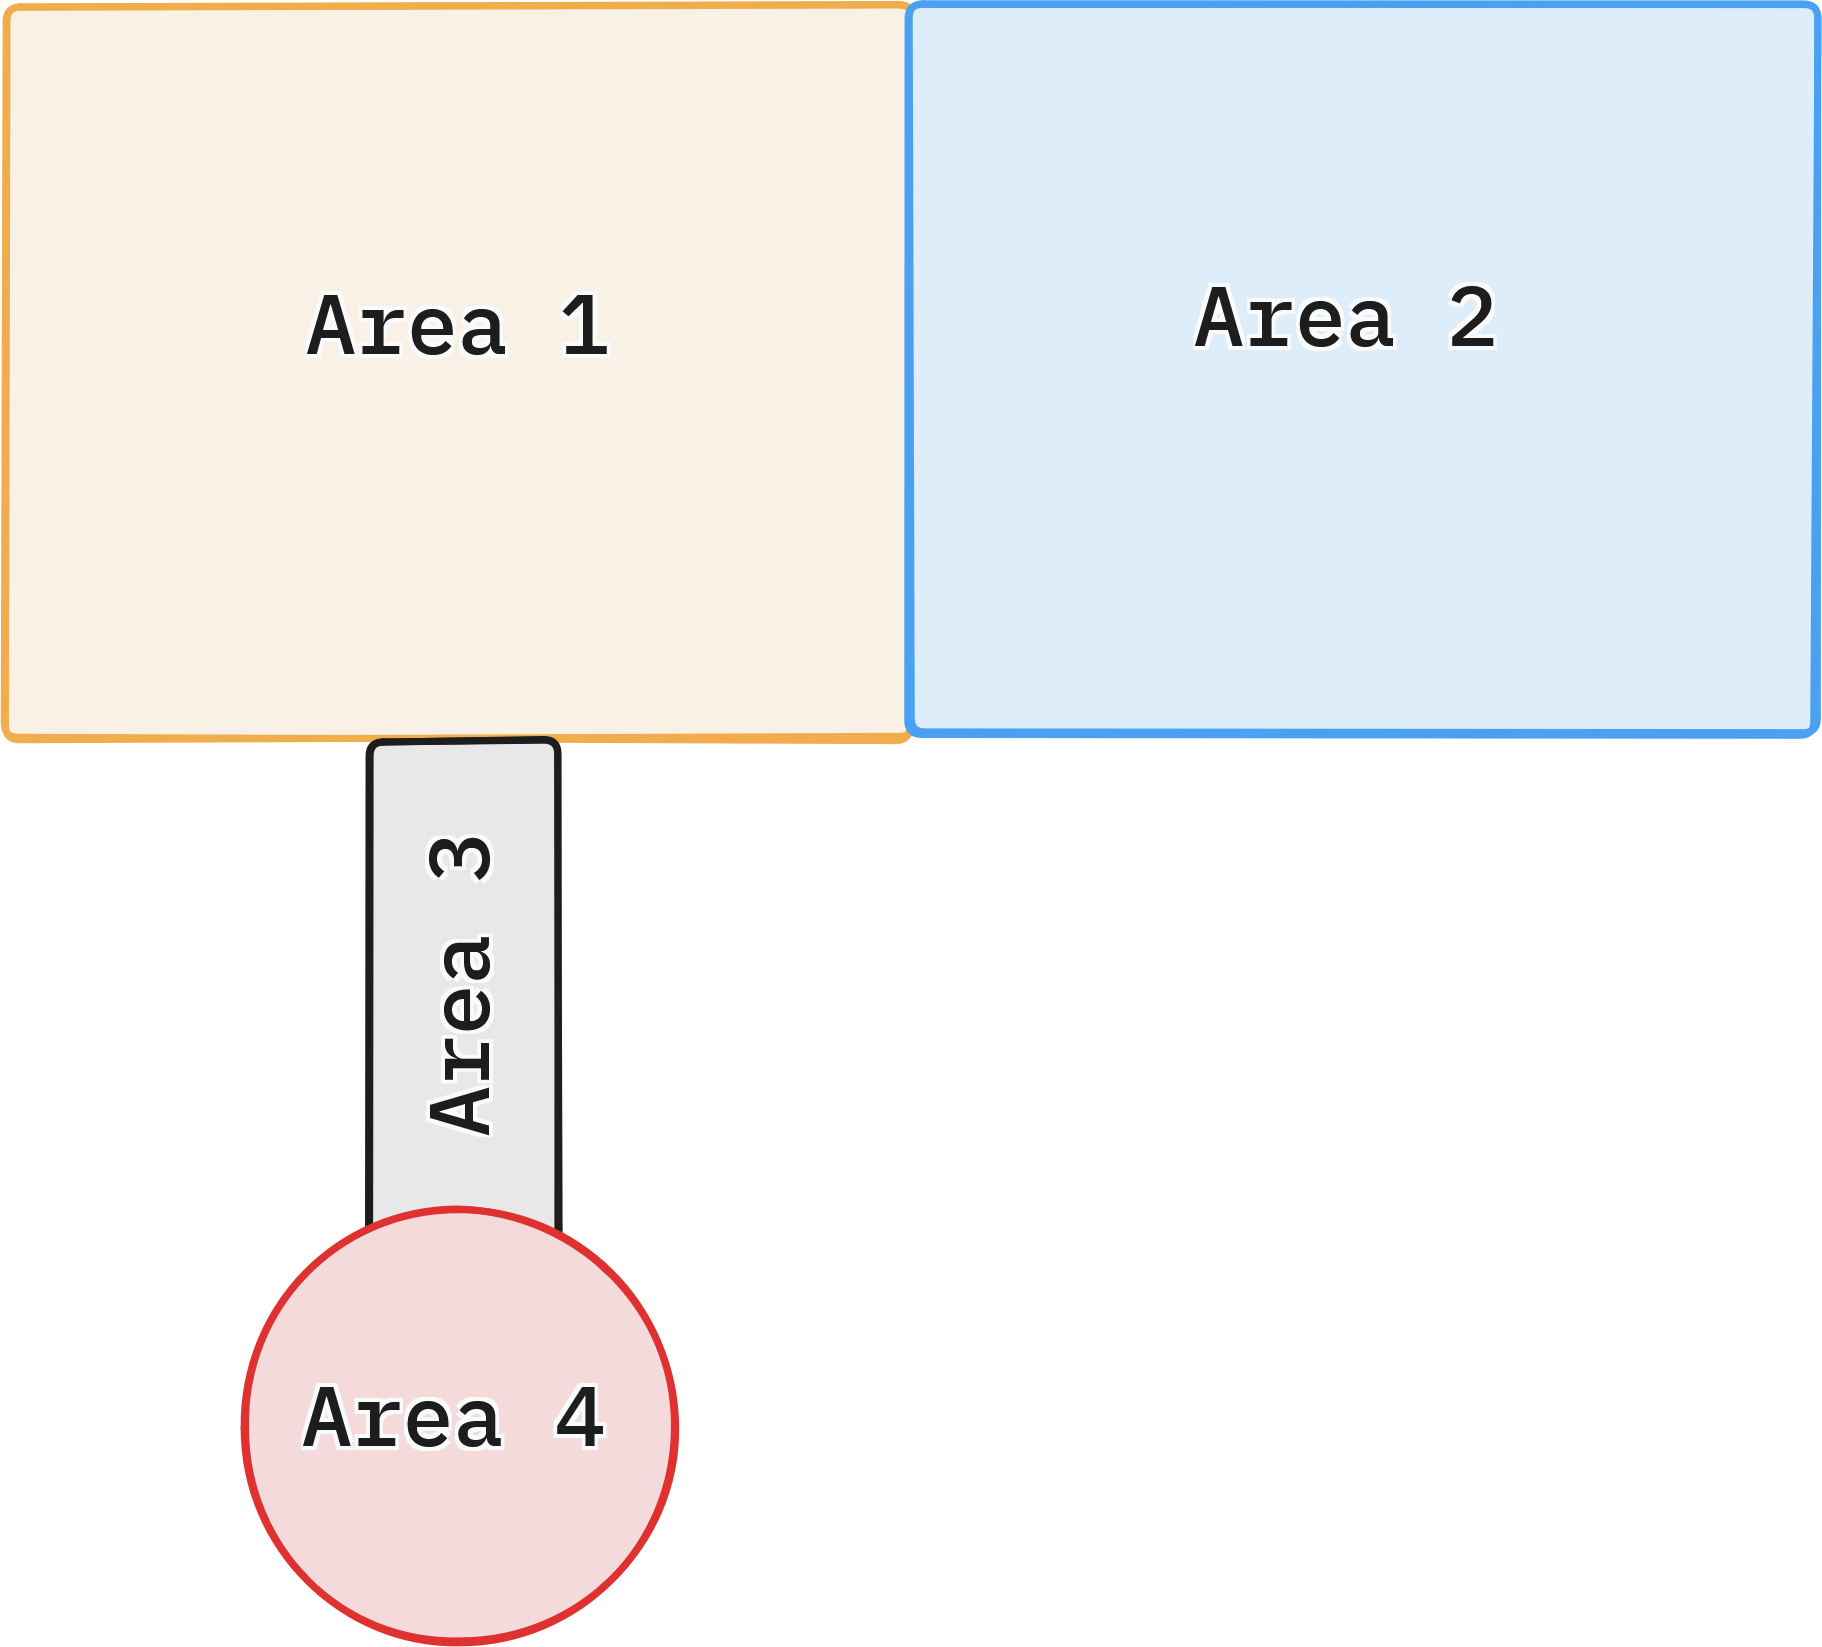
\includegraphics[width=0.8\textwidth]{Diagramas/Level Design.png}
    \caption{Level design do jogo desenvolvido.}
    \label{Level_Design}
\end{figure}

Na Figura \ref{Level_Design} está representado o design do level do jogo divido em
4 áreas distintas, sendo que cada uma tem as seguintes características:
\begin{itemize}
    \item Área 1: Área principal, onde estão localizados os servidores, e onde o jogador interage com os mesmo para resolver os puzzles, que dão dinheiro como recompensa para o jogador. É nesta área onde o jogador irá passar a maior parte do tempo, e por isso mesmo é que é a área central e a área que serve de união para as outras duas.
    \item Área 2: Área de conquista e customização, nessa área o jogador poder ver conquistas obtidas sobre a forma de troféus ou objetos de jogo. Além disso nesta área o jogador poderá interagir com o cenário para o costumizar, como por exemplo interraguir com um computador ou aparelho para fazer upgrades no cenário ou costumizar cores, etc... Esta área é caracterizada por ser um espaço de relaxamento, sem objetivos nem inimigos.
    \item Área 3: É um corredor que liga a área 1 à área 4. Não tem nenhum objetivo primário.
    \item Área 4: Área de combate, nessa área o jogador terá de utilizar de uma metralhadora para derrotar conjuntos de inimigos que irão atacar o data center. Esta área é muito especial pois é nela que existe o rompimento da \textit{gameplay}, e por isso mesmo a necessidade da existência da área 3, uma vez que o corredor representa o distânciamento do conforto proporcionado pelos puzzle da área 1. O formato geométrico dessa área também ajuda a transmitir esse contraste, uma vez que enquanto todas as outras áreas apresentam um formato quadrado, esta área apresenta um formato circular. O formato quadrado geralmente está associado a algo estável, sélido e imóvel, enquanto que o formato circular está associado a algo fluido móvel e instável. Assim, o formato circular representa a mudança de mentalidade que o jogador têm de ter, pois nessa área o jogador terá de ser rápido e capaz de desenvolver uma \textit{gameplay} dinâmica, que o combate exige. Além disso a distância geométrica entre a área 4 e área 2, é a maior de todas estando em pontas opostas, o que ajudar a transmitar a ideia de algo caótico, uma vez que a área 2 é um espaço de relaxamento.
\end{itemize}

Todavia no projeto apresentado, a área 2 não foi implementada na sua totalidade, devido a sua complexidade,
sobre tudo pela parte de desenvolvimento de troféus e pela parte de customização de cenário.

\subsection{Notificações}

Durante o desenvolvimento do jogo surgir a necessidade de desenvolver um sistema
capaz de transmitir \textit{feedbacks} informativos para o jogador. Como, por exemplo,
notificar o jogador quando é realizada com compra, completada uma tarefa, destruído um servidor, etc ...

Segundo \textcite{notificações}, o uso de notificações em jogos, é recomendável e
apresenta um efeito positivo no desempenho do jogador.

Para suprir essa necessidade foi desenvolvido um simples sistema de notificações.
O sistema envia uma notificação, sobre a forma de texto, ao jogador, sempre que acontece, alguma
das ações descritas acima.

\begin{figure}[H]
    \centering
    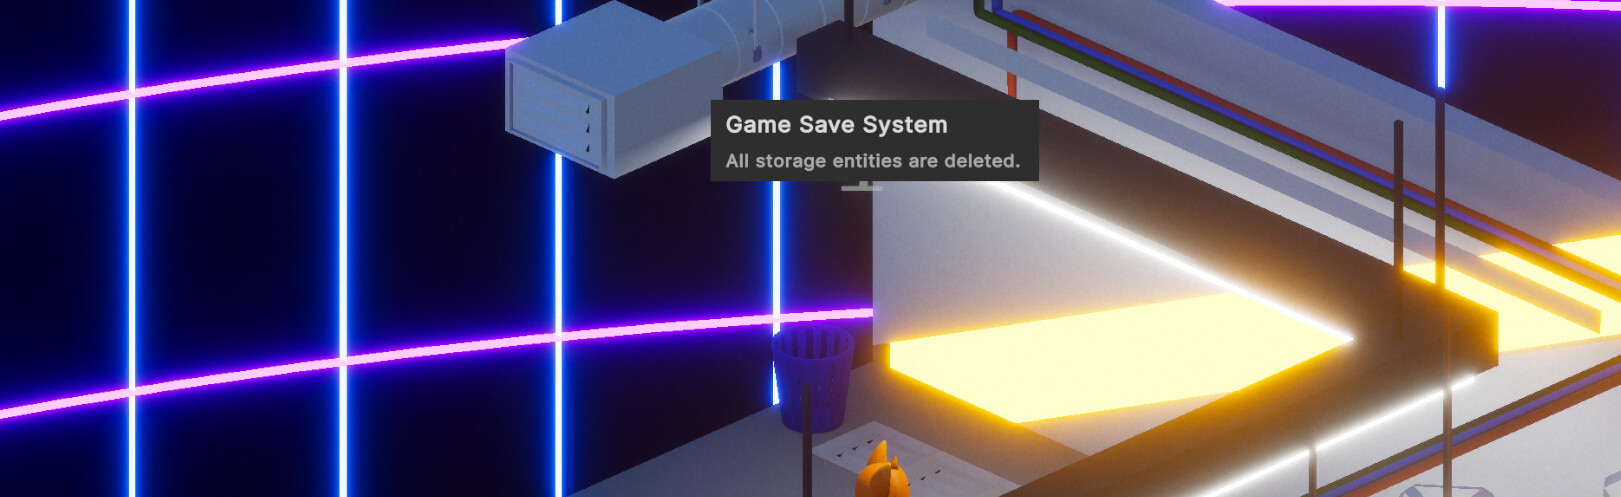
\includegraphics[width=0.8\textwidth]{images/Notificação 1.jpg}
    \caption{Notificação - Destruir todos os servidores.}
    \label{Notificacao_1}
\end{figure}

\begin{figure}[H]
    \centering
    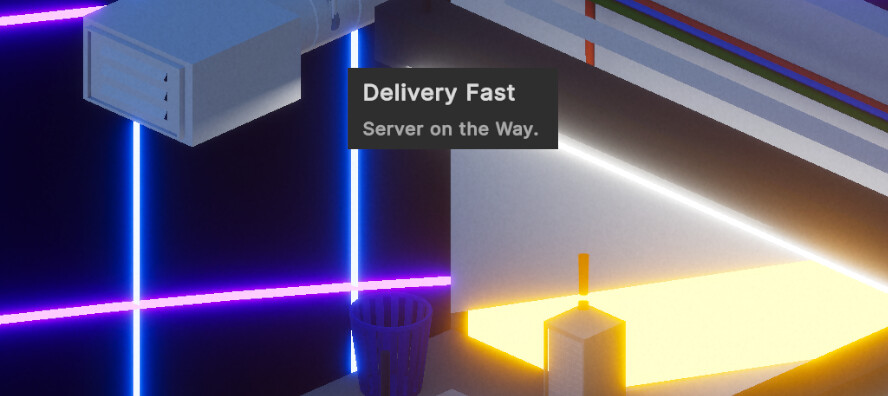
\includegraphics[width=0.8\textwidth]{images/Notificações 2.jpg}
    \caption{Notificação - Compra de um novo servidor.}
    \label{Notificacao_2}
\end{figure}

As Figuras \ref{Notificacao_1} e \ref{Notificacao_2} exemplificação como as notificações são
executadas durante o ciclo de \textit{gameplay}.

\subsection{Referências para a criação de elementos de Jogo e 3D}

No processo de criação de elementos de jogo, sobretudo elementos 3D de cenário, houve o cuidado de utilizar referências reais, como por exemplo, fotos de data centers reais, para a construção dos elementos do jogo, no sentido de criar uma experiência mais imersiva para o jogador, além de possibilitar a criação de conexões entre o jogo e o mundo real, o que se torna benéfico para a construção de uma experiência mais lúdica além de facilitar conexões entre o jogo e jogadores que tenham interesse na temática do jogo, ou que tenham experiência prévia.

No entanto, houve uma adaptação dos mesmos, e uma adição de elementos de fantasia, para criar um ambiente mais divertido e envolvente para o jogador, além de proporcionar uma experiência mais dinâmica e variada.

Neste sentido, houve uma pesquisa prévia sobre a estrutura física de um data center, o que resultou num conjunto de elementos de cenário, que são bastante específicos, destes ambientes. Tais como:
\begin{itemize}
    \item Pavimento técnico;
    \item Racks de servidores;
    \item Cabos de rede;
    \item Sistemas de refrigeração;
    \item Geradores de energia;
    \item Equipamentos de rede;
\end{itemize}

\begin{figure}[H]
    \centering
    \begin{minipage}{0.48\textwidth}
        \centering
        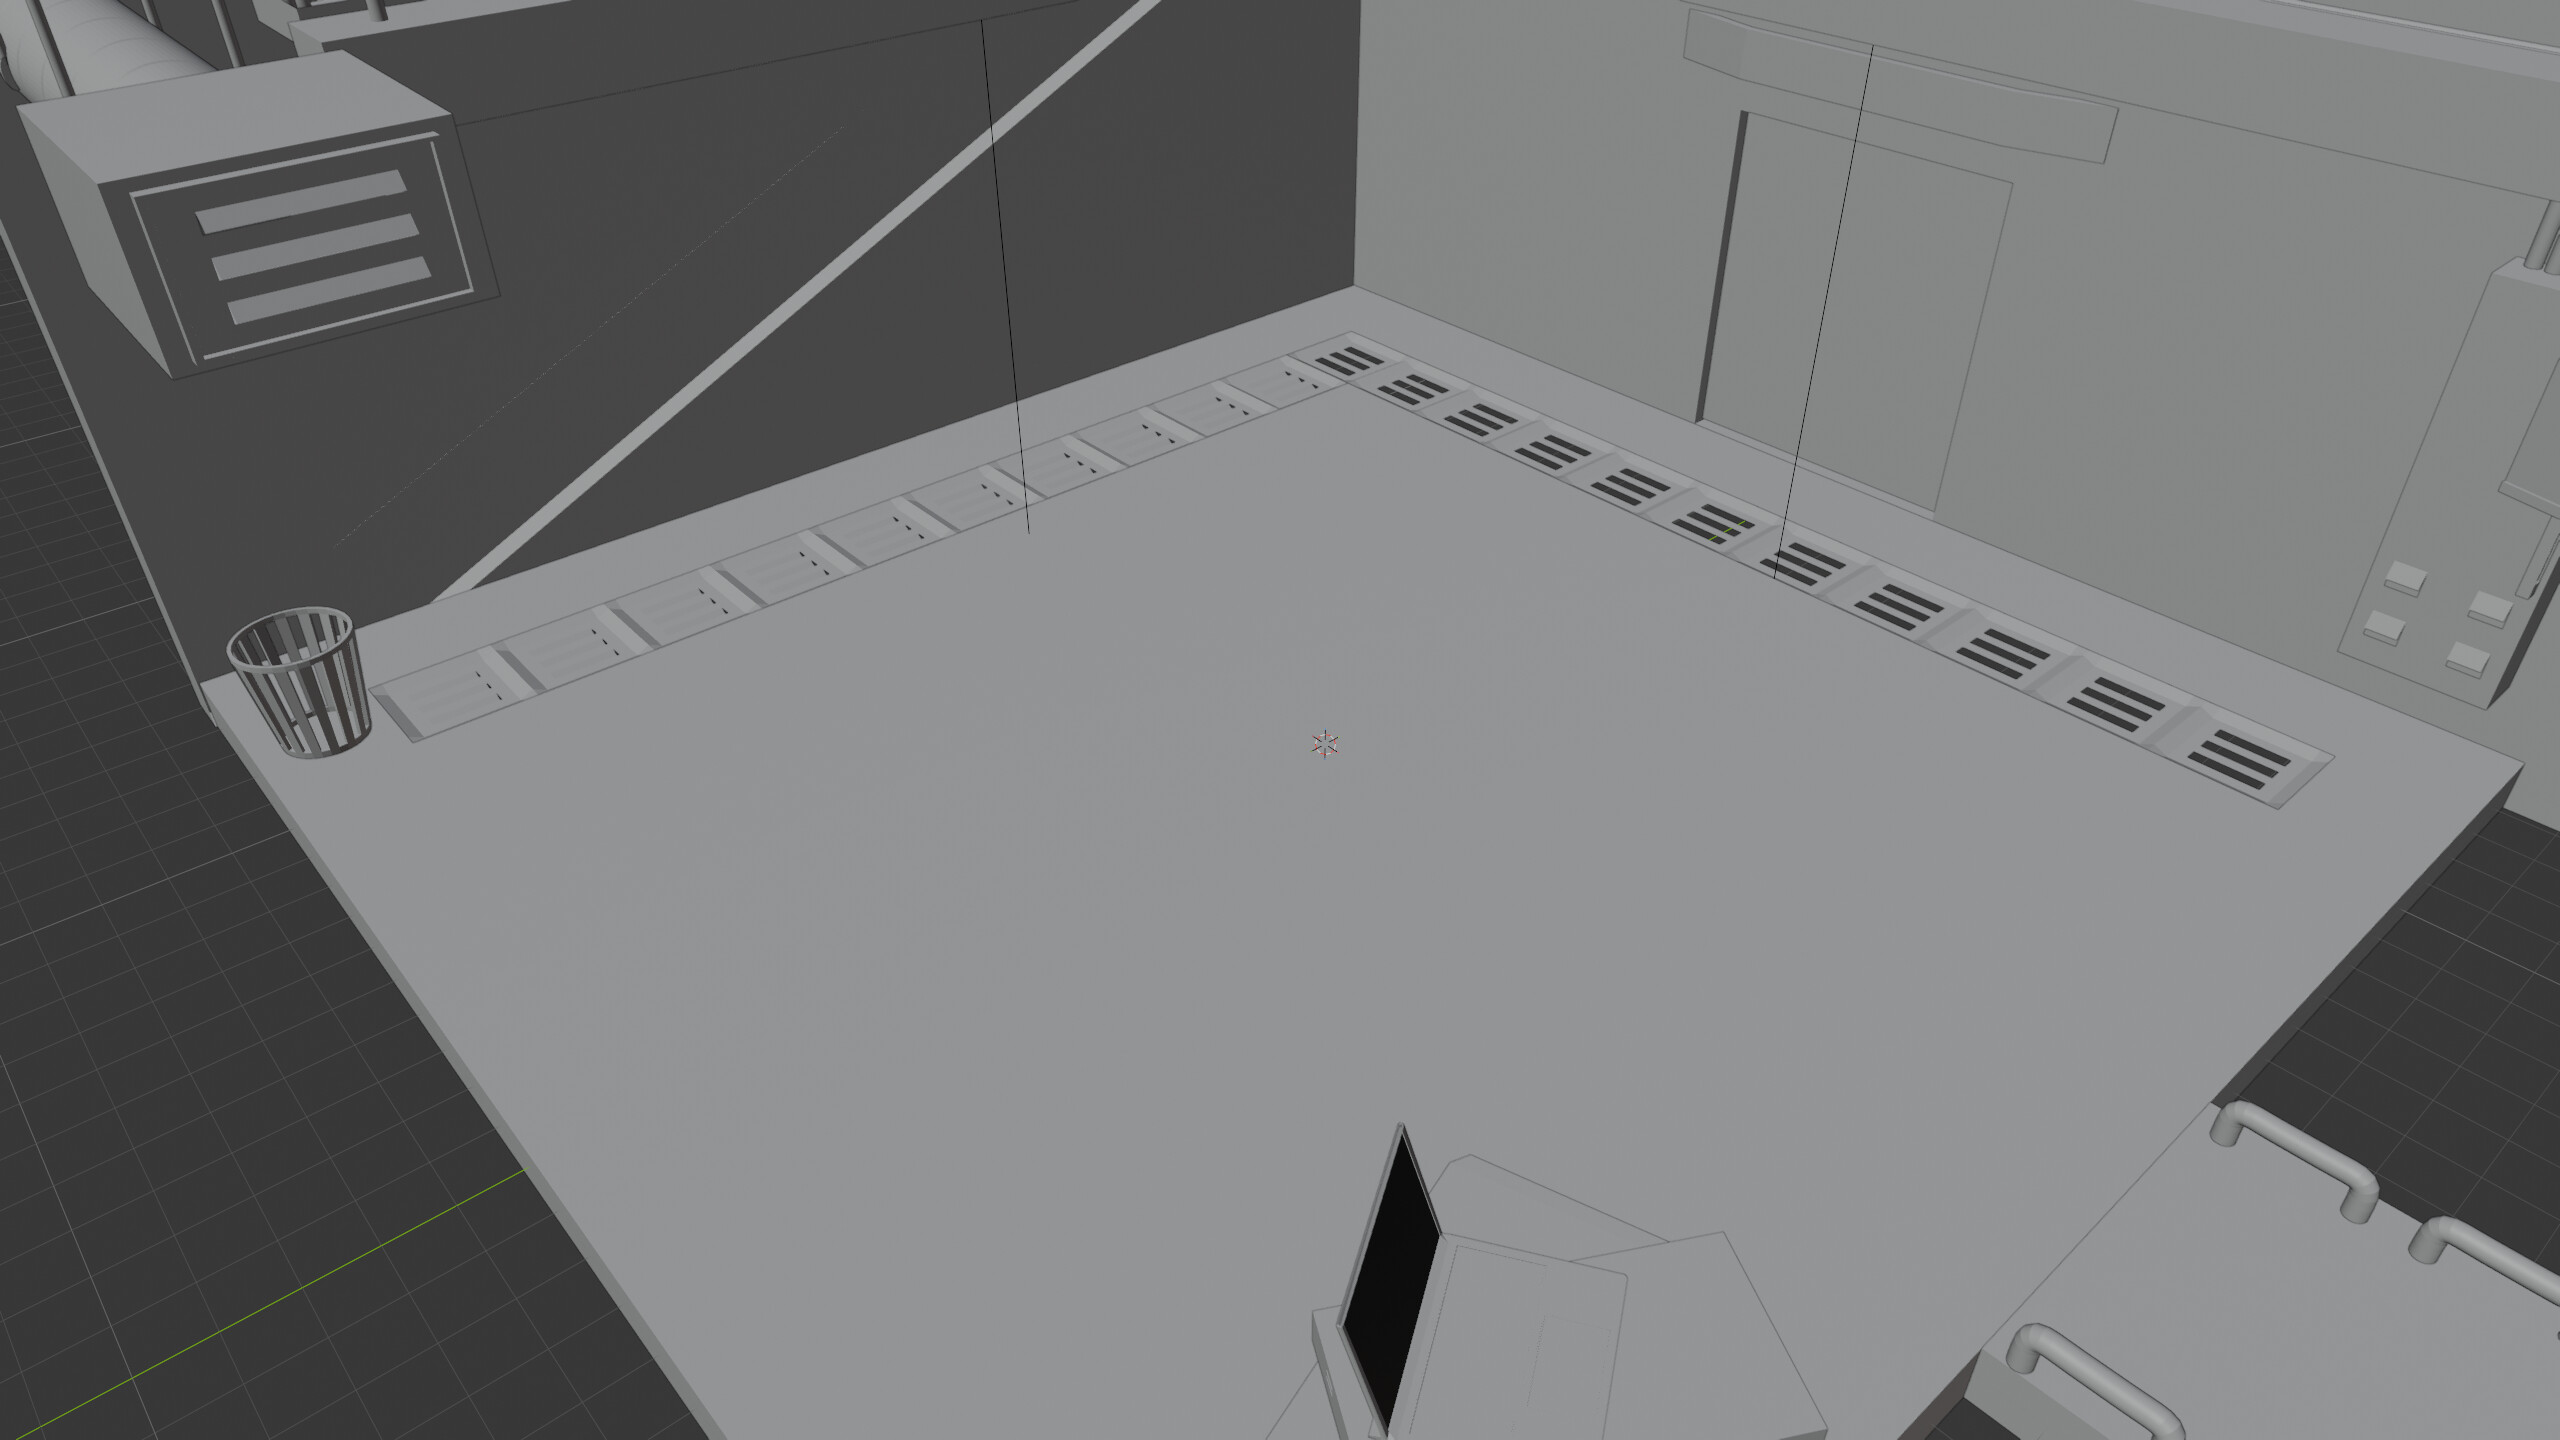
\includegraphics[width=\textwidth]{images/Floor_ViewPort.jpg}
        \caption{Vista de \textit{Viewport} do piso do cenário do jogo.}
        \label{FloorCenarioViewPort}
    \end{minipage}
    \hfill
    \begin{minipage}{0.48\textwidth}
        \centering
        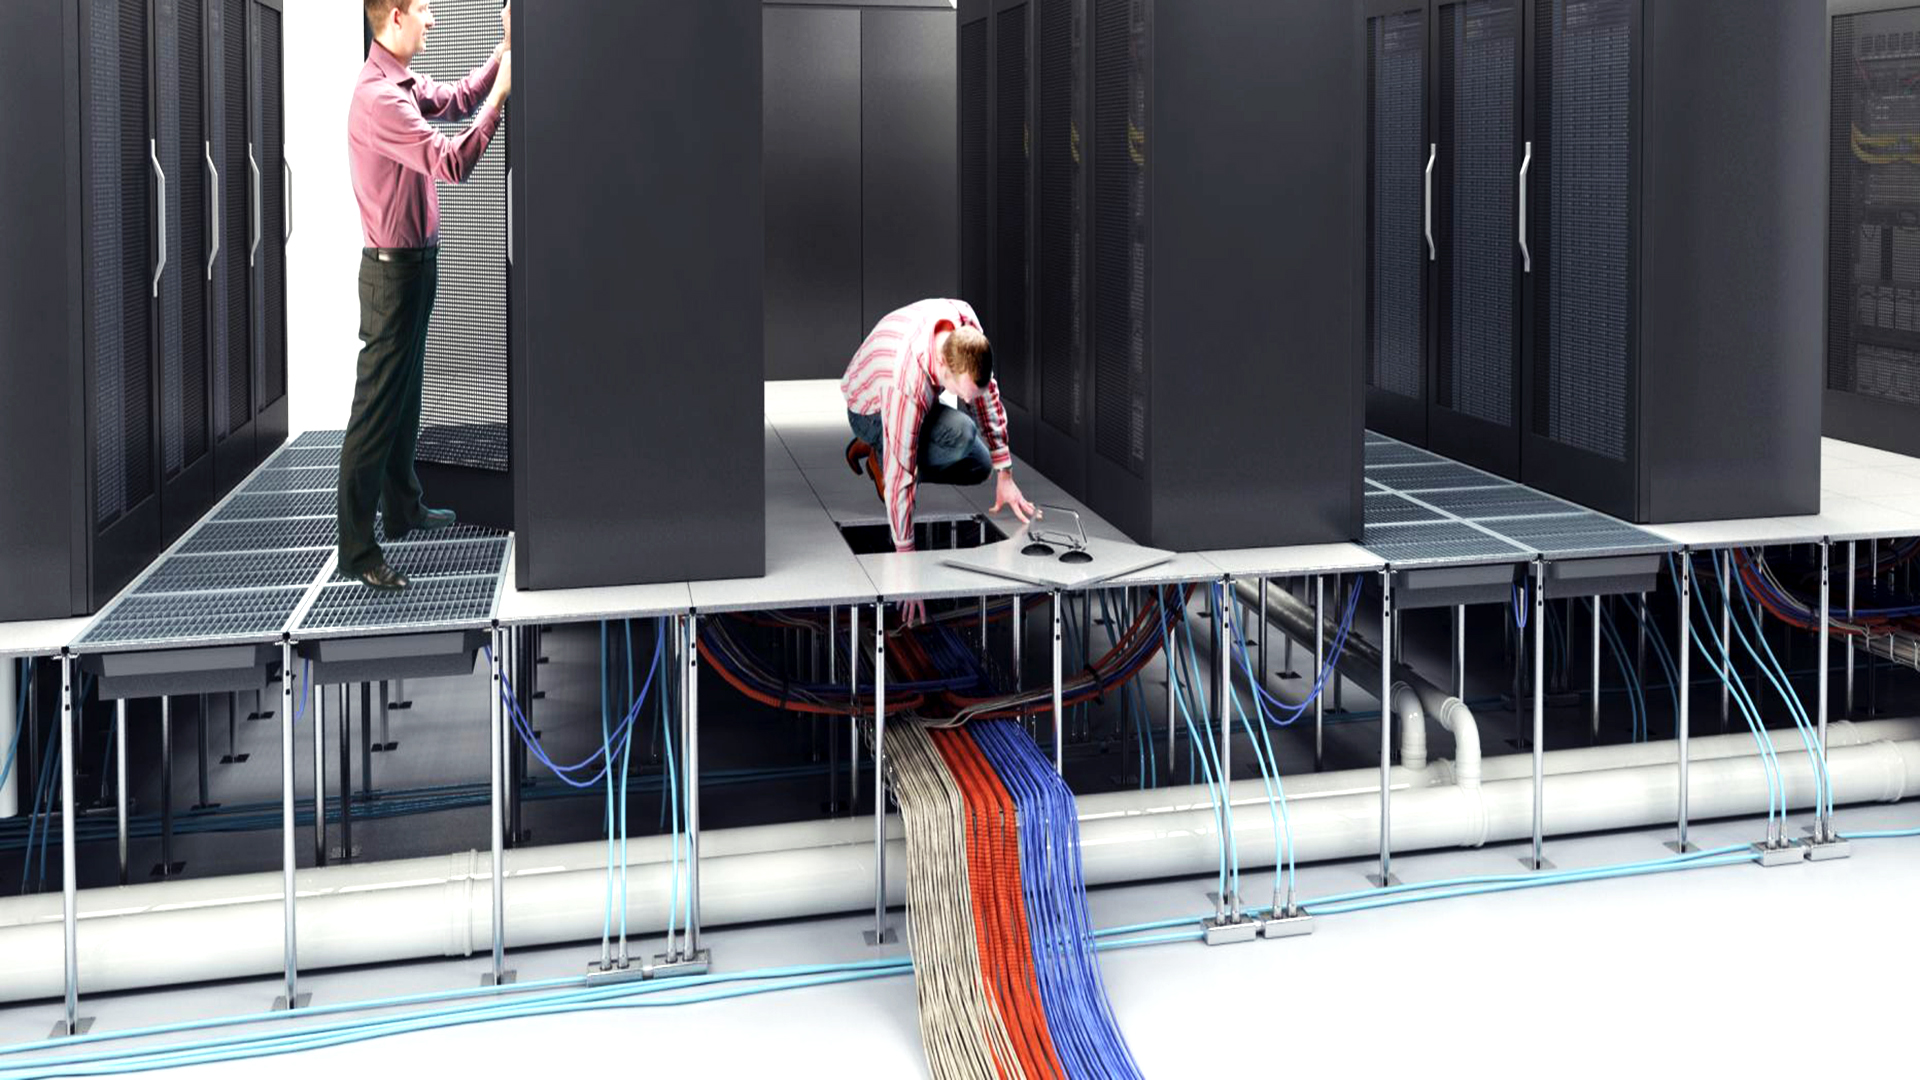
\includegraphics[width=\textwidth]{images/Pavimento Tecnico.jpg}
        \caption{Ilustração do pavimento técnico.}
        \label{PavimentoTecnico}
    \end{minipage}
\end{figure}

Analisando o cenário da Figura \ref{FloorCenarioViewPort} é possível observar a presença de umas caixas no chão, que apresenta algumas perfurações, estas caixas têm como finalidade representar o pavimento técnico ou pavimento elevado, representado na Figura \ref{PavimentoTecnico}, que é um elemento comum em data centers, e tem a função de permitir a passagem de cabos e sistemas de refrigeração, além de facilitar o acesso aos equipamentos instalados no chão do data center.
A representação no jogo é uma adaptação do pavimento técnico real, onde as caixas foram simplificadas, e a fiação de cabos fui desconsiderada. A sua localização no cenário, também serve de marcação para o jogador, uma vez que sempre que existe a compra de um novo servidor, o mesmo é colocado atrás de uma dessas caixas.

\begin{figure}[H]
    \centering
    \begin{minipage}{0.48\textwidth}
        \centering
        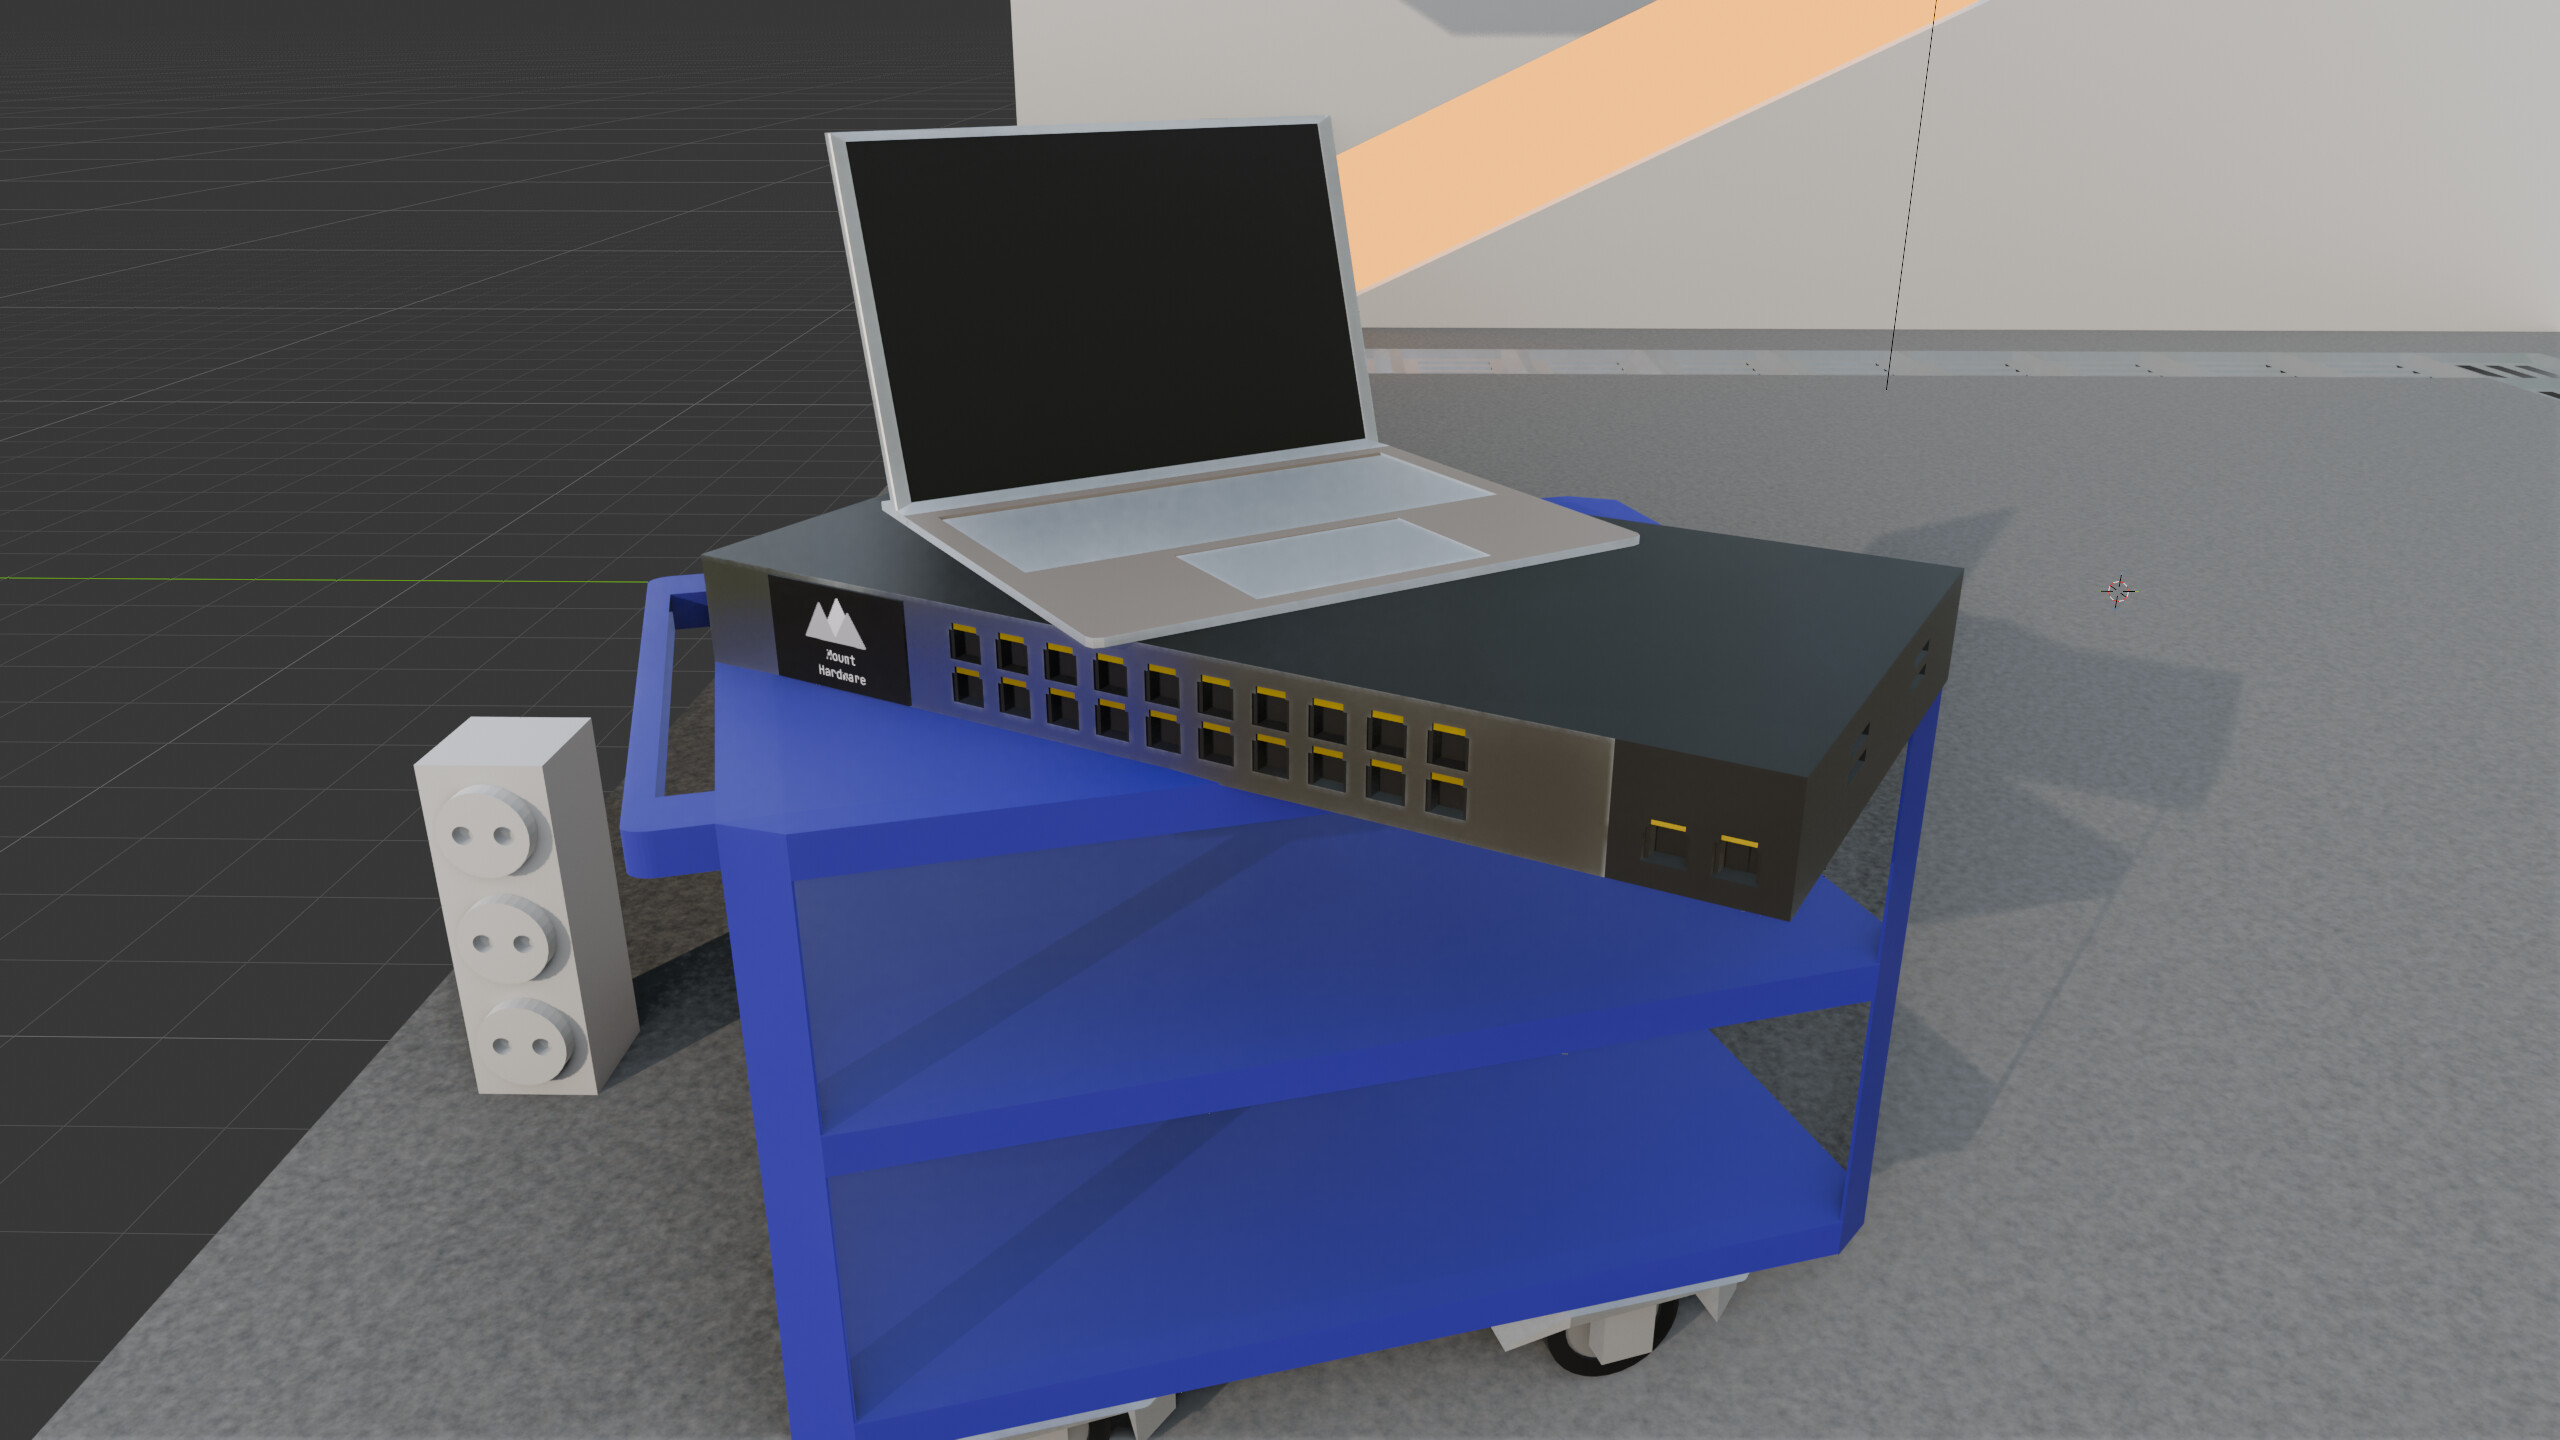
\includegraphics[width=\textwidth]{images/SwitchViewPort.jpg}
        \caption{Vista de \textit{Viewport} do switch de rede.}
        \label{SwitchCenarioViewPort}
    \end{minipage}
    \hfill
    \begin{minipage}{0.48\textwidth}
        \centering
        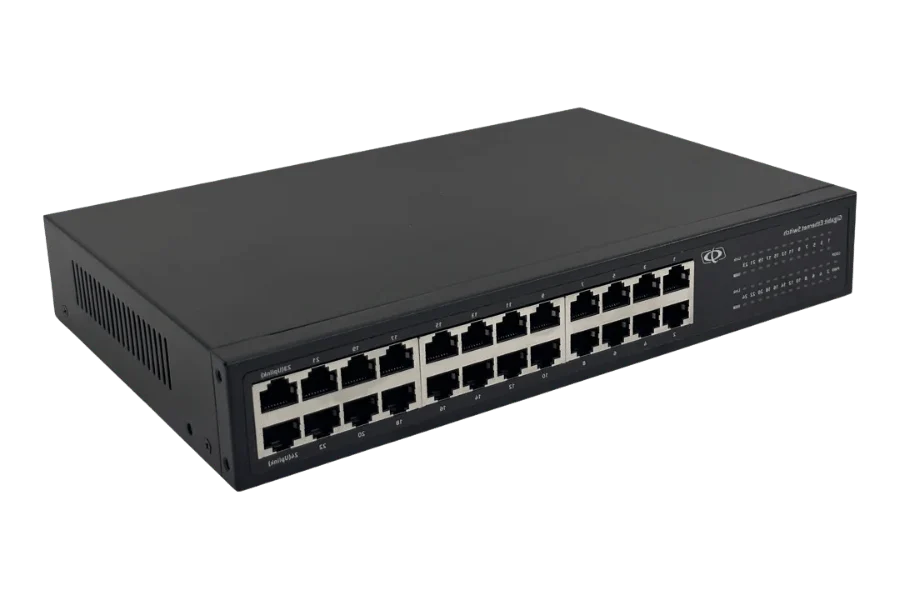
\includegraphics[width=\textwidth]{images/Switch.png}
        \caption{Ilustração do switch de rede.}
        \label{Switch}
    \end{minipage}
\end{figure}

Além da estrutura do próprio cenário, os elementos de decoração presentes nele, são igualmente relevantes para a caracterização do espaço. Assim sendo houve o cuidado de criar elementos que remetem para o contexto de data center, tais como o switch representando na Figura \ref{SwitchCenarioViewPort}. O switch é um equipamento de rede utilizado para conectar vários dispositivos em uma mesma rede local. A representação do switch no jogo é uma adaptação de um switch real, mostrado na figura \ref{Switch}.

\begin{figure}[H]
    \centering
    \begin{minipage}{0.48\textwidth}
        \centering
        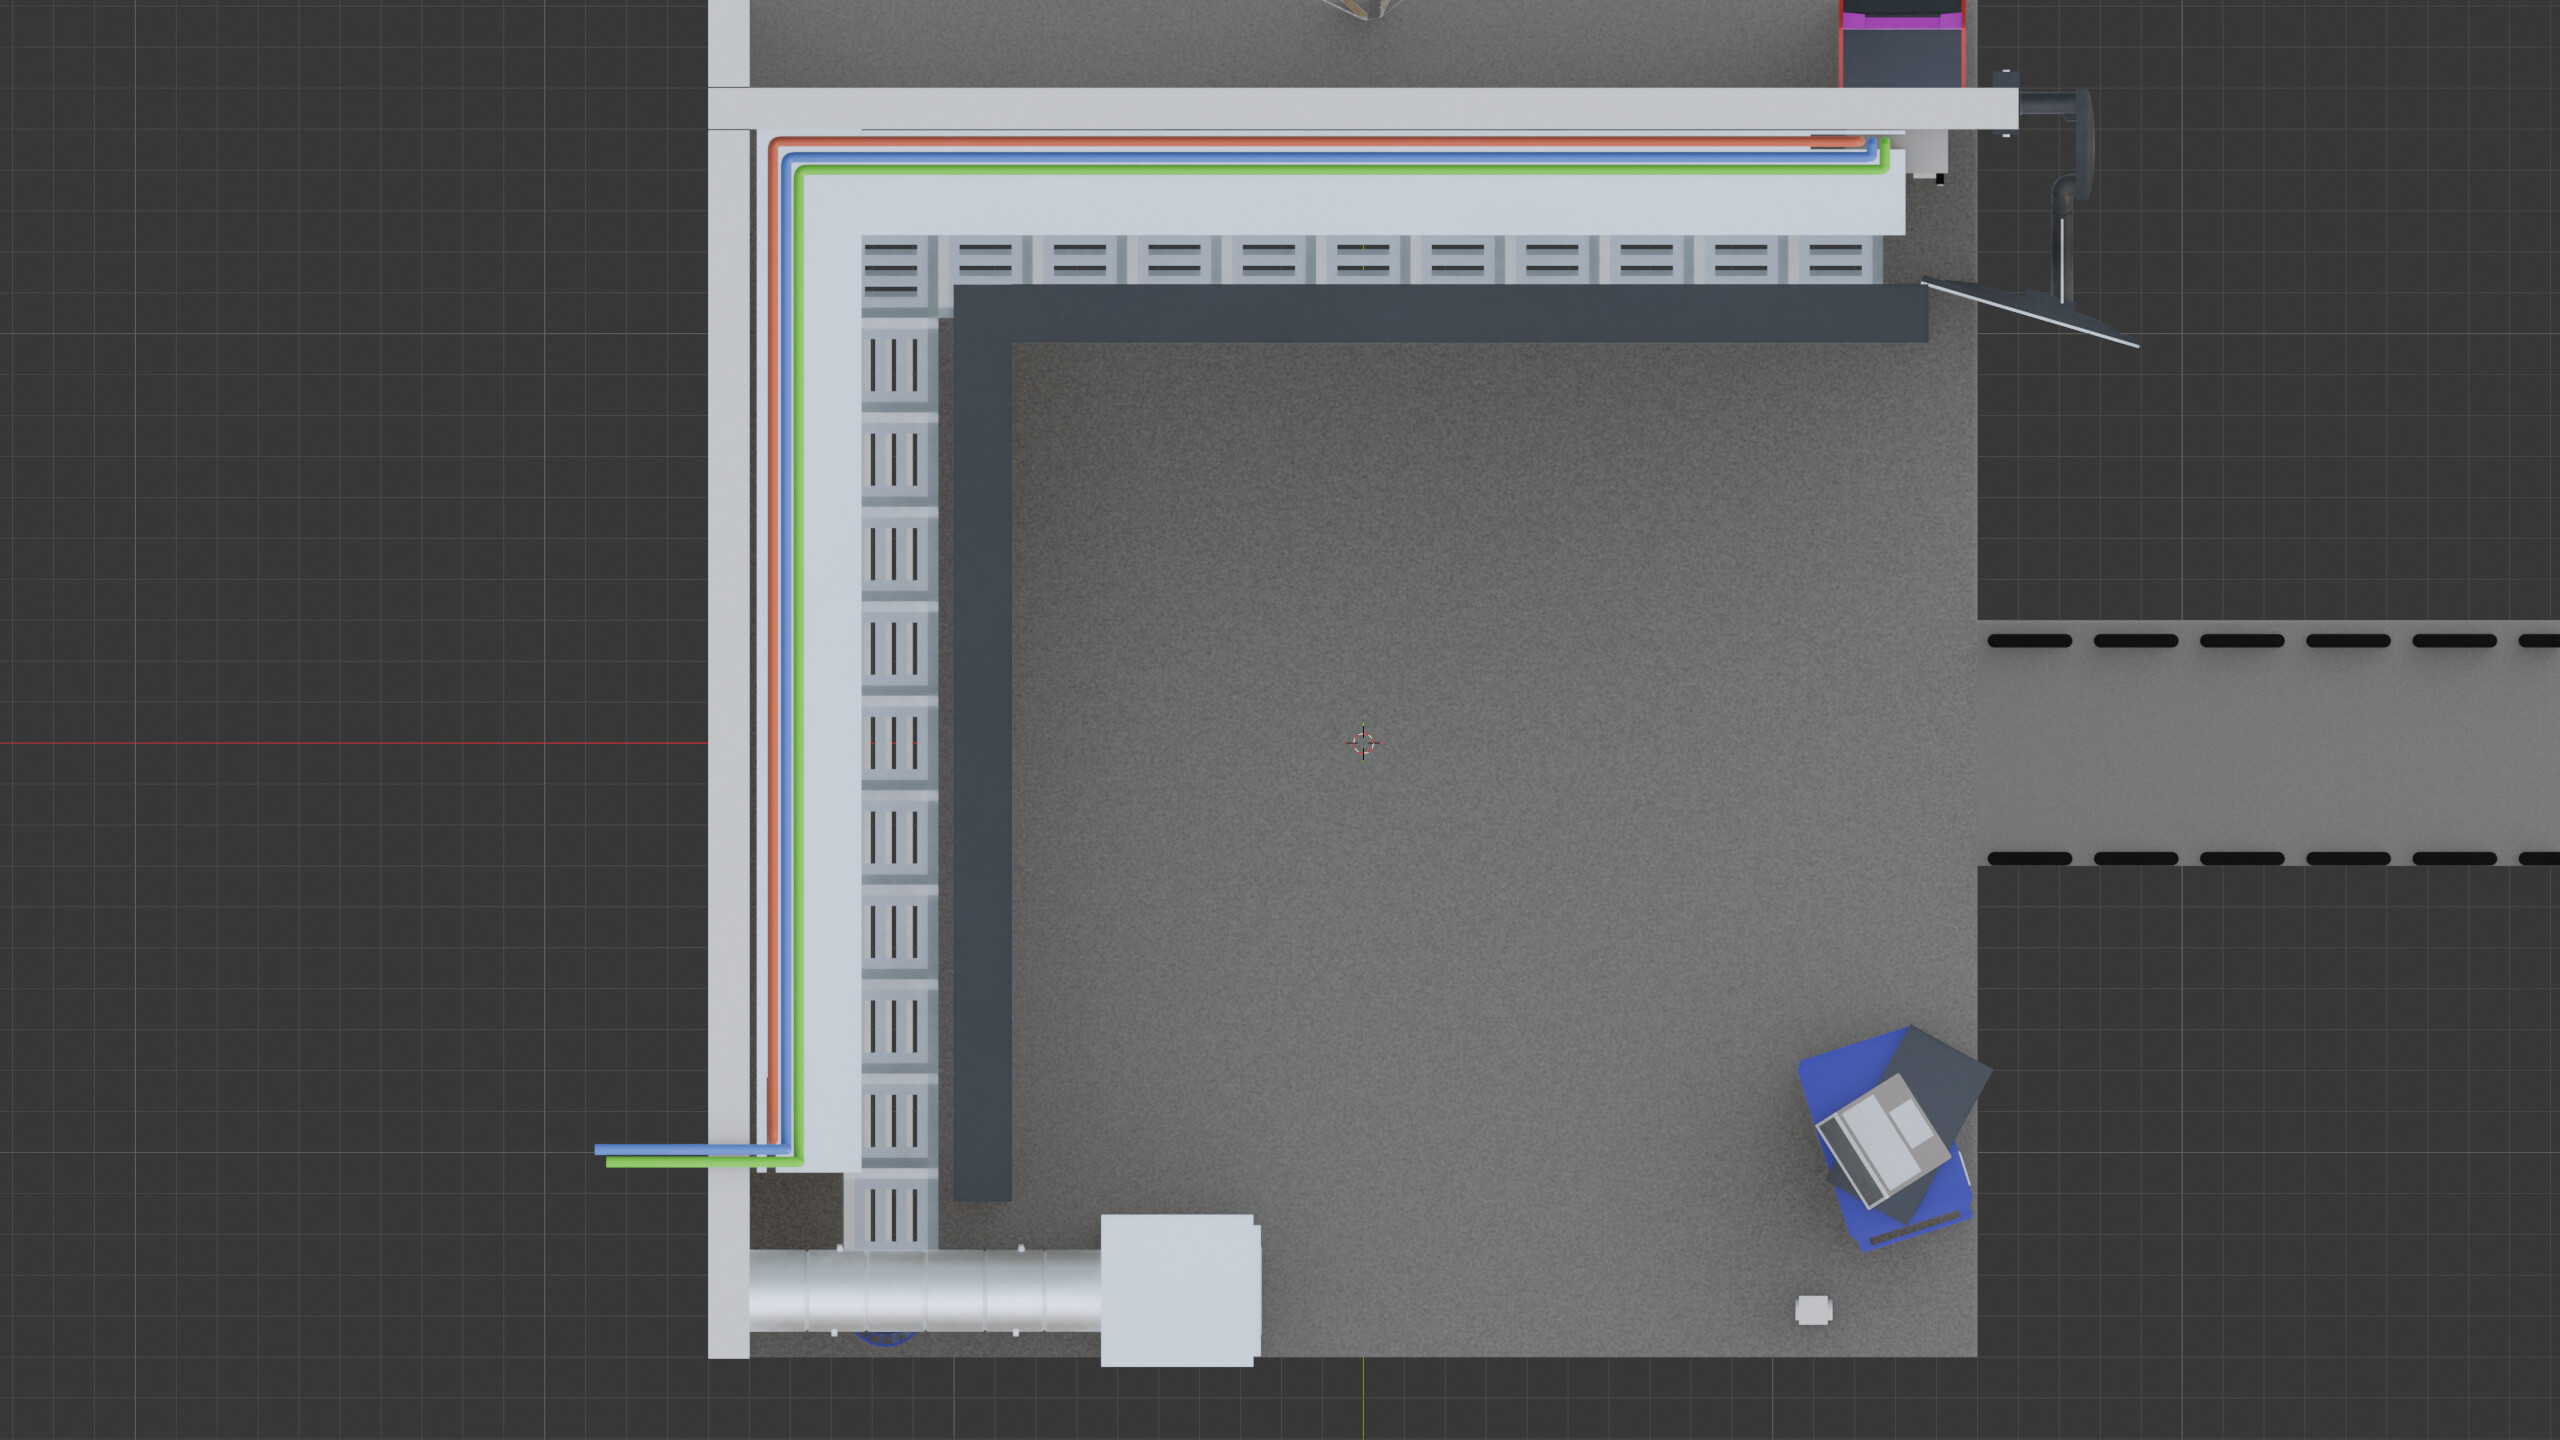
\includegraphics[width=\textwidth]{images/CabesViewPort.jpg}
        \caption{Vista de \textit{Viewport} do caminho de cabos (Vista de cima).}
        \label{CabesCenarioViewPort}
    \end{minipage}
    \hfill
    \begin{minipage}{0.48\textwidth}
        \centering
        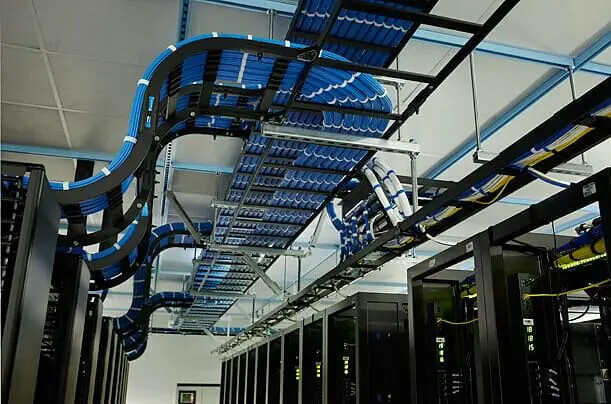
\includegraphics[width=\textwidth]{images/CaminhoCabos.jpg}
        \caption{Ilustração do caminho dos cabos.}
        \label{CaminhoCabos}
    \end{minipage}
\end{figure}

Na parte superior do cenário, existe outro detalhe de decoração, bastante importante para a caracterização do espaço, que é o caminho de cabos, representado na Figura \ref{CabesCenarioViewPort}. Um caminho de cabos, é na sua essência, uma calha colocada geralmente no teto, que tem a função de organizar, proteger e transportar os cabos de rede, energia e outros pelo espaço do data center.
Na Figura \ref{CaminhoCabos} pode ser vista uma representação realista do mesmo.

Na Figura \ref{CabesCenarioViewPort} é possível observar uma representação de um sistema de ventilação e refrigeração, que é um elemento essencial em data centers, uma vez que tem a função de manter a temperatura e a umidade do ambiente controladas, garantindo o bom funcionamento dos equipamentos. A representação do sistema de ventilação e refrigeração no jogo é uma adaptação de um sistema real, onde os detalhes foram simplificados para se adequar ao estilo visual do jogo.

\begin{figure}[H]
    \centering
    \begin{minipage}{0.48\textwidth}
        \centering
        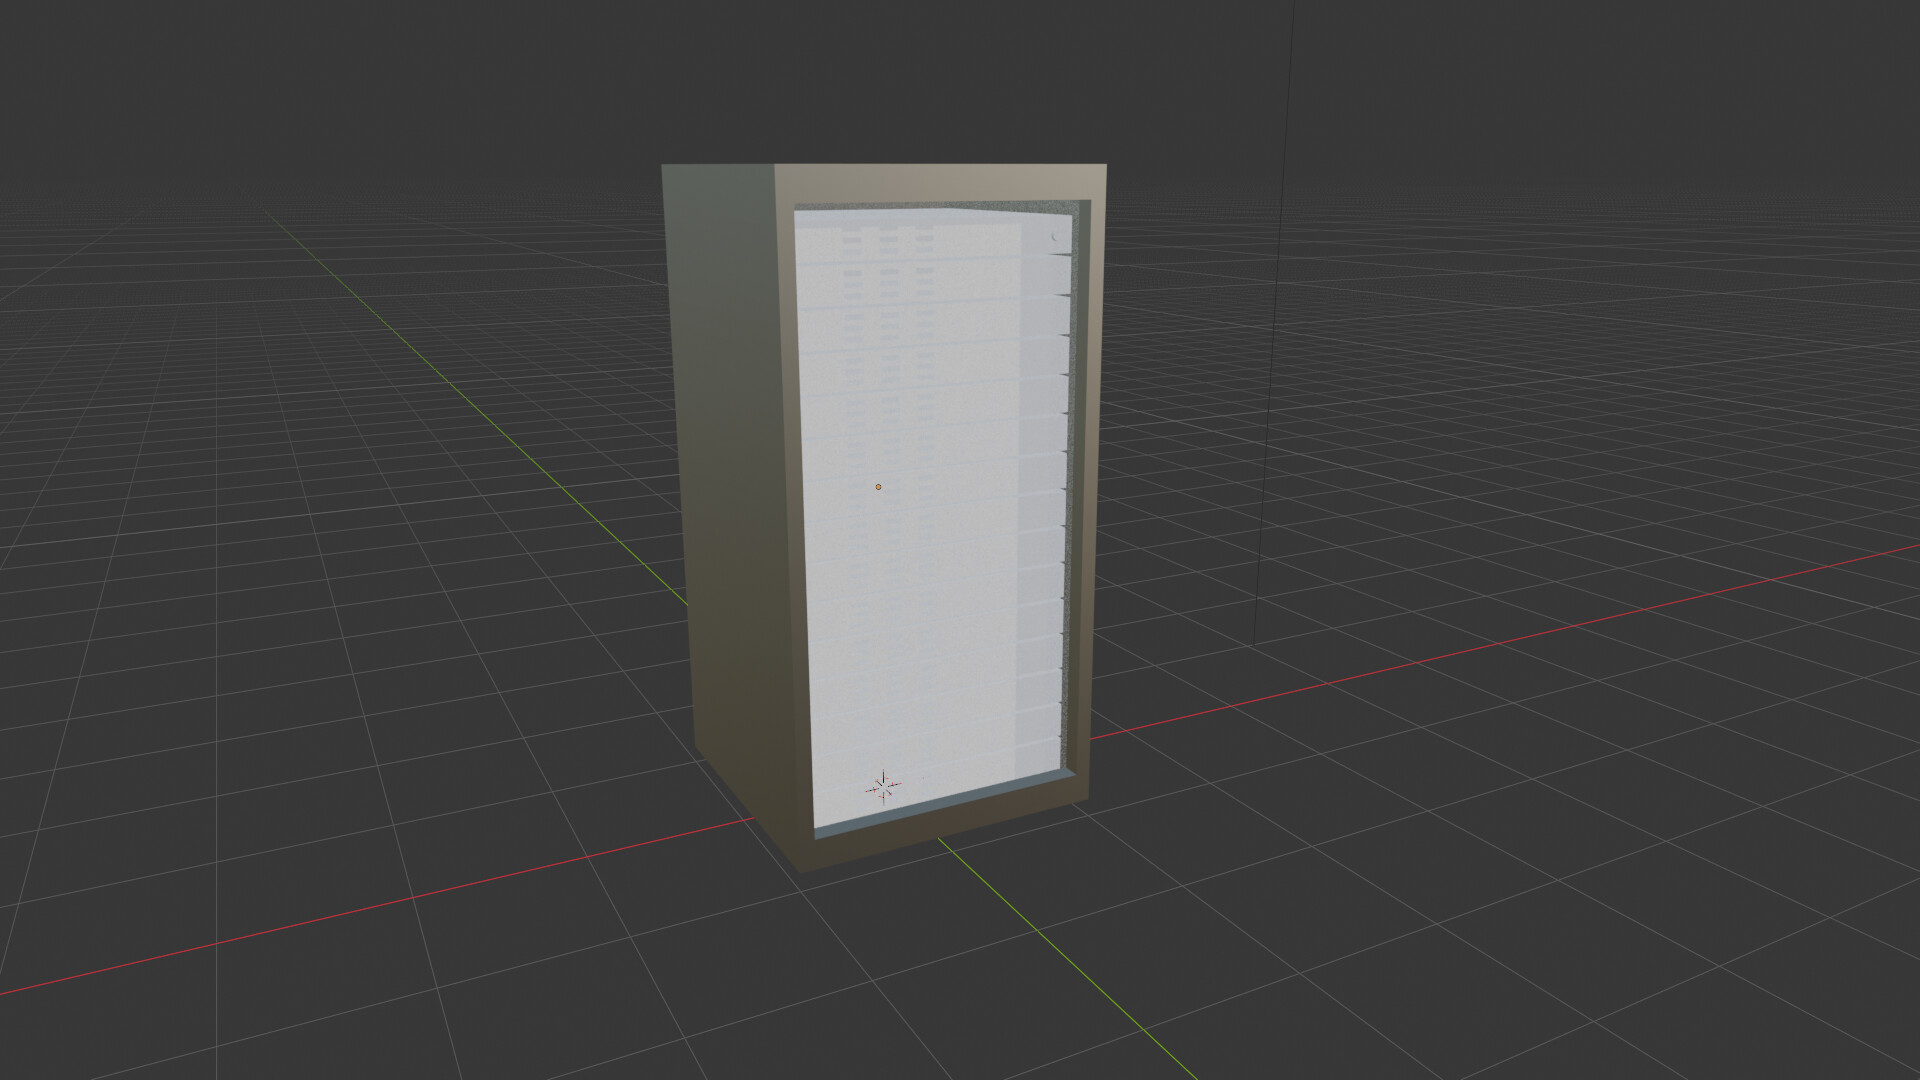
\includegraphics[width=\textwidth]{images/ServidorViewPort.jpg}
        \caption{Vista de \textit{Viewport} do servidor.}
        \label{ServidorViewPort}
    \end{minipage}
    \hfill
    \begin{minipage}{0.48\textwidth}
        \centering
        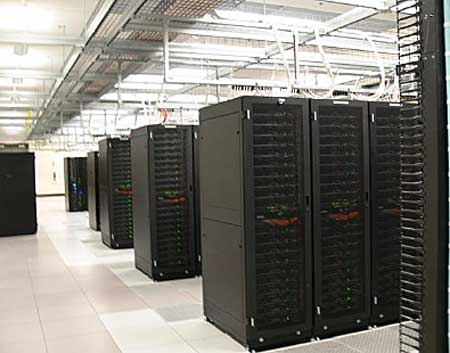
\includegraphics[width=\textwidth]{images/Servidor_Amazon.jpg}
        \caption{Representação do servidor da Amazon.}
        \label{ServidorAmazon}
    \end{minipage}
\end{figure}

A representação de servidores no jogo, assim como se pode ver na Figura \ref{ServidorViewPort}, é uma adaptação de \textit{racks} de servidores reais, conforme é mostrado na Figura \ref{ServidorAmazon}. Os \textit{racks} de servidores são estruturas metálicas que abrigam os equipamentos de um data center, como servidores, switches, roteadores, etc... A representação de servidores no jogo, foi simplificada, no sentido de homogeneizar a aparência de todos os equipamentos e função os limitando apenas servidores, no sentido de computadores.

\begin{figure}[H]
    \centering
    \begin{minipage}{0.48\textwidth}
        \centering
        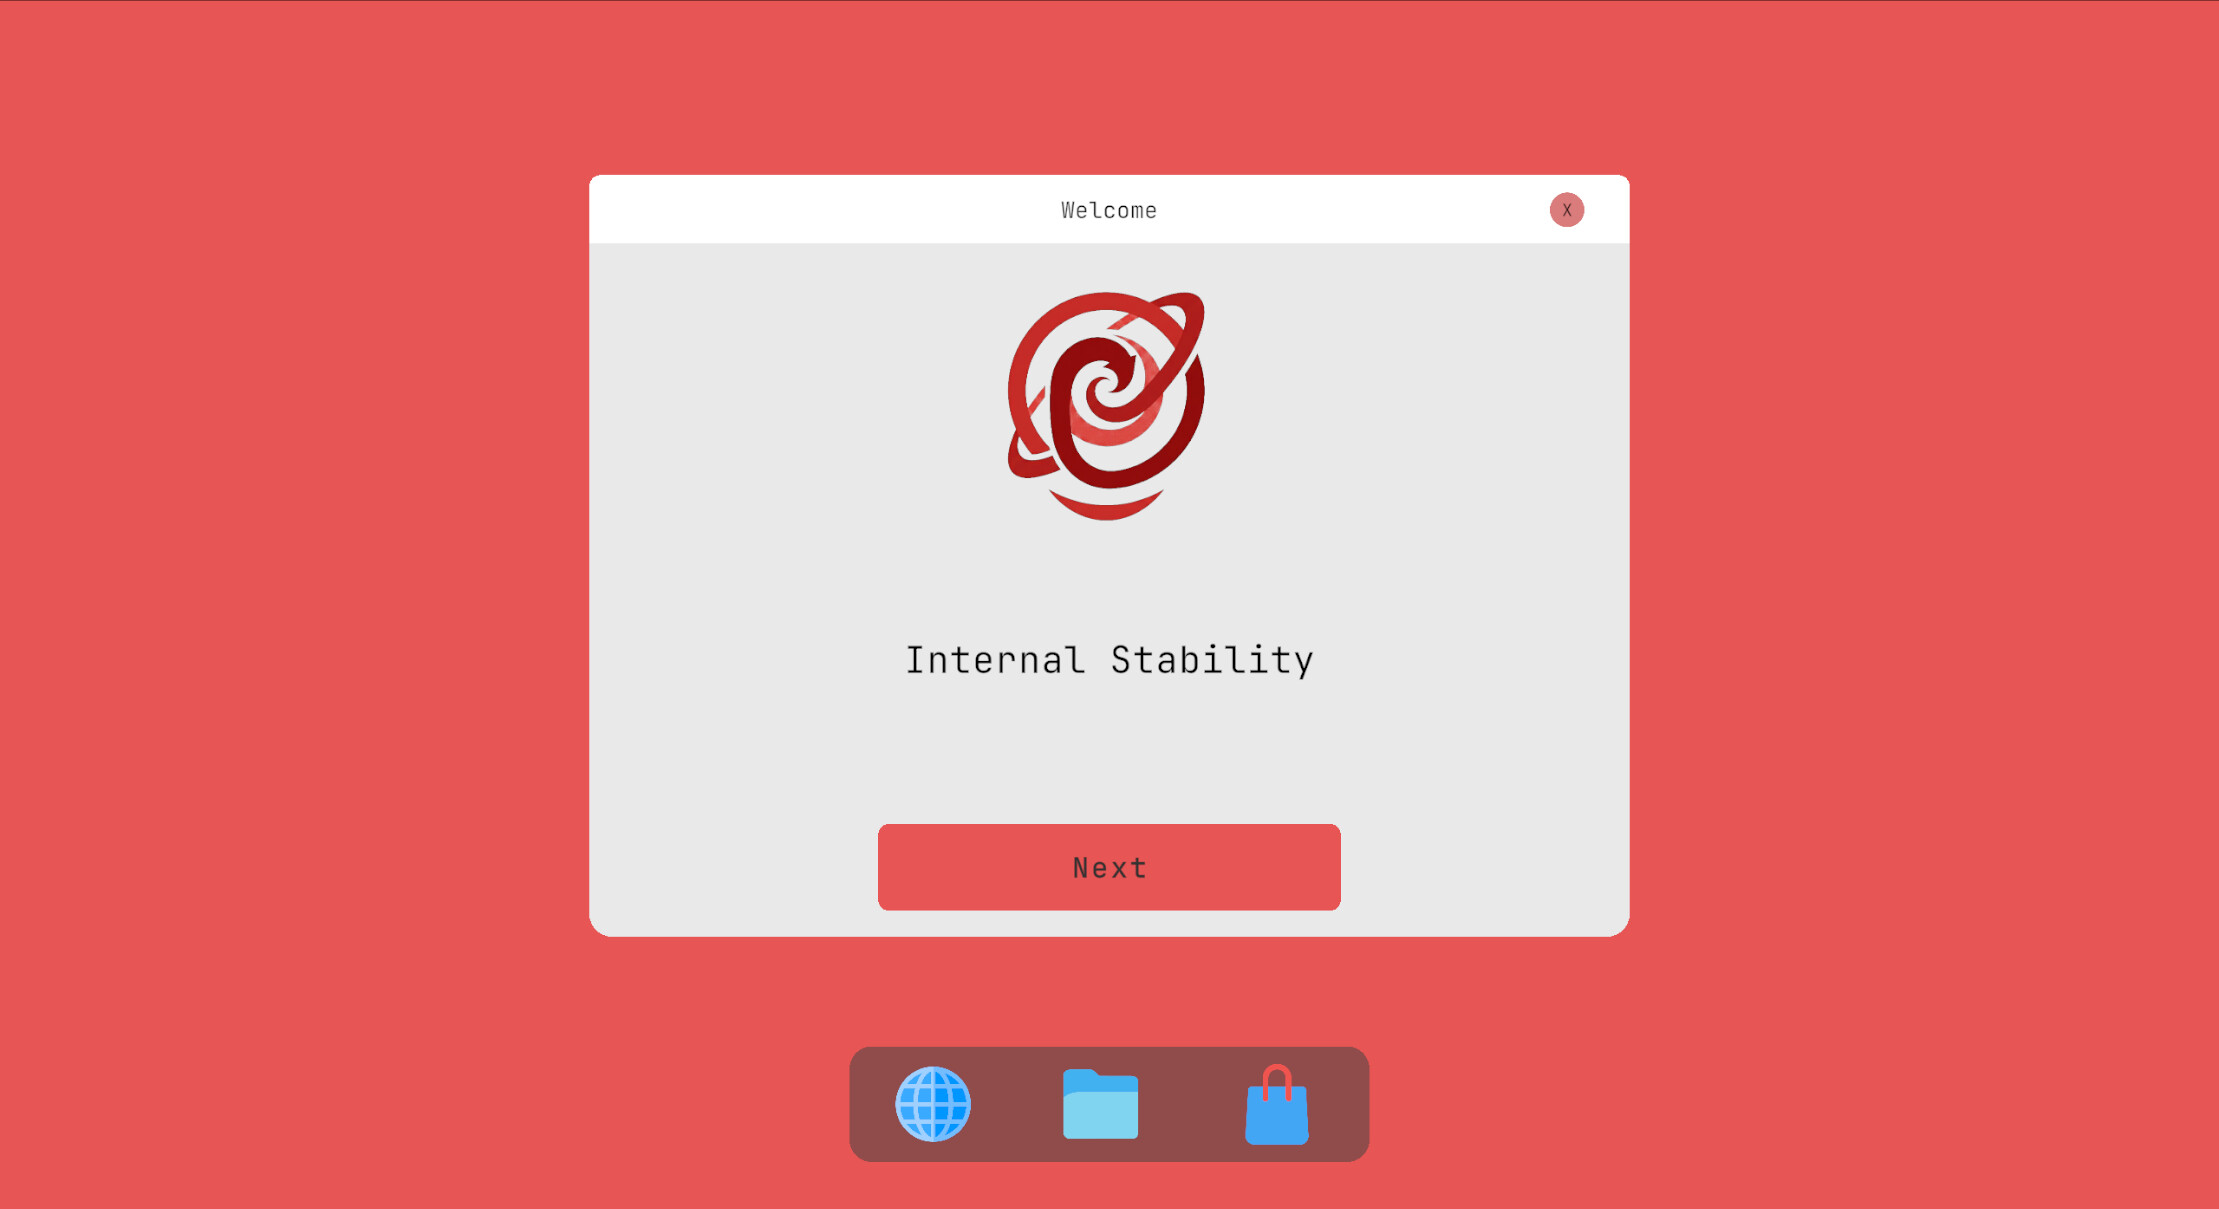
\includegraphics[width=\textwidth]{images/GnomeGame.jpg}
        \caption{\textit{UI} da instalação e configuração de um sistema operativo.}
        \label{GameGnomeUI}
    \end{minipage}
    \hfill
    \begin{minipage}{0.48\textwidth}
        \centering
        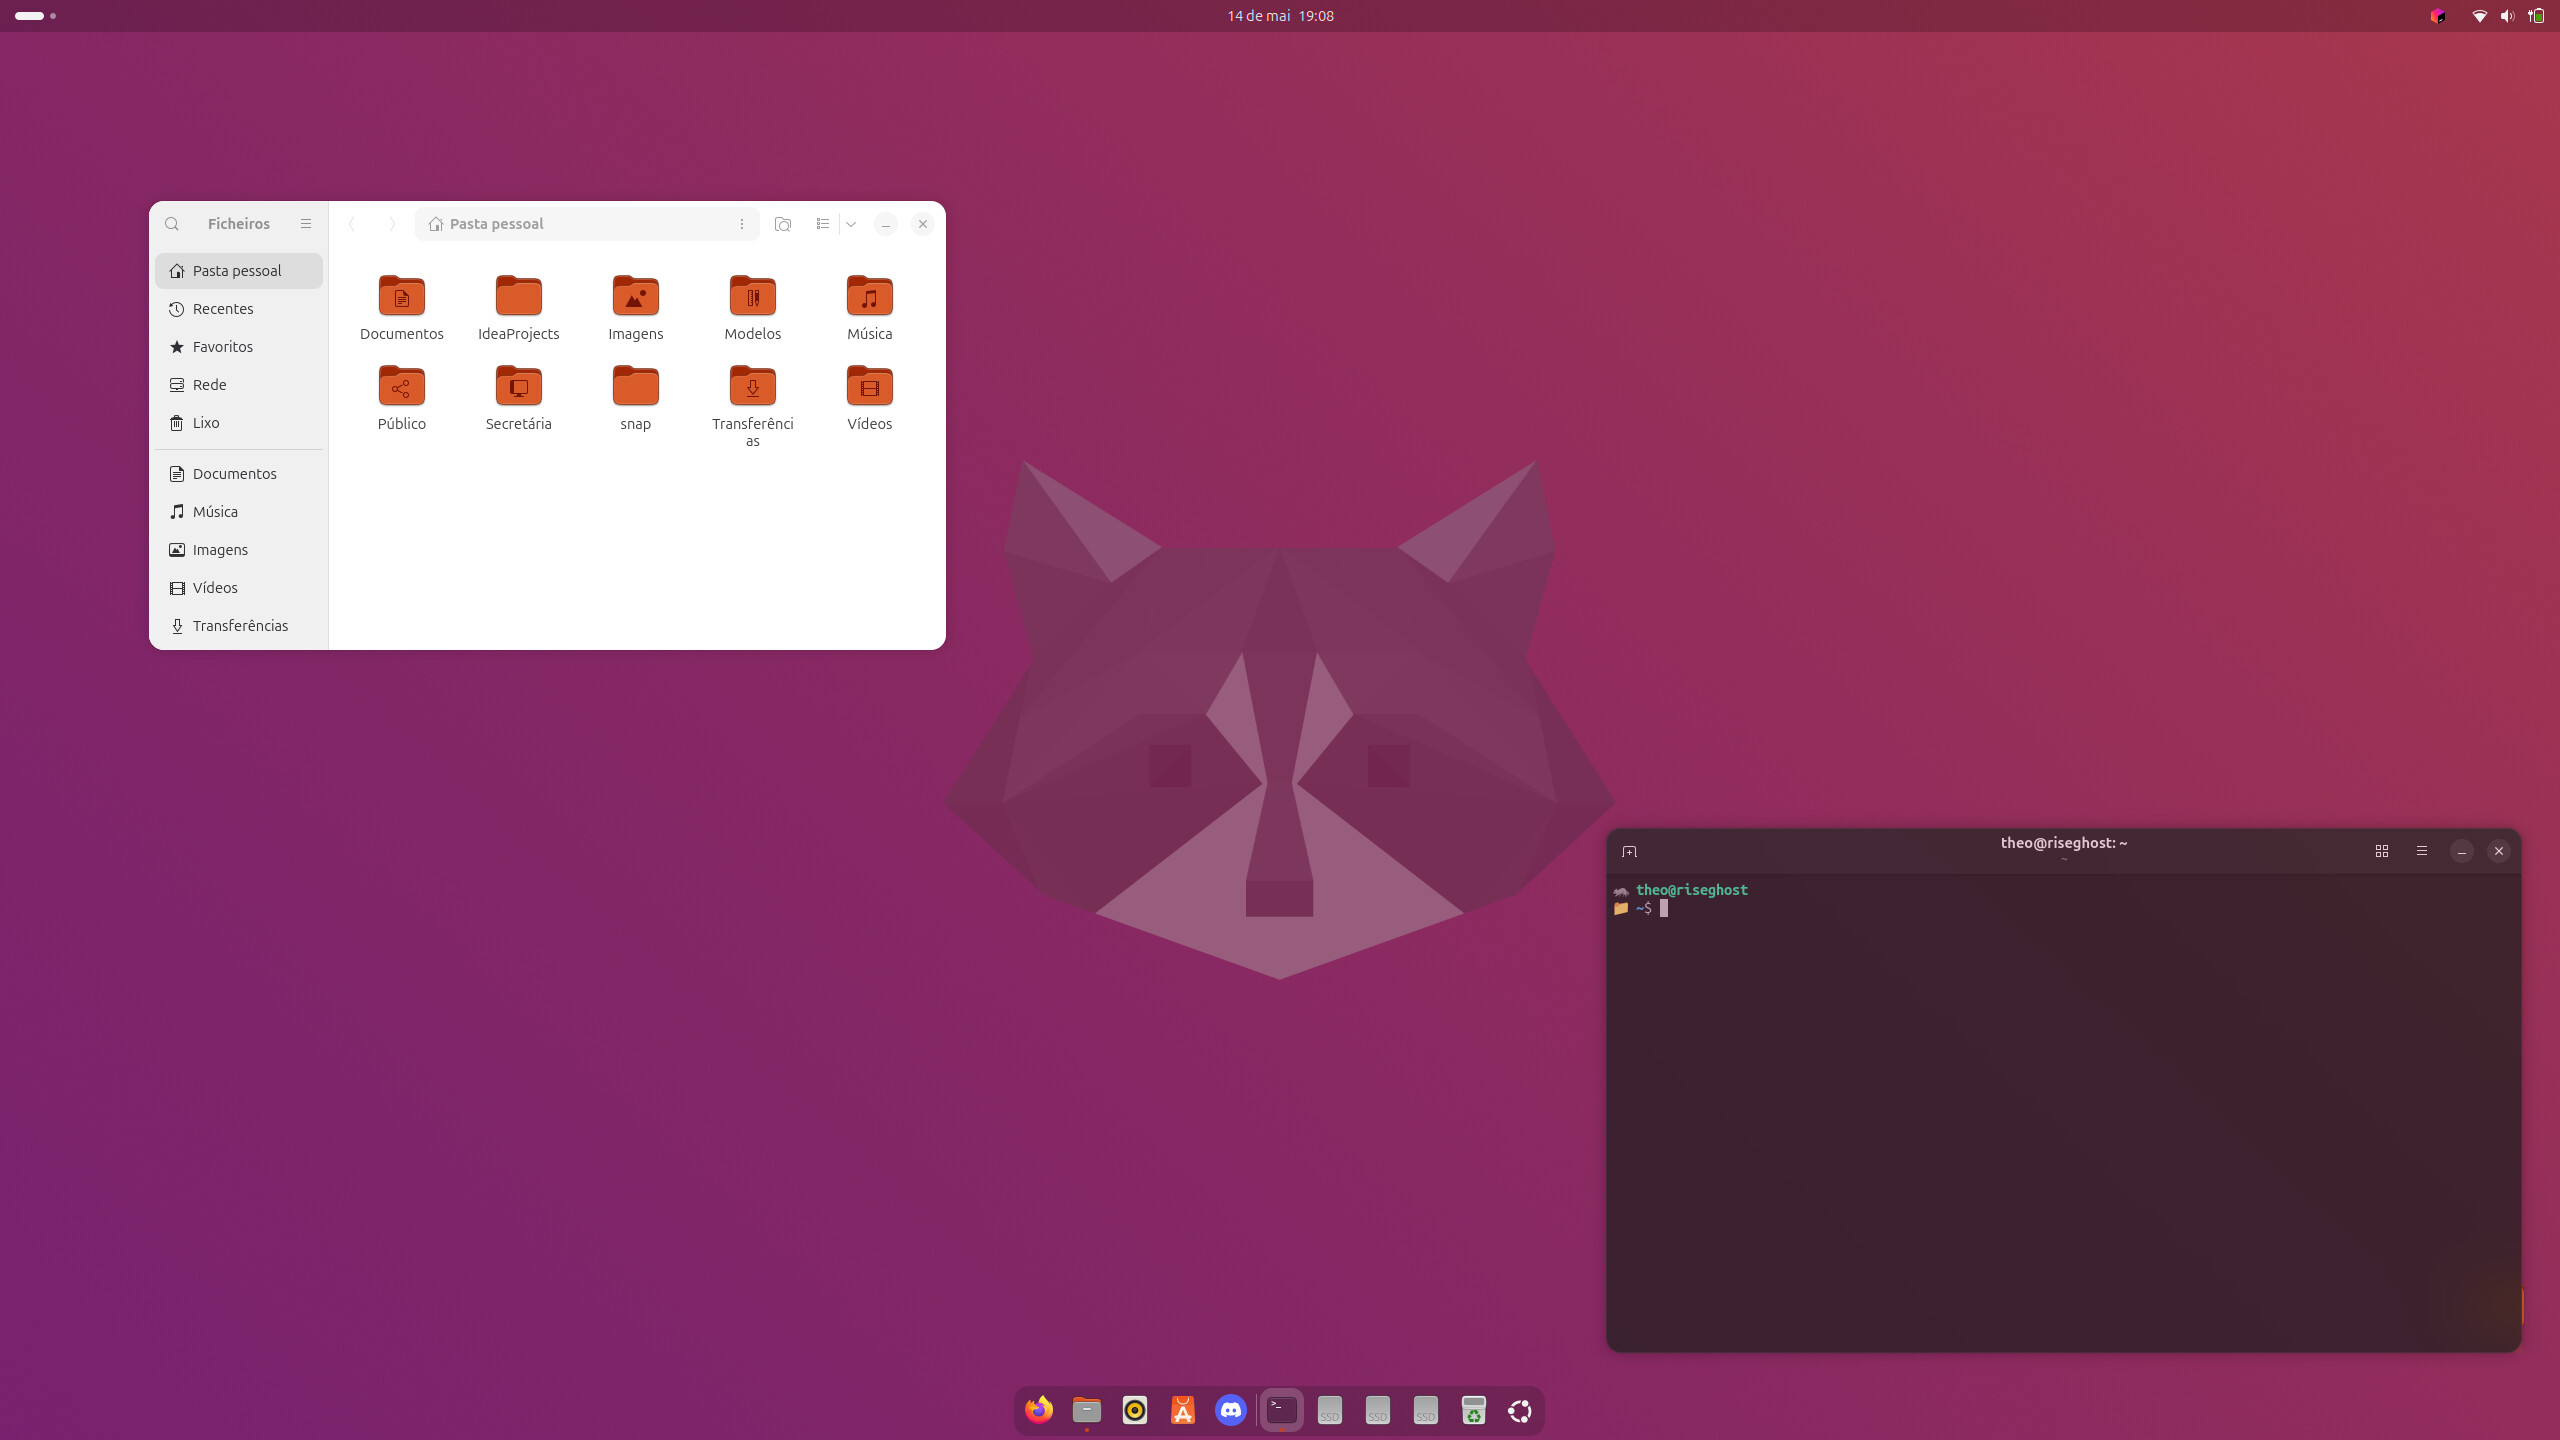
\includegraphics[width=\textwidth]{images/Imagem colada.jpg}
        \caption{Ambiente gráfico Gnome.}
        \label{GnomeUI}
    \end{minipage}
\end{figure}

Por fim, além de elementos gráficos de cenário, elementos de \textit{UI}, tais como a interface de configuração de um sistema operativo, foram igualmente inspirados em referência reais.
Na Figura \ref{GnomeUI} é mostrado a interface gráfica Gnome, que é um ambiente gráfico vastamente utilizado em sistemas operativos Linux, embora a sua utilização em data centers não seja tão comum, ainda assim, é bastante dissolvida no ambiente de tecnologia.
Devia a ser uma interface gráfica mais amigável e intuitiva, servi como inspiração para a construção da interface vista na Figura \ref{GameGnomeUI}.

\section{Desenvolvimento do conceito de jogo}

Este projeto consiste na construção de um vídeo jogo, onde o jogador é responsável
por fazer a gestão de um pequeno data center, onde o objetivo é ganhar dinheiro.

No entanto, durante todo o percurso de \textit{gameplay}, o jogador terá várias etapas a cumprir,
como, comprar equipamento, configurar o equipamento, resolução de pequenos
puzzles disponibilizados sobre a forma de \textit{mini games}, gestão de recursos económicos e 
combate contra ameaças, como, por exemplo, vírus e ataques de \textit{hackers}.

Nas subseções seguintes, será desenvolvido de forma mais detalhada cada um dos pontos
principais do conceito do jogo.

\subsection{Compra e configuração de equipamento}

Durante a compra de equipamentos para o data center, o jogador tem a sua disposição uma interface completa de
configuração, onde é possivel escolher componentes como:
\begin{itemize}
    \item Processadores;
    \item RAM;
    \item Discos de vários tipos;
    \item Placas de rede;
    \item Sistema Operativo;
    \item Sistemas de refrigeração (Está presente de forma simplificada).
\end{itemize}

\begin{figure}[H]
  \centering
  % --- Primeira Figura (Métricas) ---
  \begin{minipage}[b]{0.48\textwidth}
    \centering
    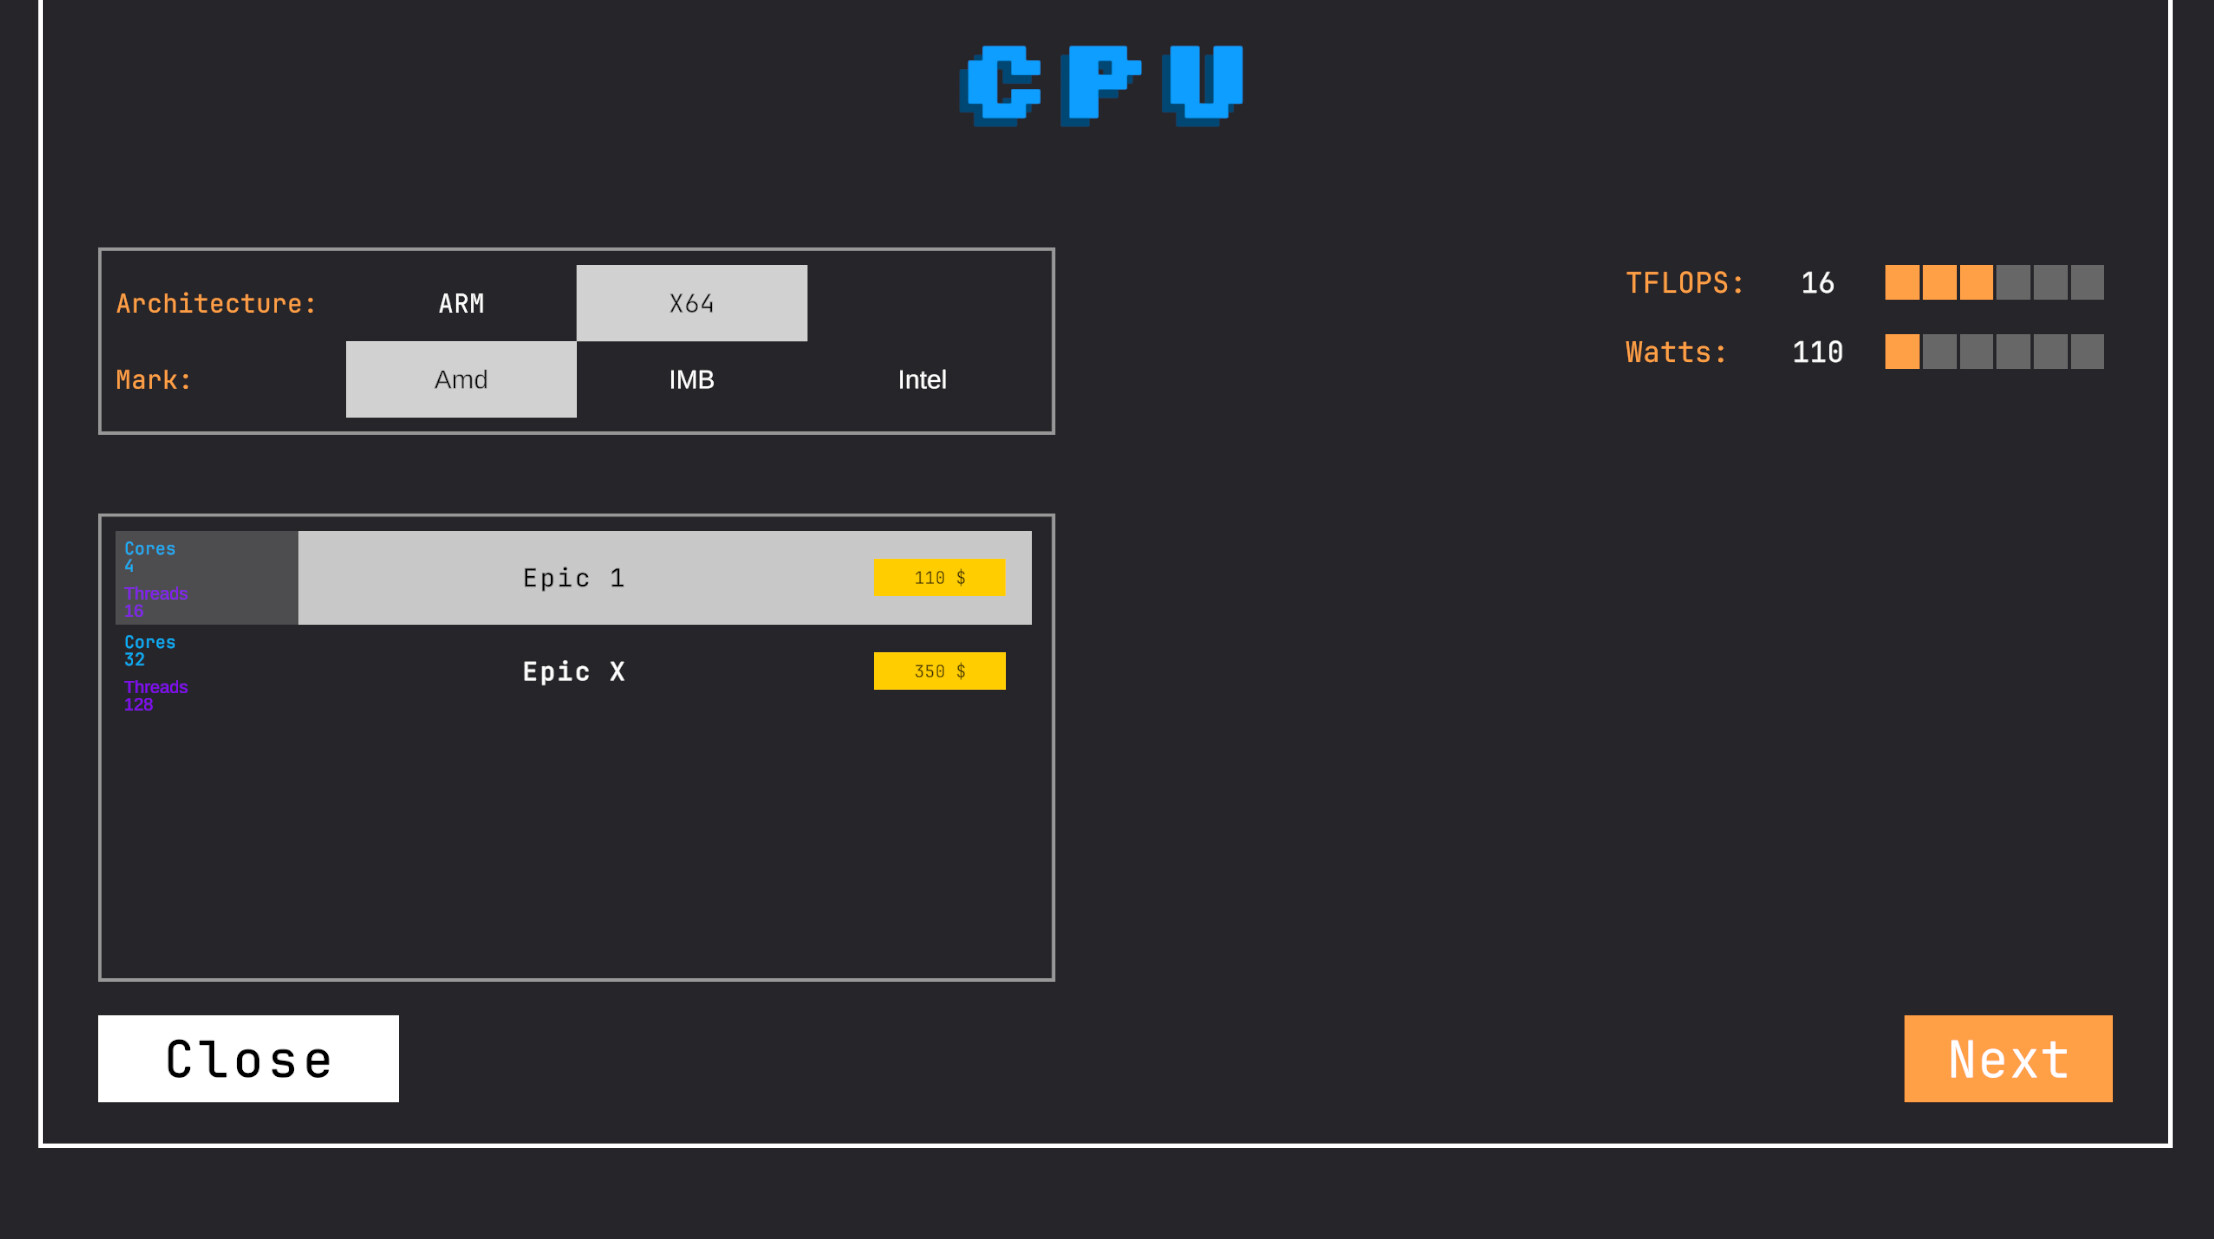
\includegraphics[width=\textwidth]{images/Projeto CPU.jpg}
    \caption[Captura de tela do jogo - Configuração de CPU.]{Captura de tela do jogo - Configuração de CPU.}
    \label{Projeto_config_cpu1}
  \end{minipage}
  \hfill % Espaçamento entre as minipages
  % --- Segunda Figura (Servidores) ---
  \begin{minipage}[b]{0.48\textwidth}
    \centering
    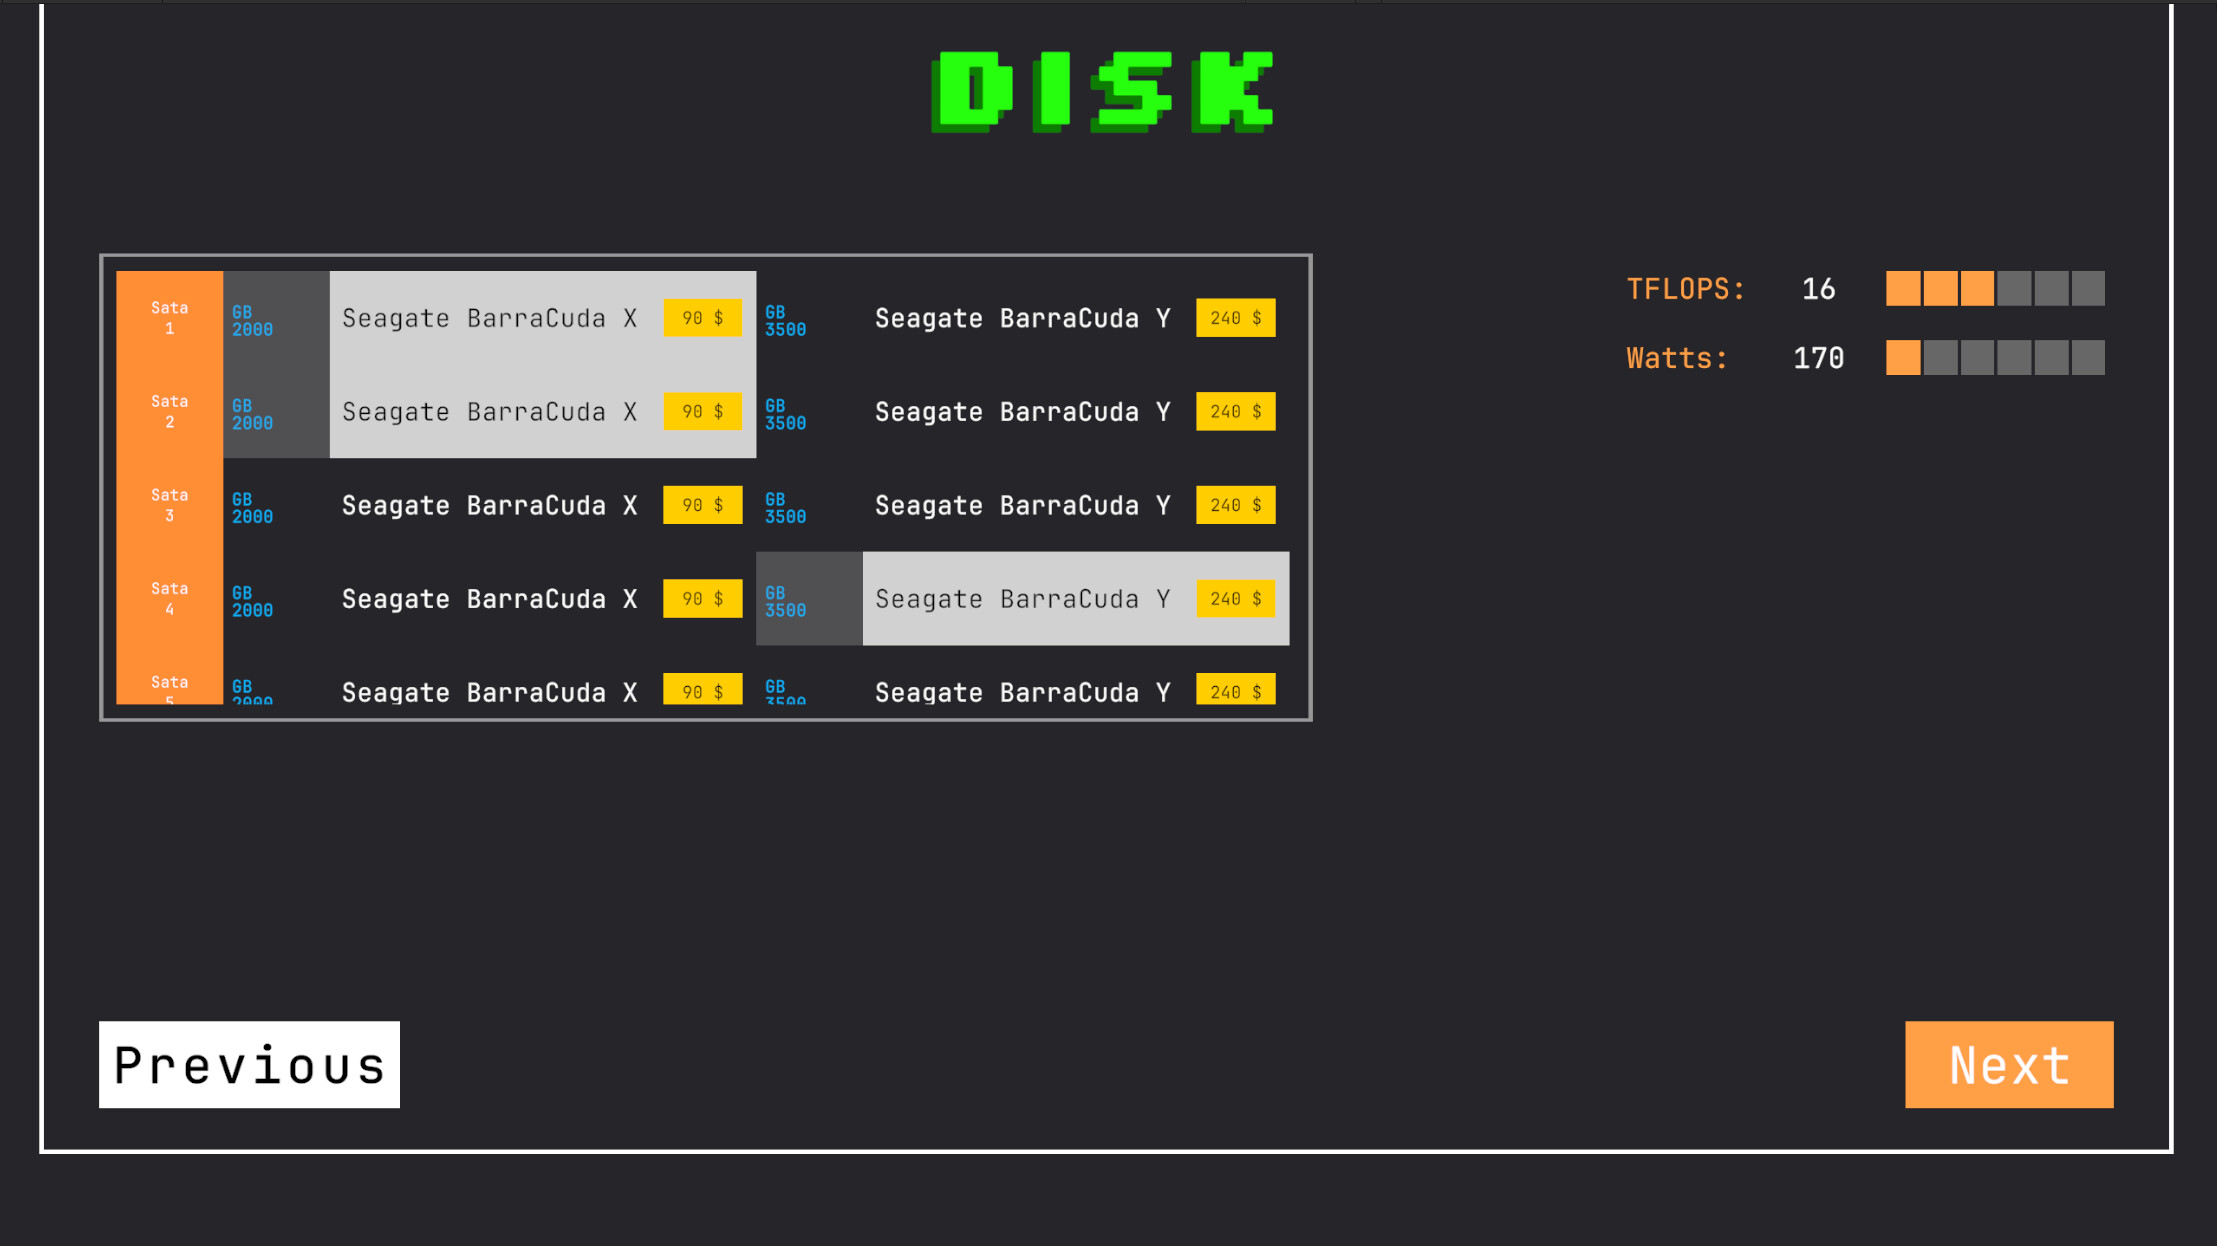
\includegraphics[width=\textwidth]{images/Projeto Disk.jpg}
    \caption[Captura de tela do jogo - Configuração de discos.]{Captura de tela do jogo - Configuração de discos.}
    \label{Projeto_config_disk1}
  \end{minipage}
\end{figure}

Na Figura \ref{Projeto_config_cpu1} e na Figura \ref{Projeto_config_disk1} 
é possível observar a interface de configuração de CPU e de discos, 
respetivamente, onde o jogador tem a possibilidade de escolher entre vários tipos 
de componentes, cada um com as suas próprias características e preços, 
o que torna a escolha do equipamento uma parte importante da estratégia do jogo.
Além disso, cada componente tem um impacto direto no consumo de energia (\textit{Watts})
assim como no desempenho daquele servidor (\textit{TFLOPS}).
As unidades utilizadas (\textit{Watts} e \textit{TFLOPS}) são unidades reais,
e o uso server para reforma a imersão do jogador, além de tornar o jogo mais
realista, e permitir a adição de conteúdo educativo de forma lúdica. 

\subsection{Sistema de economia}

O jogo integra um sistema de economia dinâmico que exige ao utilizador a 
gestão estratégica de recursos financeiros. Esta gestão abrange não só o 
investimento em bens de capital --- como a aquisição de equipamentos e 
respetivos \textit{upgrades} --- mas também a administração de despesas 
operacionais correntes, nomeadamente os custos associados ao consumo de 
eletricidade, sistemas de refrigeração, abastecimento de água e serviços de
 conectividade à internet.

A componente económica é processada em tempo real, mantendo a continuidade 
do fluxo financeiro independentemente do estado da sessão do jogador. Este 
mecanismo assegura que:

\begin{itemize}
    \item \textbf{Débitos Operacionais:} As despesas fixas e variáveis são calculadas com base em períodos predefinidos ($x$ minutos). Caso o jogador se ausente do jogo por um período $n \cdot x$ (onde $n \geq 1$), o montante debitado será igual a n, da próxima vez que abrir o jogo.
    \item \textbf{Fluxos de Rendimento:} De igual modo, a geração de receita é contínua para serviços de subscrição ou fidelização. Um exemplo prático é o aluguer de infraestrutura de \textit{data center} para alojamento de \textit{websites}, onde os ganhos são contabilizados proporcionalmente ao tempo decorrido, garantindo a persistência económica do ecossistema.
\end{itemize}

Este sistema está presente na versão apresentada do projeto, embora com uma
redução no número de variáveis a gerir, tais como a ausência de custos relacionados
com sistema de refrigeração, abastecimento de água e serviços de internet.
Sendo assim as únicas despesas presentes sendo:
\begin{itemize}
    \item Custos relacionados com o consumo de eletricidade;
    \item Custos relacionados com a compra de equipamentos.
\end{itemize}

Todavia, creio que o sistema de economia presente cumpre a função de transmitir
a ideia real de gestão de recursos, além de proporcionar um gancho de interesse para
o jogador voltar a entrar no jogo, com o intuito de receber os pagamentos pendentes.

\subsection{Sistema de combate}

O conceito do jogo conta com uma componente de combate, onde o jogador teria
a sua disposição um sistema de combate e \textit{buids} semelhantes a jogos de \ac{RPG},
mas adaptado ao contexto do jogo. Ou seja, os atributos de ataque, defesa,
velocidade, etc, seriam substituídos por atributos relacionados com o 
contexto do jogo, como, por exemplo, poder de processamento, largura de banda,
algoritmos de segurança, etc...

A intenção desta componente de combate, seria quebrar um pouco do ciclo de jogo,
e proporcionar ao jogador uma experiência mais dinâmica e variada, utilizando da temática
para construir uma experiência diferente e divertida, onde o jogador
poderia ser introduzido a conceitos e expressões técnicas de uma forma lúdica
sem perder o foco na diversão.

Segundo \textcite{bogost}, os jogos não comunicam apenas por imagens ou palavras, mas por meio de processos. Ou seja, quando utiliza de 
um contexto de Data Center adaptado a um \ac{RPG}, estamos a criar 
um modelo de como esse sistema funciona. Segundo o autor, essa 
"aprendizagem por simulação" gera uma curiosidade intrínseca, 
pois o jogador tenta decifrar a lógica do sistema real através 
das regras do jogo.

Embora a ideia apresentada a cima seria a ideal para o conceito do jogo, infelizmente
devido a sua complexidade para o seu desenvolvimento, o projeto apresentado teve de ser
adaptado, no sentido em que vês de ter o sistema de \ac{RPG}, o jogo terá uma
metralhadora no cenário em que o jogador terá de a usar para destruir os inimigos (vírus e \textit{hackers}), representados sobre a forma de \textit{drones},
que iram aparecer durante momentos da \textit{gameplay}.
Embora, essa adaptação carece em termos de complexidade e profundidade de contexto,
limitando a precessão do jogador comparado com o sistema de \ac{RPG}, creio mesmo assim
ser relevante uma vez que introduz um elemento de combate, e quebra uma pouco do ciclo de jogo,
que se poderia tornar repetitivo, além de proporcionar uma experiência mais dinâmica e divertida para o jogador.

\subsection{Estilo e estética}

O jogo é caracterizado por ser um jogo 3D com uma perspetiva isométrica, onde 
o jogador tem uma visão geral do cenário, e pode interagir com os diferentes 
elementos do jogo para cumprir os objetivos propostos.

O jogo faz uso de elementos de fantasia e ficção, principalmente na estética, visando criar um ambiente mais divertido e envolvente para o jogador.

\section{\textit{Gameplay Loops}}

Um \textit{gameplay loop} é ciclo de ações que se repete, sendo tipicamente composto por 3 etapas:
\begin{itemize}
    \item Objetivo;
    \item Desafio;
    \item Recompensa;
\end{itemize}
que definem a experiência do jogo.
Estes ciclos estão presentes em várias partes do projeto desenvolvido, tais como na compra de equipamentos, resolução de tarefas(pedidos de clientes) e combate.

Posto isto, nas subsecções seguinte serão apresentados o core \textit{gameplay loop}, assim como os \textit{gameplays} secundário.

\subsection{\textit{Gameplay loop}}

\begin{figure}[H]
    \centering
    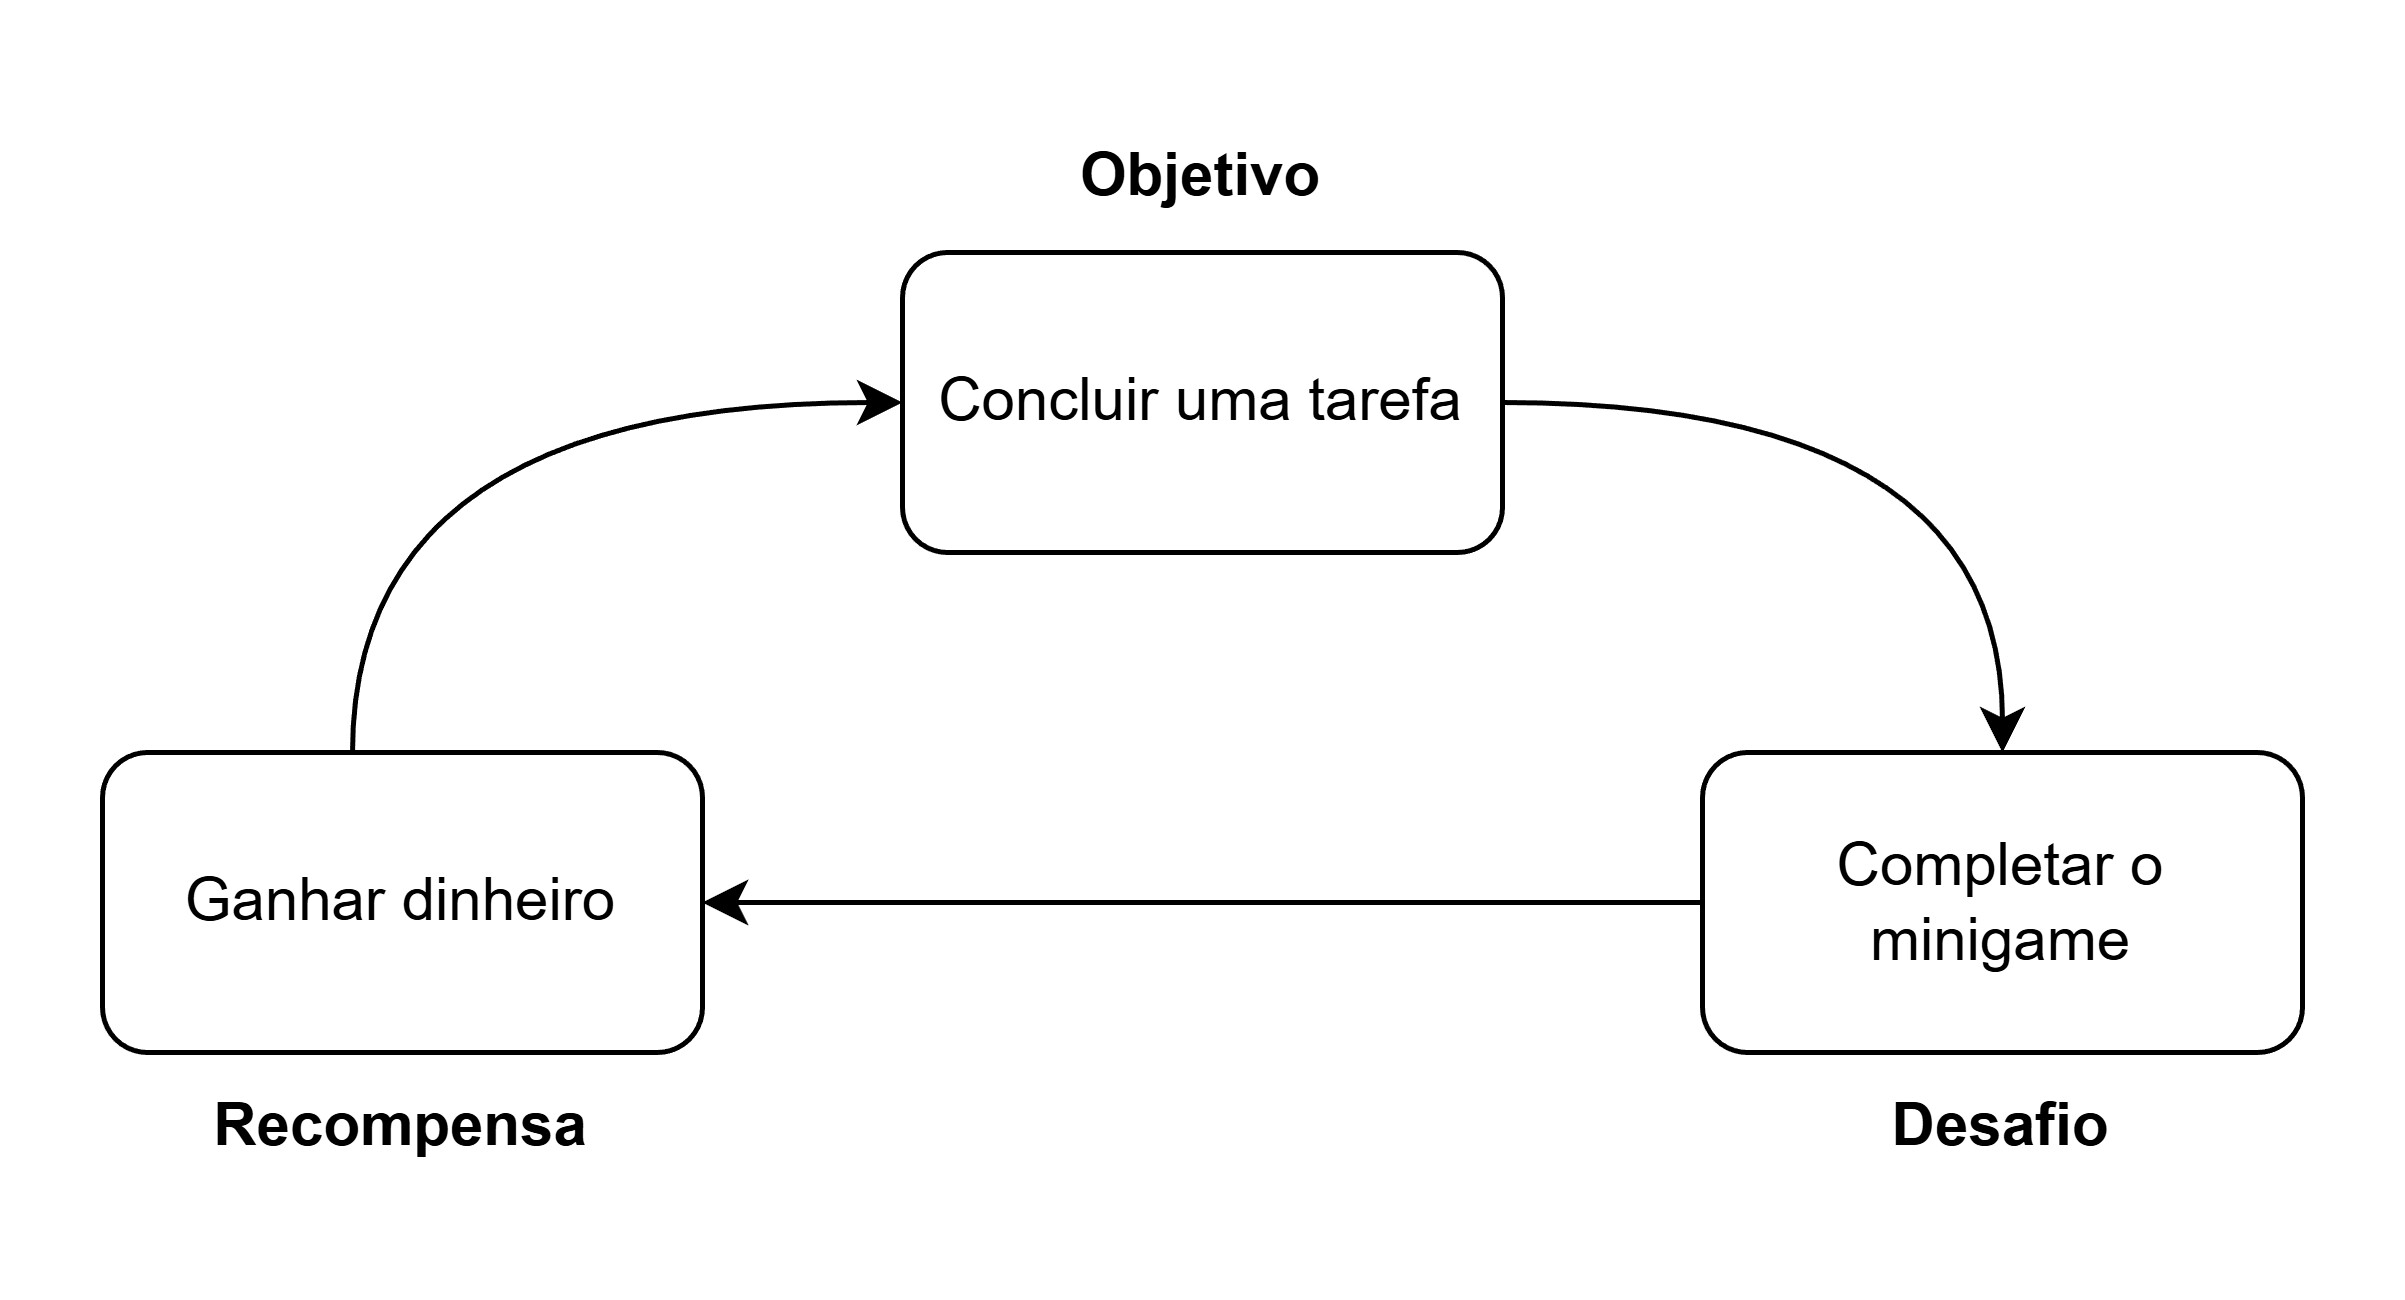
\includegraphics[width=0.9\textwidth]{Diagramas/Core_Gameplay_Loop.jpg}
    \caption{Diagrama do \textit{core gameplay loop} do jogo desenvolvido.}
    \label{Core_Gameplay_Loop}
\end{figure}

A Figura \ref{Core_Gameplay_Loop} apresenta o diagrama do \textit{core gameplay loop}, ou seja, o ciclo de ações principais do jogo.
A tarefa referida no diagrama, diz respeito aos pedidos dos clientes. Esses pedidos aparecem de forma constante e periódica durante toda a \textit{gameplay} além de representarem a principal forma do jogador conseguir dinheiro.

\newpage

A seguir apresenta-se os \textit{gameplay loops} secundários, ou seja, os ciclos de ações relacionados com a compra e configuração de equipamentos, e o ciclo de ações relacionado com o combate.

\begin{figure}[H]
    \centering
    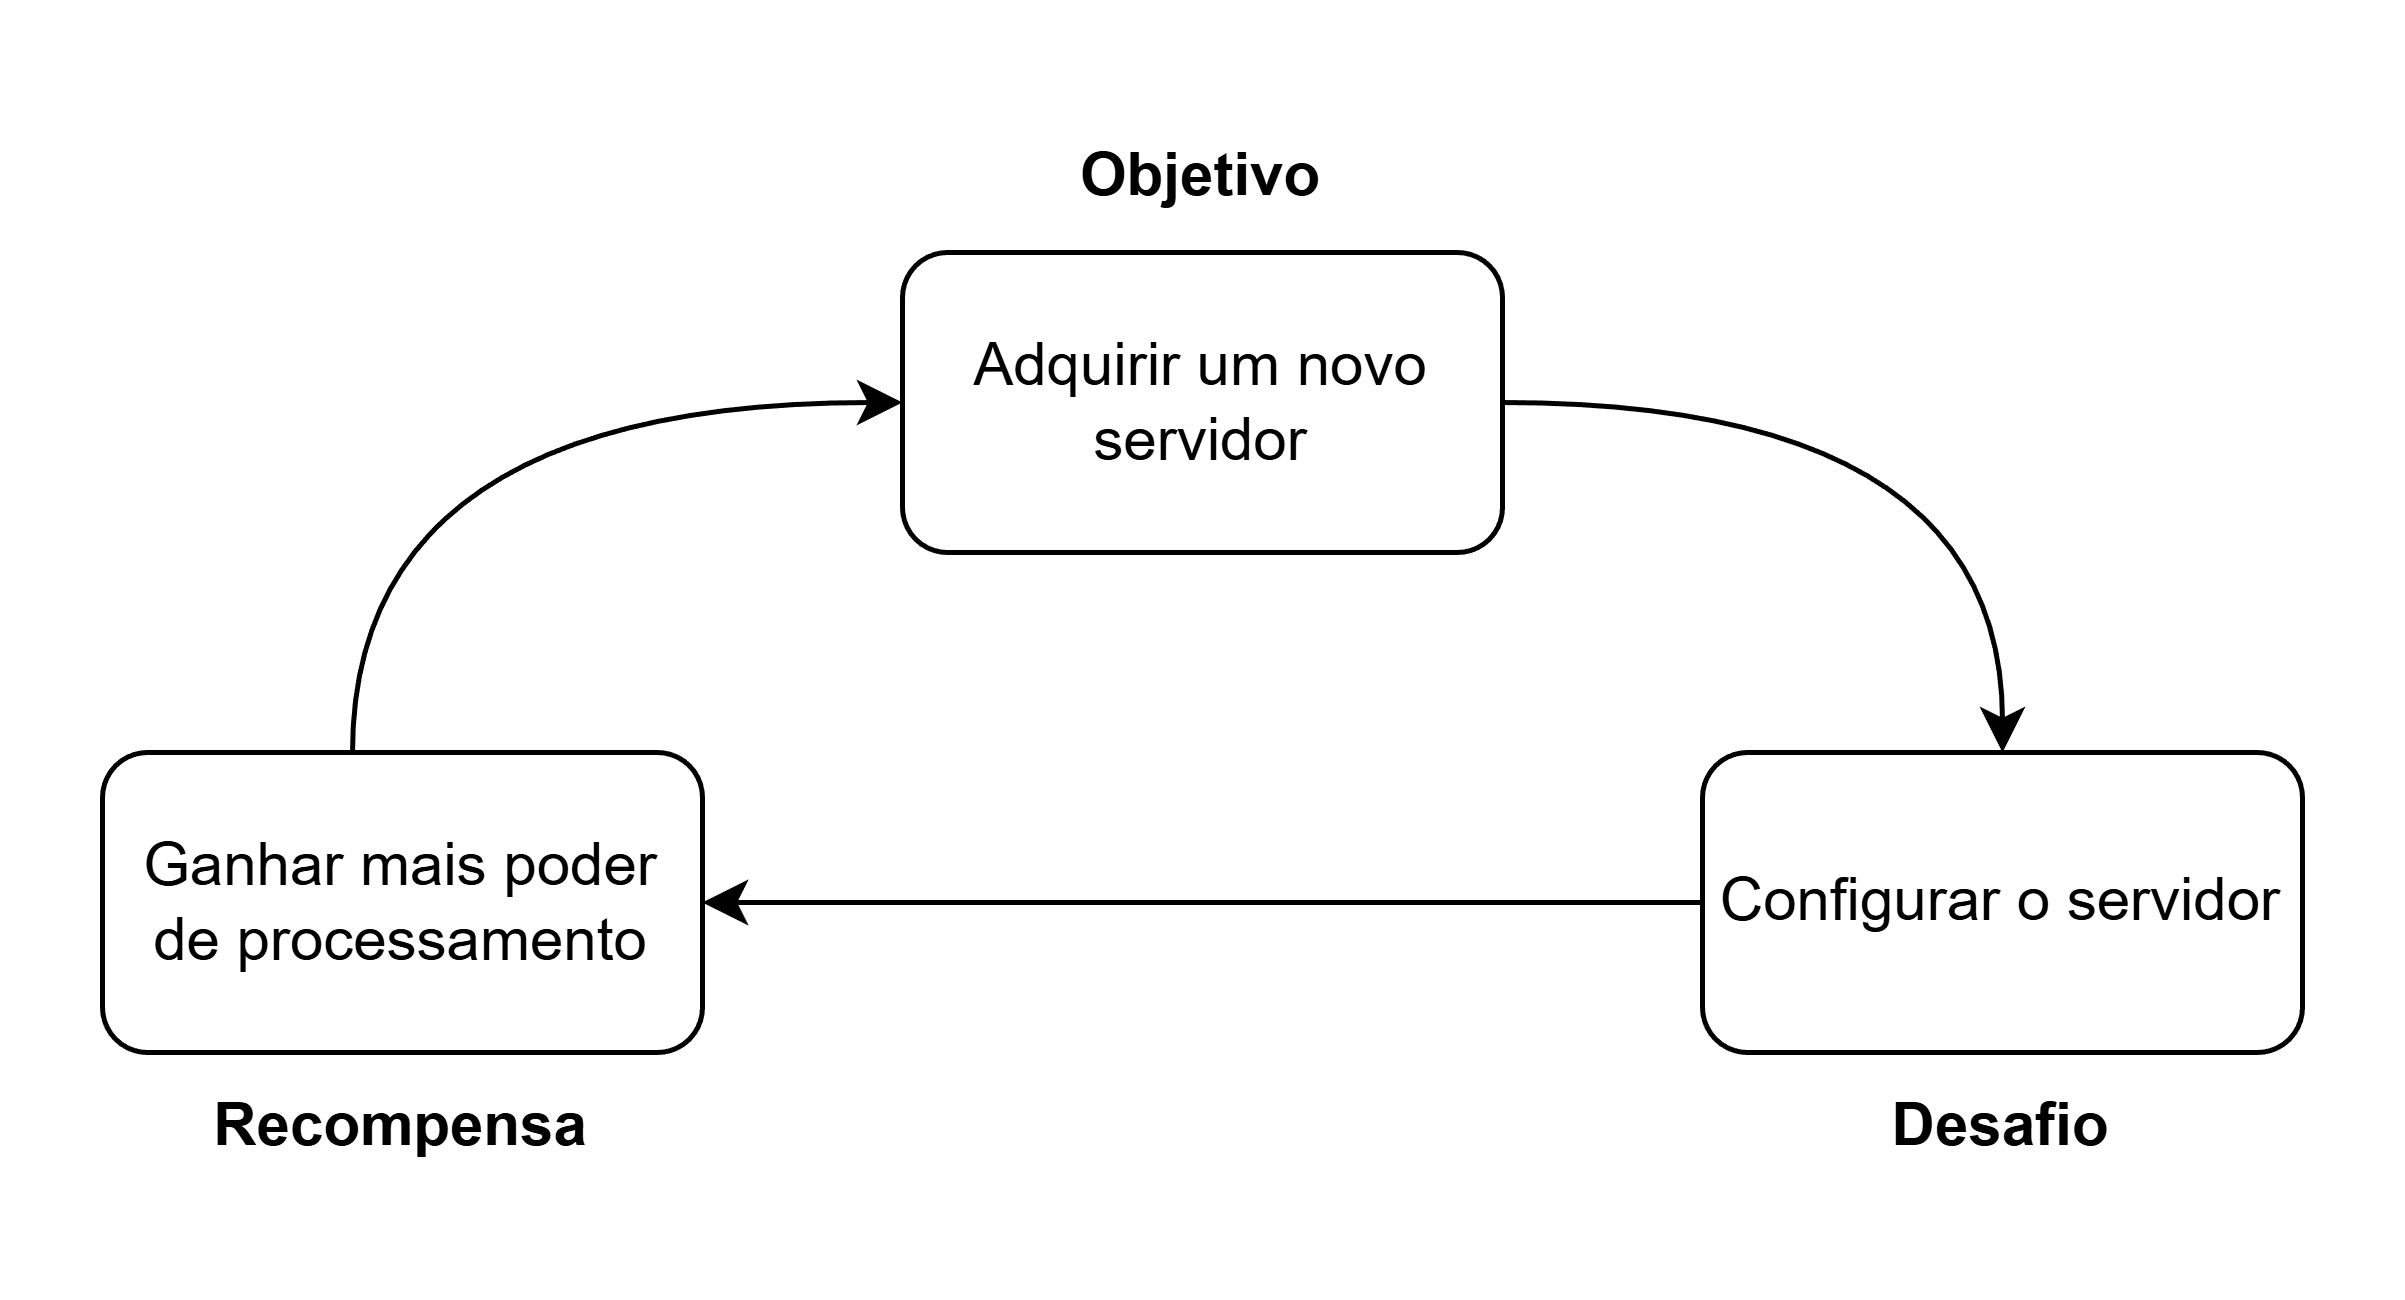
\includegraphics[width=0.9\textwidth]{Diagramas/Shop_Gameplay_Loop.png}
    \caption{Diagrama do \textit{gameplay loop} referente à configuração de servidores.}
    \label{Servers_Gameplay_Loop}
\end{figure}


\begin{figure}[H]
    \centering
    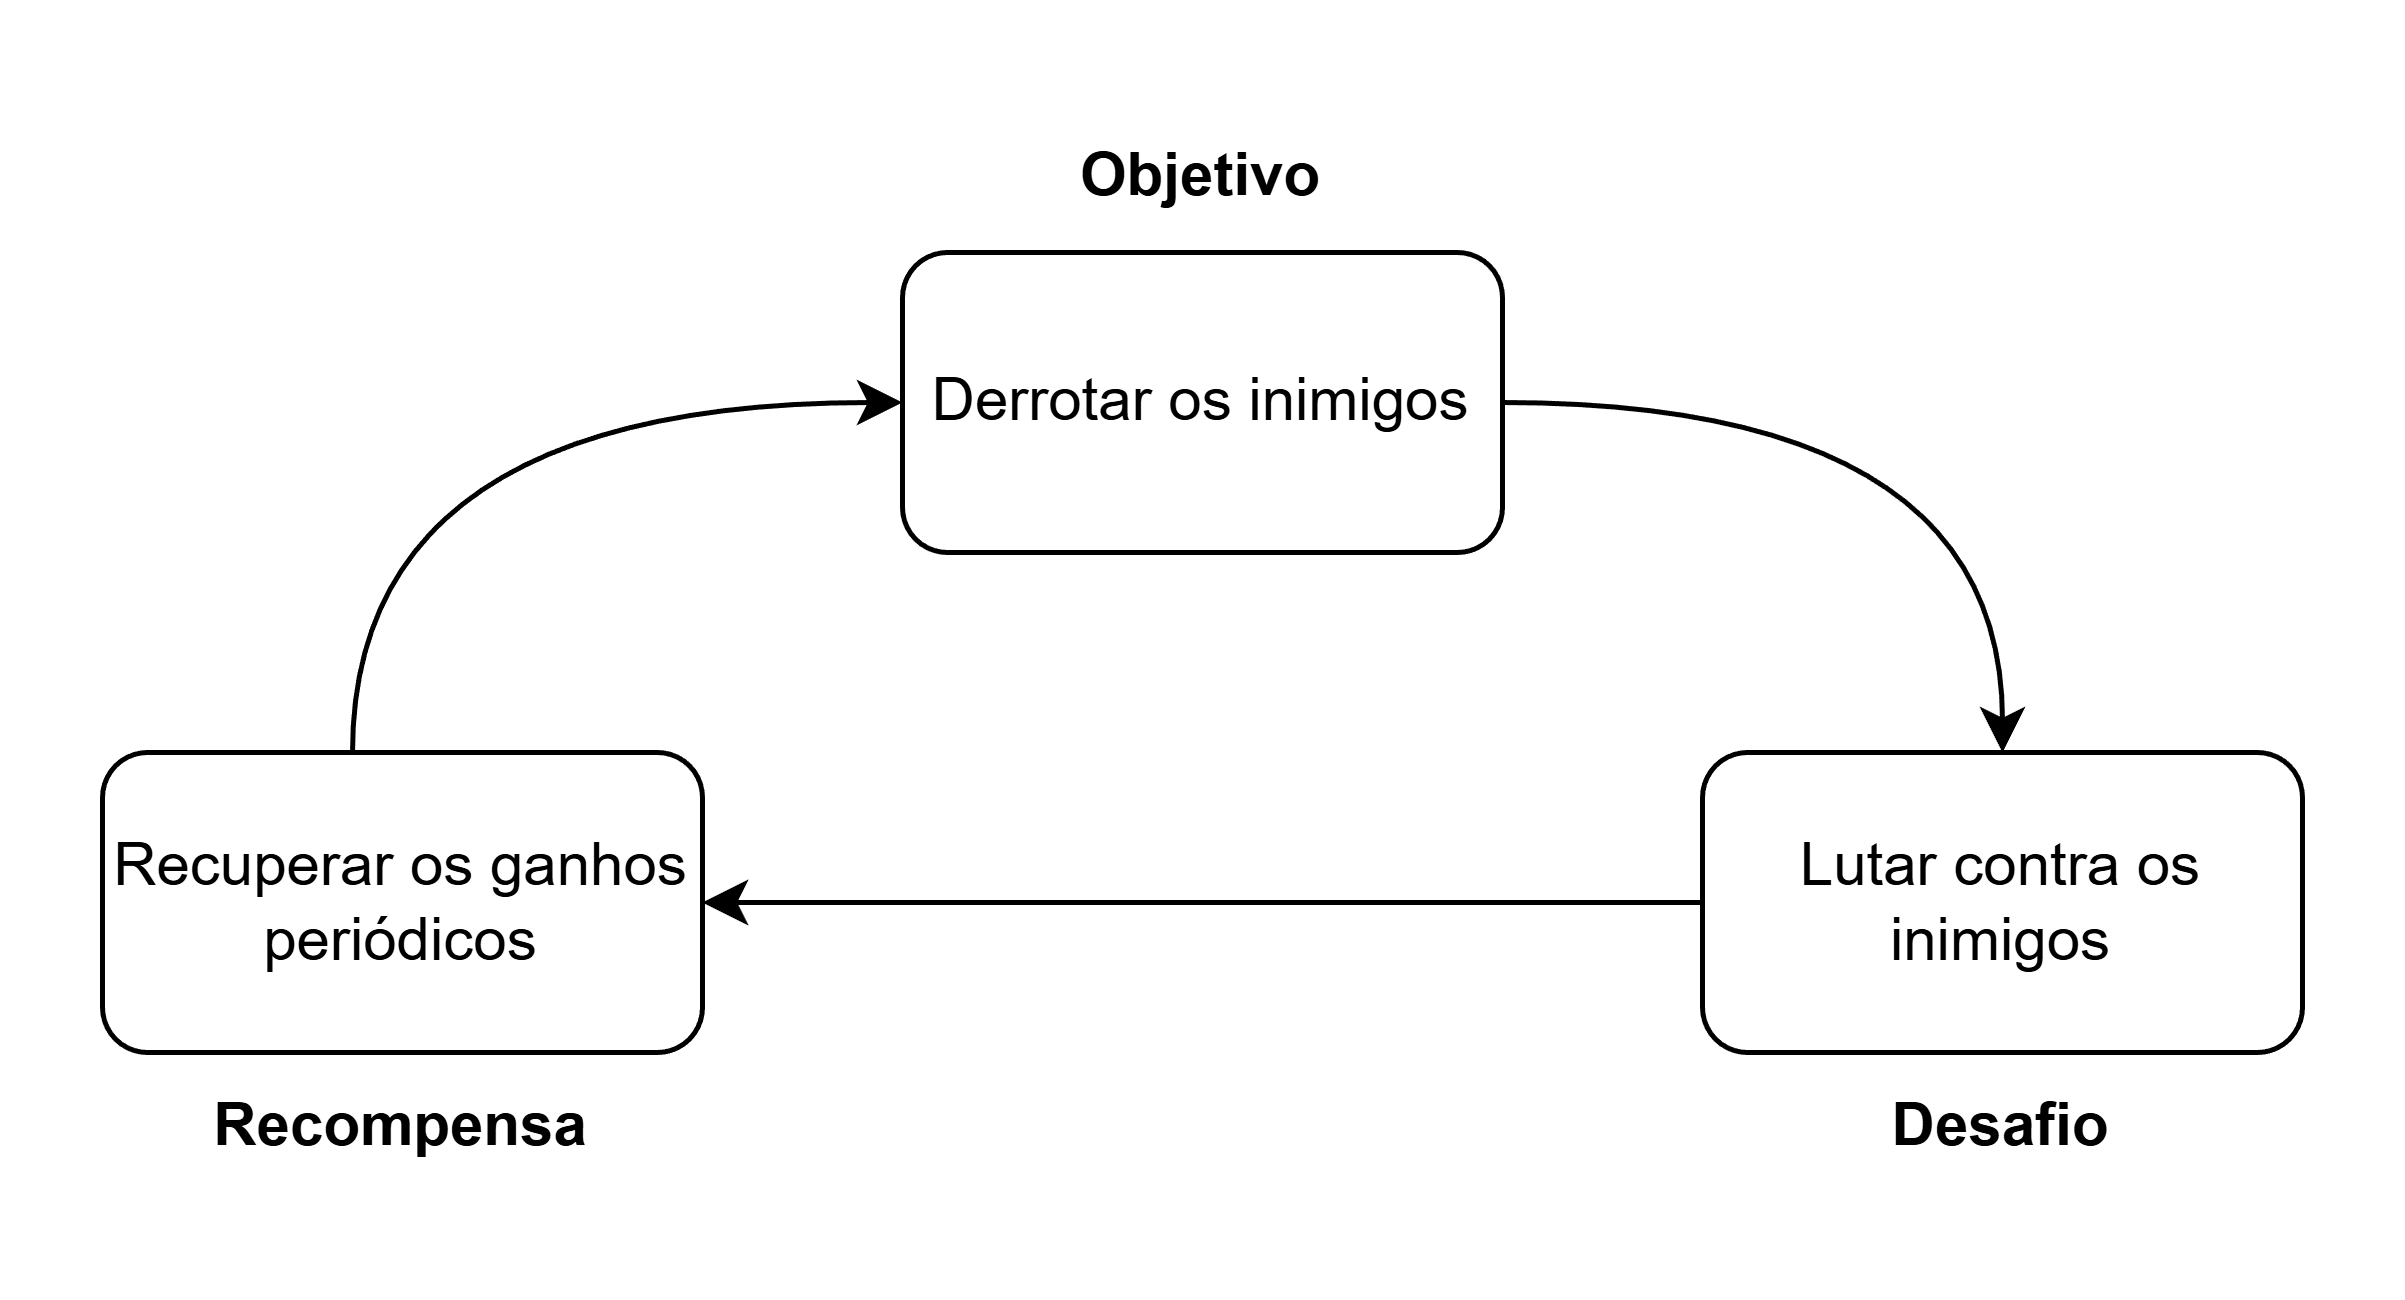
\includegraphics[width=0.9\textwidth]{Diagramas/Combat_Gameplay_Loop.png}
    \caption{Diagrama do \textit{gameplay loop} referente ao combate.}
    \label{Combat_Gameplay_Loop}
\end{figure}




%\setcounter{secnumdepth}{+2}
\chapter{Implementação do Jogo}
%\chapter{Design and Development}
\label{cap4}

\section{Ferramentas e Tecnologias Utilizadas}

Várias ferramentas e diferentes tecnologias, foram utilizadas durante todo o processo de
desenvolvimento deste projeto, permitindo assim o seu desenvolvimento e facilitando a usa
implementação. Considerando ferramentas de construção de conteúdo digital até linguagens de programação.
Posto isto, as ferramentas e tecnologias utilizadas foram:

\begin{itemize}
    \item \textbf{\textcite{Blender}}: \textit{Software} de modelação 3D. Este \textit{software} foi utilizado para a modelação completa do cenário, assim como para a realização de ajuste no personagem (Criação de textura);
    \item \textbf{\textcite{Unity}}: \textit{Game Engine}, \textit{software} principal para o desenvolvimento do projeto. Ele é responsável pela junção dos \textit{asset's} com o código. Permitindo assim a construção de um experiência interativa. Além de ser utilizado para a criação de \textit{shaders}, que influenciam na construção visual do projeto;
    \item \textbf{Chat 3D:} Ferramenta de \ac{IA}. Utiliza para desenvolver o modelo 3D do personagem do jogo utilizando imagens 2D como base para a sua criação;
    \item \textbf{Gemini (Nano banana):} Ferramenta de \ac{IA}, utilizada para desenvolver o conceito do personagem, assim como utilizada para a criação de imagens ilustrativas do mesmo, que foram utilizadas no Chat 3D;
    \item \textbf{Processing:} \textit{Framework} de Java, que permite a a criação de imagens 2D. Esta tecnologia foi utilizada para a criação de algumas das partículas 2D presentes na \ac{UI}.;
    \item \textbf{Gimp e Affinity:} Ferramentas de edição de imagem. Foram utilizadas principalmente para ajustar as imagens geradas pelo Gemini;
    \item \textbf{C\#:} Linguagem de programação principal. É utilizada para a construção completa do jogo dentro da Unity. Responsável pela lógica do jogo, assim como implementação de sistema de \textit{gameplay};
    \item \textbf{Java:} Linguagem de programação utilizada no \textit{framework} Processing. Utilizada para a construção de certos \textit{assets} 2D;
\end{itemize}

\newpage

\section{Engenharia de Software}

\subsection{Diagrama de sistema de jogo}
\label{Sec:DiagramaSistemaJogo}

\begin{figure}[H]
    \centering
    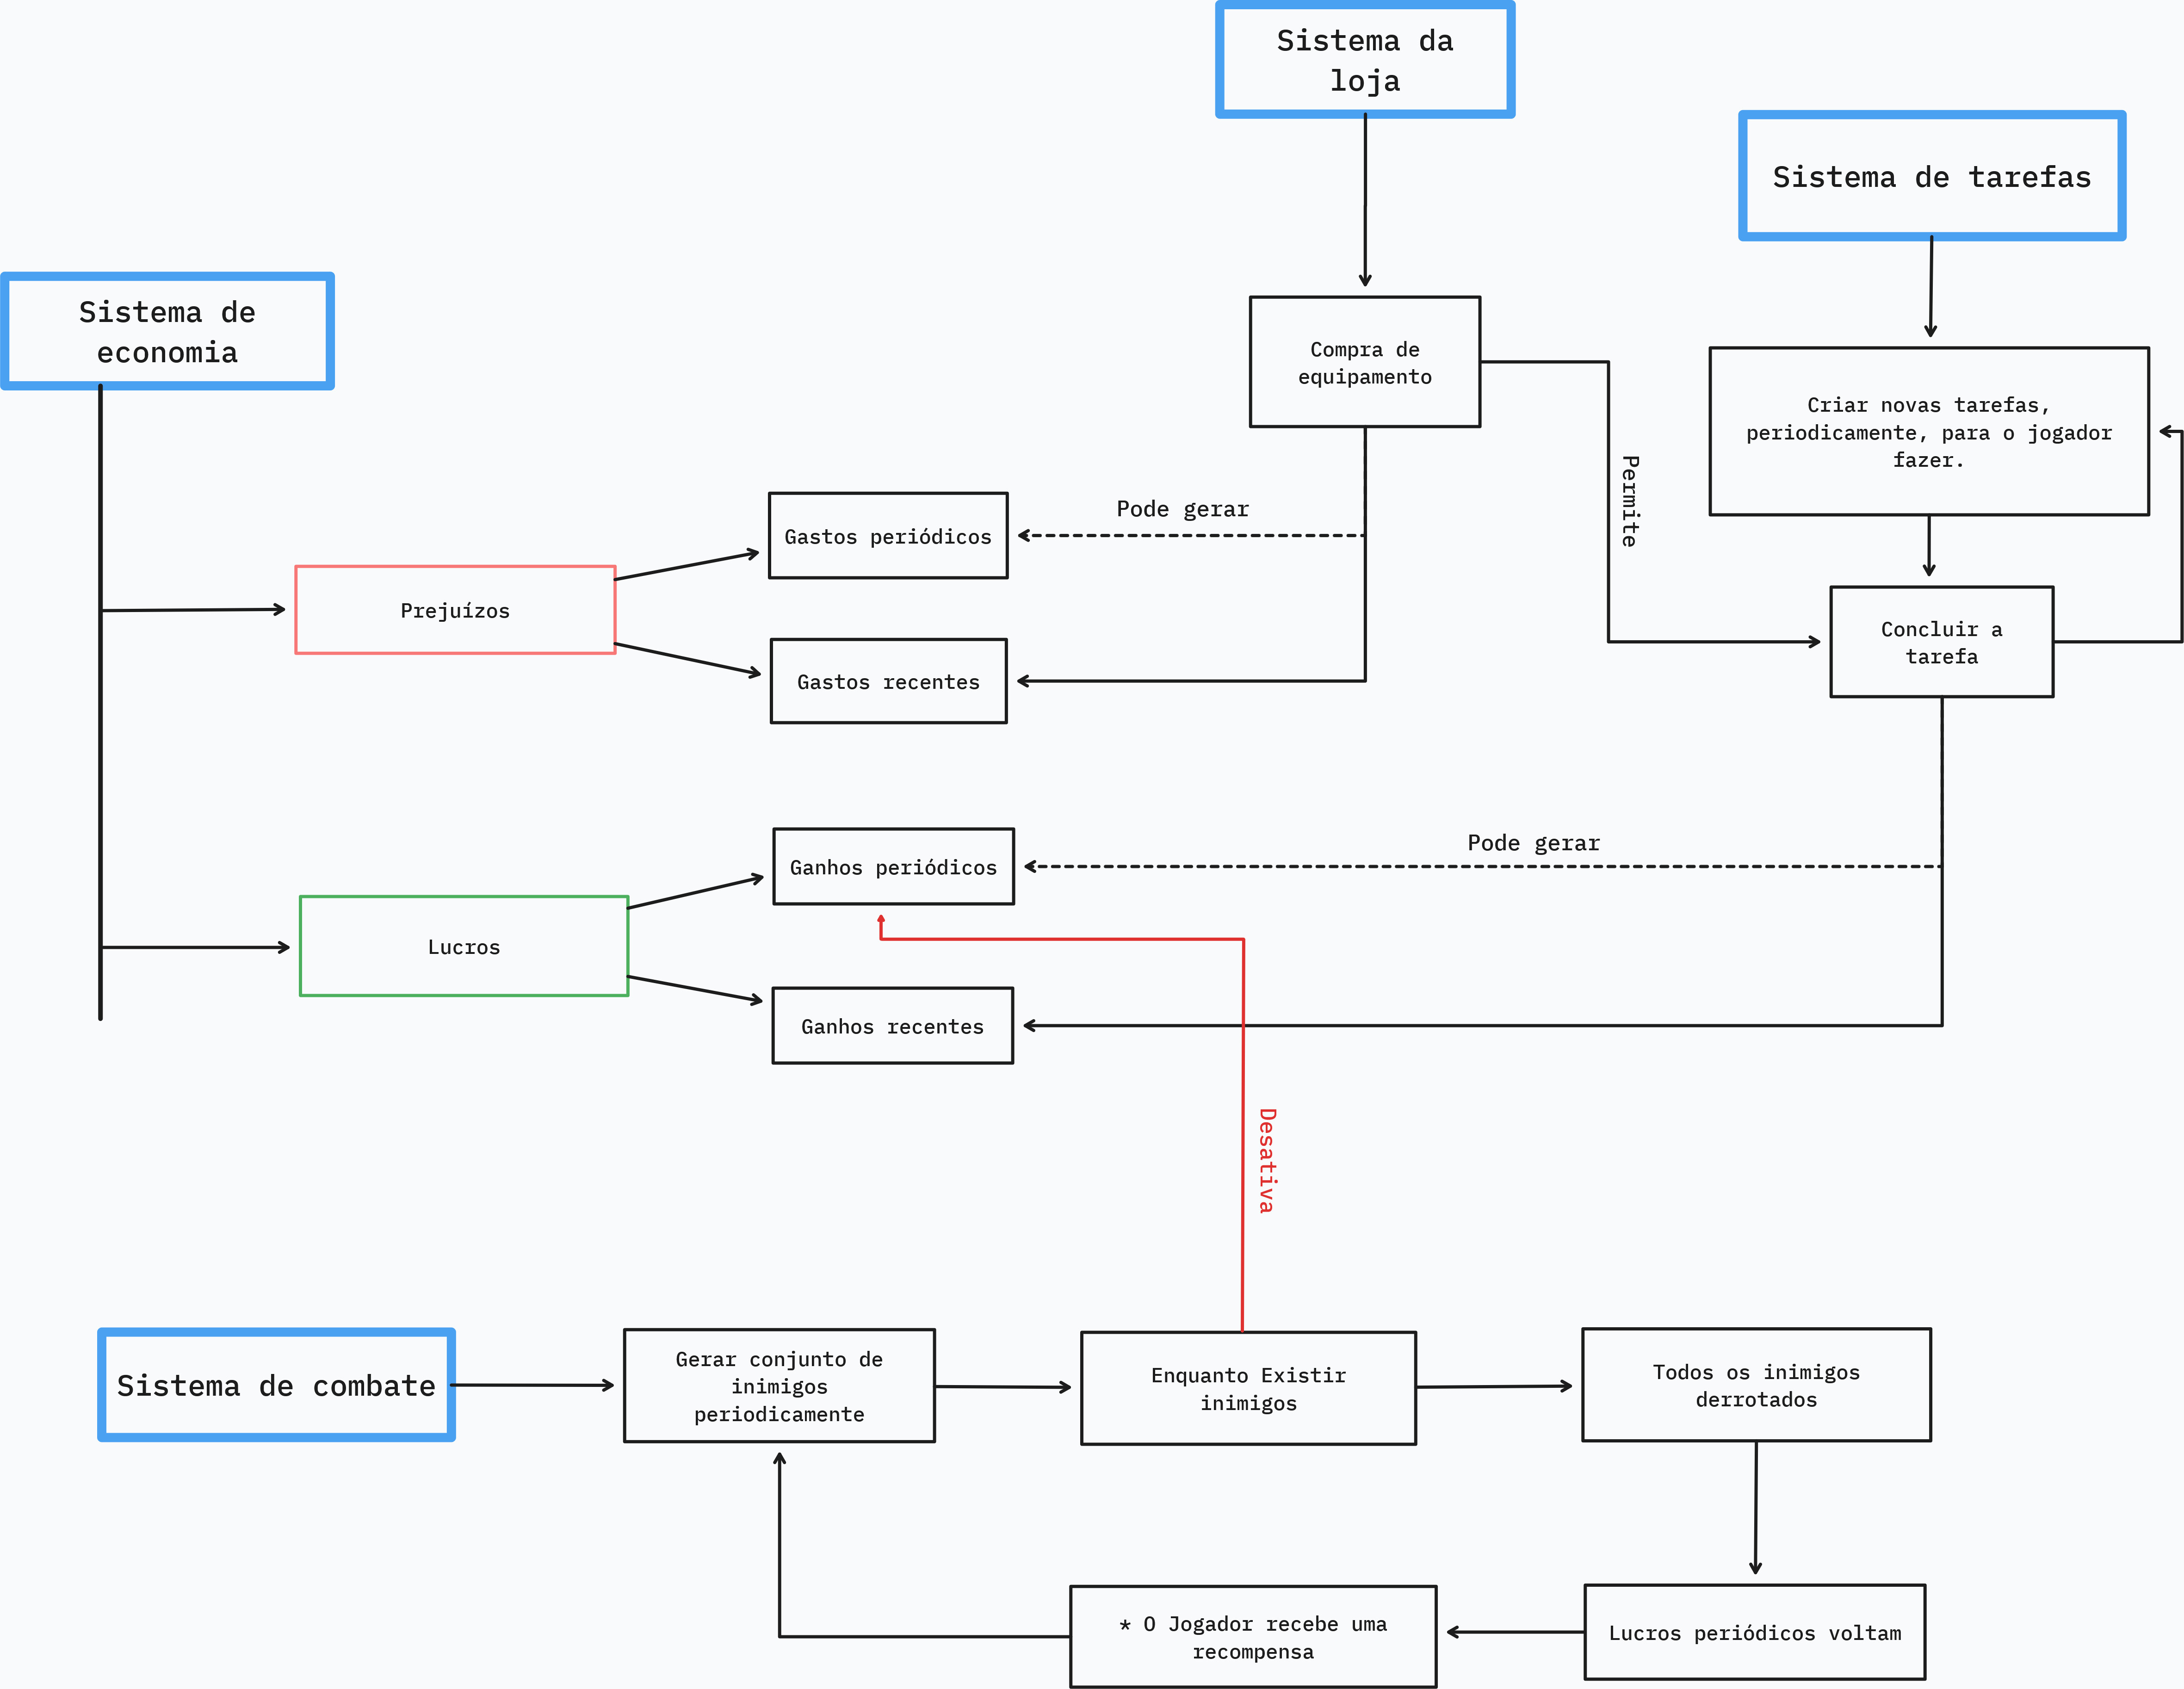
\includegraphics[width=1\textwidth]{Diagramas/diagrama_game.jpg}
    \caption{Diagrama de sistema do jogo.}
    \label{Diagrama_Sistema_Jogo}
\end{figure}

A Figura \ref{Diagrama_Sistema_Jogo} apresenta o diagrama de sistema do jogo, onde é possível observar os vários sistemas que compõem o jogo, assim como a interação entre eles.
Como é observável, todos os sistemas interagem com o sistema de economia, uma vez que esse sistema está fortemente ligado com a condição de derrota.
Além disso, é observável que o único sistema que permite com que o jogador ganhe dinheiro é o sistema de tarefas, o que faz com que seja através dele que o jogador consiga progredir no jogo, e como tal é o sistema que o jogador interage mais durante o jogo.

No diagrama, é possível observar que no sistema de combate, existe uma recompensa para o jogador.

\newpage

\subsection{Diagramas de caso de uso}
Diagramas de caso de uso, descrevem a funcionalidade de um sistema através da interação entre atores (utilizadores/sistema).
No contexto deste projeto os utilizadores são os jogadores e o sistema são os vários sistemas que compõem o jogo.
Nas subsecções subsequentes serão apresentados os diagramas de caso de uso dos três principais sistemas:
Tarefas, Loja e combate.

\subsubsection{Tarefas}

\begin{figure}[H]
    \centering
    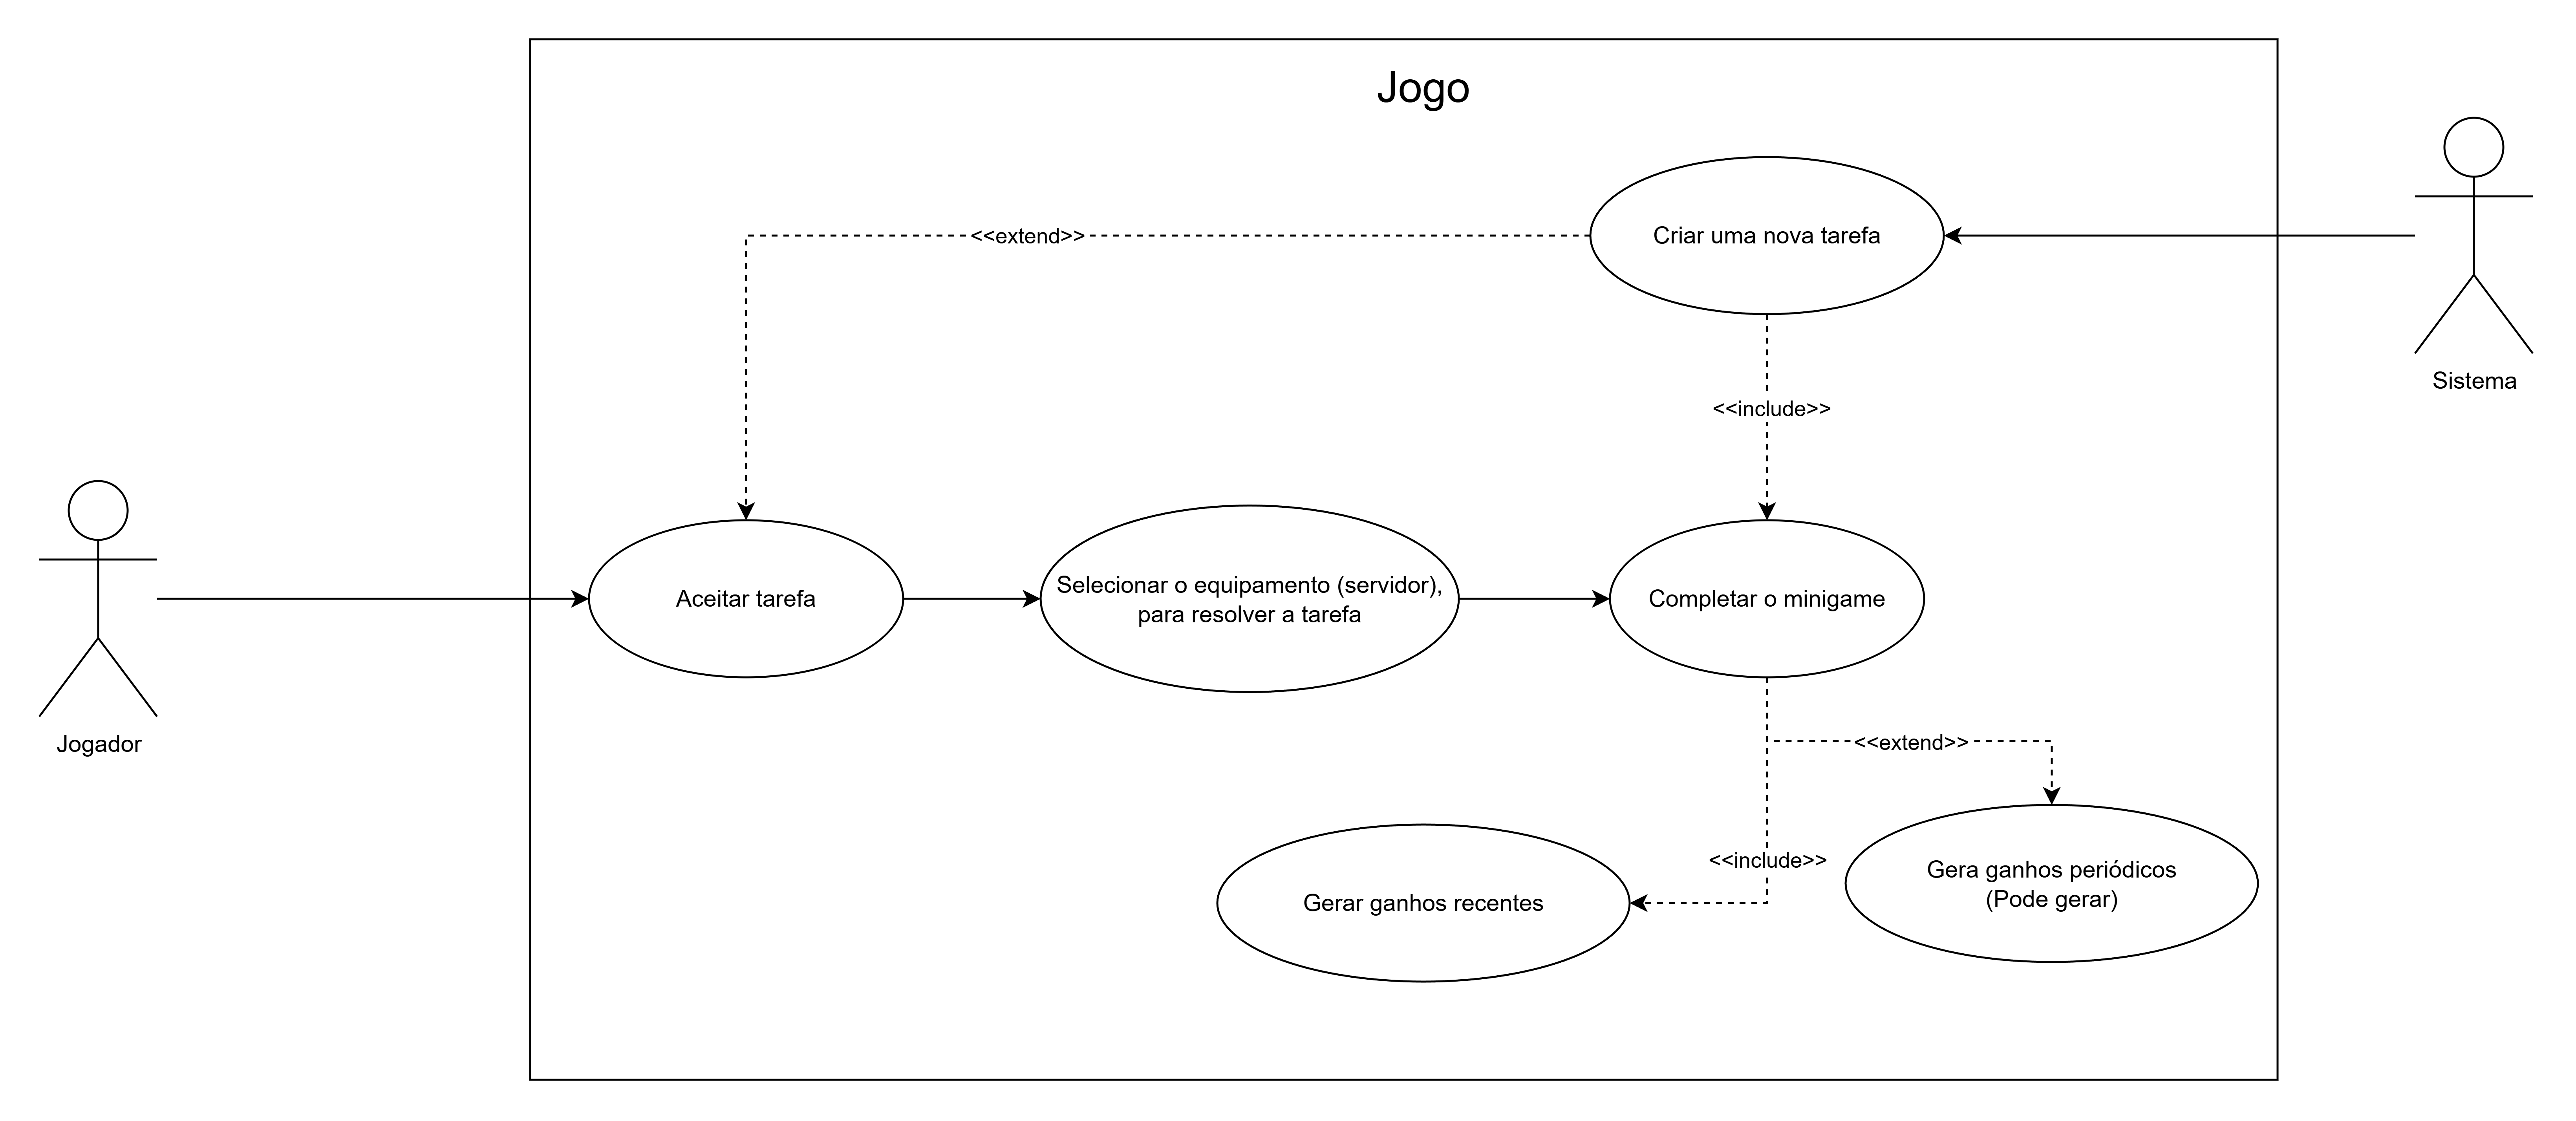
\includegraphics[width=0.9\textwidth]{Diagramas/Use_case_Tarefa.png}
    \caption{Diagrama de Caso de uso - Tarefas}
    \label{User_Case_Quests}
\end{figure}

O diagrama da Figura \ref{User_Case_Quests}, retrata a interação entre o jogador e o sistema de tarefas que periodicamente
cria tarefas para o jogador fazer, as quais, o jogador pode aceitar ou recusar. Uma vez que, cada tarefa
exigi recursos, o jogador pode escolhe recusar uma vez que pode não os ter ou acreditar que não compensa.

Além disso, assim como mostra o diagrama, 
ou concluir cada tarefa o jogador recebe uma certa quantidade de dinheiro,
podendo em certos casos receber outra quantidade de dinheiro de forma periódica.

\subsubsection{Loja}

\begin{figure}[H]
    \centering
    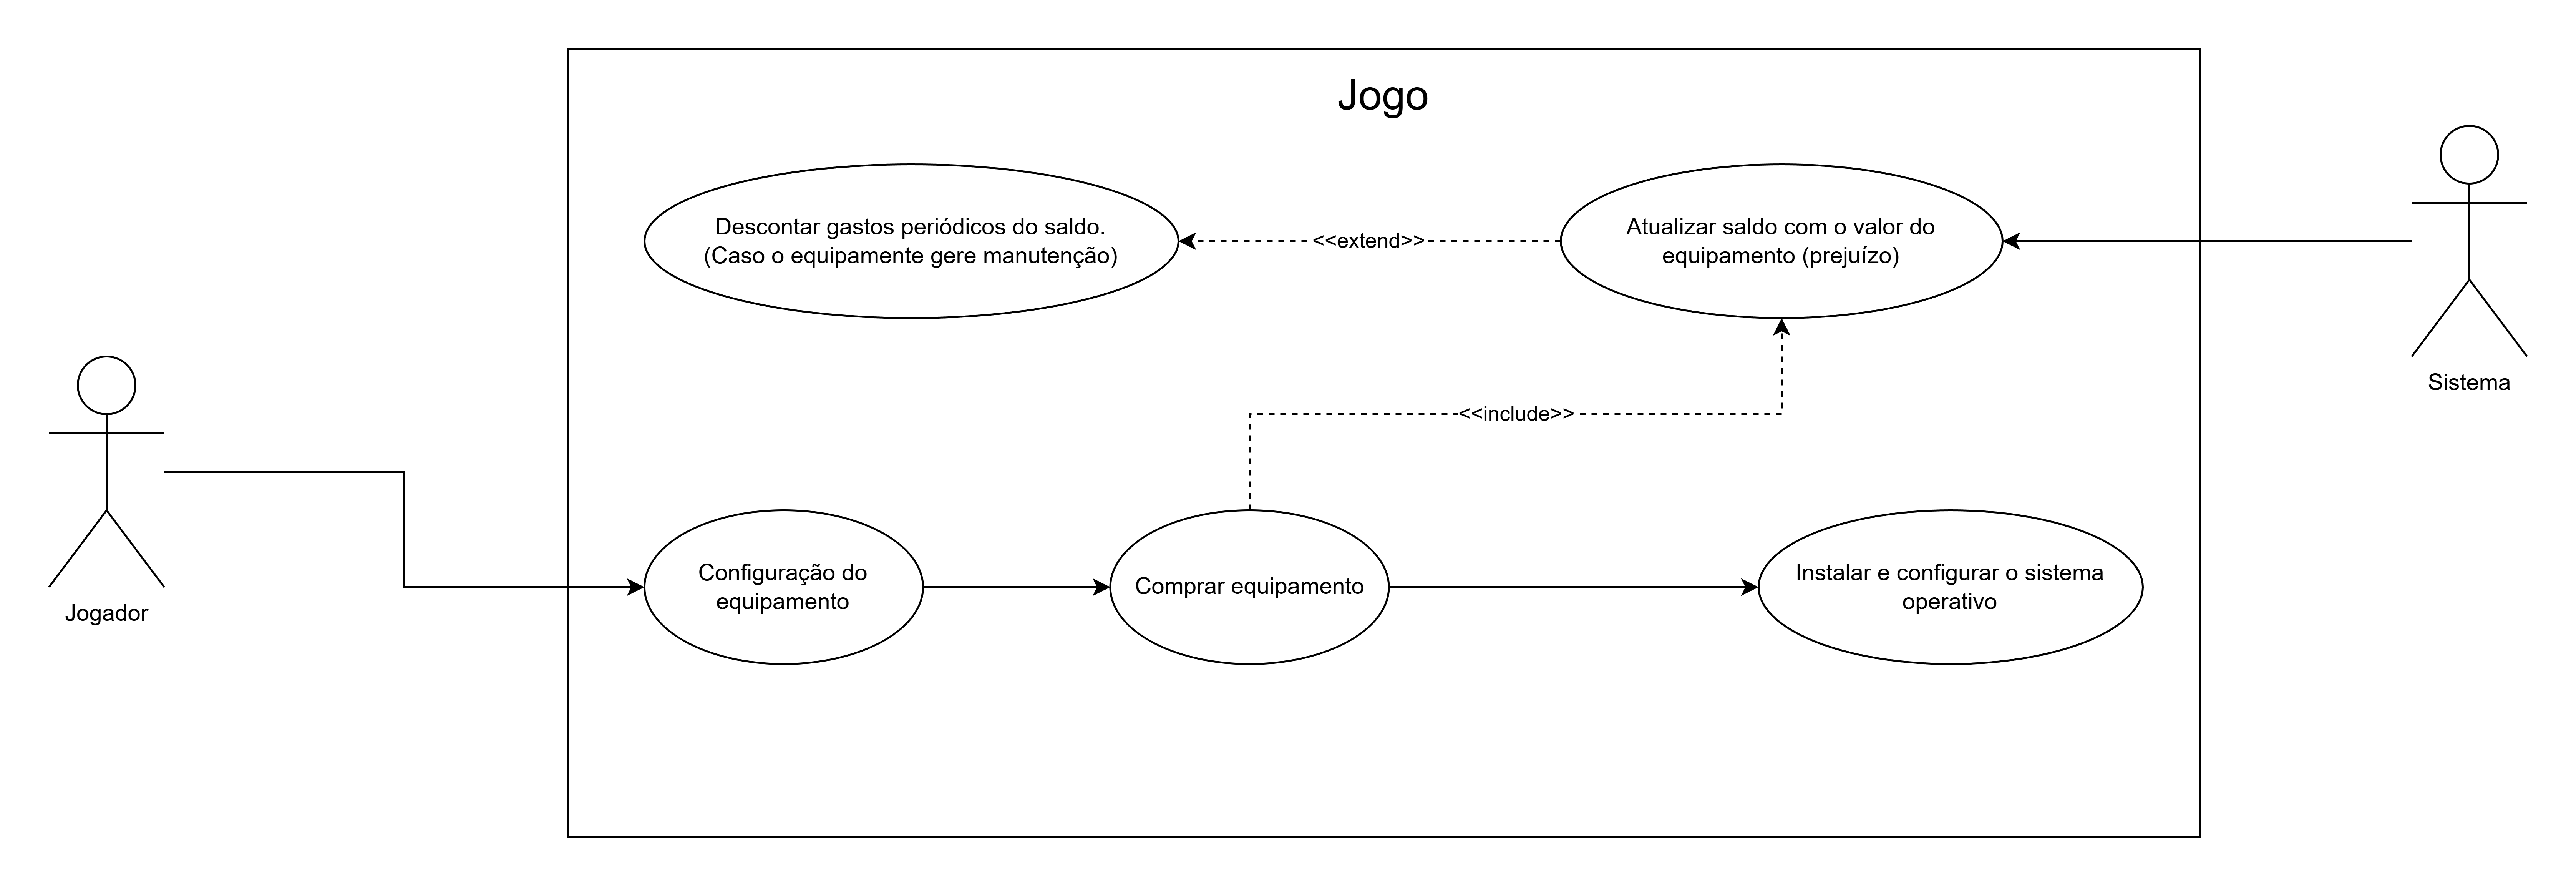
\includegraphics[width=0.9\textwidth]{Diagramas/Use_case_Shop.png}
    \caption{Diagrama de Caso de uso - Loja}
    \label{User_Case_Shop}
\end{figure}

A Figura \ref{User_Case_Shop} ilustra como o jogador interage com o sistema de Loja.
Os pontos mais relevantes das funcionalidades apresentadas são:
\begin{itemize}
    \item \textbf{Configuração de equipamento:} Uma vez que nesta etapa o jogador pode montar o servidor com o equipamento que quiser, dando assim liberdade para que o jogador possa ser criativo e conseguia balancear aspetos relevantes (como performance, armazenamento, refrigeração) face ao custo envolvido.
    \item \textbf{Instalação de sistema operativo:} É um passo à posterior a configuração do equipamento, onde o jogador tem que faz uma simulação de instalação de um sistema operativo, onde pode escolher o nome daquele servidor assim como a \textit{password}. Este passo é importante para a construção da experiência, uma vez que é um processo que acontece na realidade, e que tem um certo grau de complexidade, o que pode ajudar a construir uma experiência mais imersiva. Além disso, o nome atribuído ao servidor, é utilizado posteriormente para o jogador conseguir identificar o seu servidor, uma vez que o jogador pode ter mais do que um servidor.
\end{itemize}

\subsubsection{Combate}
\label{Sec:SistemaCombate}

\begin{figure}[H]
    \centering
    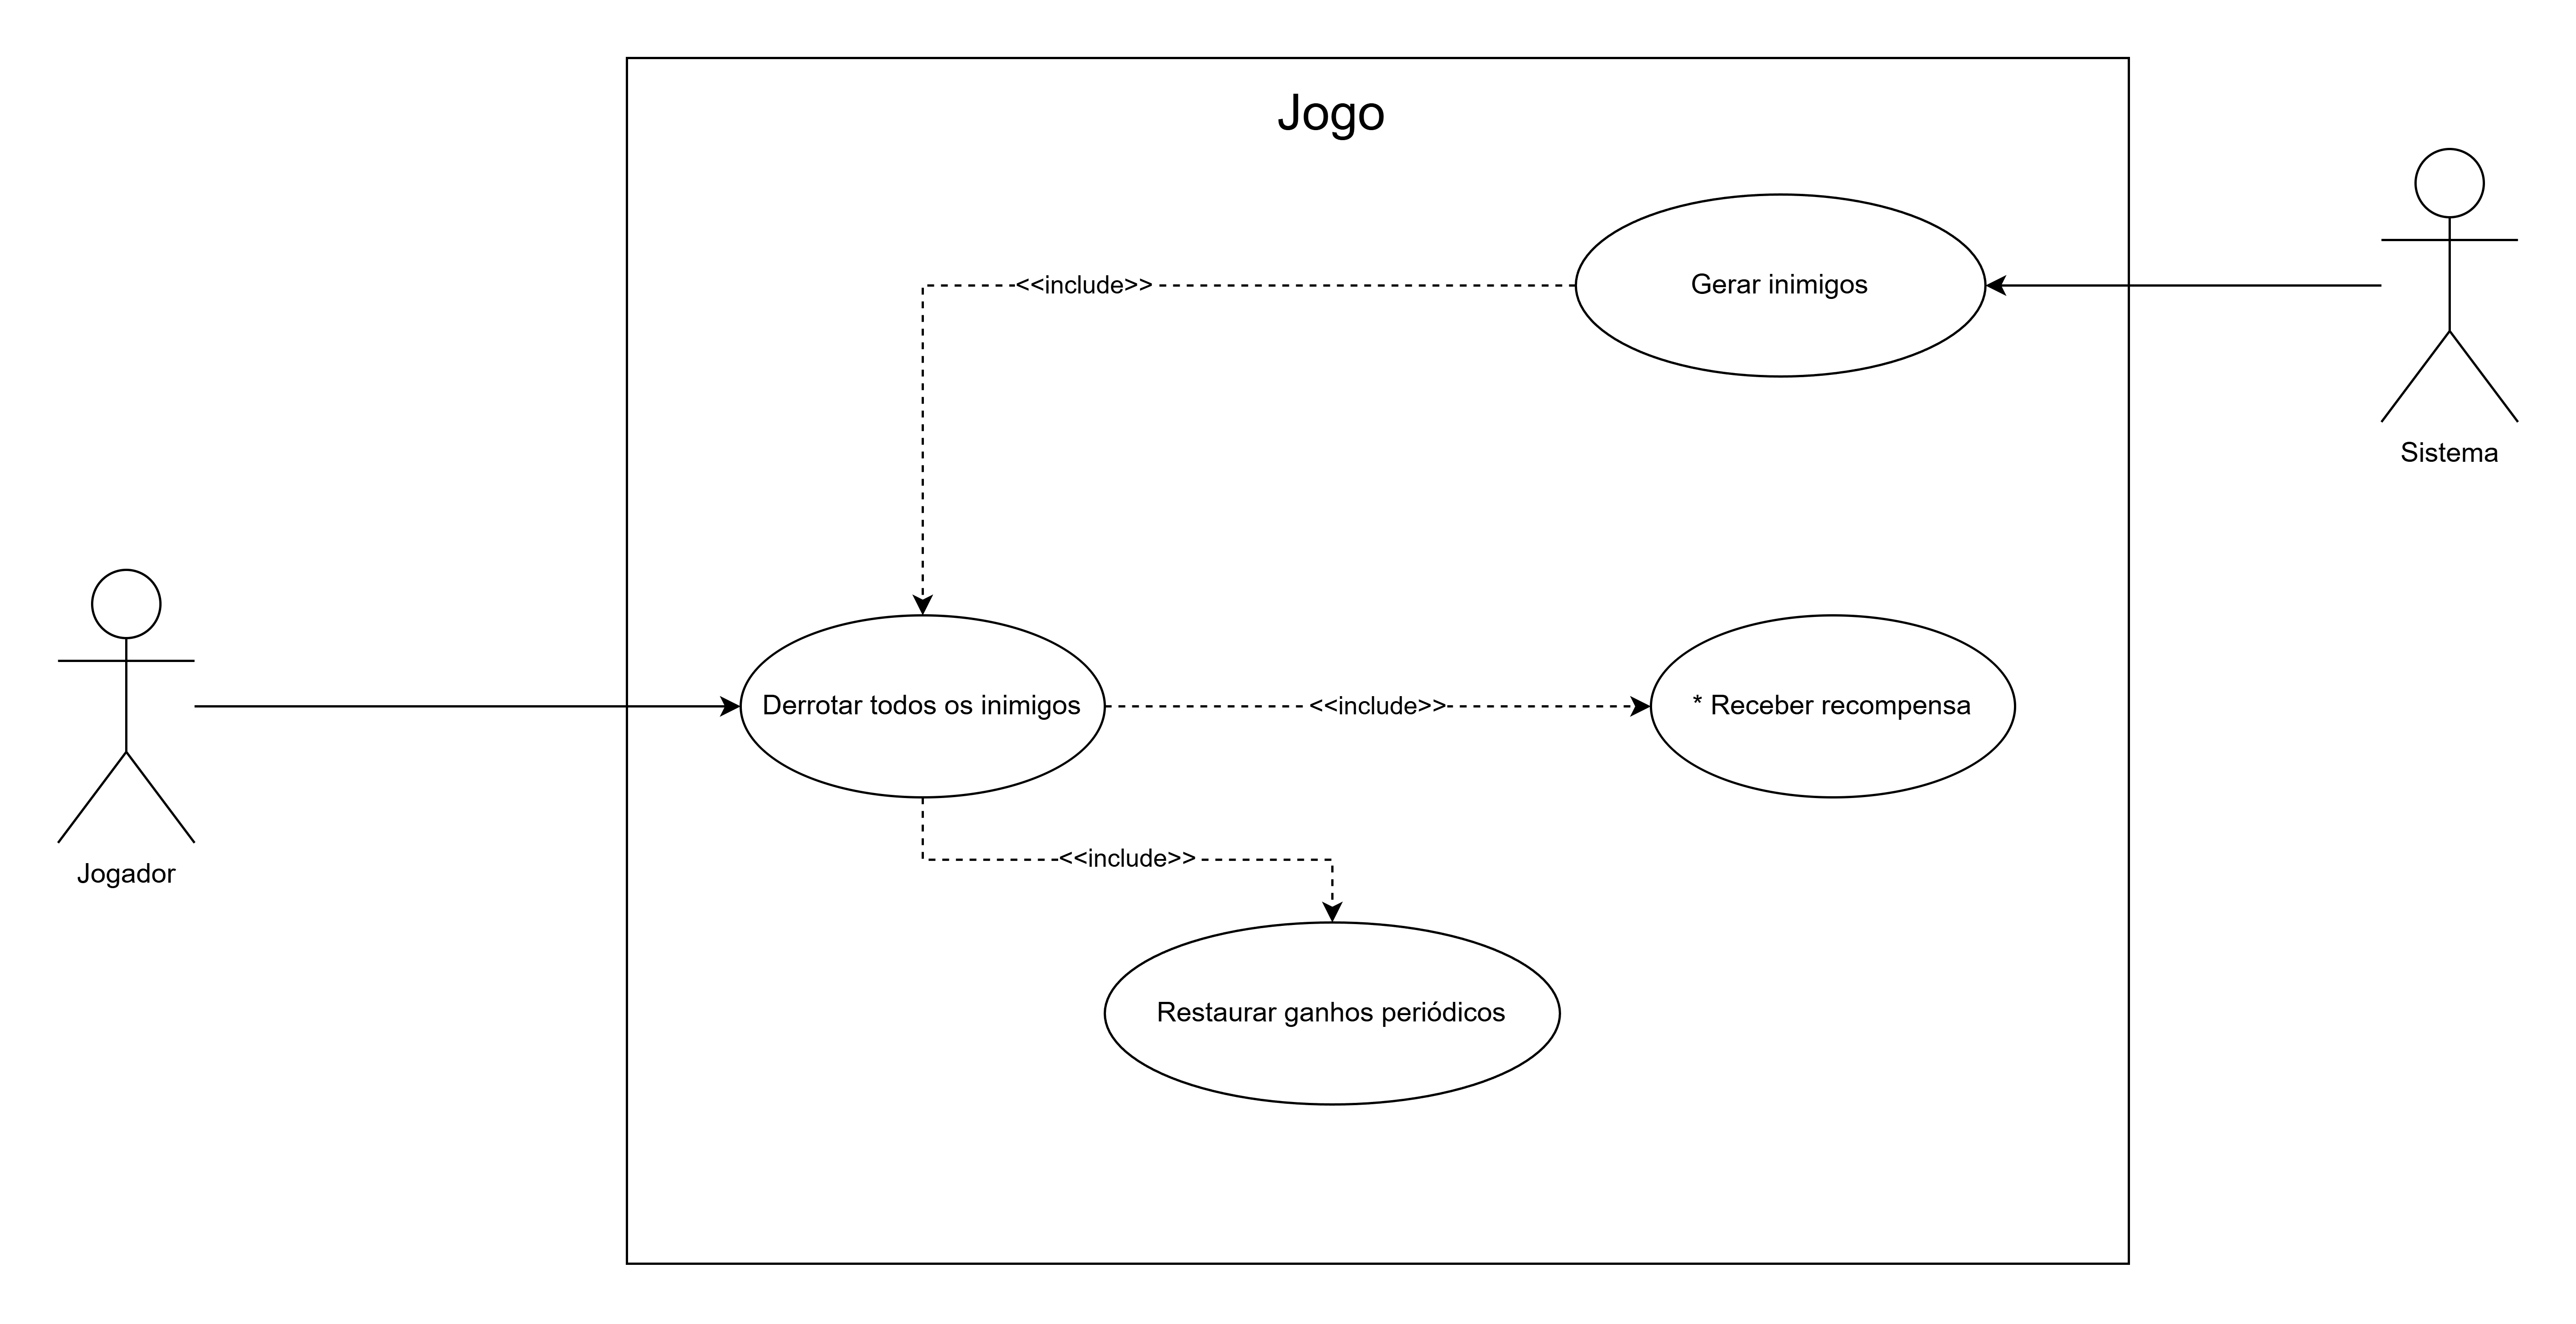
\includegraphics[width=0.9\textwidth]{Diagramas/Use_case_Combate.png}
    \caption{Diagrama de Caso de uso - Combate}
    \label{User_Case_Combat}
\end{figure}

A Figura \ref{User_Case_Combat}, ilustra a interação entre o jogador e o sistema de combate.
Neste sistema, a funcionalidade mais relevante é a "Restaurar ganhos periódicos", uma vez que a partir do momento que o sistema combate "Gera inimigos" os ganhos periódicos são desativados, no entanto,
os custo(prejuízo) não são desativados, o que deixa o jogador numa situação de risco.
O jogador têm de agir rápido para conseguir restaurar os ganhos periódicos, caso contrário, pode perder uma grande quantidade de dinheiro, o que pode levar a uma situação de falência, impossibilitando o pagamento dos custos periódicos, o que leva o jogador a perder o jogo. Esta situação tenta simular o que acontece na relidade, ou seja, quando um data center é atacado pode não conseguir assegurar os seus serviços, resultando em perdas.

\newpage

\section{Implementação}
A implementação constitui a fase em que os planos idealizados são concretizados. 
Nesse sentido, a descrição dos processos será detalhada ao longo desta secção, 
na qual cada subsecção abordará a implementação de uma componente específica 
do projeto.

\subsection{Modelos 3D - Blender}
Dada a natureza do projeto, os modelos 3D assumem um papel de destaque, visto 
que é através destes que o jogador experiencia o mundo e realiza interações. 
Como tal, o seu desenvolvimento deve ser estruturado para maximizar a 
experiência de \textit{gameplay}, mantendo um padrão visual reconhecível e coerente.

Neste sentido, a maioria dos modelos 3D foi desenvolvida por autoria própria, 
recorrendo ao \textit{software} Blender.

\newpage

\subsubsection{Cenário}

\begin{figure}[H]
     \centering
     % Primeira Foto
     \begin{subfigure}[b]{0.3\textwidth}
         \centering
         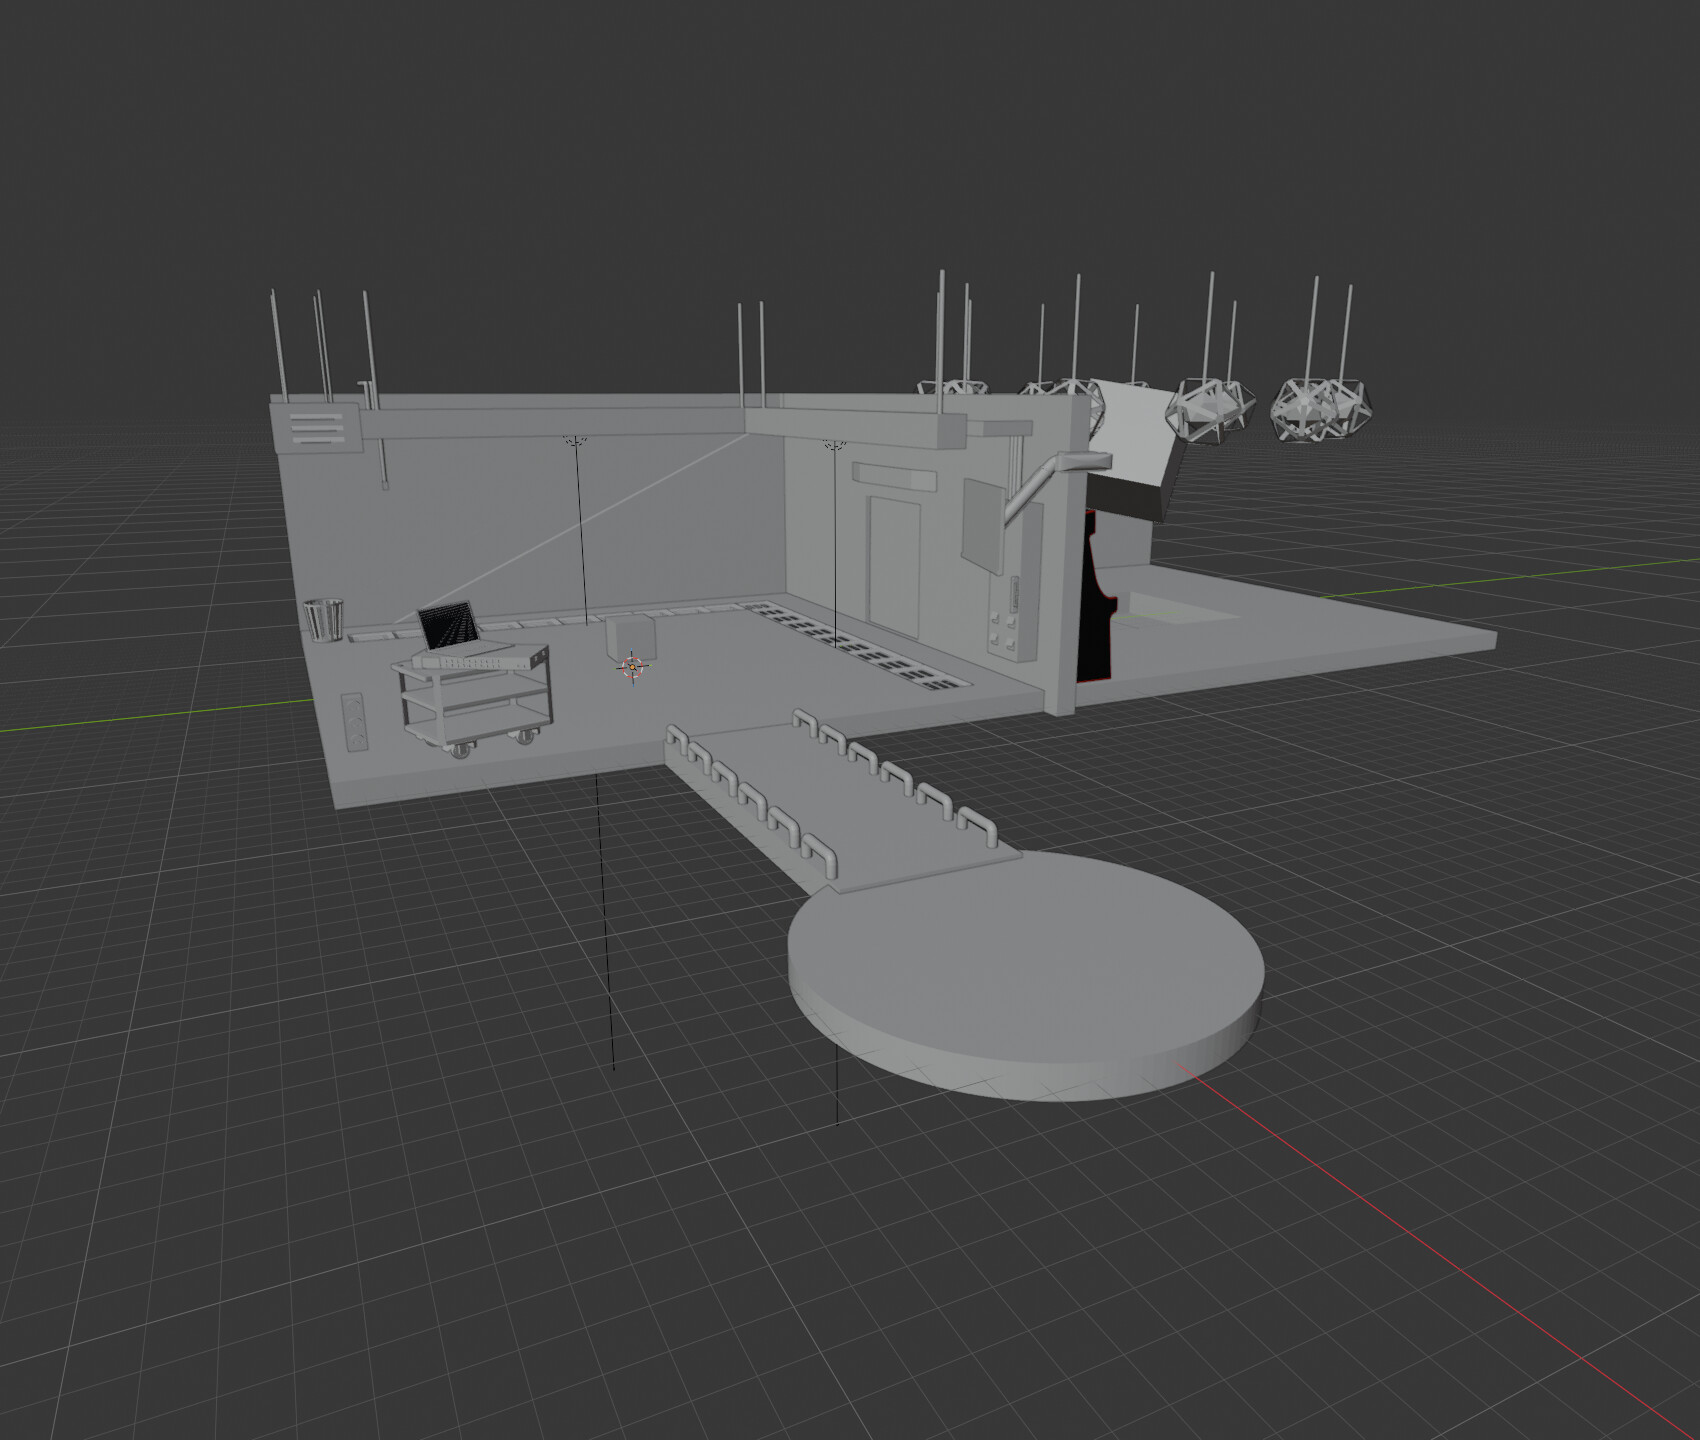
\includegraphics[width=\textwidth]{Blender/CenarioViewPort1.jpg}
         \caption{Cenário Vista de \textit{ViewPort} 1}
         \label{fig:foto1}
     \end{subfigure}
     \hfill
     % Segunda Foto
     \begin{subfigure}[b]{0.3\textwidth}
         \centering
         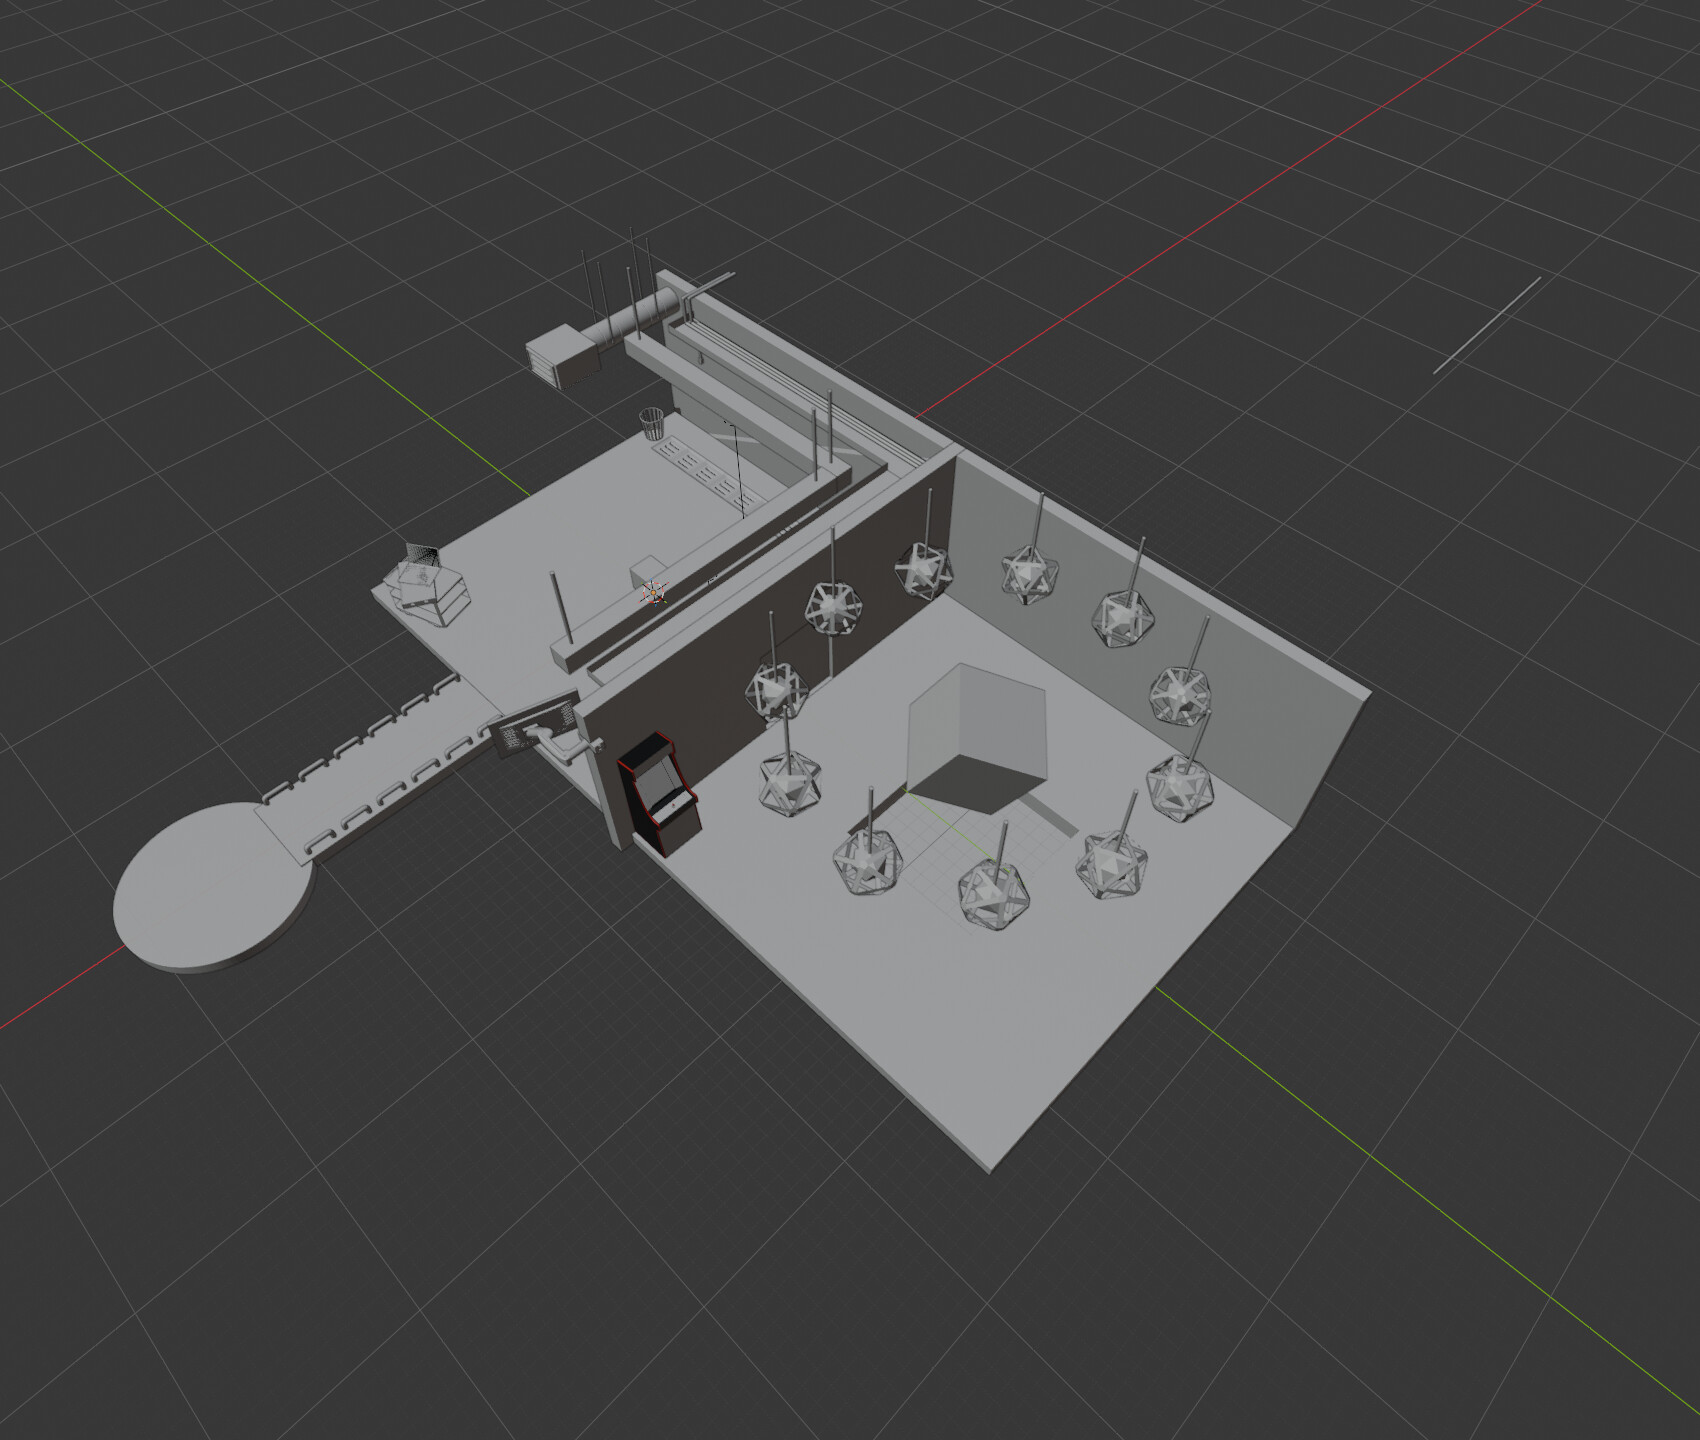
\includegraphics[width=\textwidth]{Blender/CenarioViewPort2.jpg}
         \caption{Cenário Vista de \textit{ViewPort} 2}
         \label{fig:foto2}
     \end{subfigure}
     \hfill
     % Terceira Foto
     \begin{subfigure}[b]{0.3\textwidth}
         \centering
         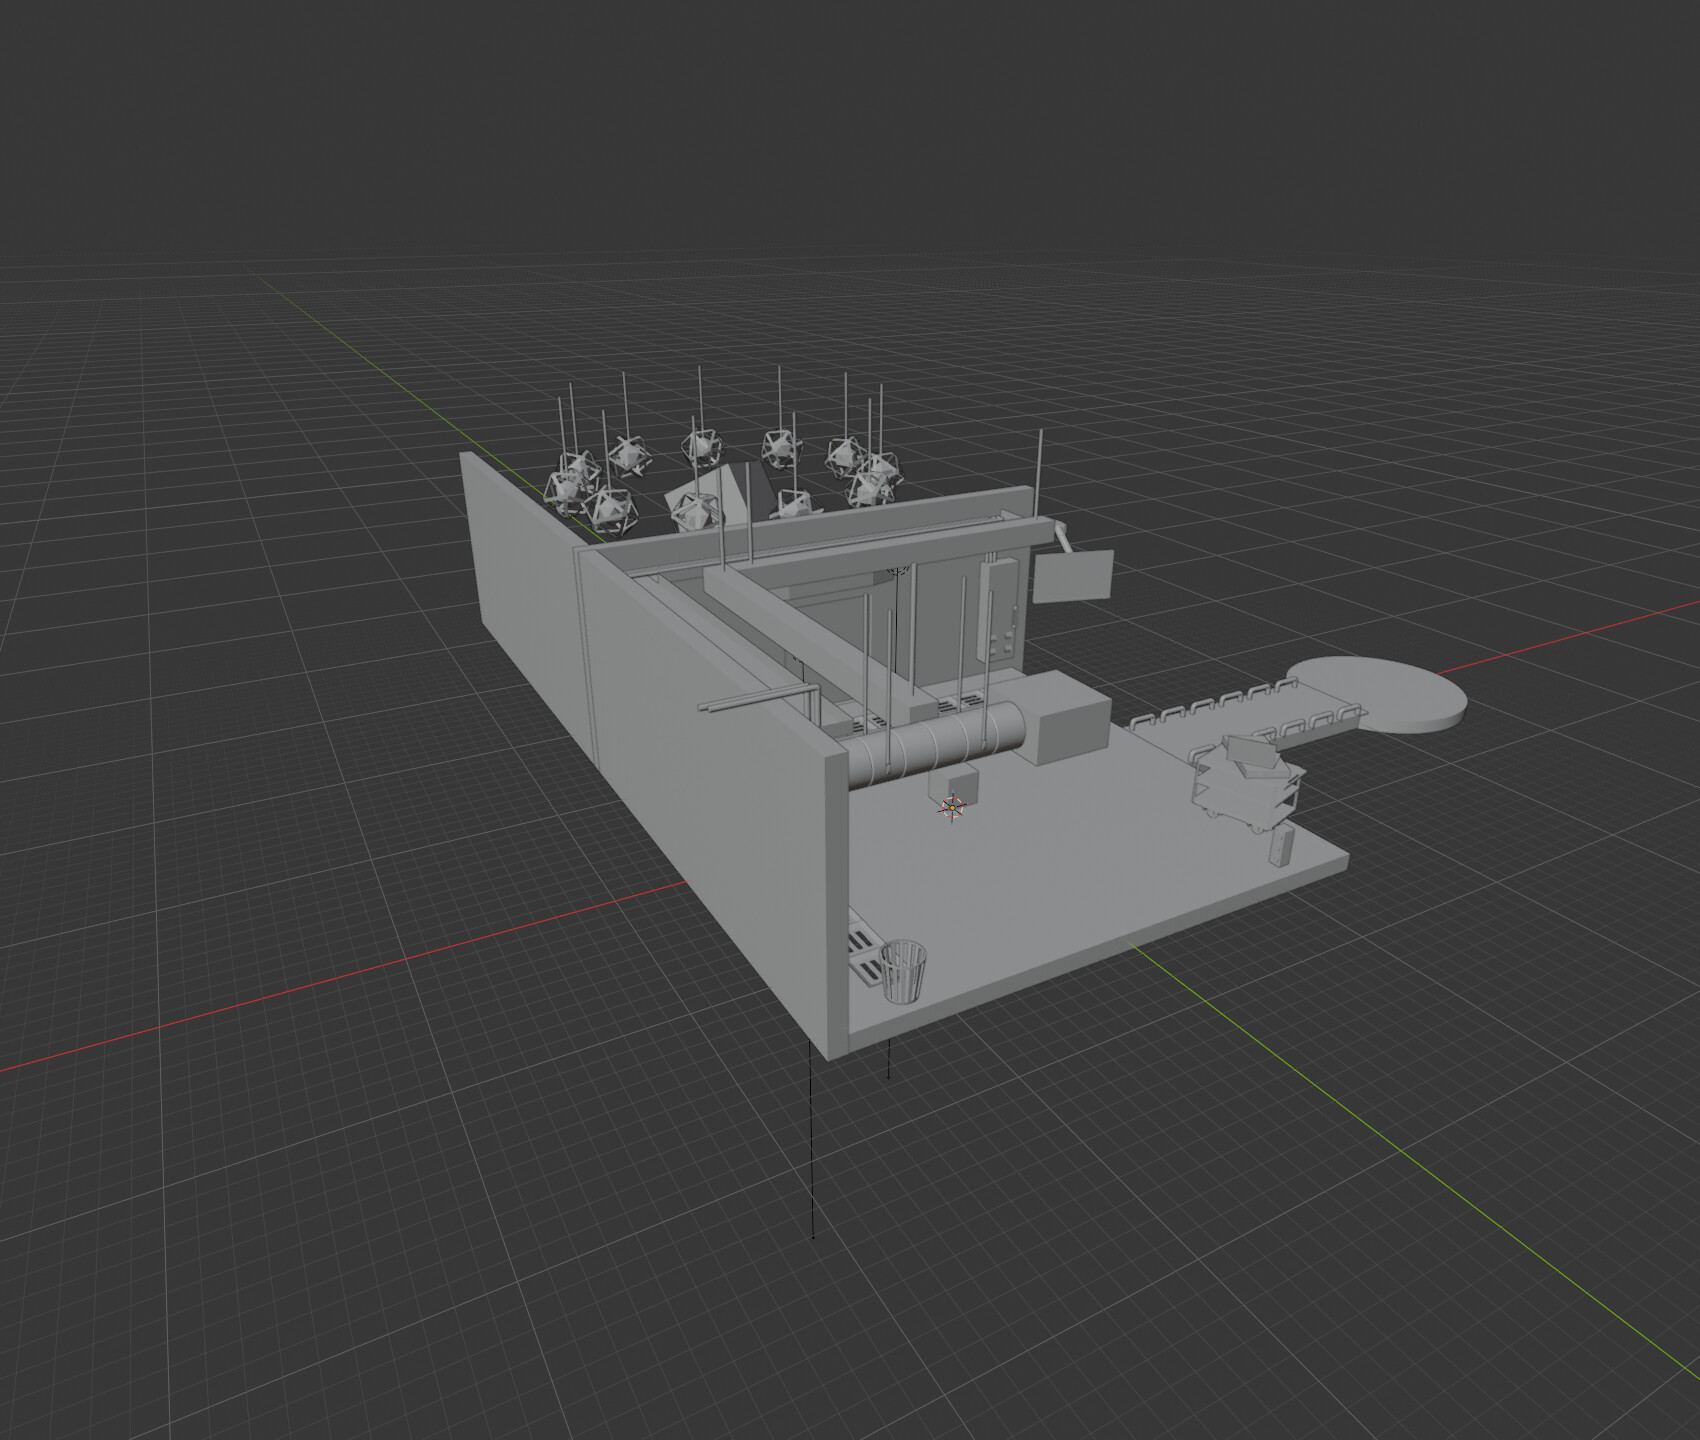
\includegraphics[width=\textwidth]{Blender/CenarioViewPort3.jpg}
         \caption{Cenário Vista de \textit{ViewPort} 3}
         \label{fig:foto3}
     \end{subfigure}
     
     \caption{Vistas de \textit{ViewPort} do cenário.}
     \label{CenarioViewportGroup3.1}
\end{figure}

\begin{figure}[H]
    \centering
    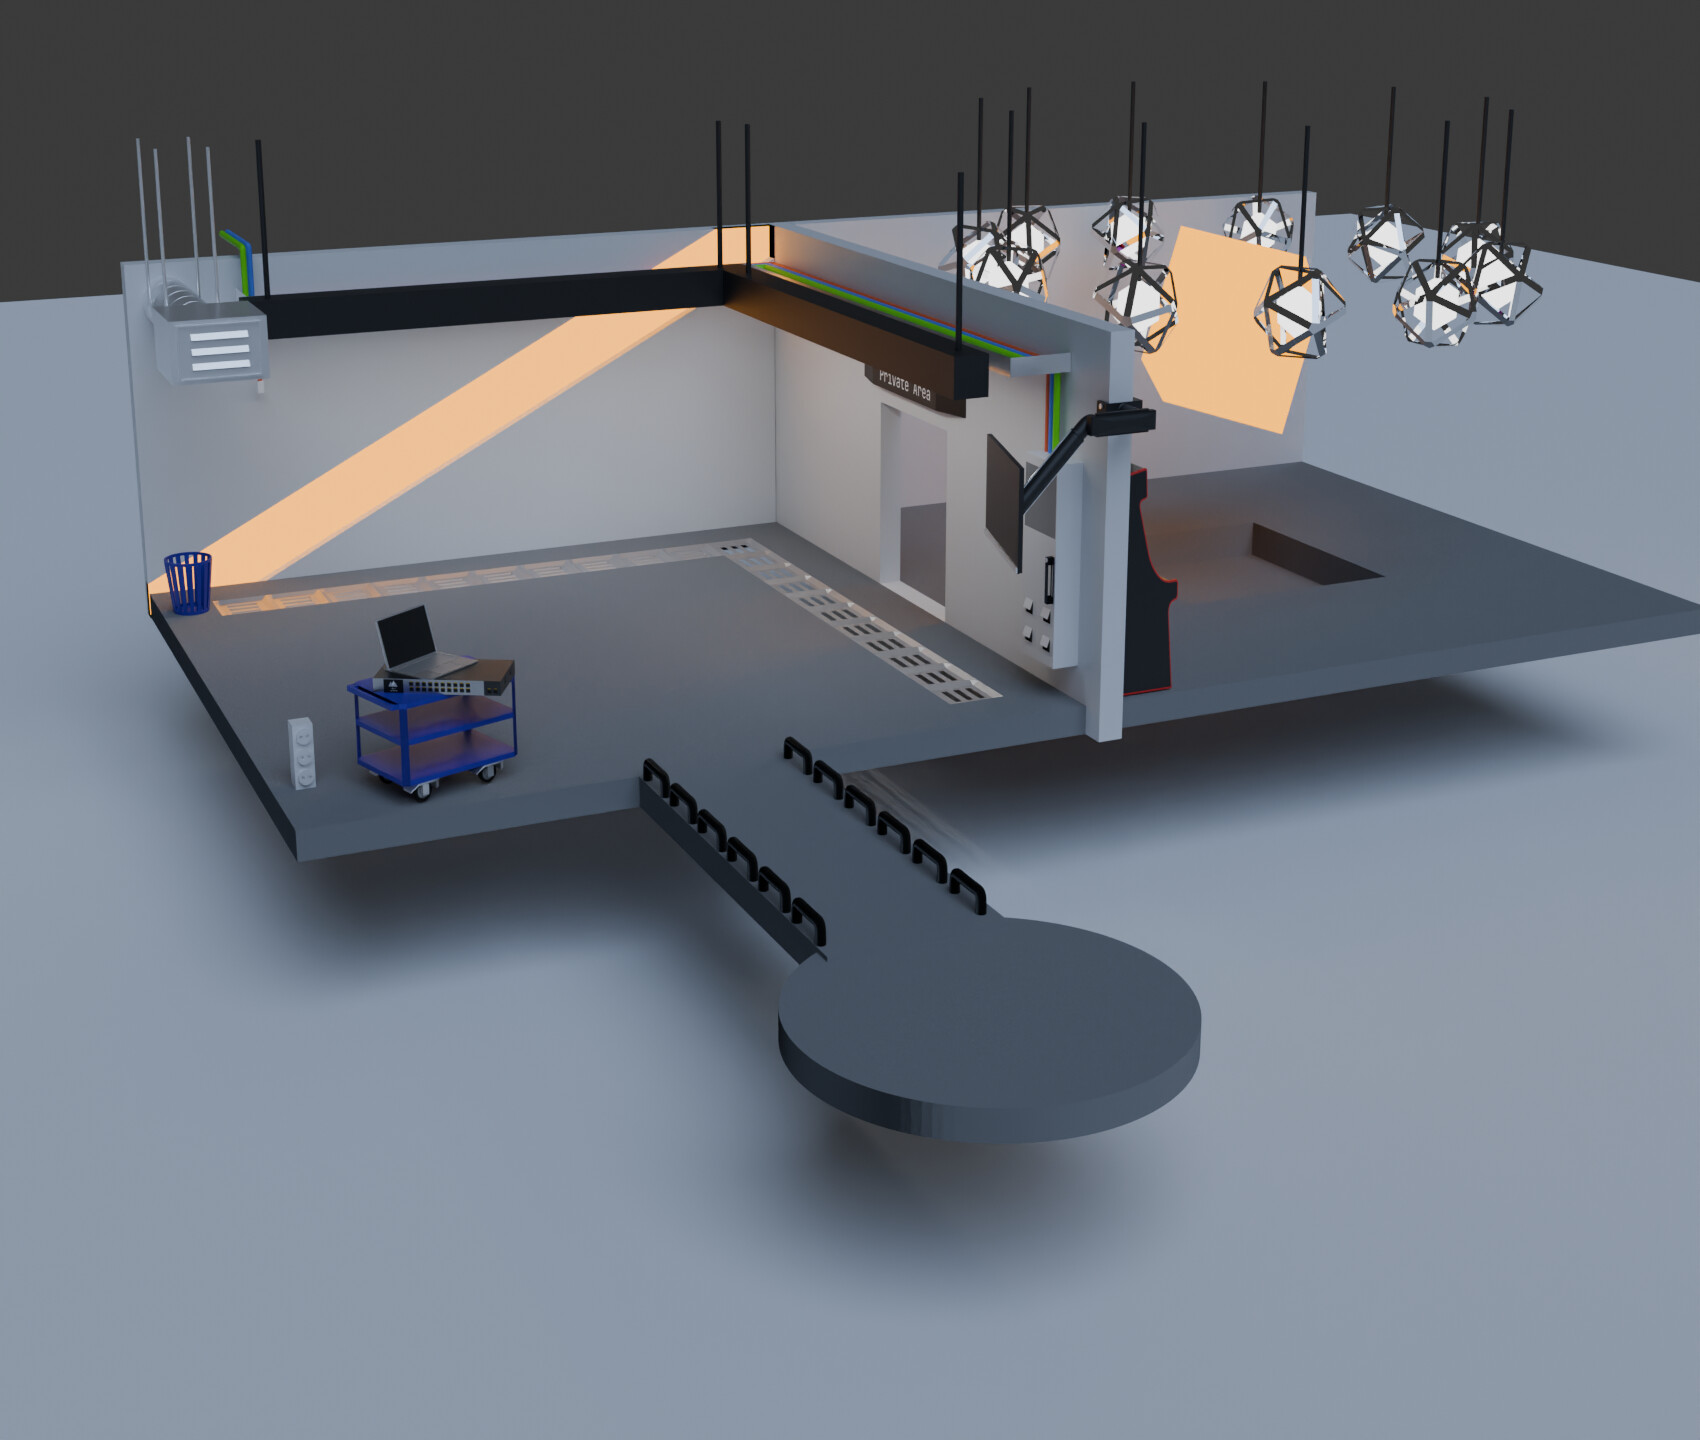
\includegraphics[width=0.65\textwidth]{Blender/CenárioRender.jpg}
    \caption{Vista renderizada do cenário do jogo.}
    \label{CenarioRender1}
\end{figure}

As Figuras \ref{CenarioViewportGroup3.1} e \ref{CenarioRender1}
ilustra o trabalho desenvolvido para o cenário.
Todos os subcomponentes dos cenários, tais como, mesas, computadores, e outros detalhes
desenvolvidos com a ajuda do \textit{software}.

\newpage

\subsubsection{Canhão}
\label{Sec:Canhão}

\begin{figure}[H]
     \centering
     % Primeira Foto
     \begin{subfigure}[b]{0.3\textwidth}
         \centering
         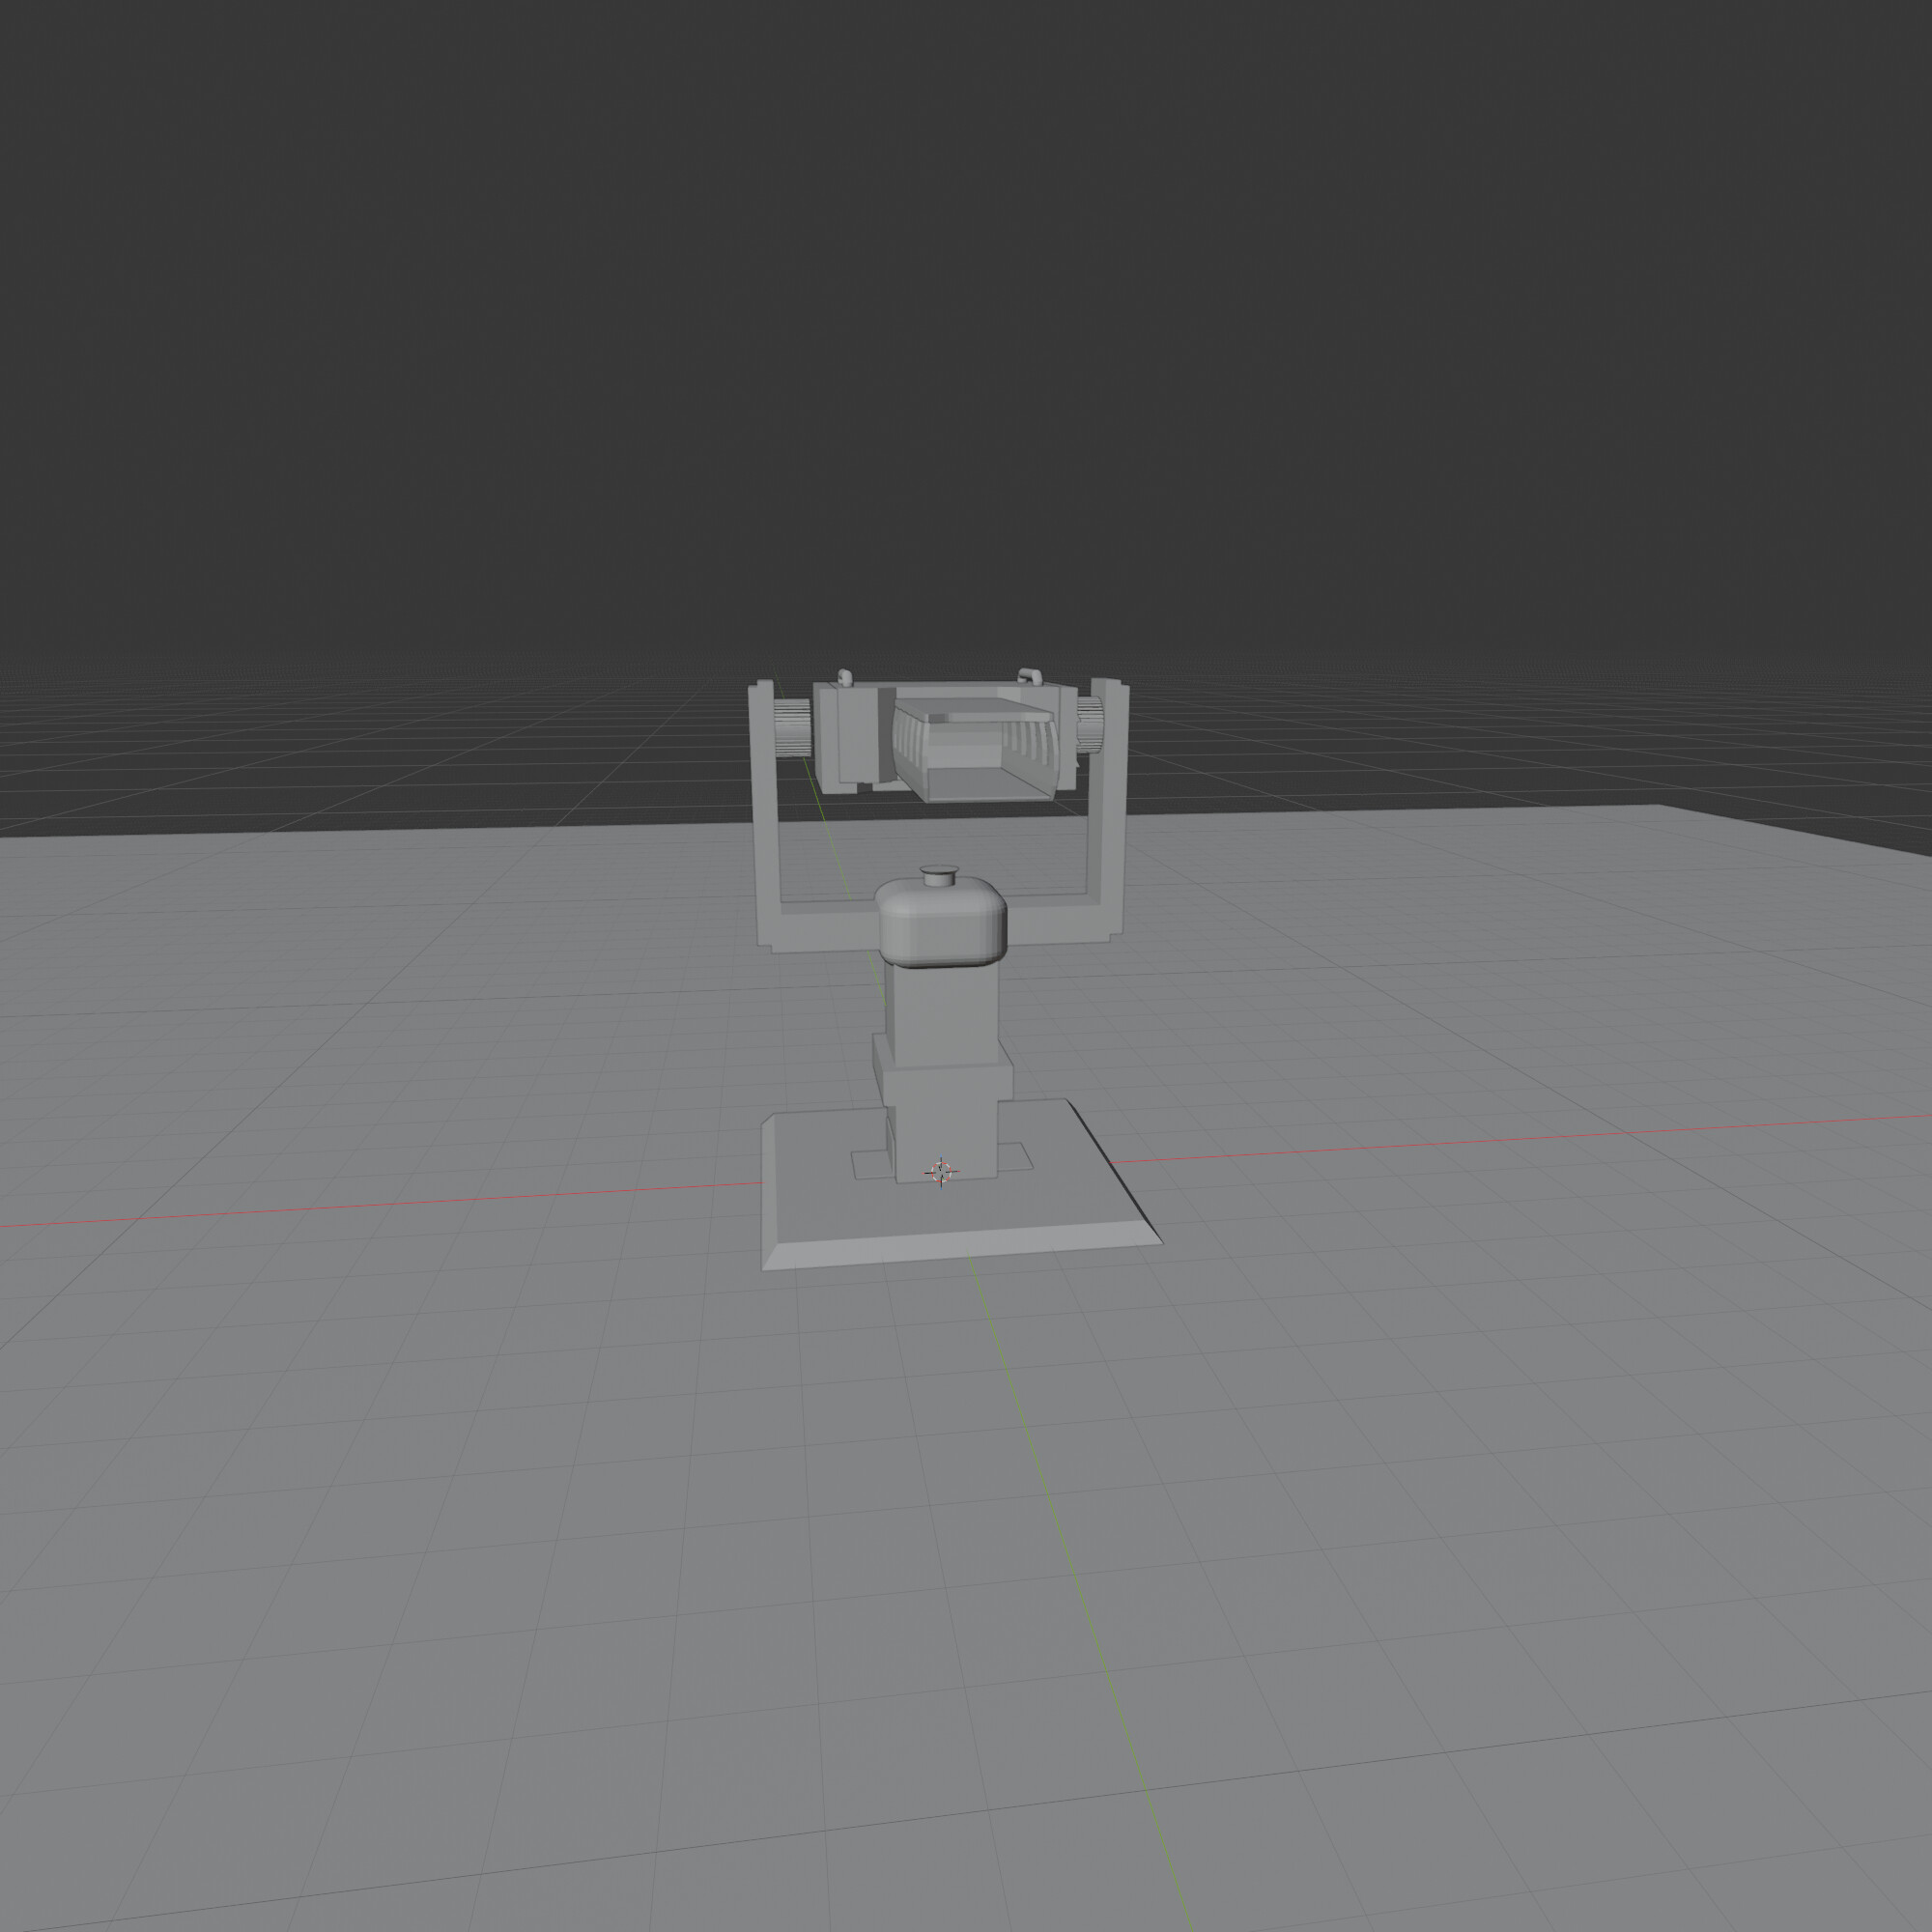
\includegraphics[width=\textwidth]{Blender/CanhaoViewPort1.jpg}
         \caption{Cenário Vista de \textit{ViewPort} 1}
         \label{fig:foto1Canhao}
     \end{subfigure}
     \hfill
     % Segunda Foto
     \begin{subfigure}[b]{0.3\textwidth}
         \centering
         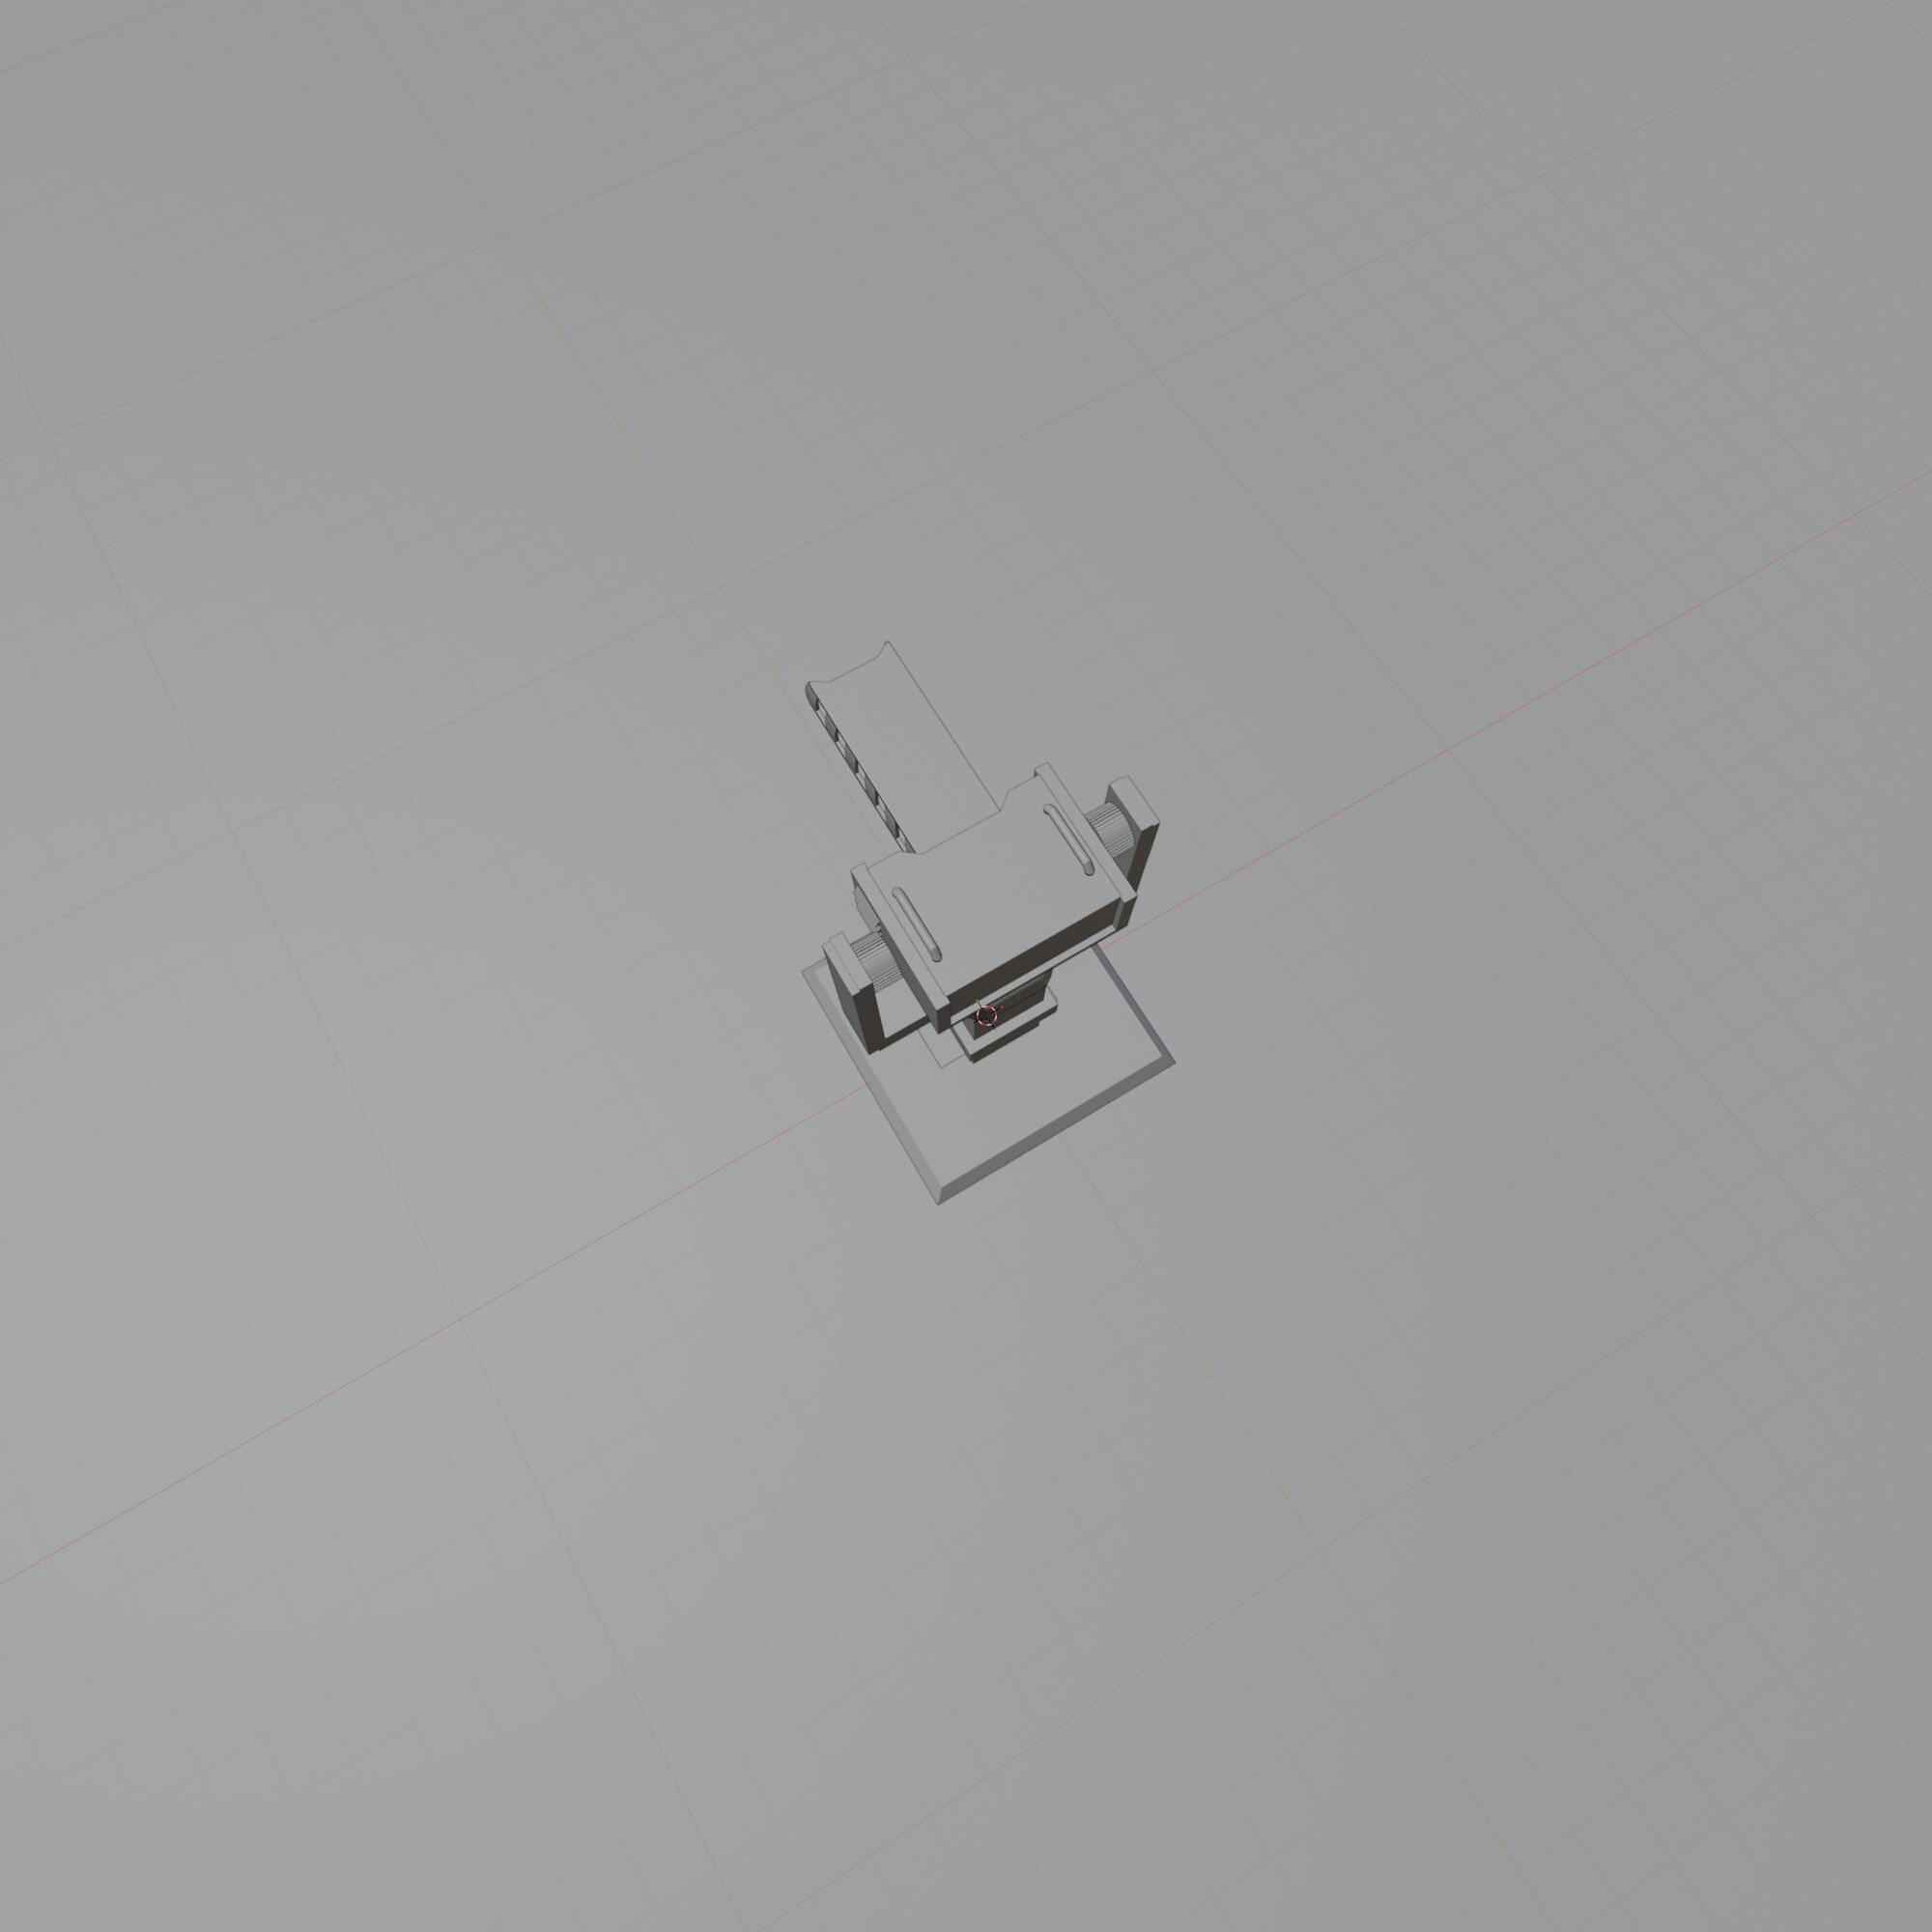
\includegraphics[width=\textwidth]{Blender/CanhaoViewPort2.jpg}
         \caption{Cenário Vista de \textit{ViewPort} 2}
         \label{fig:foto2Canhao}
     \end{subfigure}
     \hfill
     % Terceira Foto
     \begin{subfigure}[b]{0.3\textwidth}
         \centering
         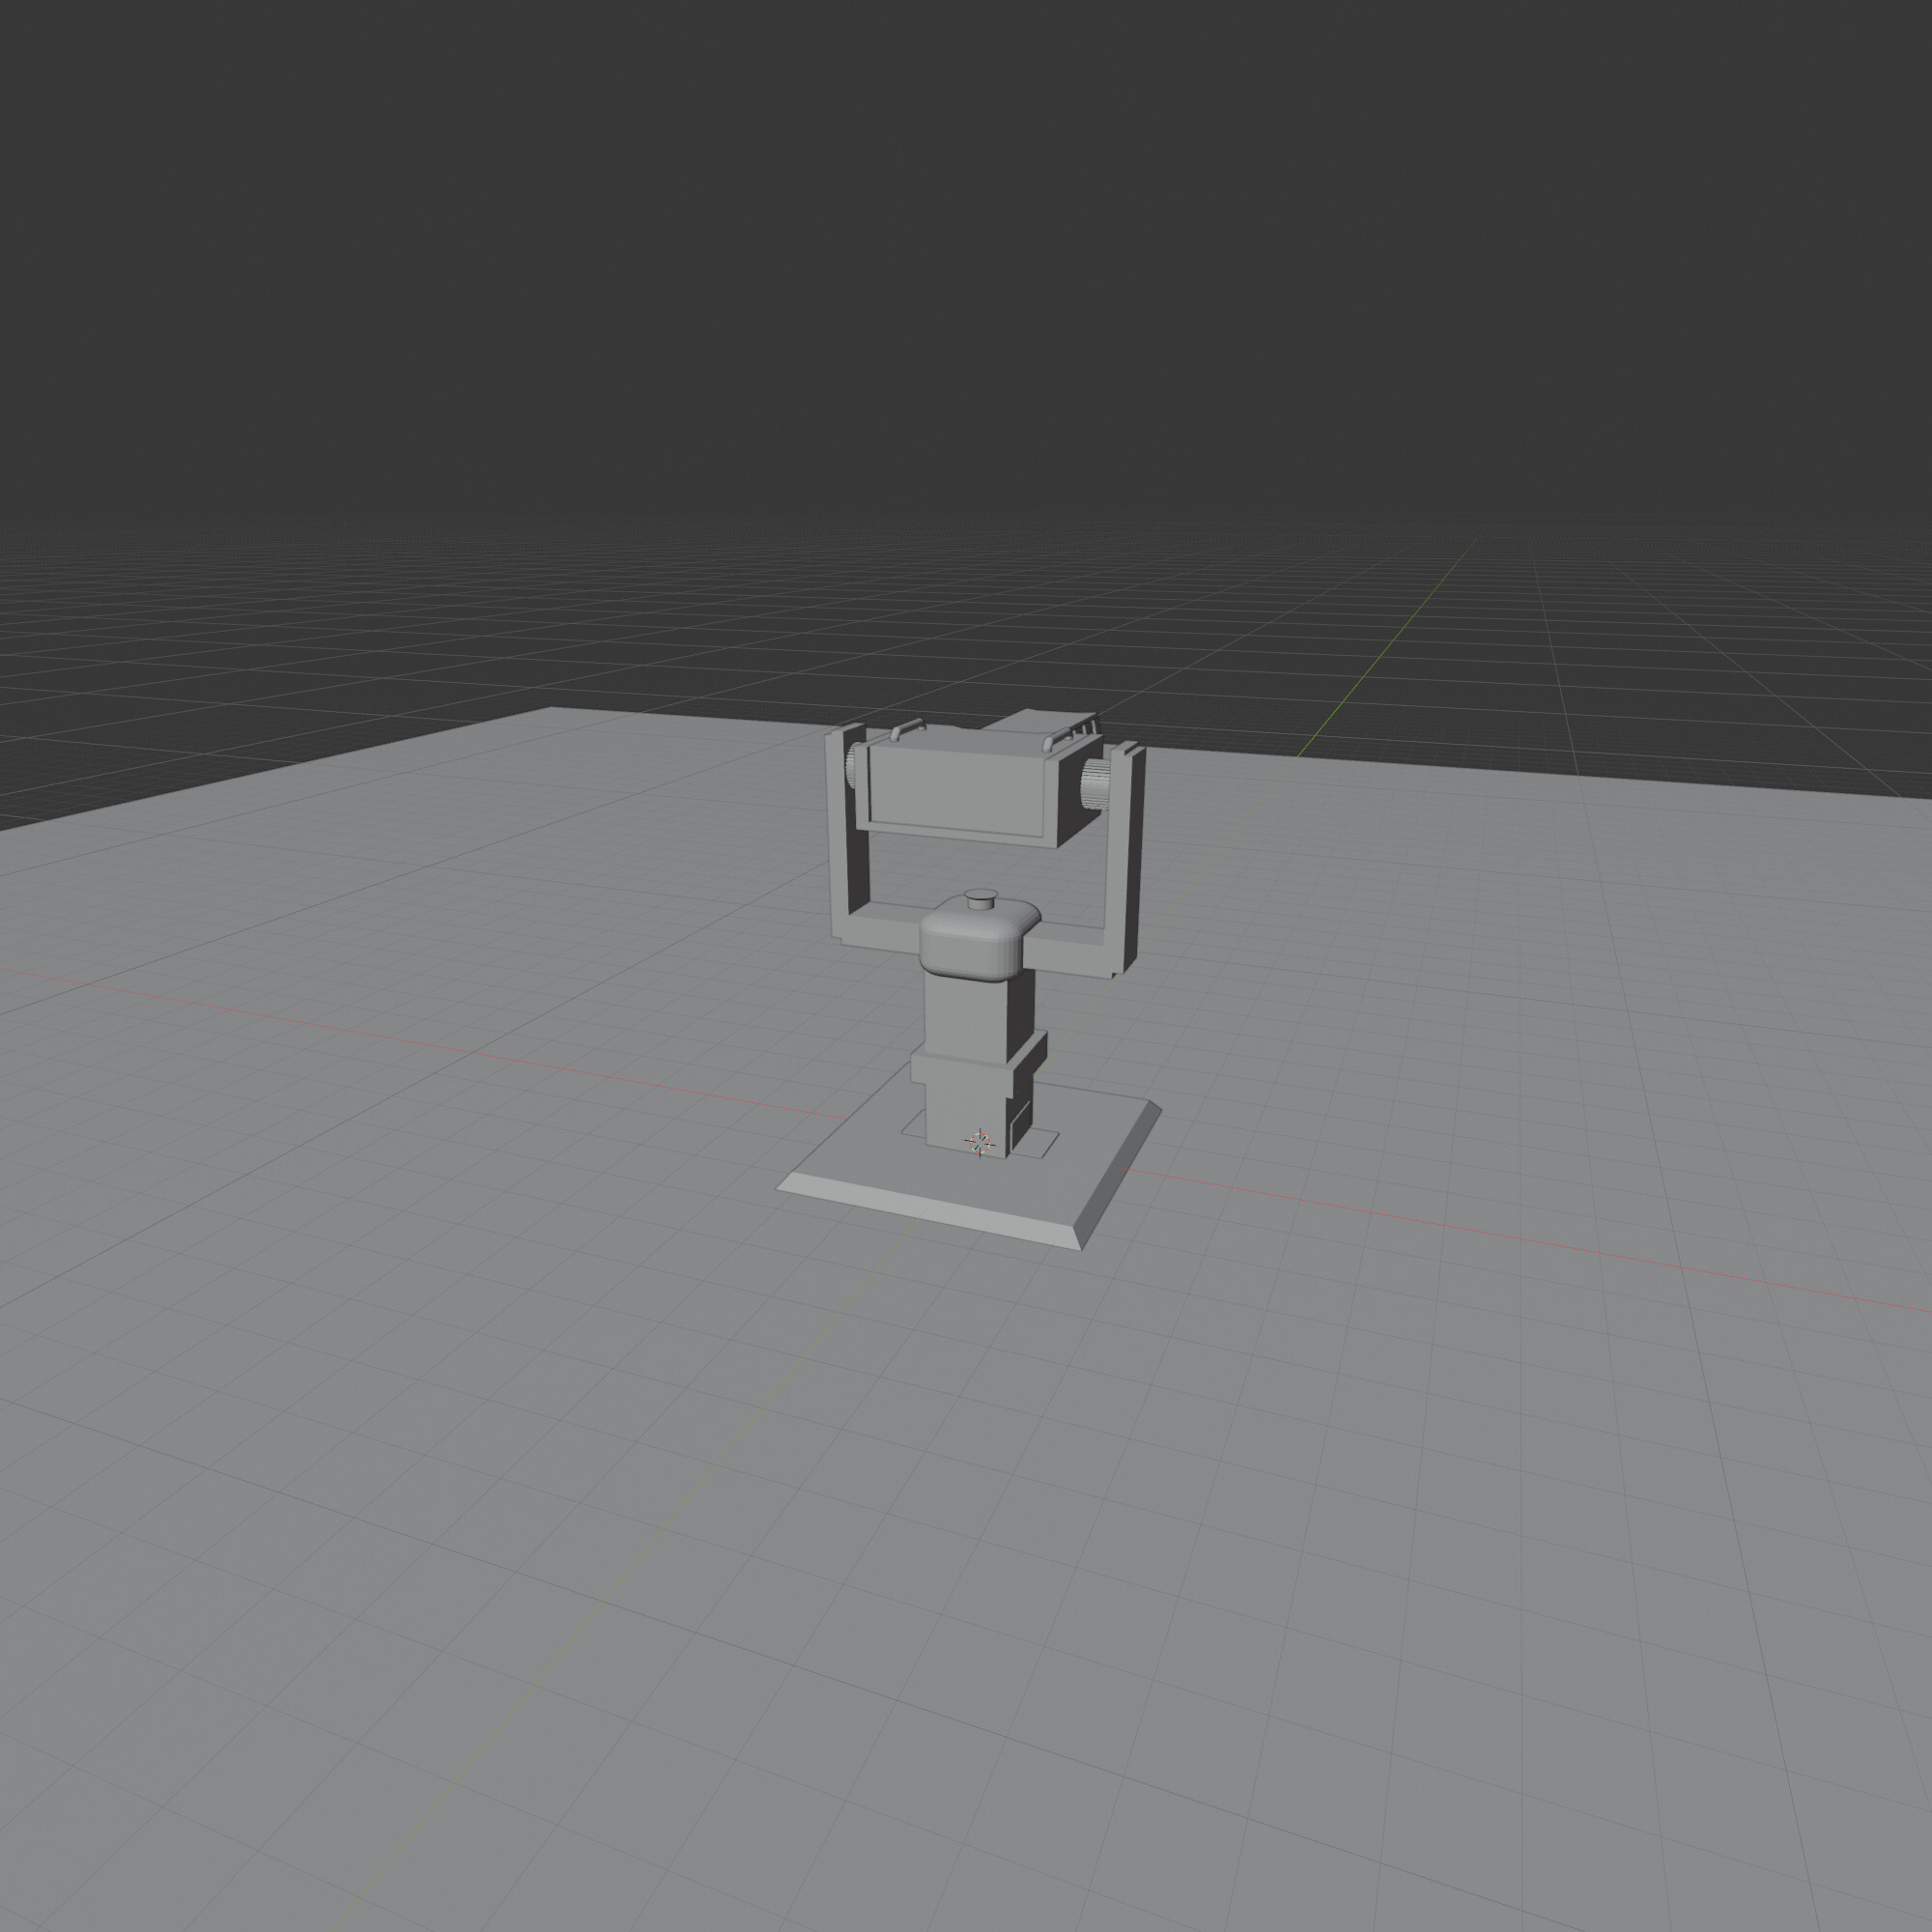
\includegraphics[width=\textwidth]{Blender/CanhaoViewPort3.jpg}
         \caption{Cenário Vista de \textit{ViewPort} 3}
         \label{fig:foto3Canhao}
     \end{subfigure}
     
     \caption{Vistas de \textit{ViewPort} do canhão.}
     \label{CanhaoViewportGroup3.1}
\end{figure}

\begin{figure}[H]
    \centering
    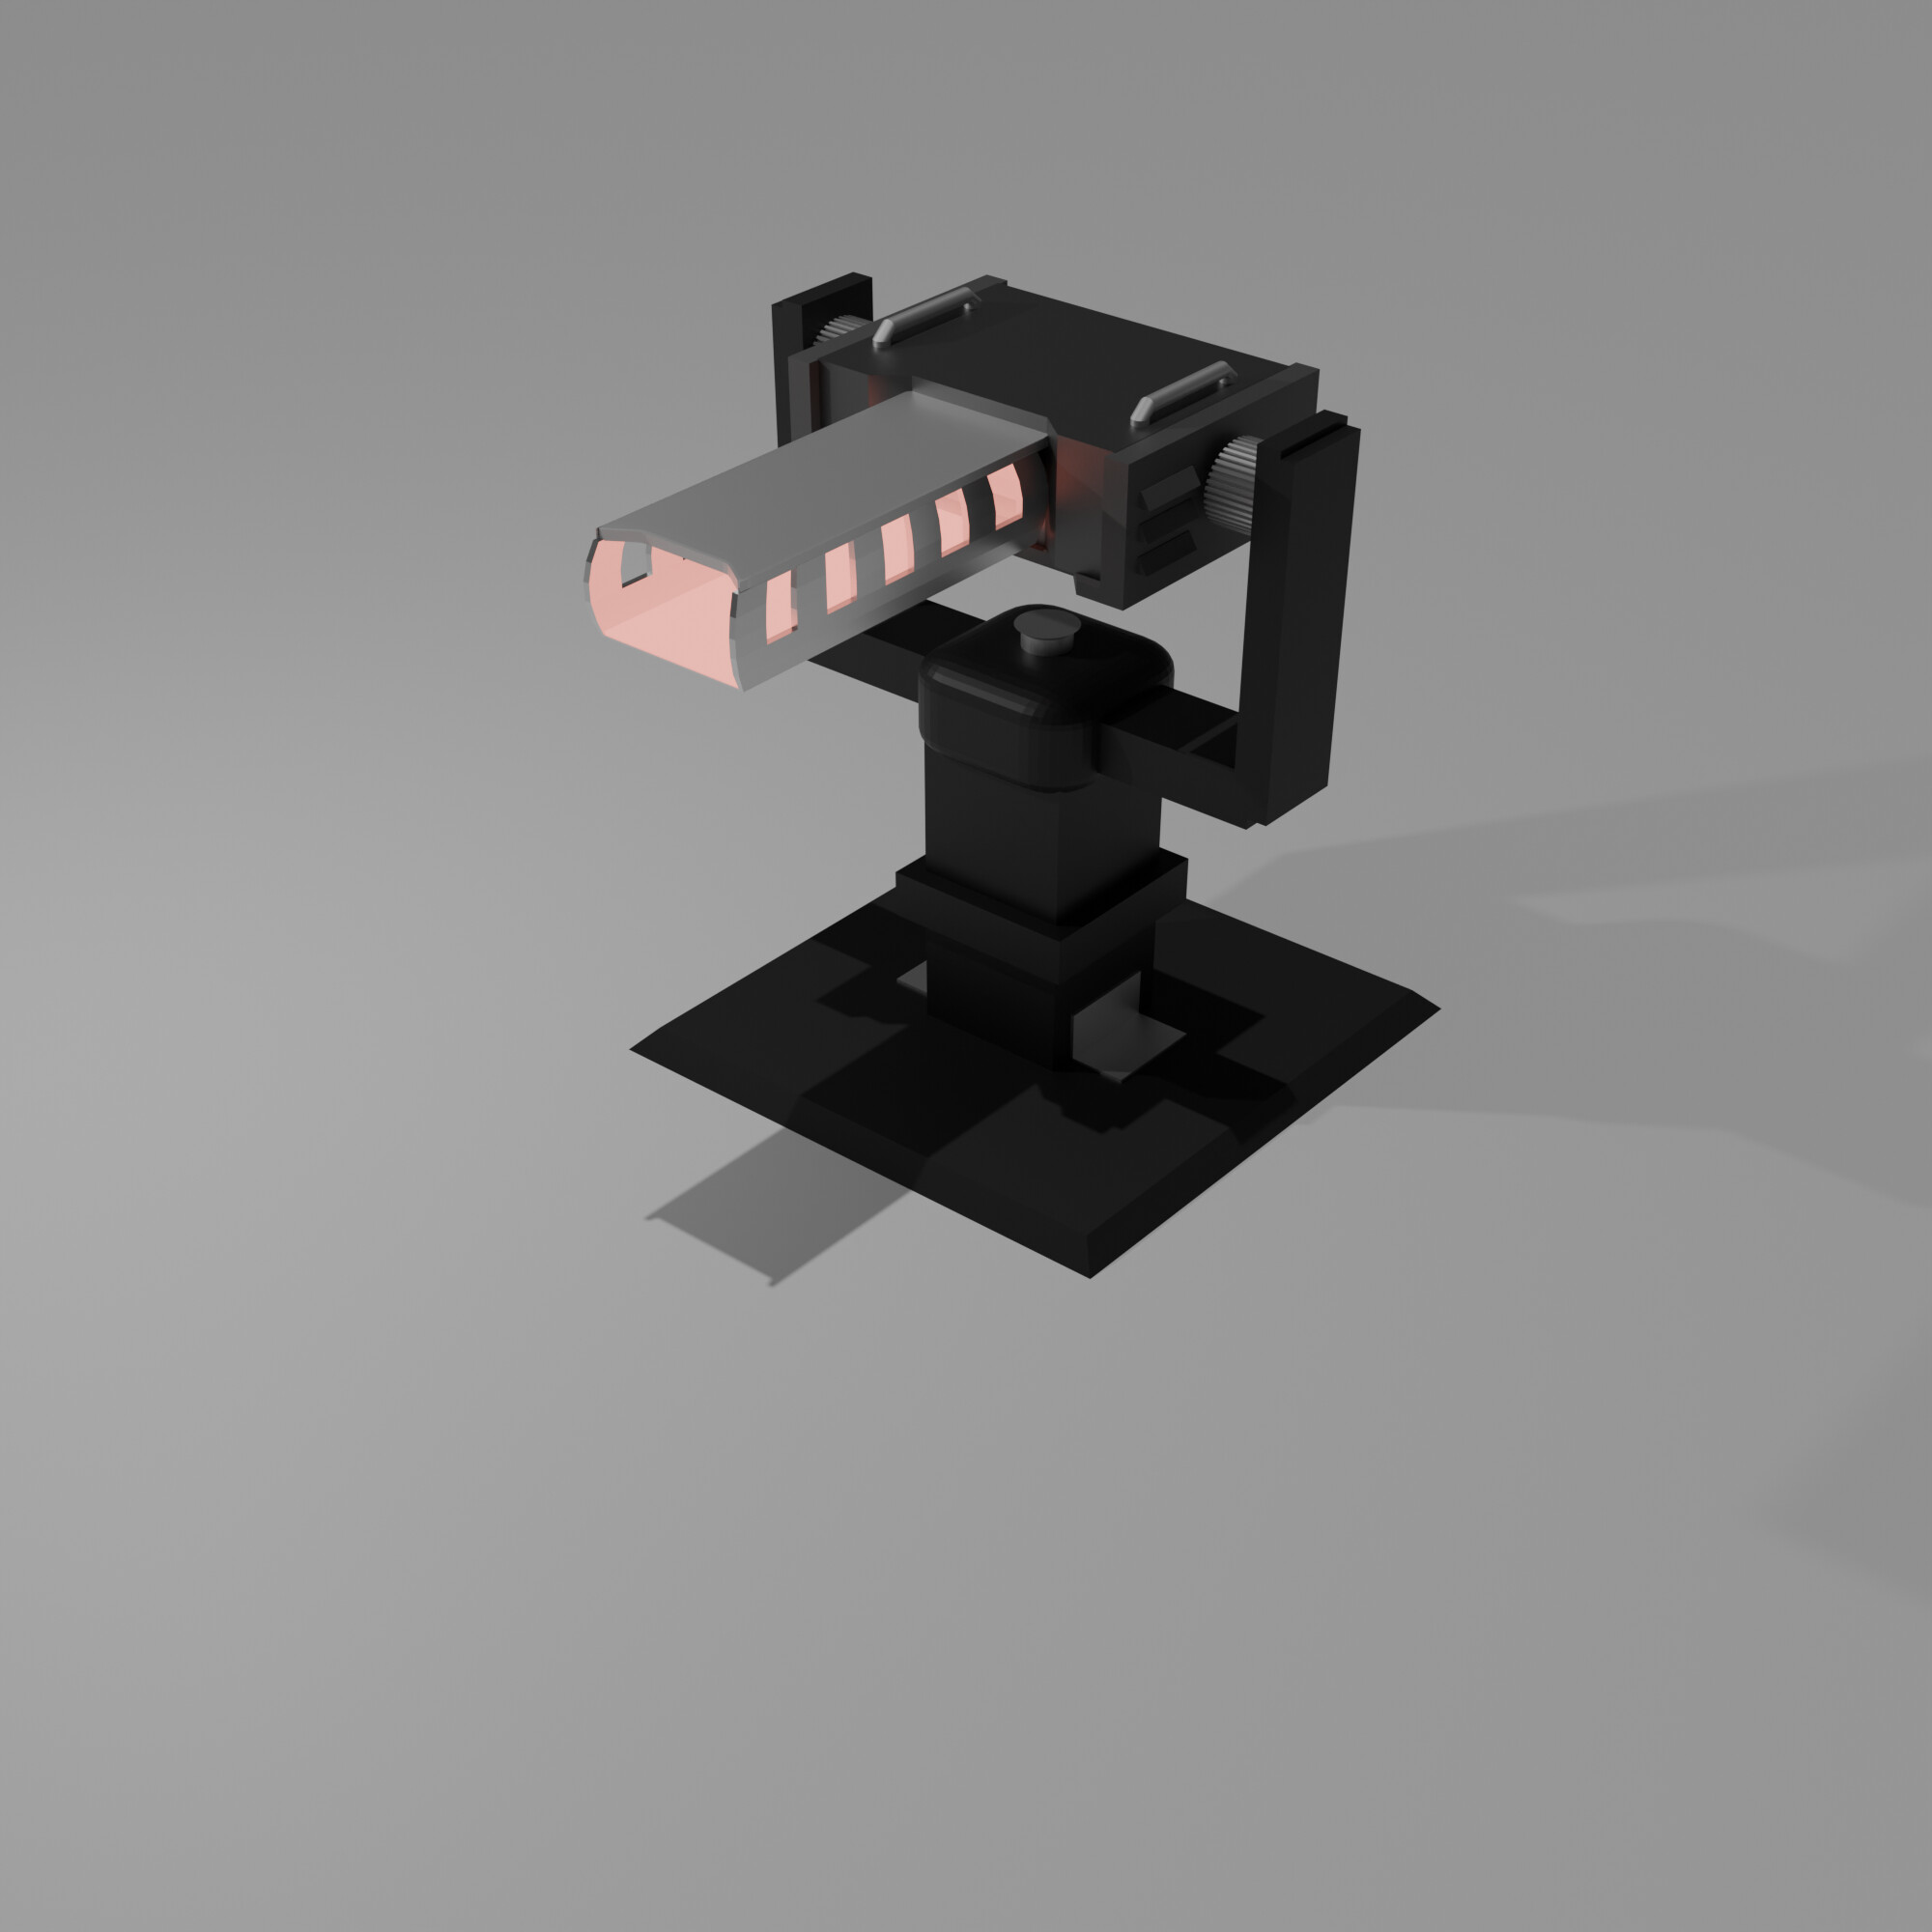
\includegraphics[width=0.55\textwidth]{Blender/CanhaoRender.jpg}
    \caption{Vista renderizada do canhão.}
    \label{CanhaoRender1}
\end{figure}

As Figuras \ref{CanhaoViewportGroup3.1} e \ref{CanhaoRender1} ilustram
o modelo do canhão. Os processos de modelação assim como de pintura 
de materiais, foram desenvolvidos dentro do \textit{software} Blender.

Com o design deste modelo, pretenda-se transmitir uma sensação de 
futurismo moderada, 
mas que, ao mesmo tempo, harmozine com o cenário restante.

\subsection{Imagens e \textit{assets} 2D}

Embora não sejam tão utilizados quanto os ativos 3D, os ativos 
2D apresentam um papel bastante importante, sobretudo para elementos
de \ac{UI} e para a idealização do contexto de elementos.

\subsubsection{Idealização do personagem}

\begin{figure}[H]
    \centering
    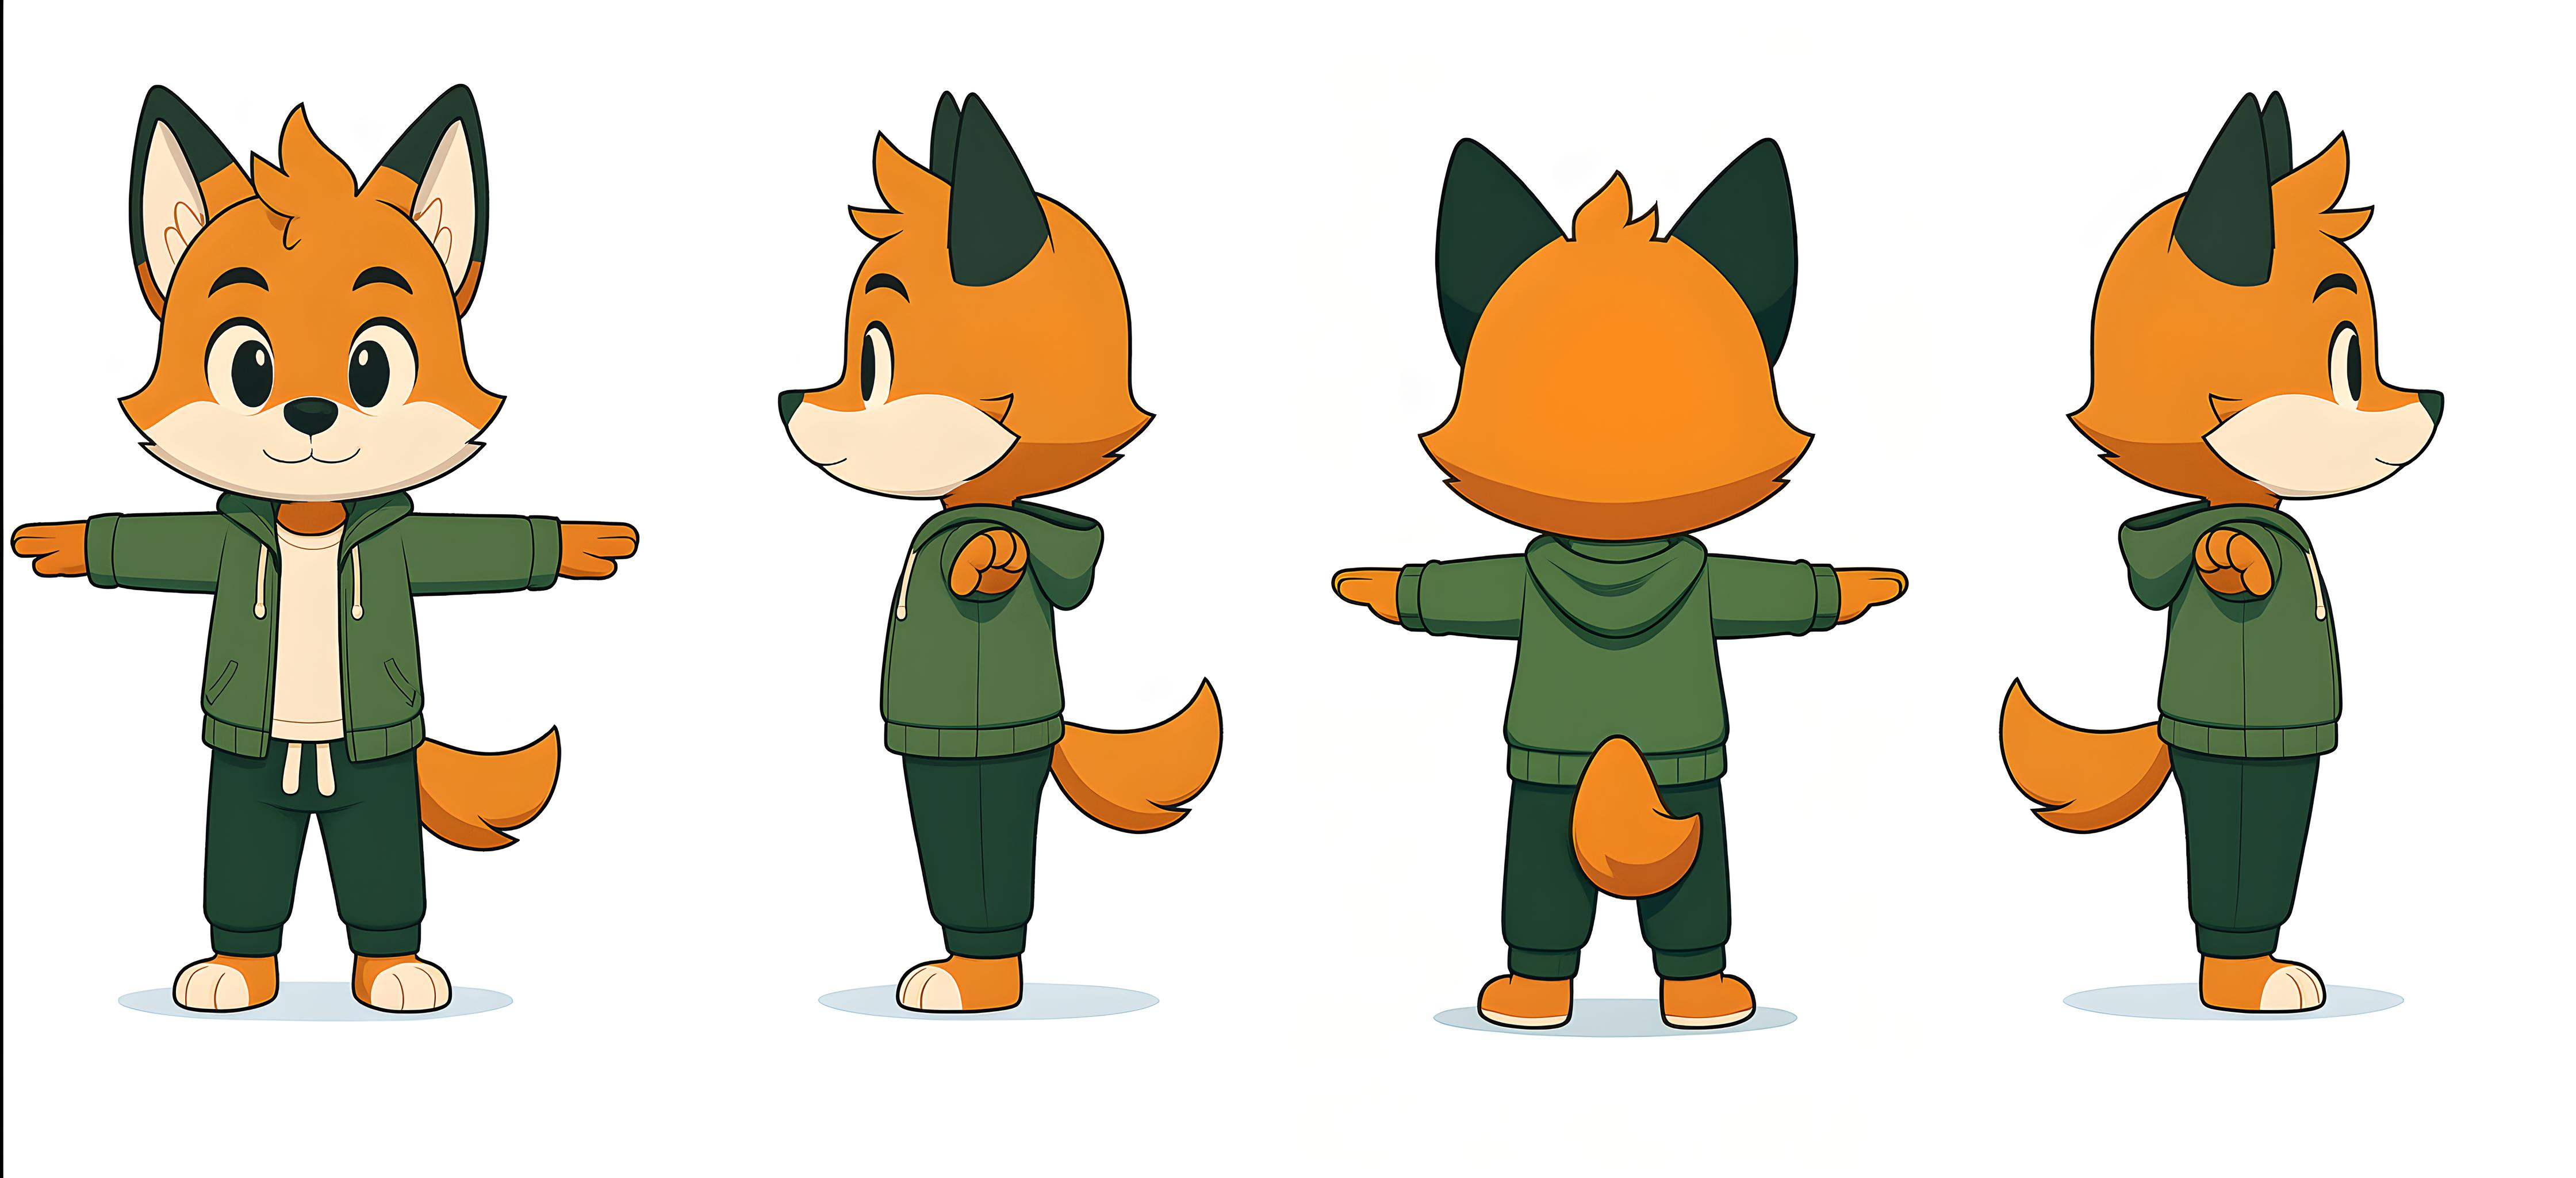
\includegraphics[width=0.8\textwidth]{images/Character_image.jpg}
    \caption{Ilustração do personagem feita com o uso da \ac{IA} - Nano Banana (Gemini)}
    \label{idealizacaoCharacter}
\end{figure}

Durante o processo criativo do personagem, utilizou-se a ferramenta 
Nano Banana do Gemini para gerar a Figura \ref{idealizacaoCharacter}. 
O objetivo foi representar visualmente as suas características físicas, 
de maneira que, esta possa ser utilizada por outras ferramentas de IA, 
tais como o Chat 3D, para a criação de um modelo tridimensional.

\subsubsection{\textit{Frames} para a criação de animações 2D}

No contexto de jogos de vídeo, transmitir \textit{feedbacks} ao jogador
é um dos processos mais importantes, uma vez que eles funcionam como uma
confirmação que uma ação foi realizada e/ou ajudam a construir a experiência
facilitando a evocação de emoções para jogador.

\textit{Feedbacks} podem ser transmitidos, através de \ac{VFX}, animações e efeitos sonoros,
por exemplo, efeitos visuais de faíscas no disparo de uma arma, até animações
do personagem a andar, etc\dots

Posto isto, para a construção de certos \textit{feedbacks} visuais, foram criados \textit{frames} 2D, utilizando o \textit{framework} Processing, os quais foram posteriormente utilizados para a construção de animações 2D dentro da Unity.

\begin{figure}[H]
    \centering
    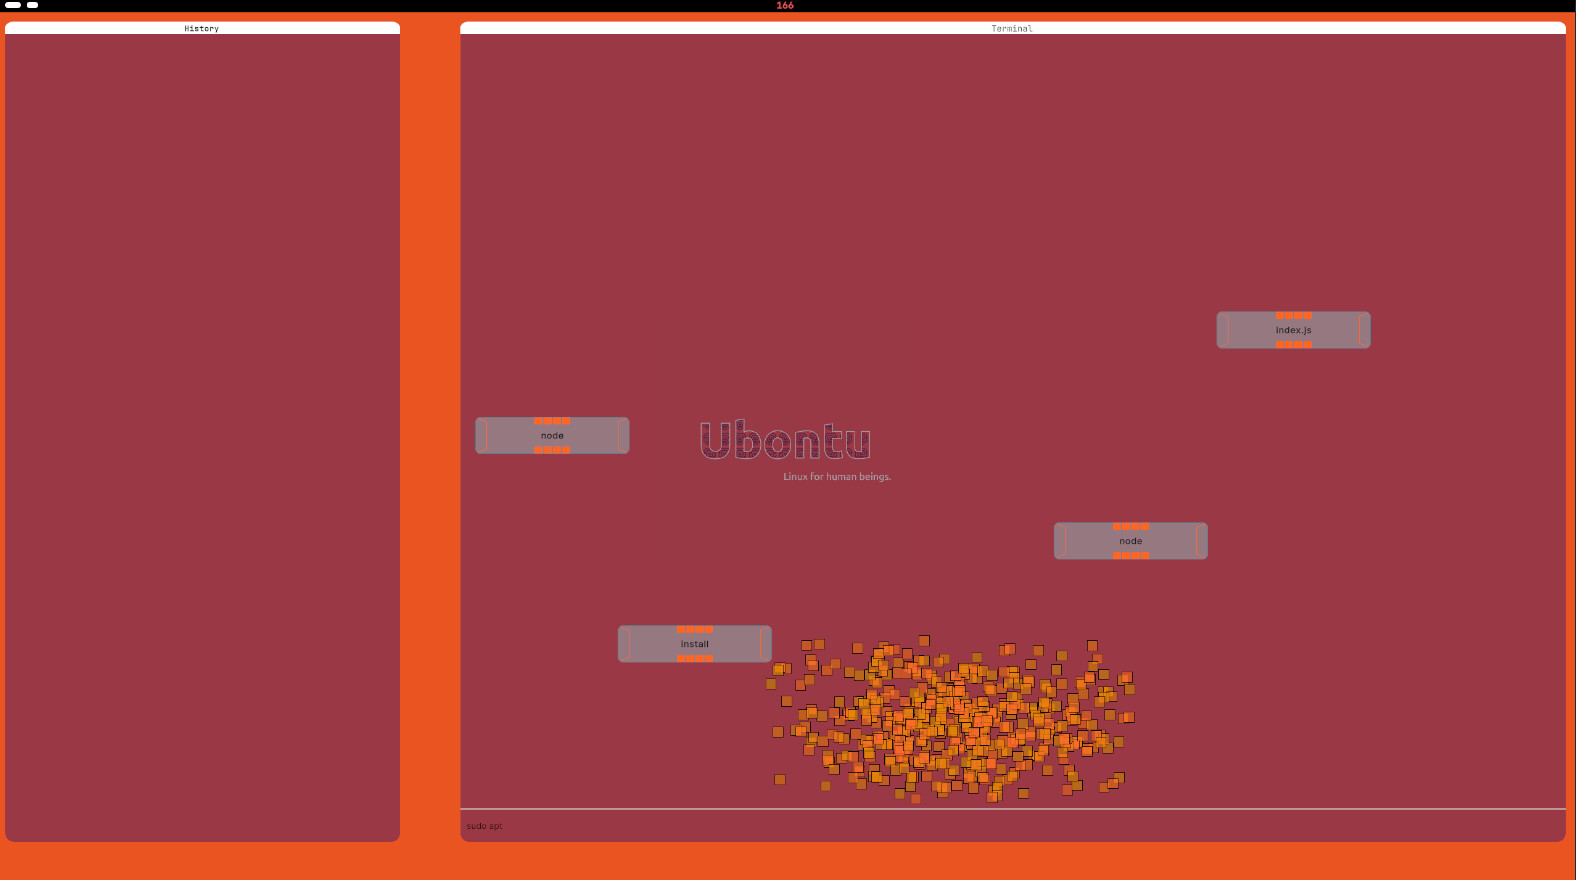
\includegraphics[width=0.65\textwidth]{images/MiniGameVFX.jpg}
    \caption{\ac{VFX} criado com o uso de \textit{frames} 2D criados com o \textit{framework} Processing.}
    \label{ProcessingVFX_WordRush}
\end{figure}

A Figura \ref{ProcessingVFX_WordRush} representa um caso prático onde os \textit{frames} criados com o \textit{framework} Processing foram utilizados para a construção de um efeito visual, quando o jogador acerta uma palavra no mini-jogo.

Além desse caso, na Figura \ref{ProcessingHomeMenu} é possível observar outro caso da utilização do Processing, onde foi utilizado para criar um conjunto de imagens 2D, as quais foram utilizadas para criar uma animação do menu principal do jogo, a qual é reproduzida quando o jogador inicia o jogo.

\begin{figure}[H]
    \centering
    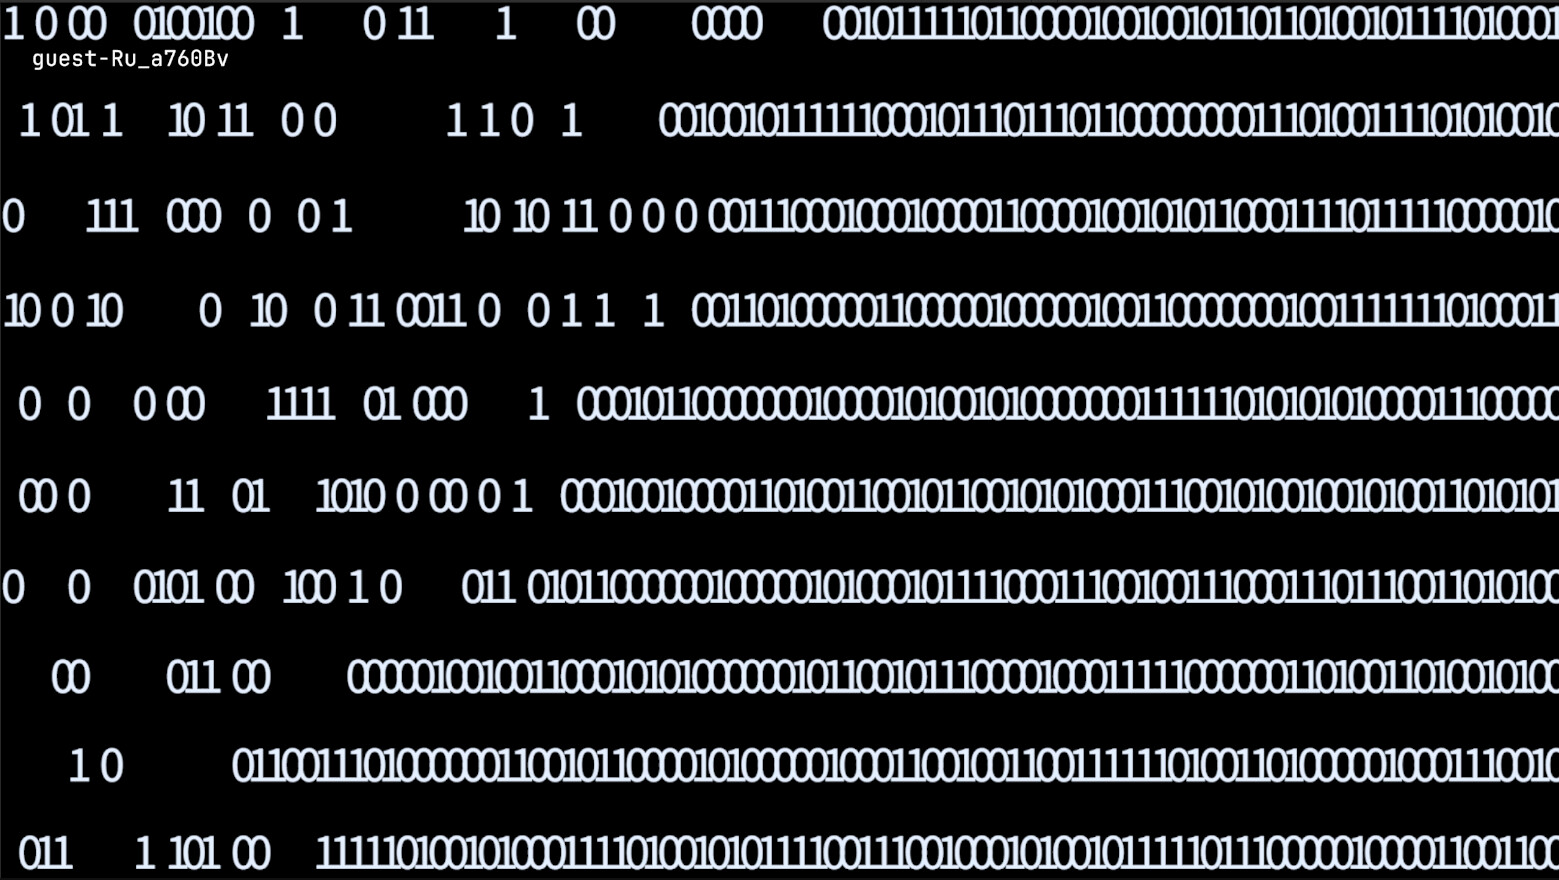
\includegraphics[width=0.65\textwidth]{images/HomeMenuEfeito.jpg}
    \caption{Animação do menu principal criada \textit{frame-by-frame} com a ajuda do \textit{framework} Processing.}
    \label{ProcessingHomeMenu}
\end{figure}

\subsection{Personagem}

\subsubsection{Modelo 3D}

\begin{figure}[H]
     \centering
     % Primeira Linha
     \begin{subfigure}[b]{0.3\textwidth}
         \centering
         
\includegraphics[width=\textwidth]{Presonagem/FurryFront.jpg}
     \end{subfigure}
     \hfill
     \begin{subfigure}[b]{0.3\textwidth}
         \centering
         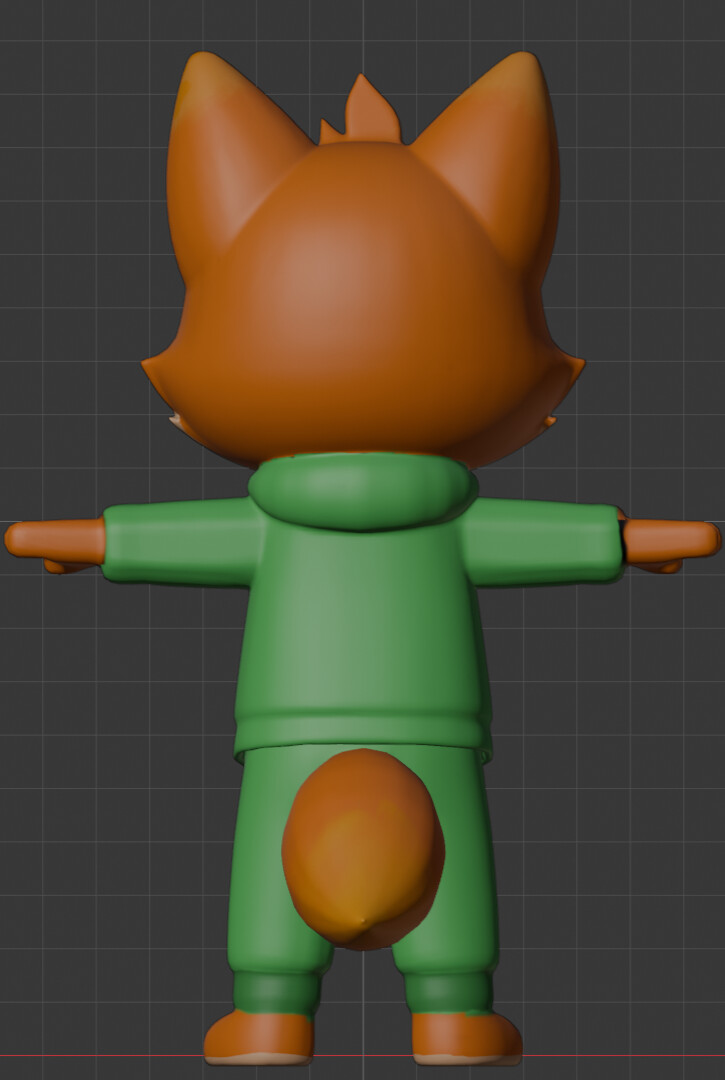
\includegraphics[width=\textwidth]{Presonagem/FurryBack.jpg}
     \end{subfigure}
     \hfill
     \begin{subfigure}[b]{0.3\textwidth}
         \centering
         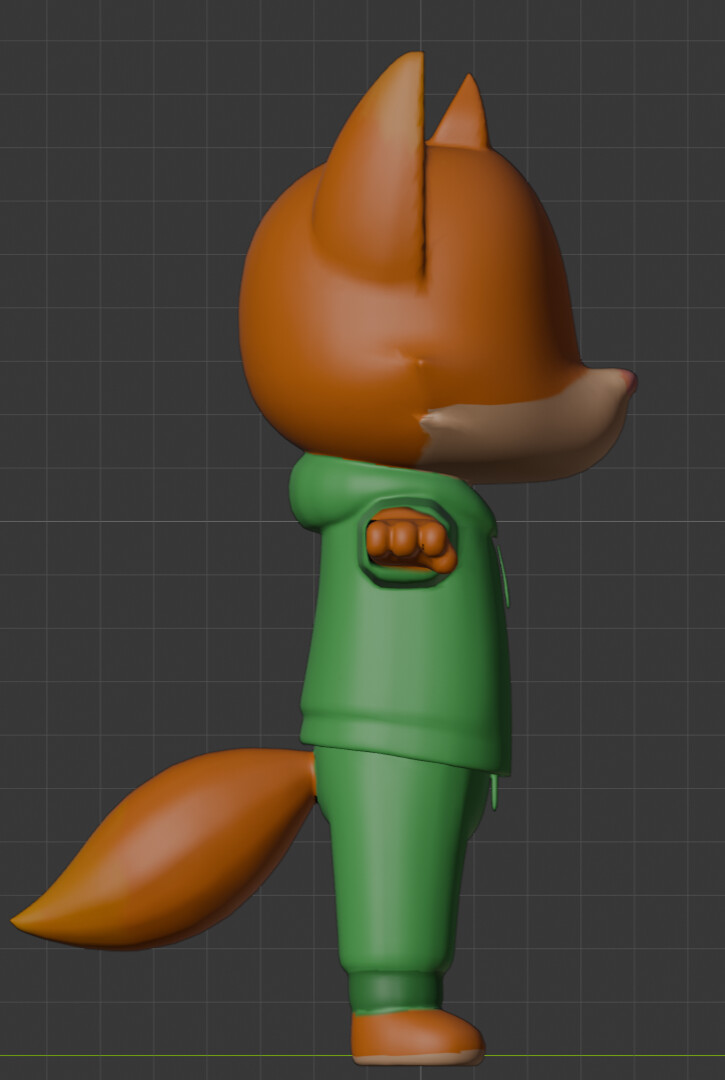
\includegraphics[width=\textwidth]{Presonagem/FurryLeft.jpg}
     \end{subfigure}

     \vspace{0.5cm} % Espaço entre as linhas

     % Segunda Linha
     \begin{subfigure}[b]{0.3\textwidth}
         \centering
         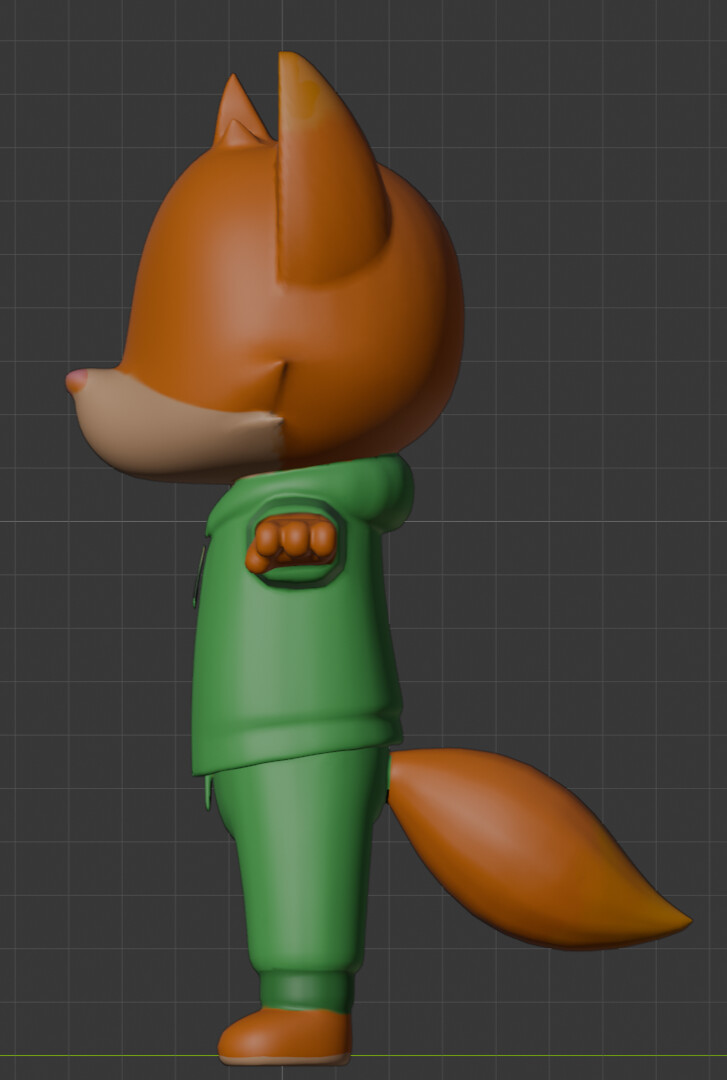
\includegraphics[width=\textwidth]{Presonagem/FurryRight.jpg}
     \end{subfigure}
     \hspace{0.5cm} % Espaço manual para centralizar a quinta imagem
     \begin{subfigure}[b]{0.3\textwidth}
         \centering
         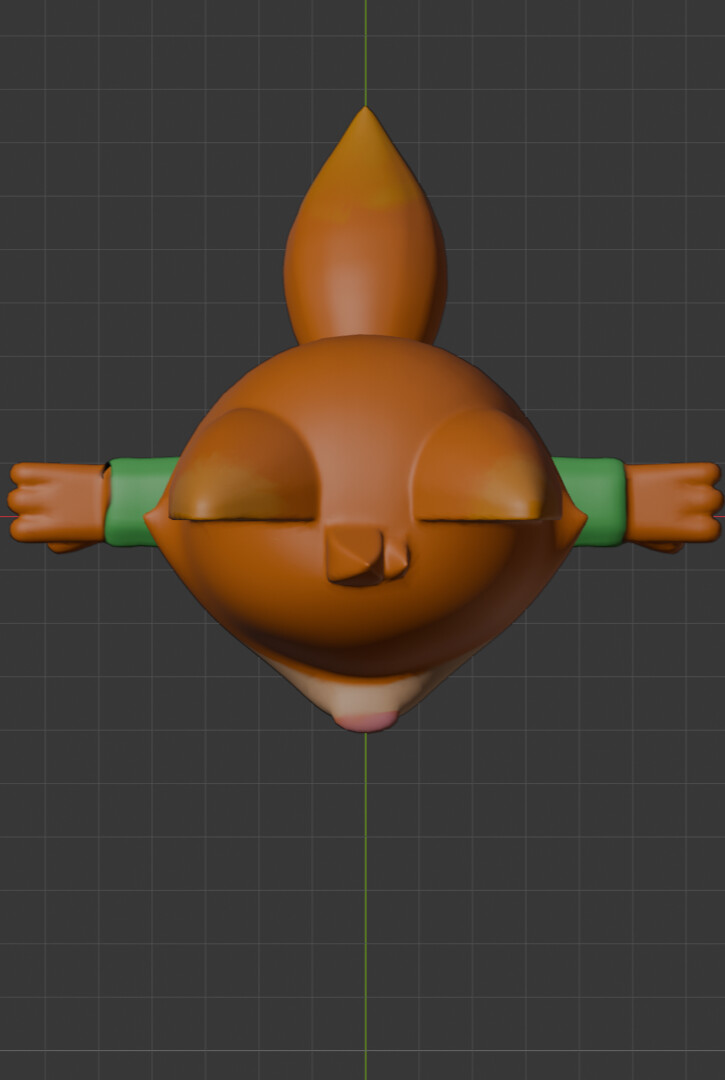
\includegraphics[width=\textwidth]{Presonagem/Furrytop.jpg}
     \end{subfigure}
     
     \caption{Modelo 3D do personagem, em várias vistas.}
     \label{characterManyLooks}
\end{figure}

O modelo 3D (\textit{mesh}) do personagem (Figura \ref{characterManyLooks}) foi criado com o auxílio da ferramenta de \ac{IA}, Chat 3D, usando como referência a Figura \ref{idealizacaoCharacter}. No entanto, a pintura de materiais e a construção de texturas, foram realizadas no \textit{software} Blender, utilizando o \textit{software} GIMP para desenvolver a textura da camisola branca.
O visual do personagem foi inspirado na mascote do \textbf{Mozilla Firefox}, uma vez que o jogo tem como tema central a internet, e o Firefox é um dos símbolos mais reconhecíveis da internet, o que faz com que seja uma fonte de inspiração bastante relevante para o projeto.

\subsubsection{Esqueleto e animações}

Um esqueleto de um modelo 3D é uma estrutura interna composta por um conjunto de “ossos” virtuais organizada de forma hierárquica, que serve para controlar a deformação e o movimento de um objeto tridimensional.

O esqueleto do modelo 3D é relevante, pois é através dele que é possível criar animações para o modelo, tais, como animações de caminhada, corrida, \textit{idel}, etc\dots.
O esqueleto do personagem foi criado no \textit{website} \textit{Mixamo}, onde também foram retidas as animações de caminhada, corrida e \textit{idle}. 

Após isso, o modelo 3D do personagem, com o esqueleto e as animações, foram importados para a Unity, onde foram feitos ajustes para que as animações pudessem ser reproduzidas de forma fluida e natural.

\subsection{Implementação do sistema de Ataque}
\label{Sec:ImplementSistemaAtaque}

\todo{Revisar}
O sistema de ataque é responsável por desencadear os ataques ao longo do jogo. Este sistema funciona de forma periódica e constante, sendo responsável pela criação dos ataques e pela instanciação dos inimigos no cenário.

Um novo ataque ocorre sempre que o jogador completa um determinado número de novas tarefas. Cada ataque encontra-se associado a um e-mail, que o jogador é obrigado a ler. O e-mail (ver Subsecção \ref{Sec:Email}) apresenta o ataque e o seu propósito, contribuindo para uma maior integração do mesmo no contexto do jogo. Para além disso, o e-mail pode também ser utilizado como meio para transmitir informação adicional ao jogador. O e-mail também atua como \textit{trigger} para a ação, enquanto o jogador não ler o e-mail o estado do jogo não se altera.

Durante o período de um ataque, o jogador pode utilizar o canhão (ver Subsecção \ref{Sec:Canhão}) presente no cenário. Para superar o ataque, o jogador terá de destruir todos os inimigos presentes no cenário.

\begin{figure}[H]
\centering

\includegraphics[width=0.65\textwidth]{images/Attack Launch.png}
\caption{Animação de início do ataque.}
\label{Launch Attack}
\end{figure}

\begin{figure}[H]
\centering
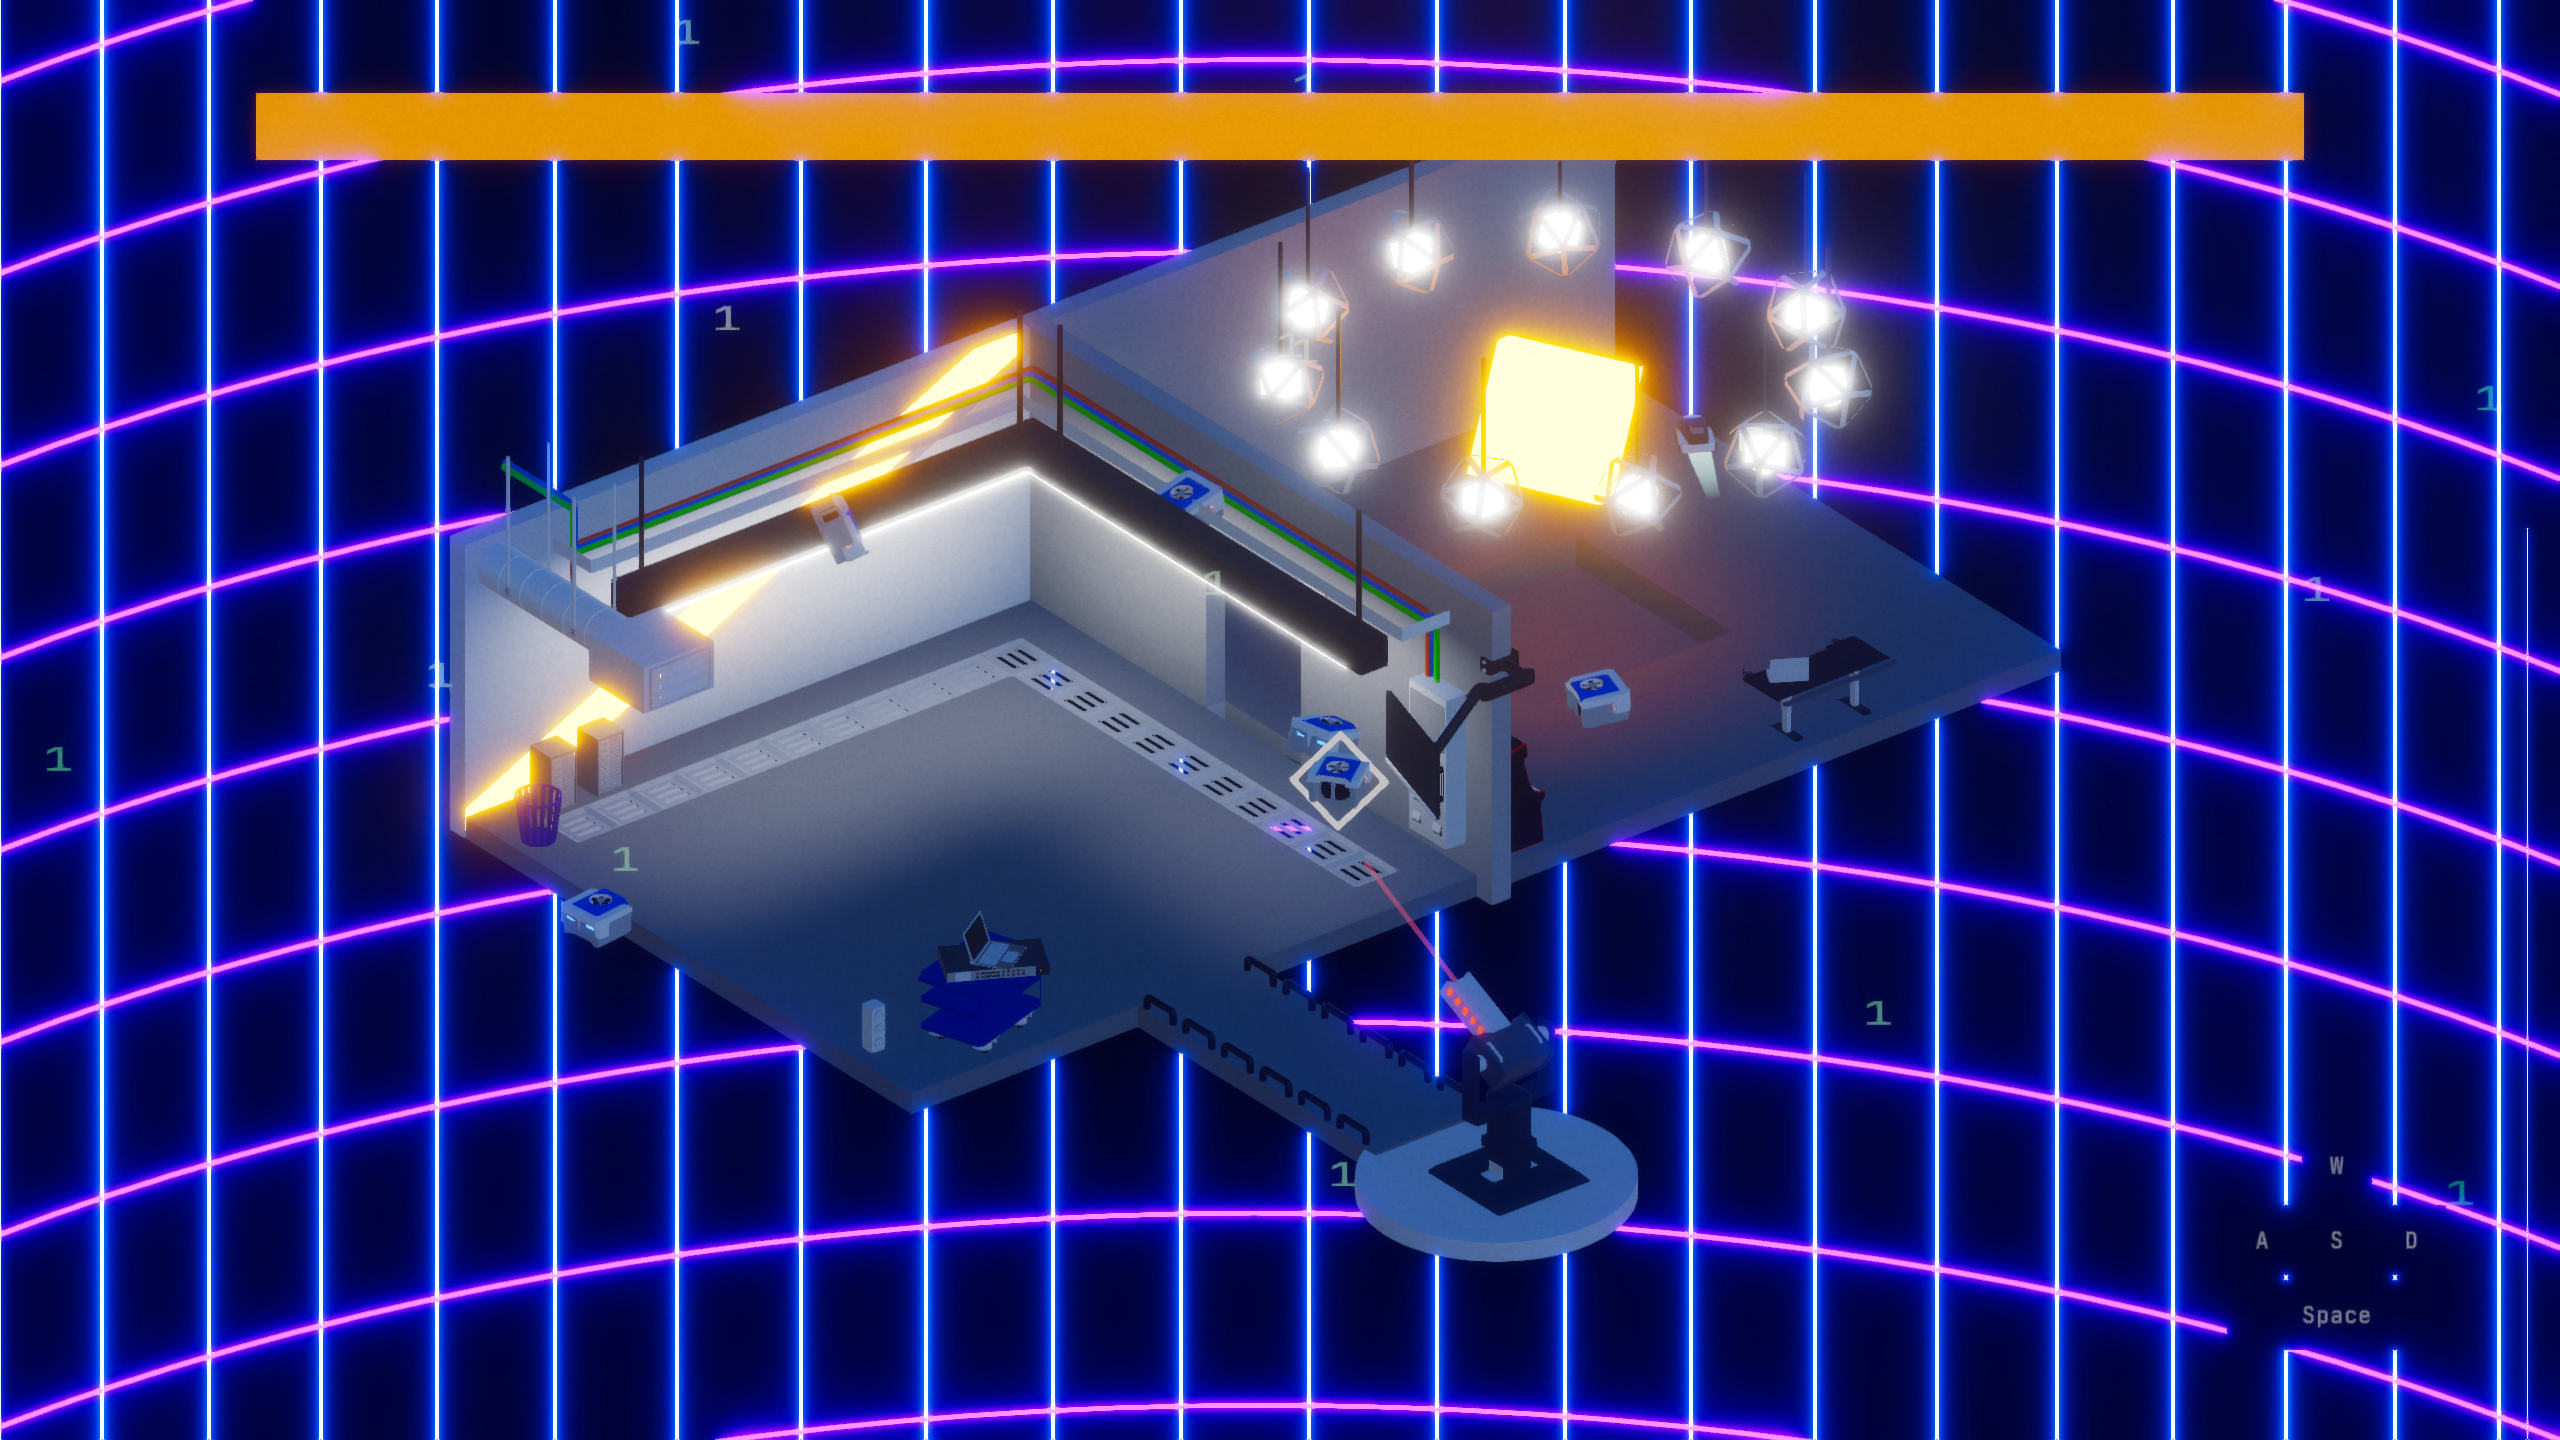
\includegraphics[width=0.65\textwidth]{images/Cannon Aim.png}
\caption{Mecânica de mira do canhão durante um ataque.}
\label{Cannon Aim}
\end{figure}

A Figura \ref{Launch Attack} representa a animação apresentada sempre que se inicia um novo ataque. A principal função desta animação é contextualizar o jogador relativamente ao ataque que se inicia, apresentando o seu nome e permitindo-lhe preparar-se para a invasão. Durante esta animação, o estado do mundo permanece inalterado, garantindo ao jogador um período de preparação antes do início do ataque.

A Figura \ref{Cannon Aim} representa a perspetiva do jogador durante um ataque. Neste contexto, o jogador deixa de controlar diretamente a personagem e passa a controlar o canhão presente no cenário. Na parte superior do ecrã encontra-se uma barra centralizada que representa a percentagem de inimigos que ainda permanecem no cenário. Assim, quanto menor for o valor apresentado, menor será o número de inimigos que falta destruir.

Uma vez que a câmara utilizada neste \textit{minijogo} é a mesma utilizada no restante jogo, sendo esta uma câmara ortográfica, não existe perspetiva nem perceção de profundidade através da escala dos objetos. Esta característica torna a tarefa de apontar mais difícil, pelo que foram implementados mecanismos adicionais para facilitar a mira. Na extremidade do canhão foi adicionado um laser que funciona como auxiliar de mira. Adicionalmente, quando a mira se encontra sobre um inimigo, é apresentado um indicador branco à sua volta, permitindo identificar de forma mais clara o alvo selecionado.

Estas funcionalidades foram implementadas com o objetivo de melhorar a experiência de mira do jogador, compensando a ausência de perspetiva e, consequentemente, a reduzida perceção de profundidade proporcionada pela câmara ortográfica.

Para compreender melhor a forma como o sistema de ataque interage com os restantes sistemas do jogo, podem ser consultadas as Subsecções \ref{Sec:DiagramaSistemaJogo} e \ref{Sec:Canhão}.


\todo{Até Aqui}

\subsection{Implementação do \textit{WordRush}}
\label{Sec:WordRush}

\todo{Revisar}
O \textit{WordRush} é o principal \textit{minigame} presente no projeto, uma vez que é responsável por simular a execução das tarefas. A sua utilização ocorre como consequência direta da aceitação de uma tarefa, que é comunicada ao jogador através de uma notificação (consultar a Secção \ref{Sec:Notify} para mais informações sobre o sistema de notificações).

O objetivo deste \textit{minigame} é simular um terminal no qual o jogador deve escrever um conjunto de palavras que surgem no ecrã e que, quando corretamente introduzidas, permitem a execução de comandos. Estes comandos estão diretamente relacionados com o tipo de tarefa previamente aceite pelo jogador. Em termos visuais, a interface foi inspirada no ambiente gráfico \textit{GNOME} (ver Subsecção \ref{Sec:ReferenciasReais}) e no jogo \textit{Grey Hack} (ver Subsecção \ref{Sec:GreyHack}).

Como pode ser observado na Figura \ref{WordRush Current}, a interface do \textit{WordRush} encontra-se dividida em três áreas principais. A área central direita corresponde à zona onde as palavras surgem e se deslocam pelo ecrã. Na zona inferior direita encontra-se o campo de introdução, onde o jogador escreve as palavras apresentadas. Por sua vez, a área lateral esquerda apresenta os comandos que foram introduzidos pelo jogador, acompanhados de uma breve descrição da função de cada um.

As palavras apresentadas ao jogador variam de acordo com o tipo de tarefa que está a ser executada, sendo igualmente atribuída uma pontuação (\textit{score}) distinta consoante as palavras ou comandos introduzidos. Desta forma, o \textit{WordRush} adapta a sua jogabilidade ao contexto da tarefa, permitindo representar diferentes tipos de atividades através de uma mesma mecânica de interação.

\begin{figure}[H]
\centering
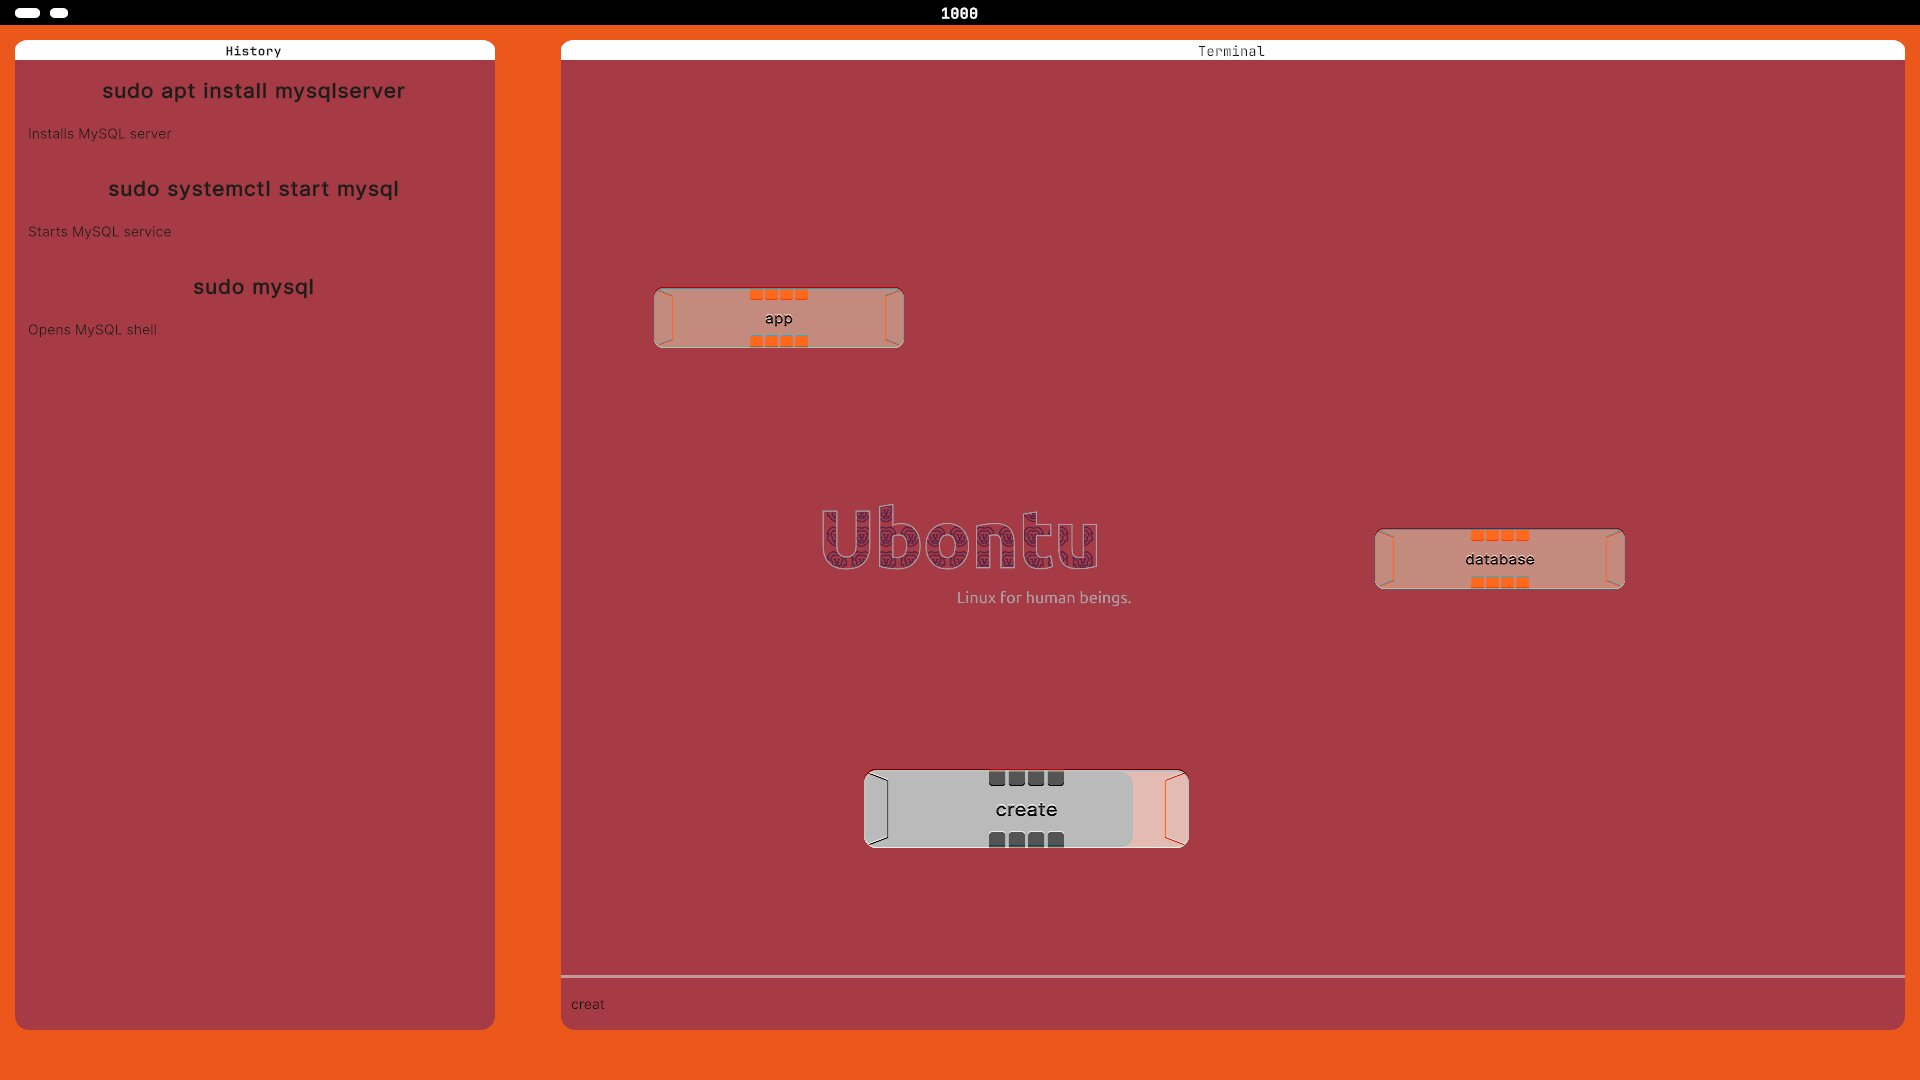
\includegraphics[width=0.65\textwidth]{images/WordRush.jpg}
\caption{\textit{Minigame WordRush}.}
\label{WordRush Current}
\end{figure}

\begin{figure}[H]
\centering
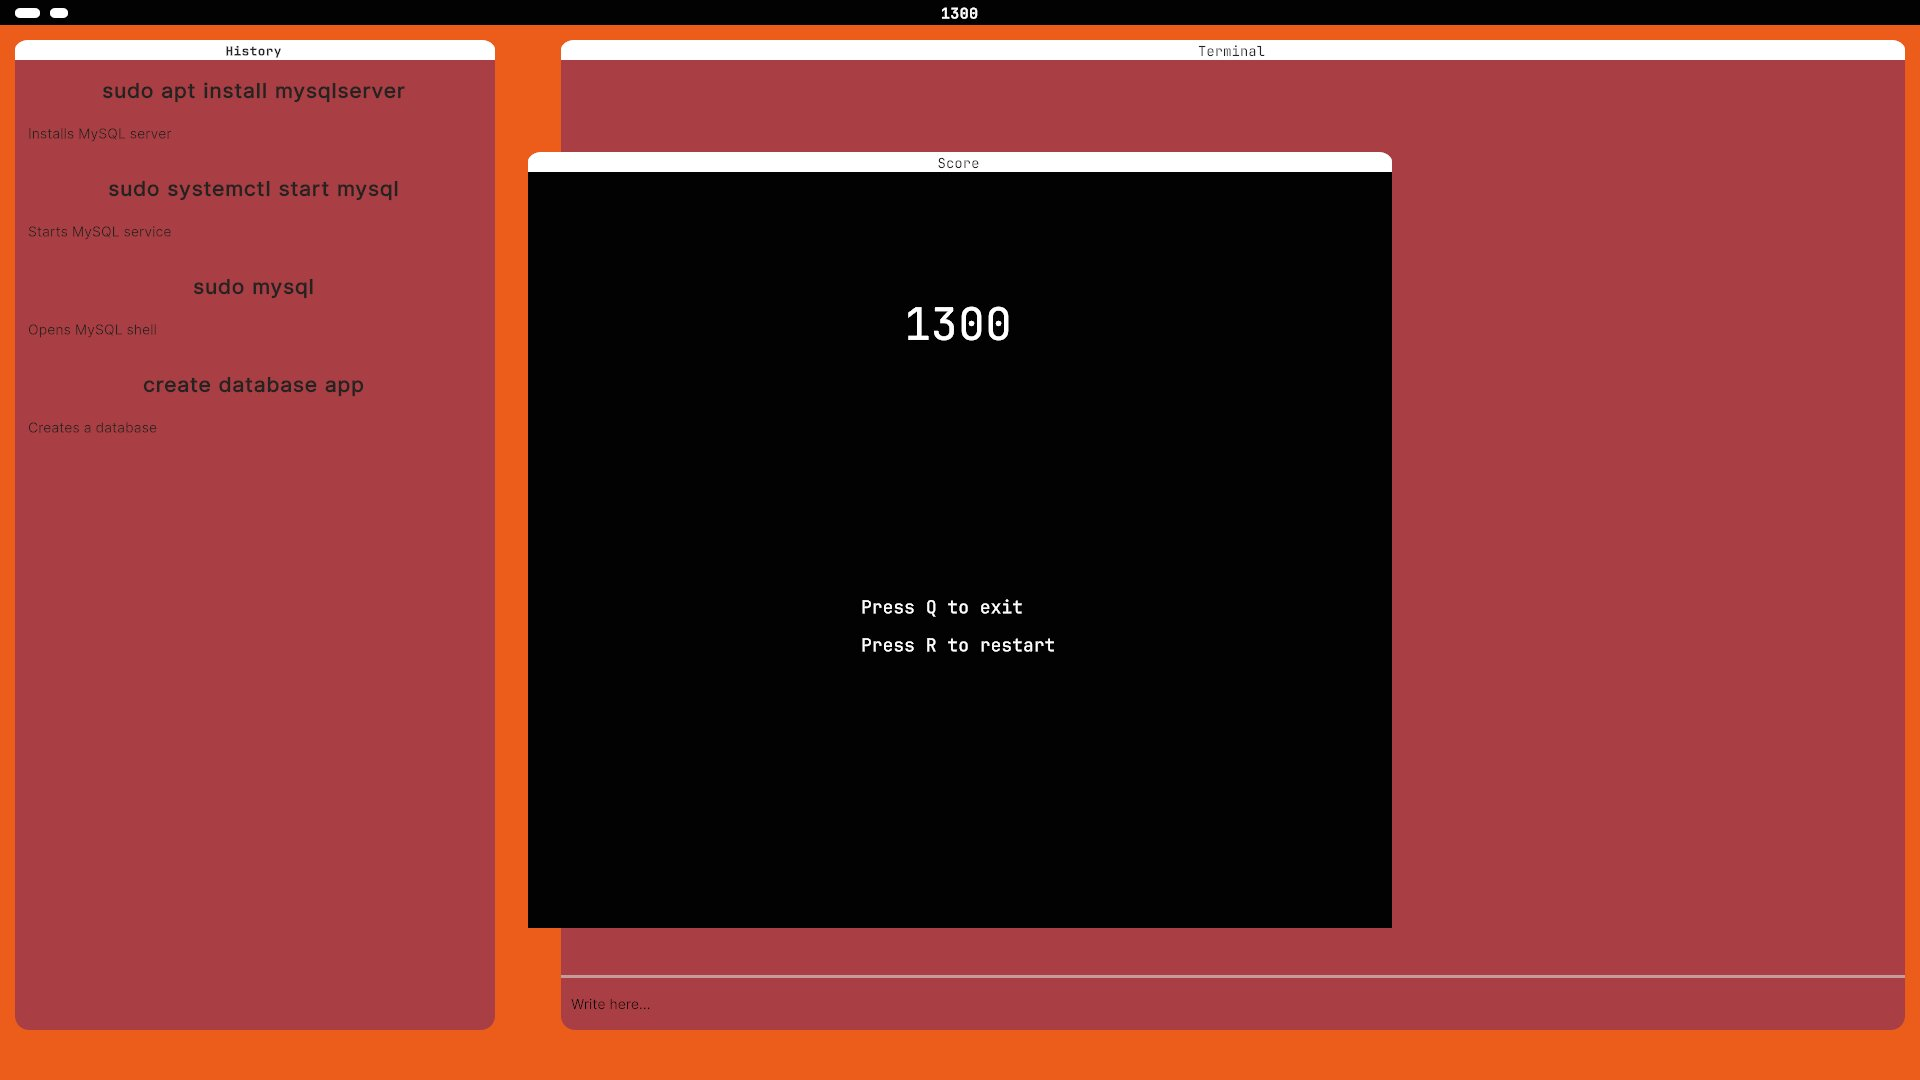
\includegraphics[width=0.65\textwidth]{images/WordRushFinished.jpg}
\caption{Tela final do \textit{minigame WordRush}.}
\label{WordRush Finished}
\end{figure}

\todo{Aqui}

\chapter{Testes e Avaliação do Jogo}

\label{cap5}

\todo{Analisar}

Com o objetivo de analisar o projeto desenvolvido, foram aplicados dois formulários: um antes da sessão de jogo e outro após a sua conclusão. O objetivo destes formulários consiste em avaliar se existe um aumento dos conhecimentos dos participantes após a experiência de jogo. O objetivo do jogador durante o teste é chegar até ao 1º ataque de \textit{DDos}.

Em simultâneo, as sessões de jogo de cada participante foram analisadas com o objetivo de identificar padrões de utilização e oportunidades de melhoria ao nível da \ac{UX}. Os dados recolhidos durante estas sessões foram analisados com base nas heurísticas de usabilidade propostas por \textcite{nielsen1994enhancing}, cuja aplicação será detalhada nas subsecções seguintes.

A escolha destas heurísticas como métrica de avaliação deve-se à natureza dos dados em análise, uma vez que estas foram desenvolvidas especificamente para avaliar a experiência do utilizador.

Para além das métricas anteriormente referidas, foram ainda recolhidos dados de telemetria de forma automática durante cada sessão de jogo. Para esse efeito, foi utilizada a plataforma \textbf{Firebase} para armazenar essa informação. O objetivo desta recolha consiste em identificar padrões relacionados com os tempos de interação dos jogadores em diferentes situações, permitindo perceber se existem momentos da \textit{gameplay} que apresentam comportamentos significativamente discrepantes relativamente aos restantes.

\section{Analise qualitativa da \ac{UX}}

\begin{table}[H]
    \centering
    \begin{tabular}{|p{4.5cm}|c|p{3cm}|p{4.5cm}|}
        \hline
        \textbf{Problema} & \textbf{Grau} & \textbf{Heuristica} & \textbf{Solução} \\ \hline
        Falta de \textit{feedback} no sistema de som & Baixo & Visibilidade do estado do sistema & Adição uma \textit{label} informativa \\ \hline
        Falta de \textit{feedback} nos botões de notificações & Média & Visibilidade do estado do sistema & Adição de instruções mais claras ao lado dos botões \\ \hline
        Controlos do canhão & Elevado & Controlos do utilizador e liberdade / Consitência e padronização & Inverter os commandos \\ \hline
        Jogador não se lembra como abrir a loja & Elevado & Reconhecimento em vez de memorização & Adição de indicativo visual na \ac{UI}. \\ \hline
        Jogador não têm noção da finalidade dos componentes de \textit{hardware} & Elevado & Correspondência entre o sistema e o mundo & Adição de uma label com uma pequena descrição do componente na loja \\ \hline
        Falta de \textit{feedback} na configuração de um \ac{CPU} na tela da loja & Media & Visibilidade do estado do sistema & Adição de uma \textit{label} informativa. \\ \hline
        Falta de \textit{feedback} nos emails & Elevado & Visibilidade do estado do sistema & Adição de um idicador visual, que aparece sempre que existe um email por ler \\ \hline
        Câmara muito próxima do jogador & Baixo & Controlo e liberdade do jogador & Adição do controlo de zoom da câmara \\ \hline
    \end{tabular}
    \caption{Analise dos problemas usando as heuristicas de Nielsen}
    \label{tab:DadosNielsen}
\end{table}

Os dados recolhidos das observações das seções de jogo de dos jogadores que participaram nos testes encontrassam analisados
na tabela \ref{tab:DadosNielsen}.

\section{Analisa do conhecimento transmitido e das seções de jogo}

Esta seção é divida em várias sub seções, onde são analisados os dados recolhidos oriundos dos formulários assim como os dados de telemetria recolhidos ao logo de cada seção de jogo, tais como:
\begin{itemize}
    \item Tempo para comprar/configurar o 1º servidor;
    \item Tempo necessário para concluir cada mini game;
    \item Watts do servidores;
    \item Tempo que o jogador demorou para destruir o 1º ataque \textit{DDos};
    \item Tempo total da seção de jogo até a finalização do 1º ataque.
\end{itemize}

\subsection{Defenição da amostra}

A amostra utiliza para realizar um dado teste é facto primário que avalia a qualidade do mesmo, uma vez que se a amostra for muito pequena os resultados derivados dela podem não refletir a relidade de uma dada população (conjunto total de indivíduos ou objectos sobre os quais incide o estudo). Além do seu tamanho, uma boa amostra também deve ser diversas, uma vez que se uma amostra for pouco diversa ela irá gera viés estatísticos.

Posto isto a amostra recolhida para desenvolver os testes, é composta de um total de 25 individuos, de vários gêneros, e com uma faixa etária que varia desde [menos 18 anos até mais de 30 anos]. A seguir serão apresentados um conjunto de dados tabulares e em gráficos que a caracterização.

\begin{table}[H]
    \centering
    \begin{tabular}{|c|c|}
        \hline
        \textbf{Faixa de idades} & \textbf{Número de individuos} \\ \hline
        Menos de 18 anos & 2 \\ \hline
        18 a 24 anos & 10 \\ \hline
        25 a 29 anos & 11 \\ \hline
        30 a 34 anos & 2 \\ \hline
        Mais de 35 anos & 0 \\ \hline
    \end{tabular}
    \caption{Faixa de idades}
    \label{tab:Faixa_Idades}
\end{table}


A Tabela \ref{tab:Faixa_Idades} informa que maioria dos individuos se encontram entre os 18 e 29 anos, todavia, existe um pequeno conjunto que se encontra fora desse intrevalo.


\begin{table}[H]
    \centering
    \begin{tabular}{|c|c|}
        \hline
        \textbf{Conhecimentos em informática} & \textbf{Número de individuos} \\ \hline
        Possuir e tem formação académica na área da informática & 13 \\ \hline
        Apenas na ótica do utilizador & 4 \\ \hline
        Não possuir & 7 \\ \hline
    \end{tabular}
    \caption{Conhecimentos prévios em informática}
    \label{tab:Conhecemintos}
\end{table}

A partir da Tabela \ref{tab:Conhecemintos}, conclui-se que 52\% da amostra possui formação na área, enquanto os restantes 48\% não possuem qualquer formação ou possuem apenas formação na ótica do utilizador. Este dado é importante para interpretar o conhecimento prévio dos participantes, uma vez que os indivíduos que já possuem conhecimentos na área poderão não apresentar um incremento significativo.

\begin{figure}[H]
    \centering
    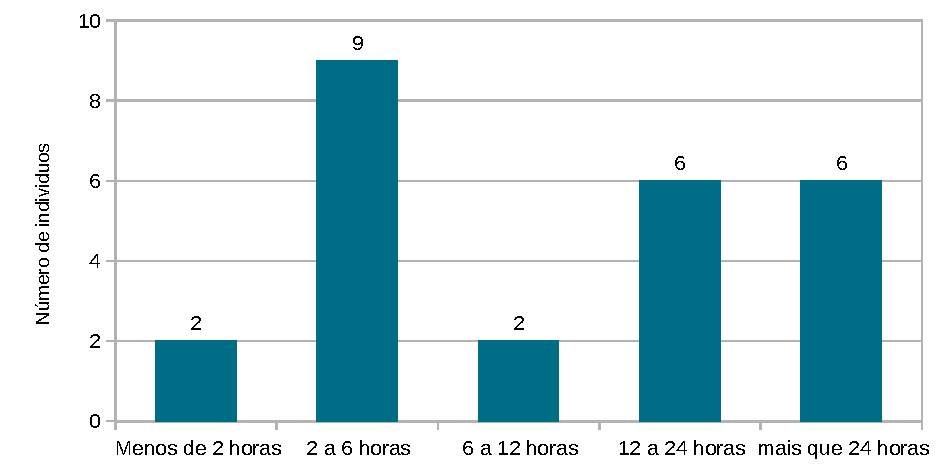
\includegraphics[width=0.8\textwidth]{images/Gráficos dos testes/Graficos de horas.pdf}
    \caption{Número de horas semanais dispensadas para jogar}
    \label{graph:Numero_Horas_Semanais}
\end{figure}

A partir do gráfico apresentado na Figura \ref{graph:Numero_Horas_Semanais}, verifica-se que a amostra é constituída por jogadores com diferentes níveis de horas. Esta variedade poderá influenciar os resultados obtidos, sobretudo ao nível da \ac{UX}, uma vez que os jogadores que dedicam mais horas aos videojogos tendem a desenvolver um repertório mais alargado de experiências e referências neste domínio. Consequentemente, poderão apresentar uma maior facilidade de adaptação quando confrontados com novos cenários, neste caso, um novo videojogo.



%\setcounter{secnumdepth}{+2}
\chapter{Conclusões e Trabalho Futuro}
\label{cap6}

\todo{Revisar}

Este capítulo encerra o presente relatório de projeto, apresentando uma síntese das principais conclusões retiradas ao longo do processo de desenvolvimento e avaliação do videojogo. São igualmente detalhadas as principais contribuições resultantes deste trabalho, assim como as linhas de investigação e desenvolvimento futuro que visam dar continuidade ao projeto.

\section{Conclusões}
\label{sec6_1}

O principal objetivo deste projeto consistiu no design e implementação de um videojogo de simulação e gestão de infraestruturas tecnológicas, que procurou equilibrar o rigor técnico de conceitos reais de computação com o entretenimento e o empenho lúdico do jogador.

Os resultados obtidos através da aplicação de testes com utilizadores e da análise de telemetria permitiram validar a eficácia da abordagem adotada. Em primeiro lugar, demonstrou-se que o jogo foi capaz de transmitir e reforçar conhecimentos técnicos sobre informática e \textit{data centers} de forma orgânica. Verificou-se um aumento notável no reconhecimento de conceitos-chave, tais como a arquitetura de processadores ARM (que passou de $56\%$ para $84\%$), o papel da IBM no desenvolvimento de CPUs para servidores, a importância do sistema operativo Linux e a utilização de \textit{frameworks} (como o Apache) para alojamento \textit{web}.

Em segundo lugar, a avaliação da experiência do utilizador (UX) e do fluxo de jogo (\textit{flow}) comprovou que a inclusão de elementos mecânicos alternativos, como o \textit{minigame} de terminal \textit{WordRush} e os momentos de combate para contenção de ataques cibernéticos (DDoS), desempenhou um papel determinante na quebra da monotonia associada à pura gestão económica. A alternância entre momentos de planeamento estratégico e desafios dinâmicos manteve os jogadores motivados, garantindo um equilíbrio adequado entre desafio e aprendizagem.

Não obstante as limitações identificadas durante os testes de usabilidade, designadamente ao nível da perceção espacial na perspetiva isométrica e da necessidade de otimização de alguns indicadores de \textit{feedback} visual e sonoro, o protótipo funcional desenvolvido atingiu com sucesso as metas propostas, servindo como uma prova de conceito sólida para a utilização de jogos comerciais e casuais como veículos de aprendizagem indireta.

\section{Contribuições}
\label{sec6_2}

O desenvolvimento do presente projeto de mestrado resultou num conjunto de contribuições práticas, concetuais e técnicas na área do design e desenvolvimento de jogos digitais aplicados à simulação tecnológica:

\begin{itemize}
    \item \textbf{Protótipo Funcional e Integrado:} Desenvolvimento de um videojogo 3D funcional na \textit{engine} Unity, integrando sistemas complexos de economia contínua em tempo real, simulação de parâmetros energéticos (Watts) e capacidade de processamento (TFLOPS), e mecânicas de combate dinâmico.
    \item \textbf{\textit{Framework} de Aprendizagem Indireta em Sistemas de TI:} Conceção e validação de um modelo de design de jogo que traduz infraestruturas e conceitos teóricos de redes, \textit{hardware} e sistemas operativos em mecânicas lúdicas envolventes, comprovando a eficácia da transmissão de conhecimento técnico sem comprometer a vertente recreativa.
    \item \textbf{Recursos de Arte 3D e Animação 2D Original:} Criação de um conjunto de \textit{assets} tridimensionais (modelos do cenário, \textit{racks} de servidores, equipamento de rede e canhão) constuidos no Blender, combinados com um fluxo de trabalho inovador que envolveu ferramentas de Inteligência Artificial e a \textit{framework} Processing para animação 2D e \ac{VFX} visuais.
    \item \textbf{Mecânica Adaptativa de Terminal (WordRush):} Design e implementação do \textit{minigame} \textit{WordRush}, que simula a execução de comandos de terminal com base em \textit{typing}, adaptando dinamicamente a pontuação, sintaxe e vocabulário ao tipo de tarefa contratada pelos clientes no jogo.
    \item \textbf{Estudo de Avaliação e Telemetria:} Análise detalhada do comportamento do utilizador através da integração com o Google Firebase, combinada com formulários antes e após o jogo e avaliação heurística de Nielsen, disponibilizando dados empíricos sobre a retenção de conhecimento e padrões de usabilidade em simuladores de TI.
\end{itemize}

\section{Trabalho Futuro}
\label{sec6_3}

Embora o protótipo desenvolvido tenha cumprido com êxito os objetivos propostos para esta dissertação, identificam-se diversas oportunidades de expansão e melhoria que podem ser exploradas em trabalhos futuros:

\begin{itemize}
    \item \textbf{Implementação do Sistema de Progressão Narrativa:} Integrar na totalidade a narrativa idealizada no conceito inicial, incluindo a obtenção da chave criptográfica de controlo do tempo como recompensa final ao atingir o nível máximo de expansão do \textit{data center}.
    \item \textbf{Aprofundamento do Sistema de RPG e Personagens:} Evoluir o sistema de combate atual (baseado na mecânica do canhão e eliminação de \textit{drones}) para o modelo original inspirado em jogos RPG, introduzindo \textit{builds} de equipamentos, atributos técnicos (largura de banda, algoritmos de encriptação, capacidade de processamento) e árvores de competências.
    \item \textbf{Área de Customização e Troféus (Área 2):} Concluir a implementação da Área 2 do \textit{level design}, permitindo ao jogador personalizar o espaço físico do \textit{data center}, adquirir elementos decorativos e exibir conquistas/troféus alcançados ao longo do progresso no jogo.
    \item \textbf{Complexidade Adicional na Simulação Económica e Ambiental:} Introduzir variáveis de gestão avançadas que foram simplificadas nesta versão, nomeadamente a gestão individualizada de sistemas de arrefecimento (CRACs/corredores quentes e frios), custos de abastecimento de água, largura de banda de internet contratada e redundância de energia (UPS e geradores).
    \item \textbf{Melhorias de Usabilidade e Acessibilidade (UX/UI):} Corrigir os problemas identificados no estudo qualitativo de UX (Tabela \ref{tab:DadosNielsen}), aperfeiçoando os controlos e indicação de mira do canhão, ajustando a câmara ortográfica com zoom dinâmico e adicionando indicadores visuais e sonoros persistentes para notificações de e-mail e atalhos de teclado.
    \item \textbf{Expansão da Variedade de Ataques Cibernéticos:} Introduzir novos tipos de ameaças de segurança no ecossistema de jogo, tais como ataques de \textit{Ransomware}, \textit{Phishing} ou usurpação de portas de rede, ampliando a variedade de \textit{puzzles} e reforçando a literacia em cibersegurança dos utilizadores.
\end{itemize}




\backmatter

%\renewcommand{\bibname}{References}
\printbibliography

\appendix

\chapter{Anexos}

% Anexo A
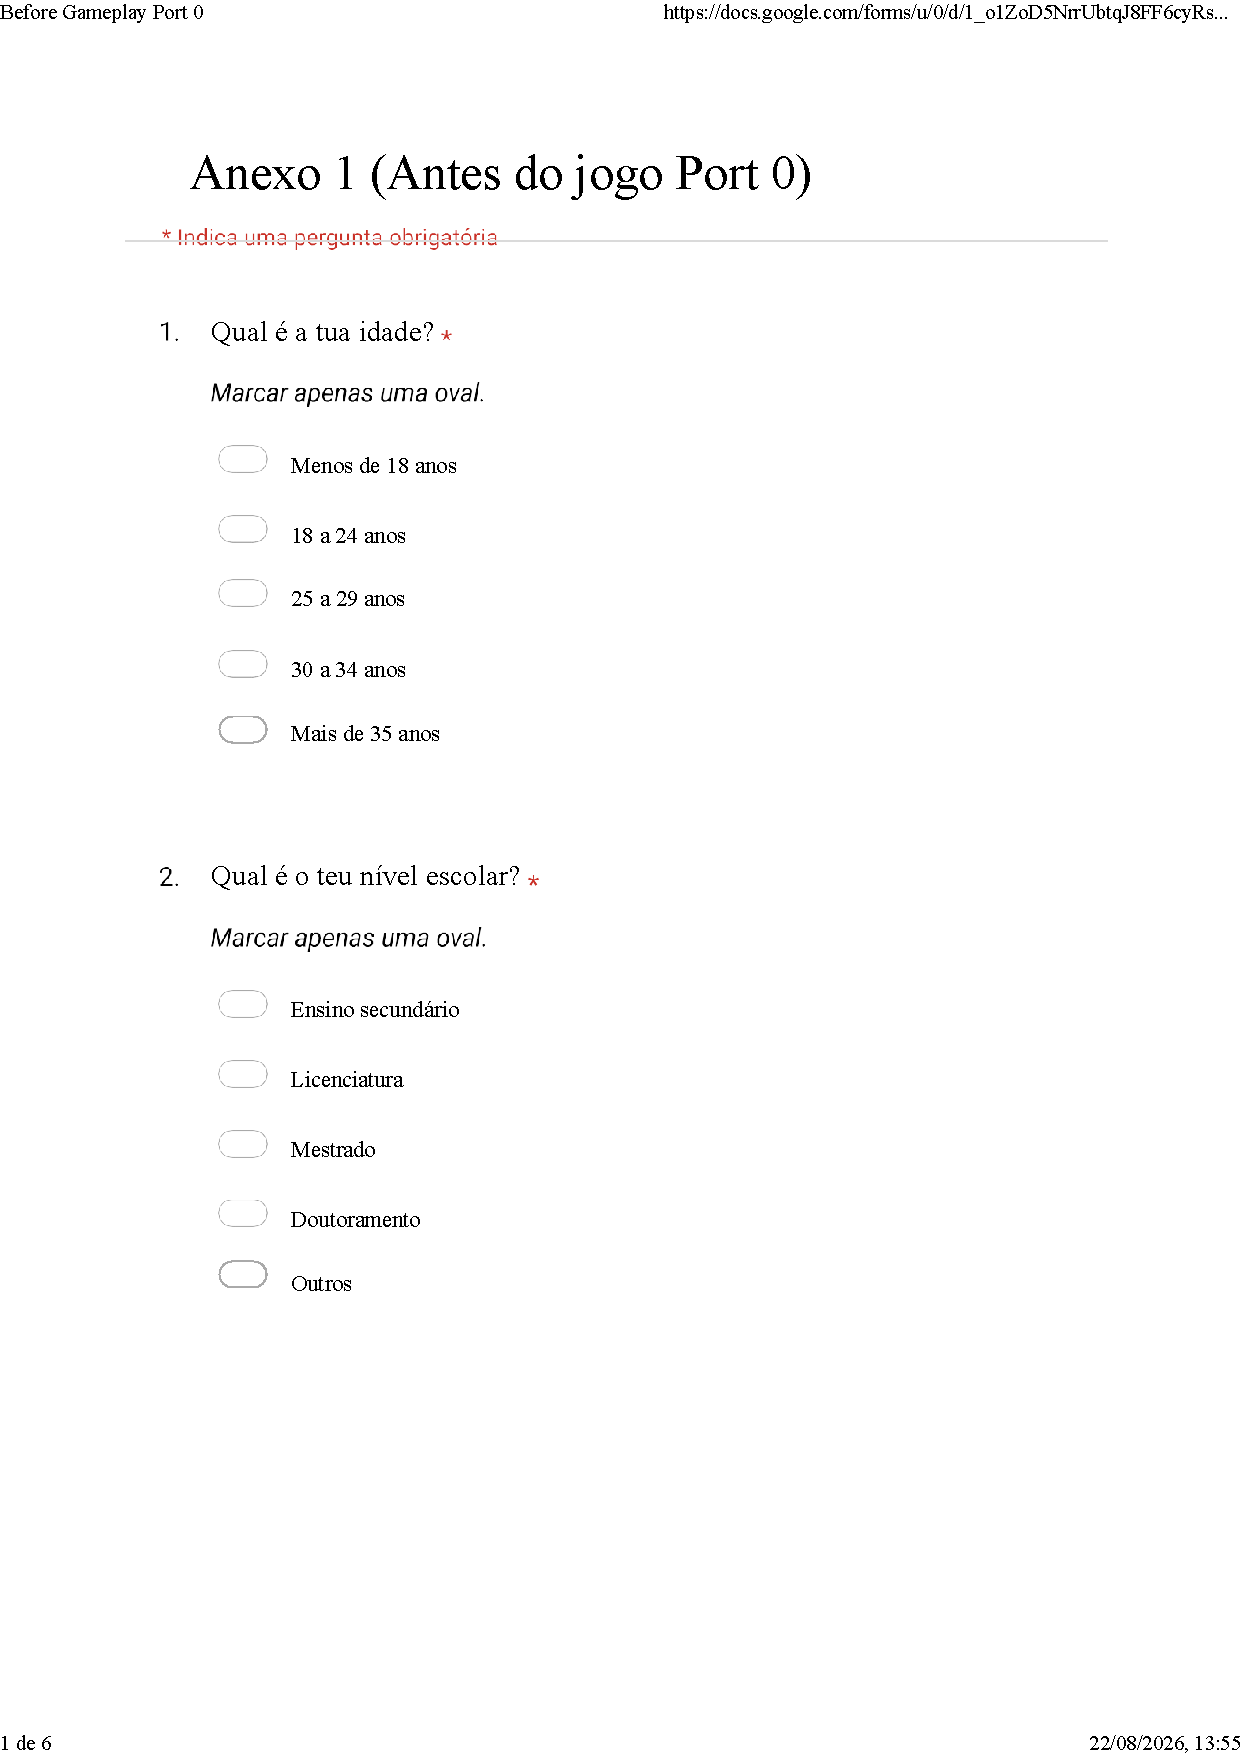
\includepdf[
  pages=-,
  pagecommand={
    \refstepcounter{section}\label{Anexo:antes_jogo}
  },
  scale=0.8
]{./forms/before.pdf}

% Anexo B
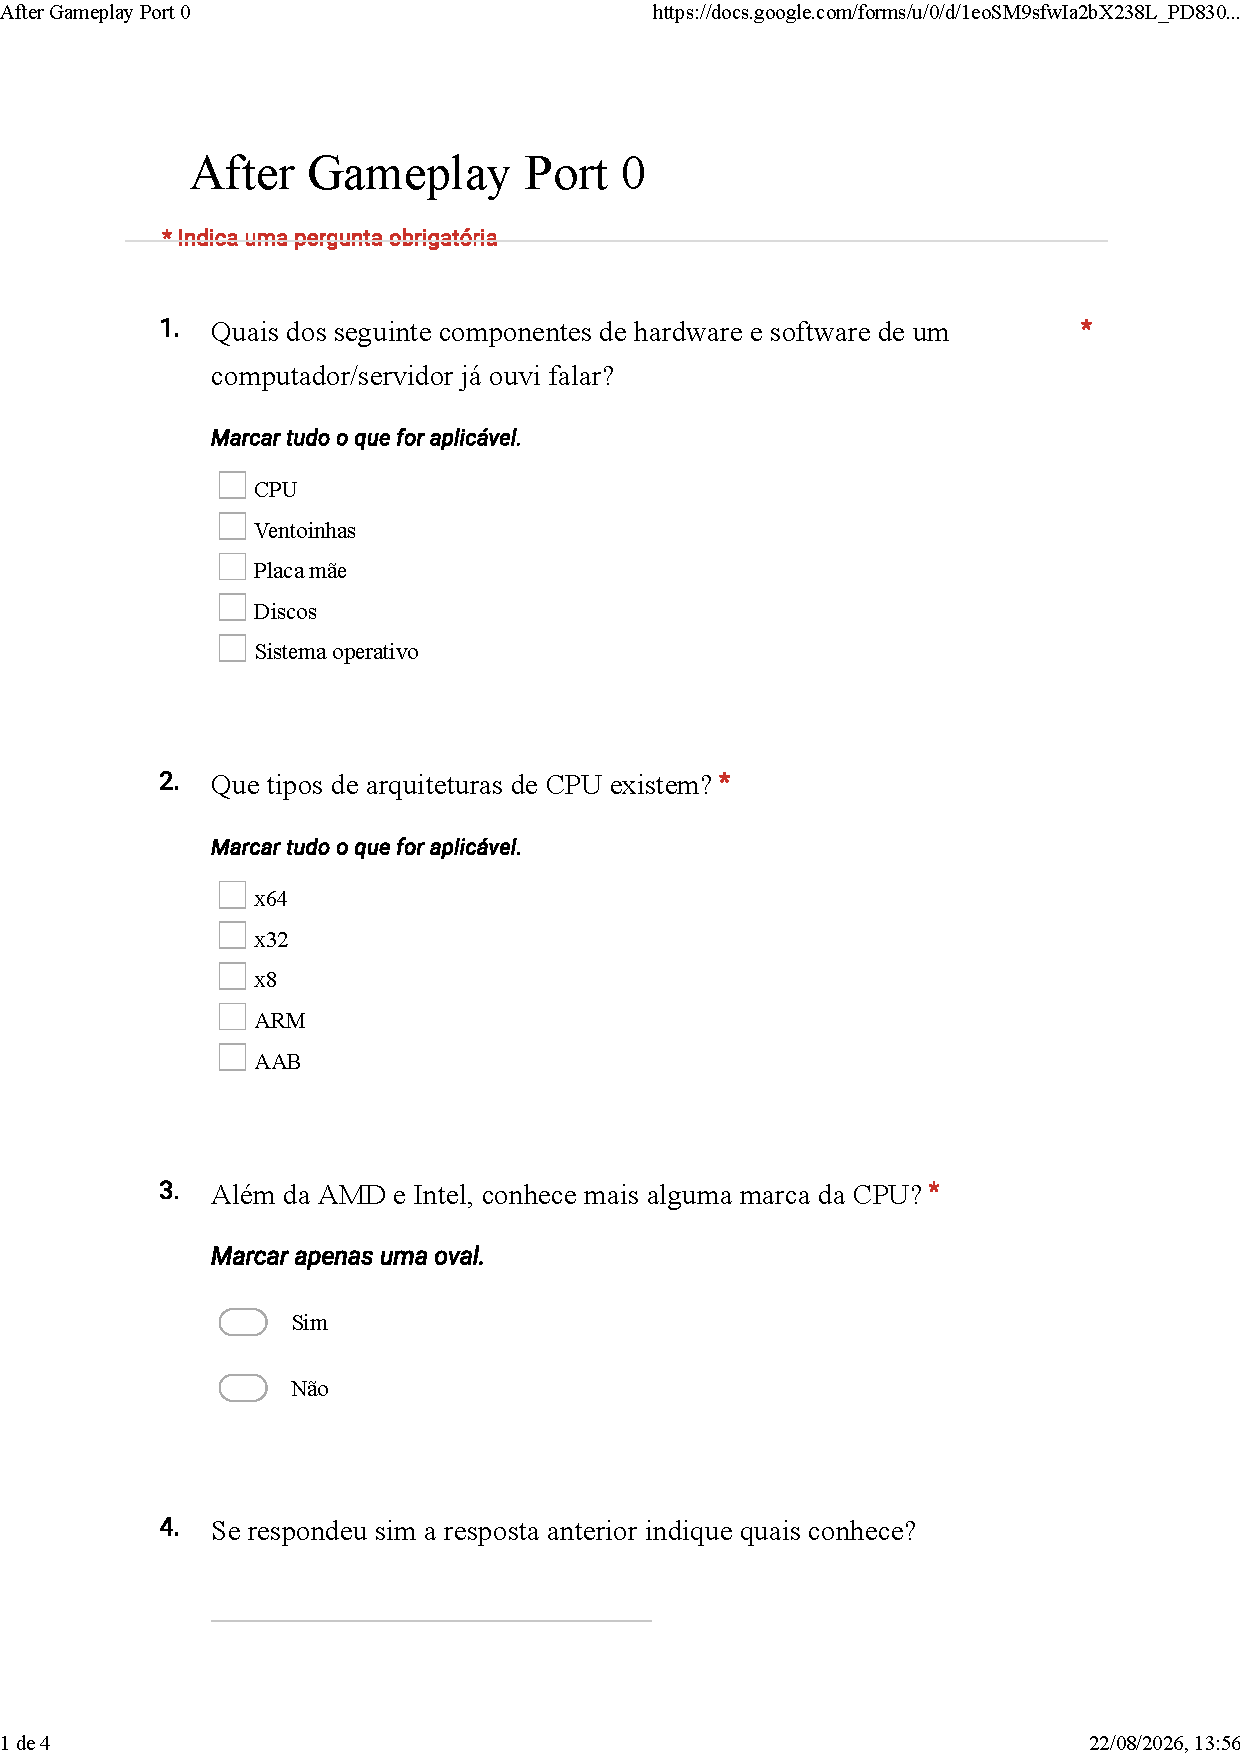
\includepdf[
  pages=-,
  pagecommand={\refstepcounter{section}\label{Anexo:depois_jogo}},
  scale=0.8
]{./forms/after.pdf}

\end{document}